\documentclass[a4paper,12pt]{article}

\usepackage{"D:/Document\space &\space Files/Documents/Dropbox/Study/tools/latex/mystyle"}

% Table of Contents. Spacing
% https://tex.stackexchange.com/questions/56546/how-to-change-spaces-between-items-in-table-of-contents
\usepackage{tocloft}
%\renewcommand\cftchapafterpnum{\vskip10pt}
\renewcommand\cftsecafterpnum{\vskip10pt}
\renewcommand\cftsubsecafterpnum{\vskip5pt}

\graphicspath{ {images/} }

\DeclareMathOperator{\cour}{\sigma}
\newcommand{\myvspaceOne}{-4.45cm}

% \DeclareMathOperator{\tg}{tg} = \newcommand{\tg}{\mathop{\mathrm{tg}}\nolimits}

% \includeonly{task02}

%\author{Алексеев Василий, 474}
%\title{Курсовая}
%\date{21 мая 2017}

\begin{document}
\begin{titlepage}

\newcommand{\HRule}{\rule{\linewidth}{0.5mm}} % Defines a new command for the horizontal lines, change thickness here

\center % Center everything on the page

\textsc{\LARGE МФТИ}\\[0.5cm]
\textsc{\Large ФУПМ, 474}\\[0.5cm] % Major heading such as course name
\textsc{\large Вычислительная математика}\\[1.5cm] % Minor heading such as course title

\vspace{3cm}

\HRule \\[0.4cm]
{ \huge \bfseries Курсовая работа}\\[0.3cm] % Title of your document
\HRule \\[1.5cm]

\Large %\emph{Автор:}\\
\textsc{Алексеев} Василий\\[3cm]

\vspace{\fill}

{\large 22 Мая 2017}\\[0.2cm] % Date, change the \today to a set date if you want to be precise

%\vfill
\end{titlepage}

  %\thispagestyle{empty}
  %\newpage
  
  \pagenumbering{arabic}
  
{
\hypersetup{linkcolor=black}
\tableofcontents
}		
  \newpage

\section{Введение}
  В данной работе предлагается несколько методов численного решения задачи, связанной с уравнением Хопфа.
  Проводится исследование предложенных схем на аппроксимацию и устойчивость.
  
\section{Задача}
  \begin{equation}
    \left\{
    \begin{aligned}
      &\frac{\partial u}{\partial t} + u \frac{\partial u}{\partial x} = 0, & &0 < x < 2,\ t > 0\\
      &u(0, x) = f(x) & &{}\\
      &u(t, 0) = f(0) & &{}
    \end{aligned}
    \right.
    \label{eq:task}
  \end{equation}
  
  \jp
  Предлагаемые далее способы решения задачи (\ref{eq:task}) иллюстрировались на примере двух функций
  \begin{equation}
    \begin{aligned}
      &f_1(x) = 1 - x\\
      &f_2(x) = x
    \end{aligned}
    \label{eq:funcs}
  \end{equation}
  
  \jp
  Шаг по пространству
  \begin{equation}
    \begin{aligned}
      &h_1 = 0.050\\
      &h_2 = 0.025
    \end{aligned}
    \label{eq:steps}
  \end{equation}
  
  \jp
  Шаг по времени $\tau$ выбирался при заданном $h$, так чтобы число Куранта
  \begin{equation}
    \sigma \equiv \tau \Big/ h
  \end{equation}
  было меньше единицы.
  Если говорить точнее, рассматривалось два значения числа Куранта
  \begin{equation}
    \sigma \in \{0.5,\ 0.9\}
    \label{eq:cours}
  \end{equation}
  \newpage
  
\section{Методы}

\subsection{"`Наивный"'}
\label{sec:silly}
  \begin{equation}
    \left\{
    \begin{aligned}
      &\frac{u_m^{n+1} - u_m^{n-1}}{2 \tau} + u_m^n \frac{u_{m+1}^n - u_{m-1}^n}{2h} = 0, & &m = 1 \div (M-1),\ 
        n = 1 \div (N-1)\\
      &u_m^0 = f_m & &{}\\
      &u_0^n = f_0 & &{}\\
      &u_m^1 = f_m - f_m f_m' \tau & &{}\\
      &\frac{u_M^{n+1} - u_m^n}{\tau} - \frac{w_M^n - w_{M-1}^n}{h} = 0 & &{}\\
      &w_m^n = (u_m^n)^2 \Big/ 2 & &{}
    \end{aligned}
    \right.
    \label{eq:silly}
  \end{equation}
  
  \jp
  Поясним выражение для первого слоя $u_m^1$
  
  \begin{equation*}
  \begin{split}
    u_m^1 &= u_m^0 + (u_m^0)'_t \tau\\
      &= u_m^0 - u_m^0(u_m^0)'_x \tau\\
      &= f_m - f_m f_m' \tau
  \end{split}
  \end{equation*}
  
  \jp
  \emph{Аппроксимация}
  \jp
  Из основного уравнения: $O(\tau^2) + \|u_m^n\| \cdot O(h^2) = O(\tau^2, h^2)$.\sp
  Из начального условия для первого слоя: $O(\tau^2)$.\sp
  Из условия на правой границе $u_M$: $O(\tau, h)$.\sp
  Итоговый порядок аппроксимации: $O(\tau, h)$.
  
  \jp
  \emph{Устойчивость}
  \jp
  Используем спектральный признак.
  Полагаем $u_m^n \hm= \ld^n e^{im\phi}$.
  Подставляем в основное уравнение (замораживая коэффициент при пространственной производной)\jp
  $\dfrac{\ld - 1/\ld}{2\tau} + a \dfrac{e^{i\phi} - e^{-i\phi}}{2h} = 0$\sp
  $\ld^2 + \dfrac{2a\tau}{h}i\sin{\phi} \ld - 1 = 0$\jp
  По теореме Виета, получаем, что\jp
  $\ld_1 \ld_2 = -1$\jp
  Выражение для корней\jp
  $\ld = -\dfrac{a\tau\sin{\phi}}{h} i \pm \sqrt{1 - \left(\dfrac{a\tau\sin{\phi}}{h}\right)^2}$\jp
  Видно, что при выполнении условия
  \[
    \left|\frac{a\tau\sin{\phi}}{h}\right| \leq \frac{\|u_m^n\| \tau}{h} \leq 1
  \]
  схема (\ref{eq:silly}) устойчива.
  \jp
  По результатам вычислительных экспериментов построены графики, представленные в таблице \ref{plot:silly}.
  \newpage
  
\subsection{Лакс}
\label{sec:lax}
  \begin{equation}
    \left\{
    \begin{aligned}
      &\frac{u_m^{n+1} - \frac{1}{2} \Bigl(u_{m+1}^n + u_{m-1}^n\Bigr)}{\tau} + \frac{w_{m+1}^n - w_{m-1}^n}{2h} = 0, & &m = 1 \div (M-1),\ n = 0 \div (N-1)\\
      &u_m^0 = f_m & &{}\\
      &u_0^m = f_0 & &{}\\
      &\frac{u_M^{n+1} - u_m^n}{\tau} - \frac{w_M^n - w_{M-1}^n}{h} = 0 & &{}\\
      &w_m^n = (u_m^n)^2 \Big/ 2 & &{}
    \end{aligned}
    \right.
    \label{eq:lax}
  \end{equation}
  
  \jp
  \emph{Аппроксимация}
  \jp
  Подставляя в основное разностное уравнение проекцию точного решения $[u]$ и раскладывая всё в окрестности точки $[u_m^n]$, получаем порядок $O\left(\tau, h^2, \dfrac{h^2}{\tau}\right)$.
  С учётом уравнения для границы $u_M$, получаем в итоге аппроксимацию порядка $O\left(\tau, h, \dfrac{h^2}{\tau}\right)$.
  
  \jp
  \emph{Устойчивость}
  \jp
  $u_m^n \hm= w_n^m \hm= \ld^n e^{im\phi}$\jp
  Подставляя в уравнение, получаем\jp
  $\dfrac{\ld - \frac{1}{2} (e^{i\phi} + e^{-i\phi})}{\tau} + \dfrac{e^{i\phi} - e^{-i\phi}}{2h} = 0$\jp
  $\ld = \underbrace{\cos{\phi}}_{x} + i \underbrace{\left(-\dfrac{\tau}{h} \sin{\phi}\right)}_{y}$\jp
  $x^2 + \dfrac{y^2}{(\tau / h)^2} = 1$\jp
  Получаем условие для устойчивости по спектральному признаку
  \[
    \frac{\tau}{h} \leq 1
  \]
  
  \noi
  Графики для расчётов по схеме Лакса находятся в таблице \ref{plot:lax}.
  \newpage

\subsection{Курант-Изаксон-Рис}
\label{sec:cir}
  \begin{equation}
    \left\{
    \begin{aligned}
      &\frac{u_m^{n+1} - u_m^n}{\tau} +
        \left\{
        \begin{aligned}
          &\frac{w_{m+1}^n - w_m^n}{h} = 0,\ u_m^n < 0\\
          &\frac{w_{m}^n - w_{m-1}^n}{h} = 0,\ u_m^n > 0
        \end{aligned}
        \right\} = 0,
        & &m = 1 \div (M-1),\ n = 0 \div (N-1)\\
      &u_m^0 = f_m & &{}\\
      &u_0^m = f_0 & &{}\\
      &\frac{u_M^{n+1} - u_m^n}{\tau} - \frac{w_M^n - w_{M-1}^n}{h} = 0 & &{}\\
      &w_m^n = (u_m^n)^2 \Big/ 2 & &{}
    \end{aligned}
    \right.
    \label{eq:cir}
  \end{equation}
  
  \jp
  \emph{Аппроксимация}
  \jp
  Данная схема похожа на схему (\ref{eq:silly}), только теперь учитывается знак тангенса угла наклона характеристики $dx / dt$.
  Поэтому порядок аппроксимации также $O(\tau, h)$.
  
  \jp
  \emph{Устойчивость}
  \jp
  $u_m^n \hm= \ld^n e^{im\phi}$\jp
  Подставляя выражение для $u_m^n$, например, в уравнение при $u_m^n < 0$, получаем\jp
  $\dfrac{\ld - 1}{\tau} + \dfrac{e^{i\phi} - 1}{h} = 0$\jp
  $\ld = 1 - \dfrac{\tau}{h} \left(\vphantom{\dfrac{1}{1}}e^{i\phi} - 1\right)$\jp
  Схему можно считать устойчивой при $\tau \Big/ h \to 0$.
  \jp
  Иллюстрации работы метода на примере функций (\ref{eq:funcs}) находятся в таблице \ref{plot:cir}.
  \newpage

\subsection{Лакс-Вендрофф}
\label{sec:lax-vendroff}
  \begin{equation}
    \left\{
    \begin{aligned}
      &
        \left\{
        \begin{aligned}
          &\frac{u_{m+1/2}^{n+1/2} - \frac{1}{2} \Bigl(u_{m+1}^n + u_m^n\Bigr)}{\tau / 2} +
            \frac{w_{m+1}^n - w_m^n}{h} = 0\\
          &\frac{u_{m-1/2}^{n+1/2} - \frac{1}{2} \Bigl(u_{m}^n + u_{m-1}^n\Bigr)}{\tau / 2} +
            \frac{w_{m}^n - w_{m-1}^n}{h} = 0\\
        \end{aligned}
        \right. & &{}\\
      &\frac{u_m^{n+1} - u_m^n}{\tau} + \frac{w_{m+1/2}^{n+1/2} - w_{m-1/2}^{n+1/2}}{h} = 0, &
        &m = 1 \div (M-1),\ n = 0 \div (N-1)\\
      &u_m^0 = f_m & &{}\\
      &u_0^m = f_0 & &{}\\
      &\frac{u_M^{n+1} - u_m^n}{\tau} - \frac{w_M^n - w_{M-1}^n}{h} = 0 & &{}\\
      &w_m^n = (u_m^n)^2 \Big/ 2 & &{}
    \end{aligned}
    \right.
    \label{eq:lax-vendroff}
  \end{equation}
  
  \jp
  \emph{Аппроксимация}
  \jp
  Подставляя в первое уравнение-предиктор проекцию решения и раскладывая всё около $[u_m^n]$, а также учитывая, что
  \[
    \begin{aligned}
      &u_t + w_x = 0\\
      &u_{tt} + w_{xt} = 0\\
      &u_{tx} + w_{xx} = 0
    \end{aligned}
  \]
  получаем первый порядок по времени и пространству $O(\tau, h)$.
  Очевидно, второе уравнение-предиктор даст то же самое.
  Теперь обратимся к уравнению-корректору.
  Проделывая и с ним аналогичные преобразования, получаем порядок $O(\tau, h^2)$.
  В итоге порядок аппроксимации $O(\tau, h)$.
  
  \jp
  \emph{Устойчивость}
  \jp
  $u_m^n \hm= w_m^n \hm= \ld^n e^{im\phi}$\jp
  Подставляем в корректор\jp
  $\dfrac{\ld - 1}{\tau} + \dfrac{\sqrt{\ld}(e^{i\phi/2} - e^{-i\phi/2})}{h} = 0$\jp
  $\ld + 2i\sin{\dfrac{\phi}{2}} \cdot \dfrac{\tau}{h} \cdot \sqrt{\ld} - 1 = 0$\jp
  Не углубляясь в анализ расположения корней полученного уравнения, можно сразу сказать, что при $\tau \Big/ h \hm\to 0$ получаем $\ld \hm= 1$, и схему можно считать устойчивой.
  \jp
  С графиками можно ознакомиться в таблице \ref{plot:lax-vendroff}.

\subsection{МакКормак}
\label{sec:maccormack}
  \begin{equation}
    \left\{
    \begin{aligned}
      &
        \left\{
        \begin{aligned}
          &\frac{\td u_{m} - u_m^n}{\tau} + \frac{w_{m}^n - w_{m-1}^n}{h} = 0\\
          &\frac{\td u_{m+1} - u_{m+1}^n}{\tau} + \frac{w_{m+1}^n - w_{m}^n}{h} = 0\\
        \end{aligned}
        \right. & &{}\\
      &\frac{u_m^{n+1} - \frac{1}{2} \Bigl(u_{m}^n + \td u_m\Bigr)}{\tau} +
        \frac{\td w_{m+1} - \td w_{m}}{h} = 0, &
        &m = 1 \div (M-1),\ n = 0 \div (N-1)\\
      &u_m^0 = f_m & &{}\\
      &u_0^m = f_0 & &{}\\
      &\frac{u_M^{n+1} - u_m^n}{\tau} - \frac{w_M^n - w_{M-1}^n}{h} = 0 & &{}\\
      &w_m^n = (u_m^n)^2 \Big/ 2 & &{}
    \end{aligned}
    \right.
    \label{eq:maccormack}
  \end{equation}
  
  \jp
  \emph{Аппроксимация}
  \jp
  Выражая предсказания $\td u_m$ и $\td u_{m+1}$ из первых двух уравнений и подставляя это затем в третье уравнение, после разложения около $u_m^n$ получаем порядок аппроксимации $O(\tau, h)$.
  
  \jp
  \emph{Устойчивость}
  \jp
  $u_m^n \hm= w_m^n \hm= \ld^n e^{im\phi}$\jp
  Подставляем в корректор, принимая, что $\td u_m \equiv u_m^{n+1/2}$\jp
  $\dfrac{\ld - \frac{1}{2}\left(\vphantom{\frac{1}{2}}1 + \sqrt{\ld}\right)}{3\tau/4} +
    \dfrac{\sqrt{\ld}e^{i\phi} - \sqrt{\ld}}{h} = 0$\jp
  $\ld + \left(-\dfrac{1}{2} + \dfrac{3\tau/4}{h}e^{i\phi} - \dfrac{3\tau/4}{h}\right)\sqrt{\ld} - \dfrac{1}{2} = 0$\jp
  Устремим $\tau \Big/ h \to 0$.
  Тогда получаем\jp
  $\ld - \dfrac{1}{2} \sqrt{\ld} - \dfrac{1}{2} = 0$\jp
  $\left(\vphantom{\dfrac{1}{2}}\sqrt{\ld} - 1\right)\left(\sqrt{\ld} + \dfrac{1}{2}\right) = 0$\jp
  Получаем, что при $\tau \Big/ h \to 0$ максимальный $\ld$ по модулю равен $1$, поэтому схему можно считать устойчивой.
  \jp
  Построенные графики размещены в таблице \ref{plot:maccormack}.
  \newpage

\section{Заключение}
  В работе исследовалось несколько методов численного решения начально-краевой задачи с уравнением Хопфа с заданными значениями на левой границе (\ref{eq:task}): "`Наивный"' (схема крест) (\ref{eq:silly}), Лакс (\ref{eq:lax}), Курант-Изаксон-Рис (\ref{eq:cir}), Лакс-Вендрофф (\ref{eq:lax-vendroff}) и МакКормак (\ref{eq:maccormack}).
  
  Порядок аппроксимация на всех схемах составил $O(\tau, h)$.
  На некоторых схемах он мог бы быть и выше, но предложенное разностное уравнение для вычисления значений на правой границе (левый уголок), которое использовалось во всех схемах, обеспечивало лишь первый порядок аппроксимации по времени и пространству.
  
  Исследование устойчивости показало, что все представленные методы условно\-/устойчивы.
  Но при расчётах сеток для функций (\ref{eq:funcs}) и шага $h$ (\ref{eq:steps}) устойчивыми оказались лишь Лакс и Курант-Изаксон-Рис (по результатам для числа Куранта $\sigma \hm= 0.5$; для $\sigma \hm= 0.9$~---~не лучше, чем для $\sigma \hm= 0.5$).
  "`Наивный"' был устойчив только для функции $f_2$ из (\ref{eq:funcs}).
  Поведение Лакса-Вендроффа было неустойчивым около $x \hm= 1$ в случае $f_1$ из (\ref{eq:funcs}) и при $x \hm= 2$ при расчётах для $f_2$.
  При МакКормаке неустойчивости тоже были для обеих функций из (\ref{eq:funcs}), причём для $f_1$ пилообразные возмущения наблюдались на всём интервале $(0, 1)$, а для функции $f_2$~---~только на конце, при $x \hm{\lesssim} 2$.
  \newpage
  
  \iffalse
  \begin{figure}[p]
    \begin{subfigure}[t]{0.5\textwidth}
      \caption*{$\cour = 0.5,\ f_1,\ h = 0.050$}
      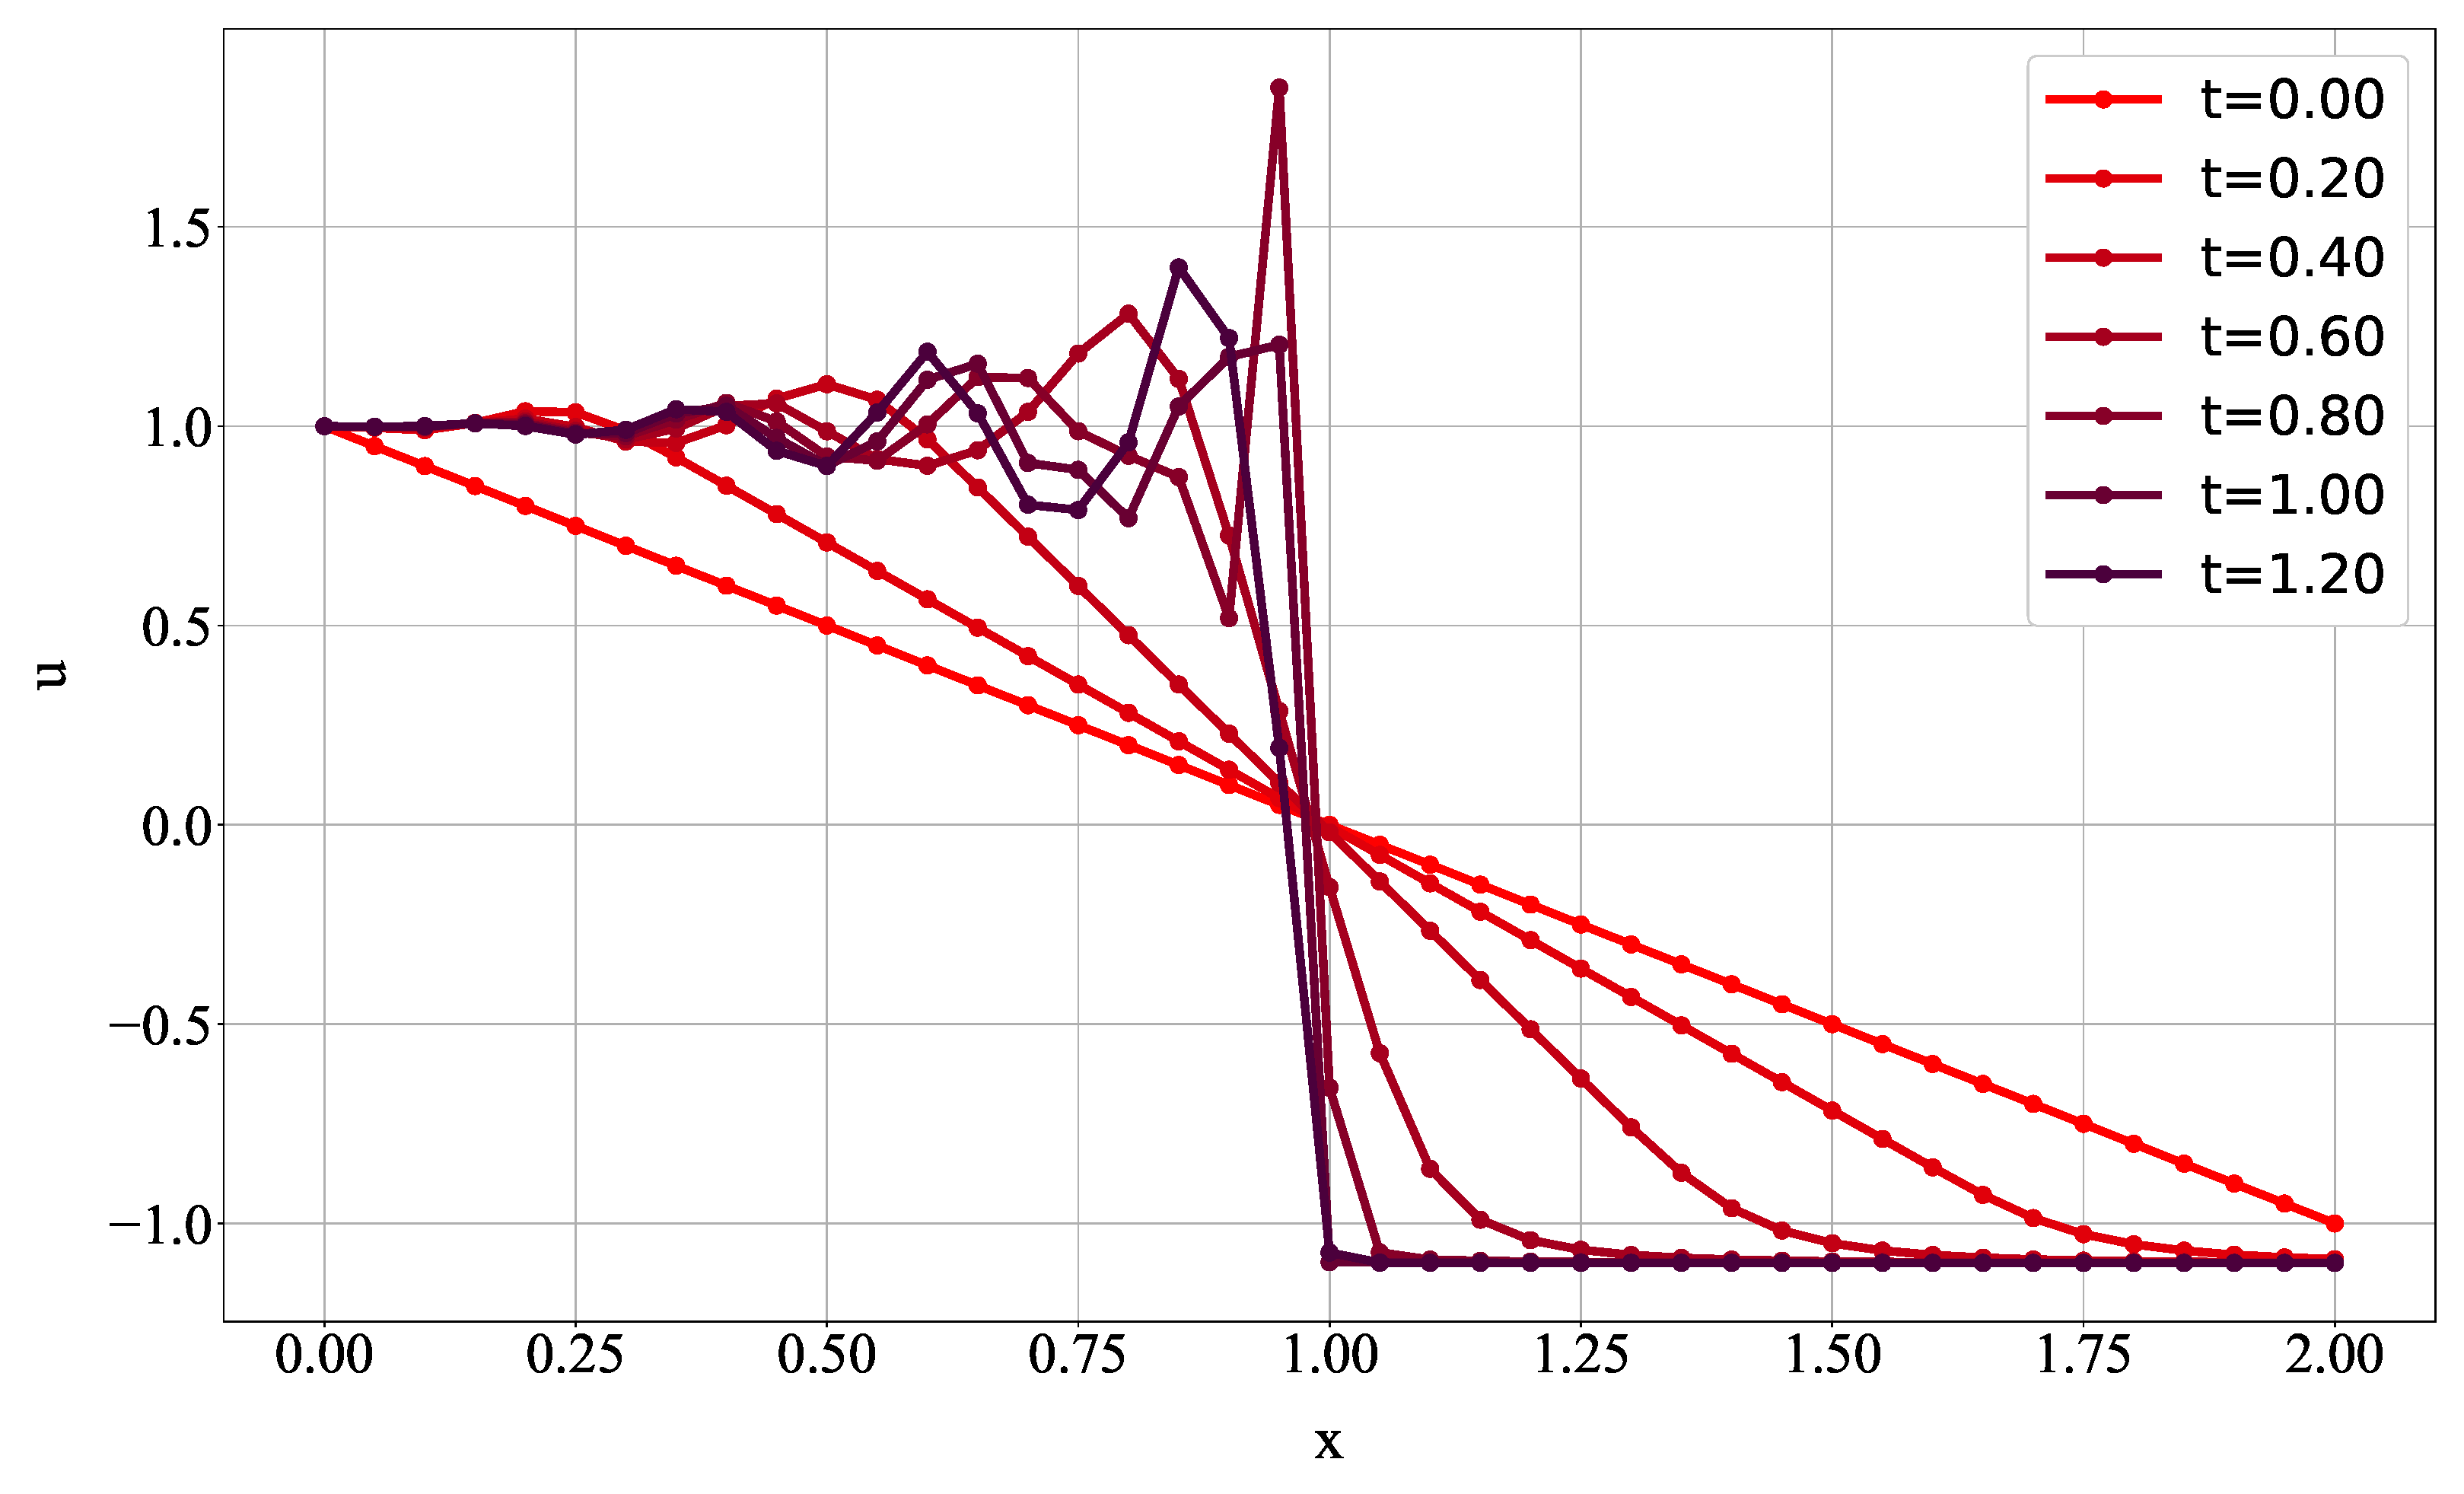
\includegraphics[width=\linewidth]{5.maccormack.cour05.f1050}
    \end{subfigure}
    ~
    \begin{subfigure}[t]{0.5\textwidth}
      \caption*{$\cour = 0.5,\ f_1,\ h = 0.025$}
      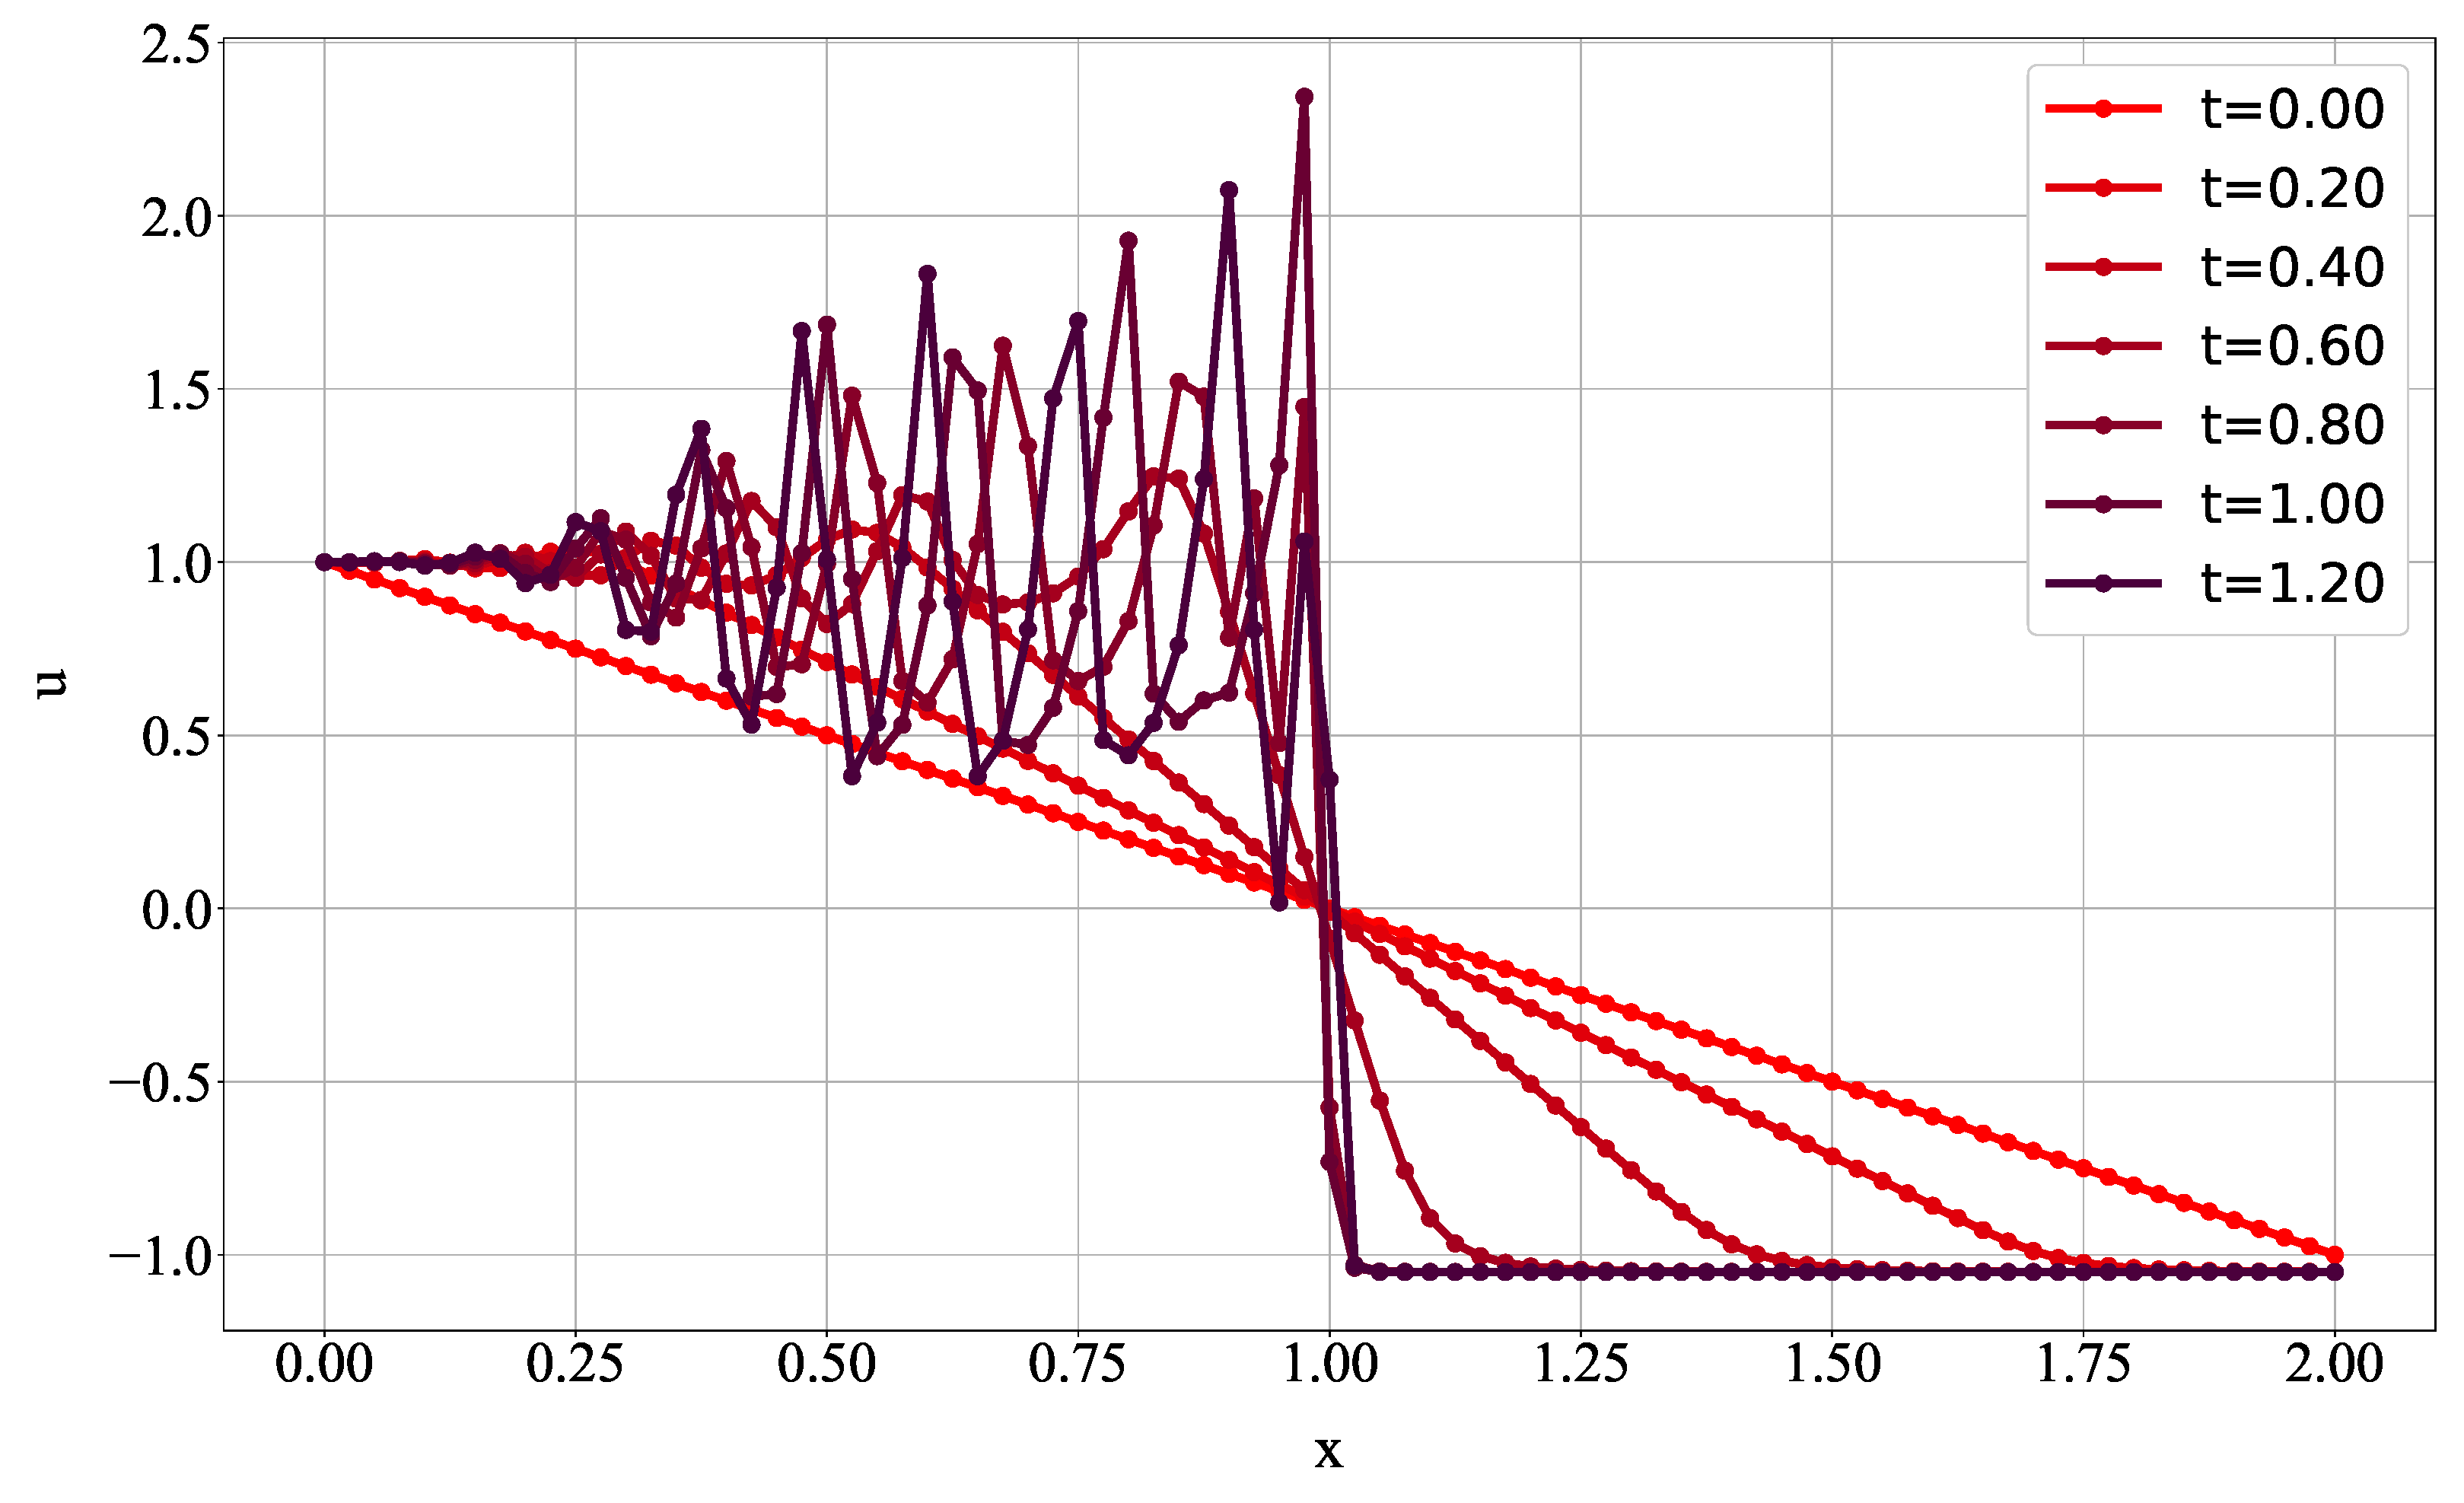
\includegraphics[width=\linewidth]{5.maccormack.cour05.f1025}
    \end{subfigure}
    
    \begin{subfigure}[t]{0.5\textwidth}
      \caption*{$\cour = 0.9,\ f_1,\ h = 0.050$}
      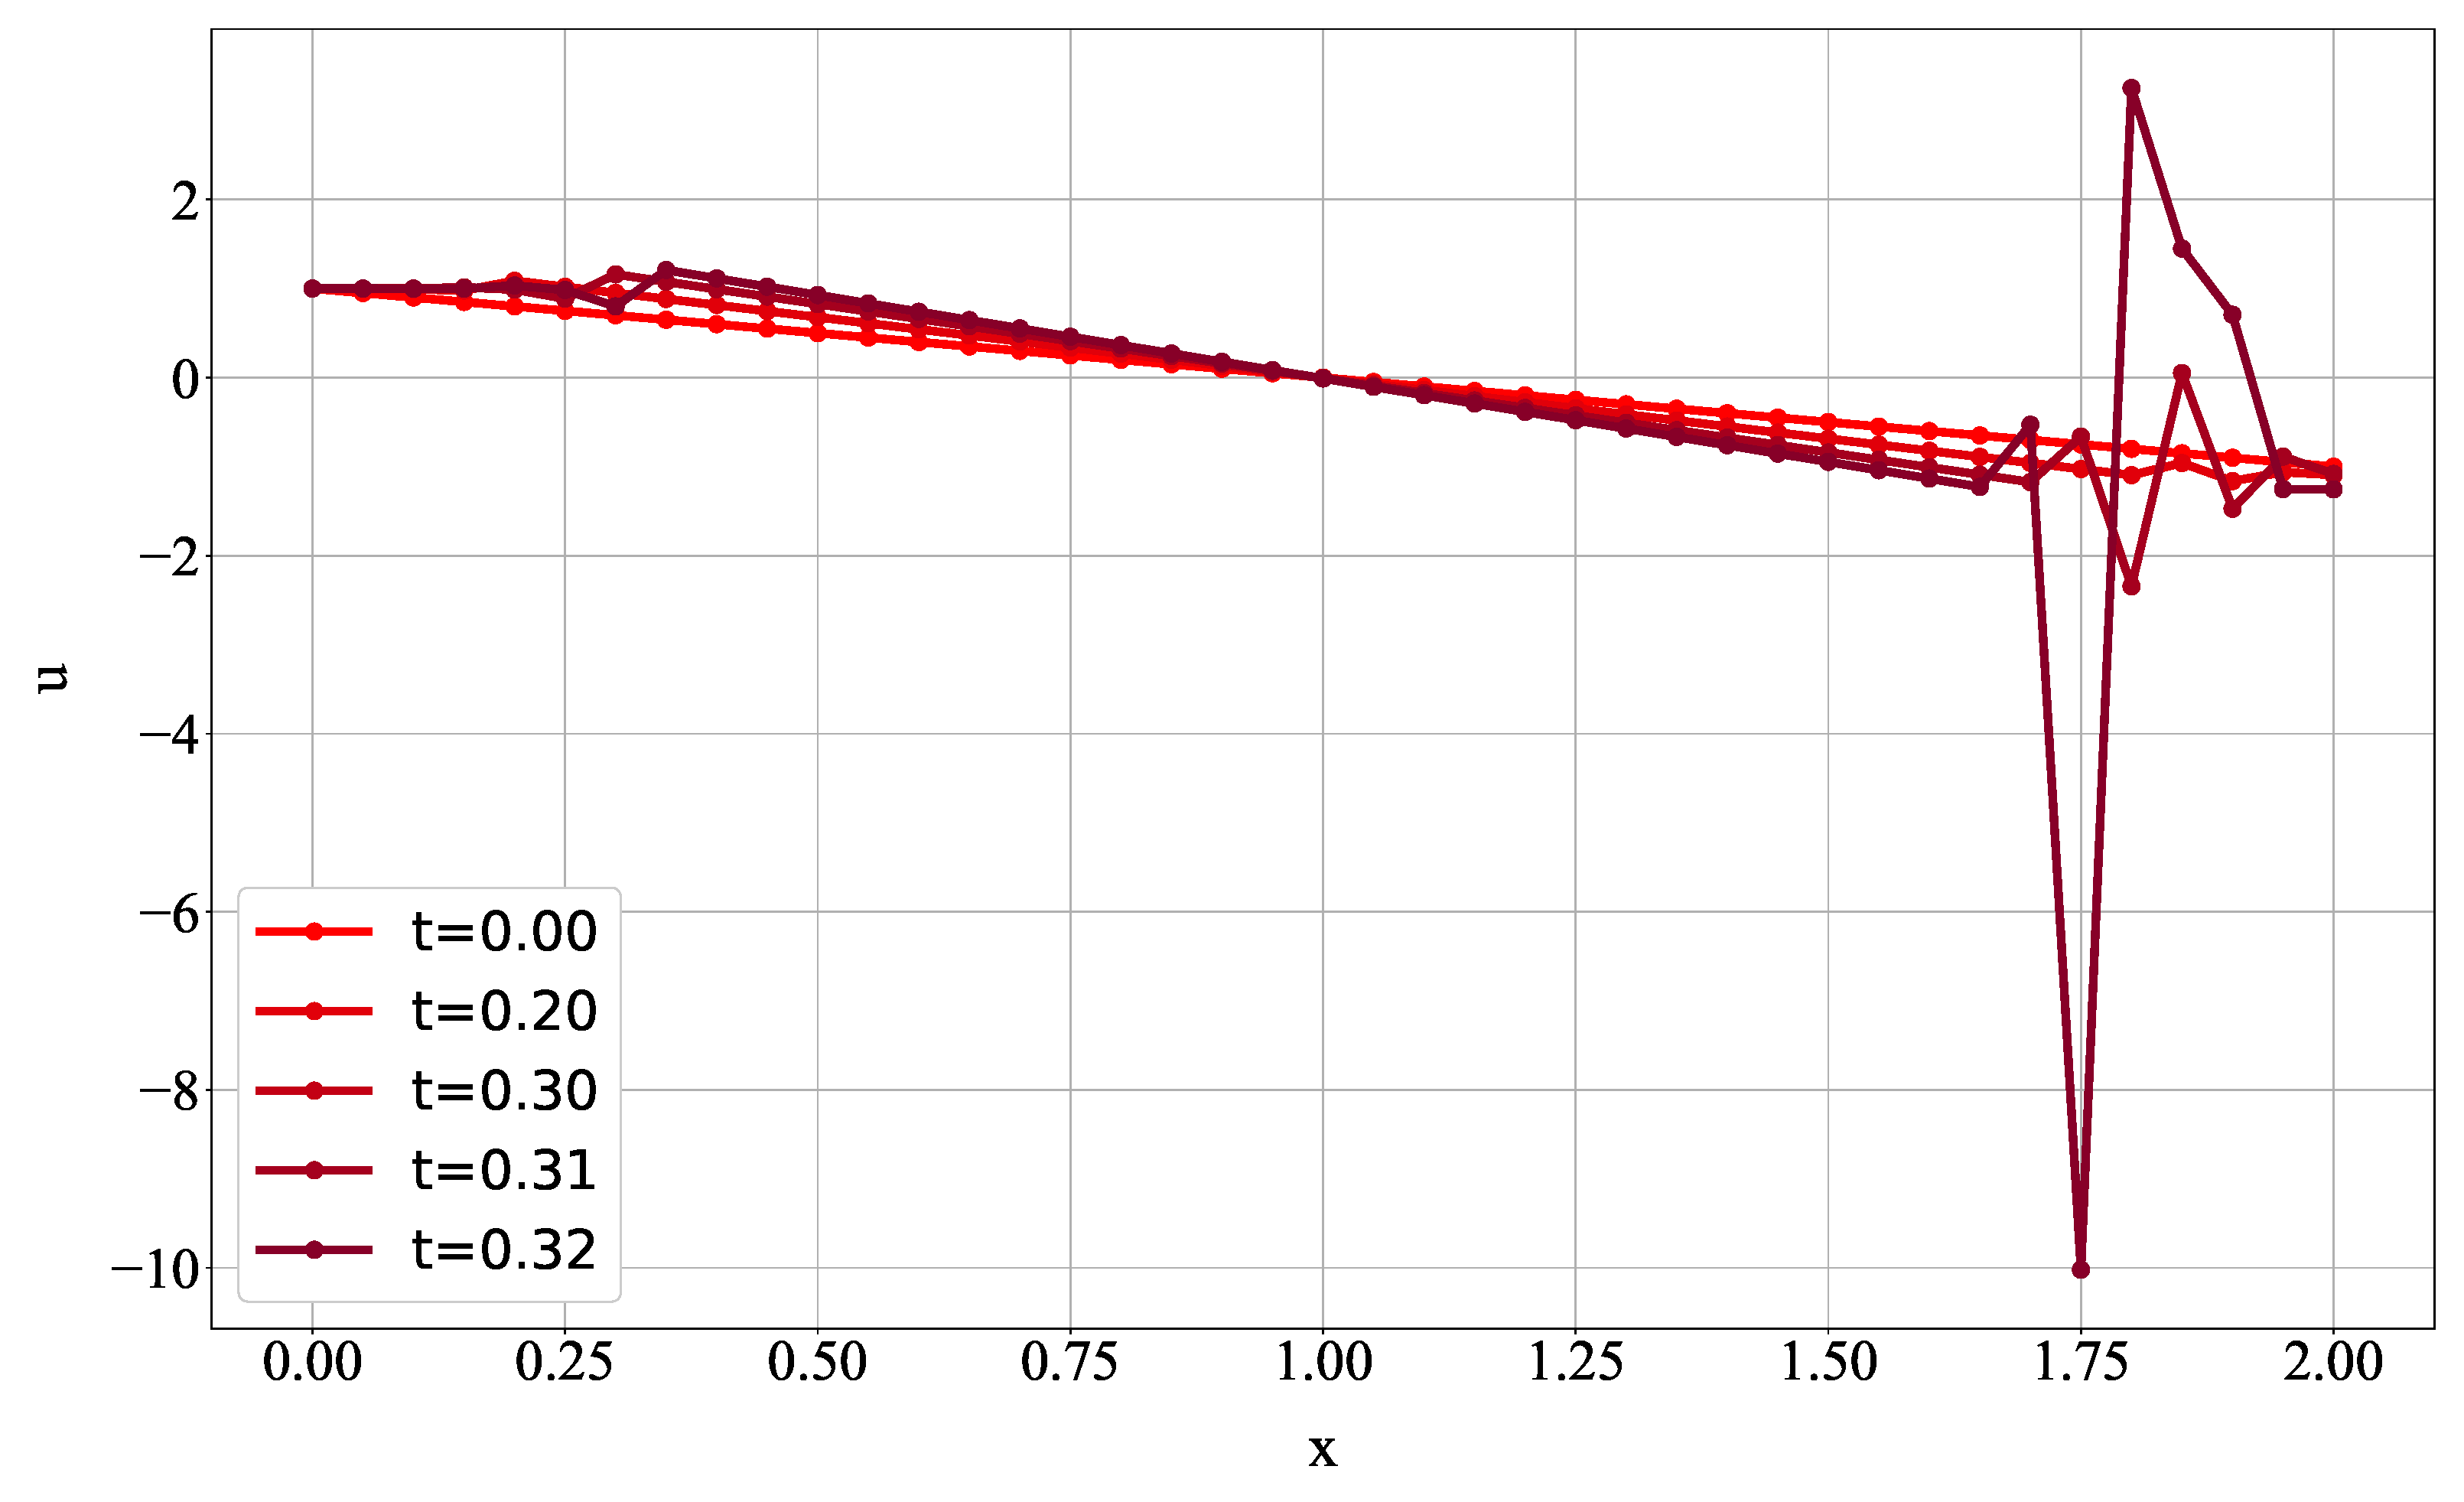
\includegraphics[width=\linewidth]{5.maccormack.cour09.f1050}
    \end{subfigure}
    ~
    \begin{subfigure}[t]{0.5\textwidth}
      \caption*{$\cour = 0.9,\ f_1,\ h = 0.025$}
      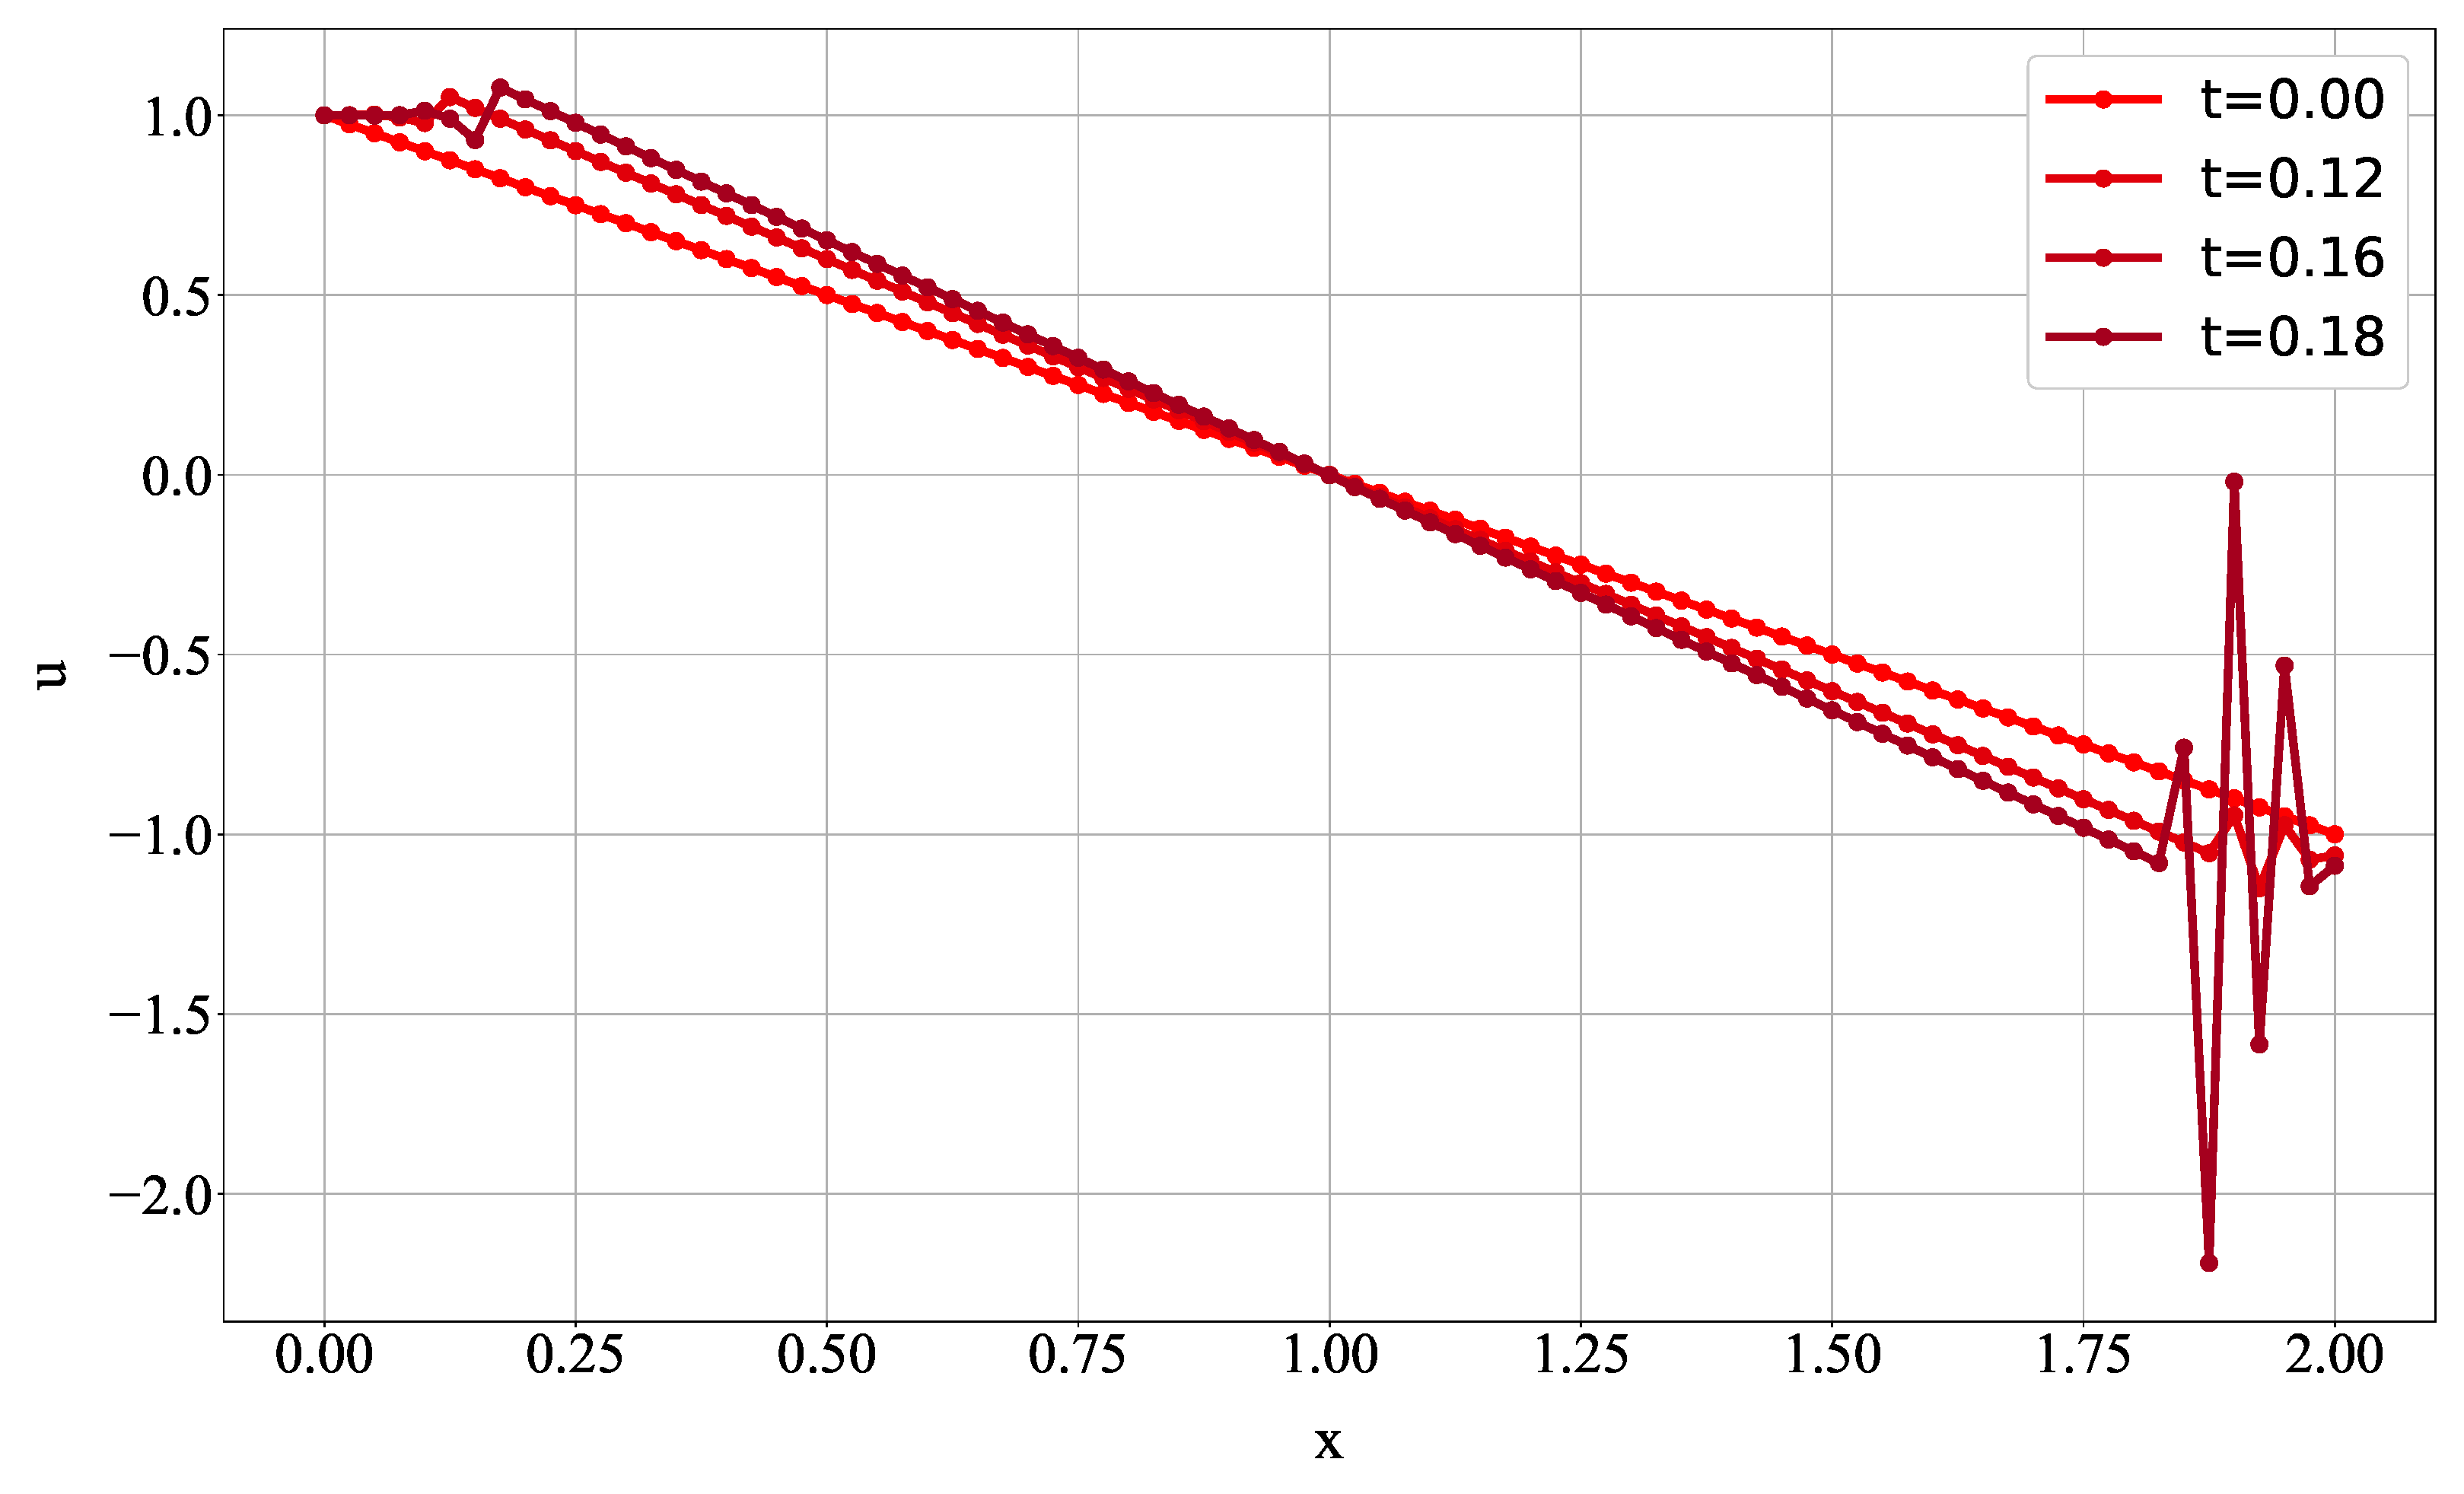
\includegraphics[width=\linewidth]{5.maccormack.cour09.f1025}
    \end{subfigure}
    %%
    \begin{subfigure}[t]{0.5\textwidth}
      \caption*{$\cour = 0.5,\ f_2,\ h = 0.050$}
      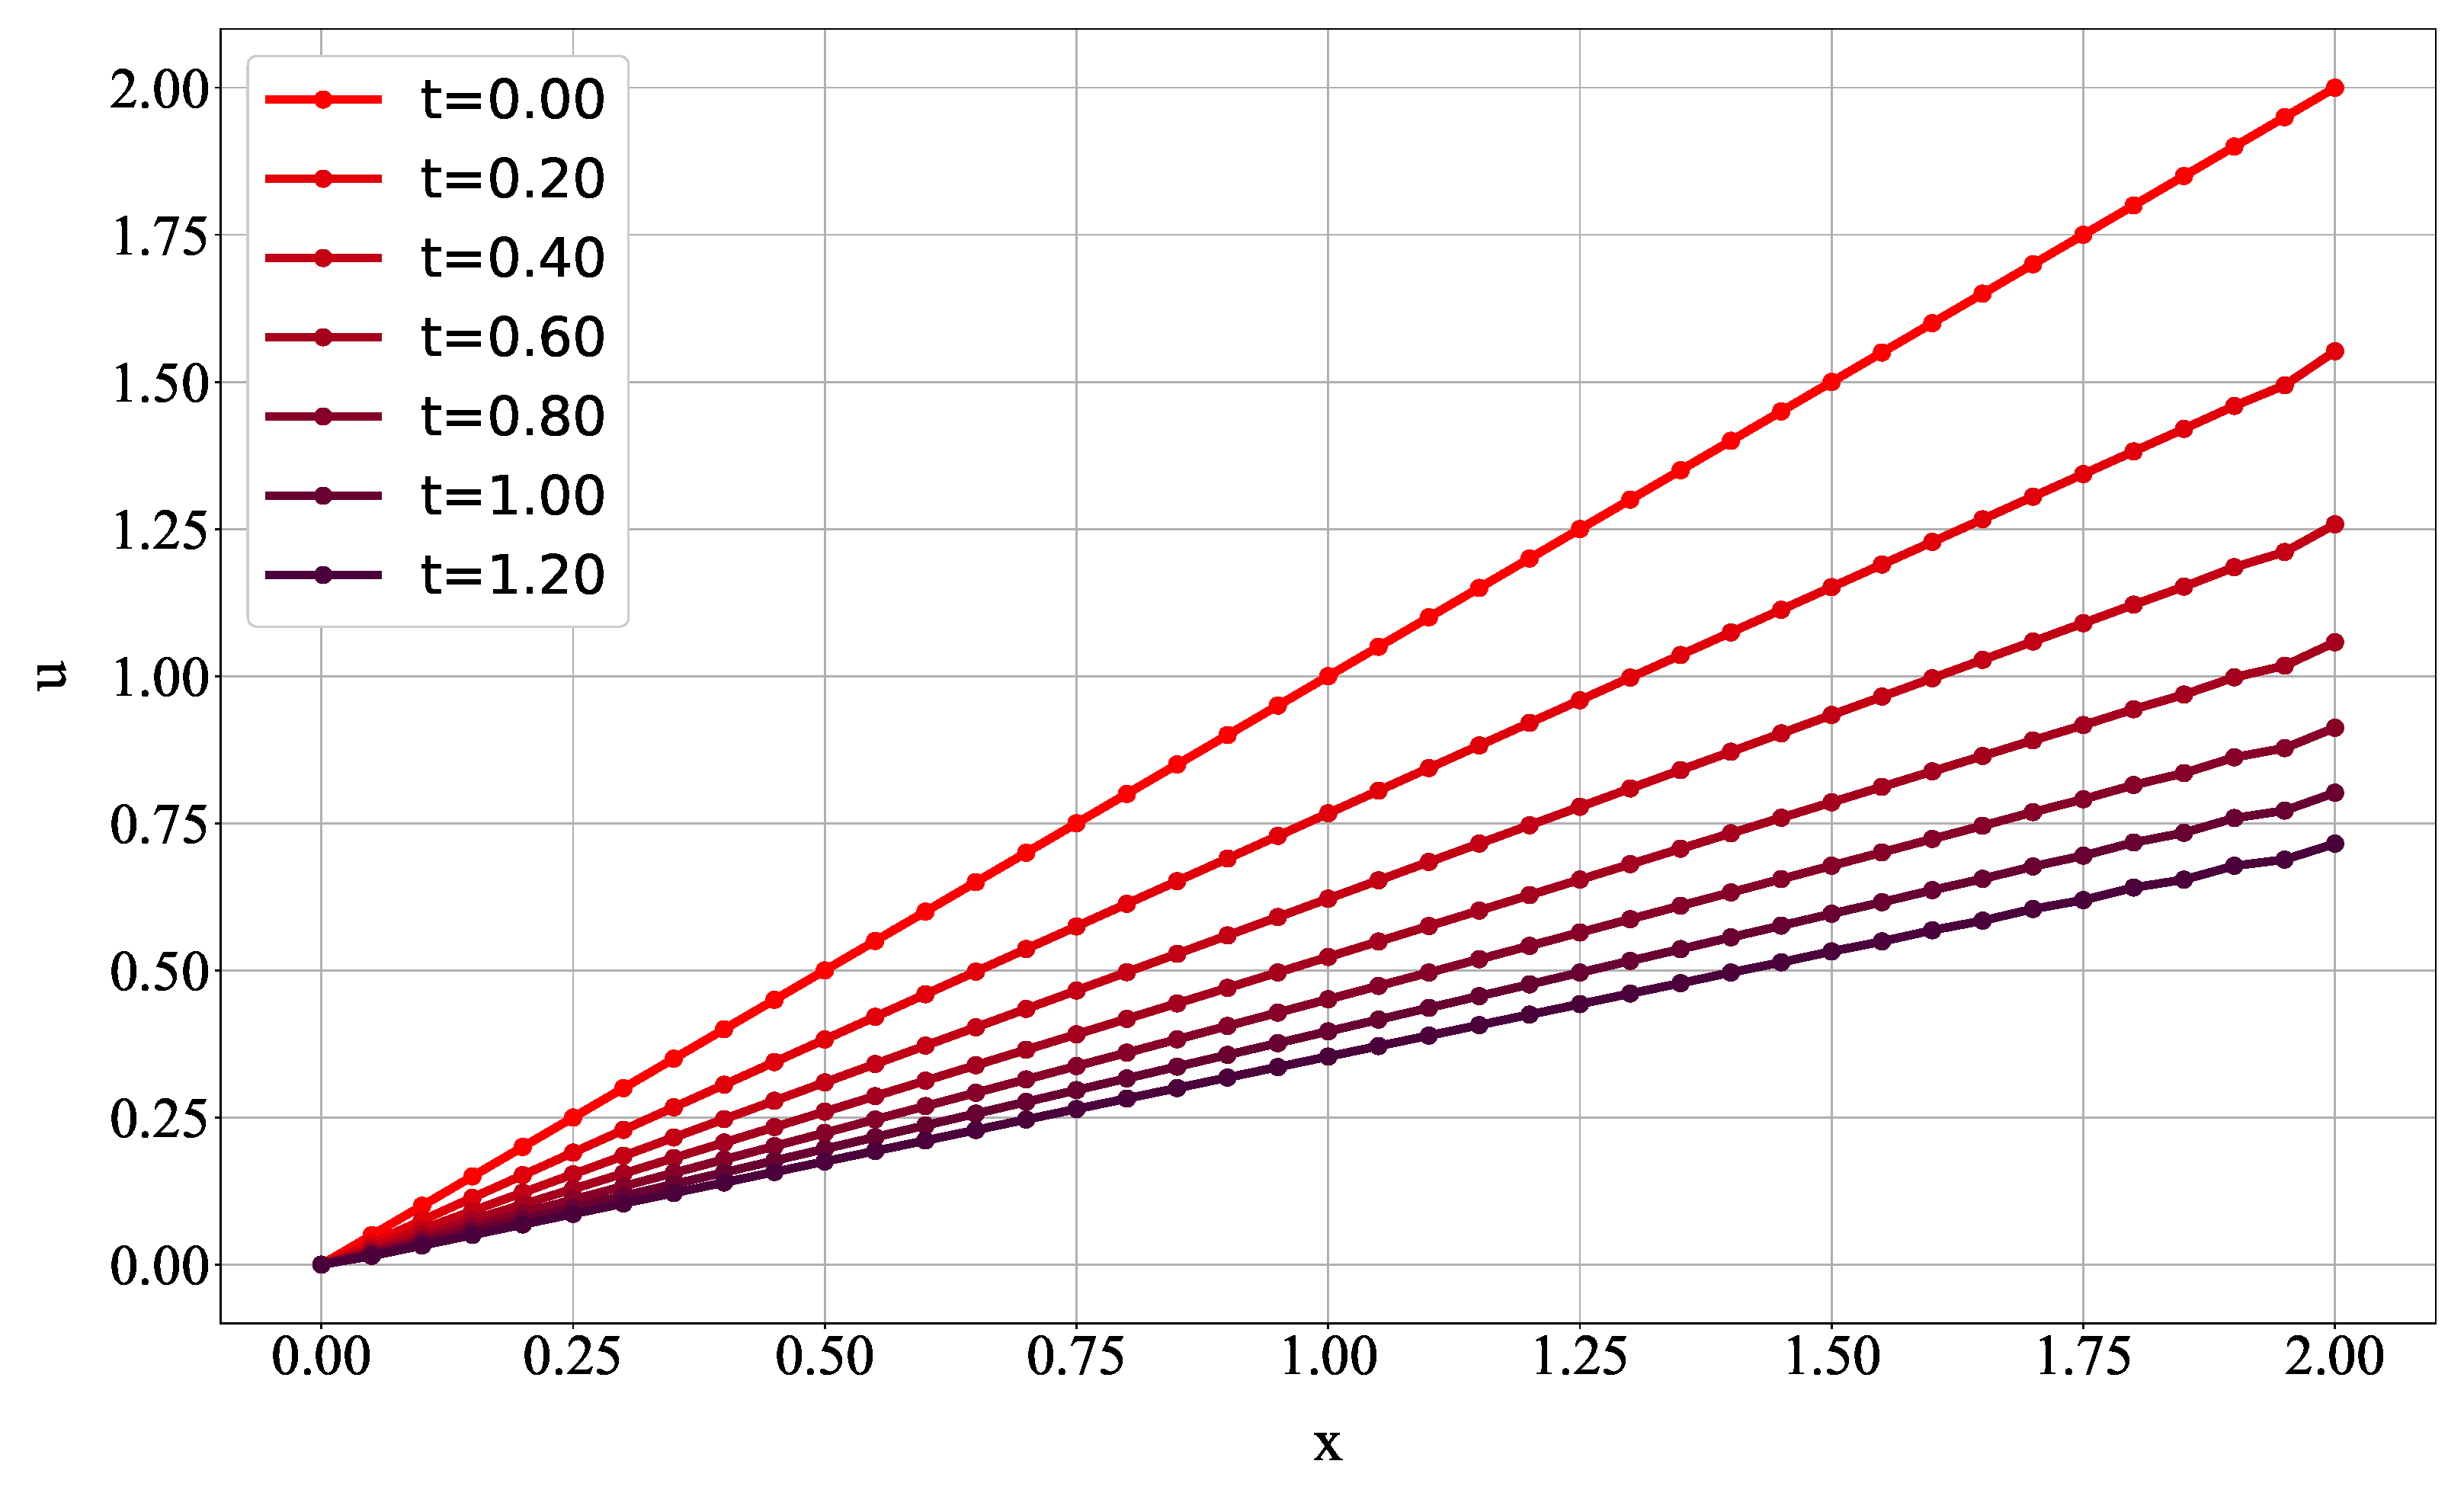
\includegraphics[width=\linewidth]{5.maccormack.cour05.f2050}
    \end{subfigure}
    ~
    \begin{subfigure}[t]{0.5\textwidth}
      \caption*{$\cour = 0.5,\ f_2,\ h = 0.025$}
      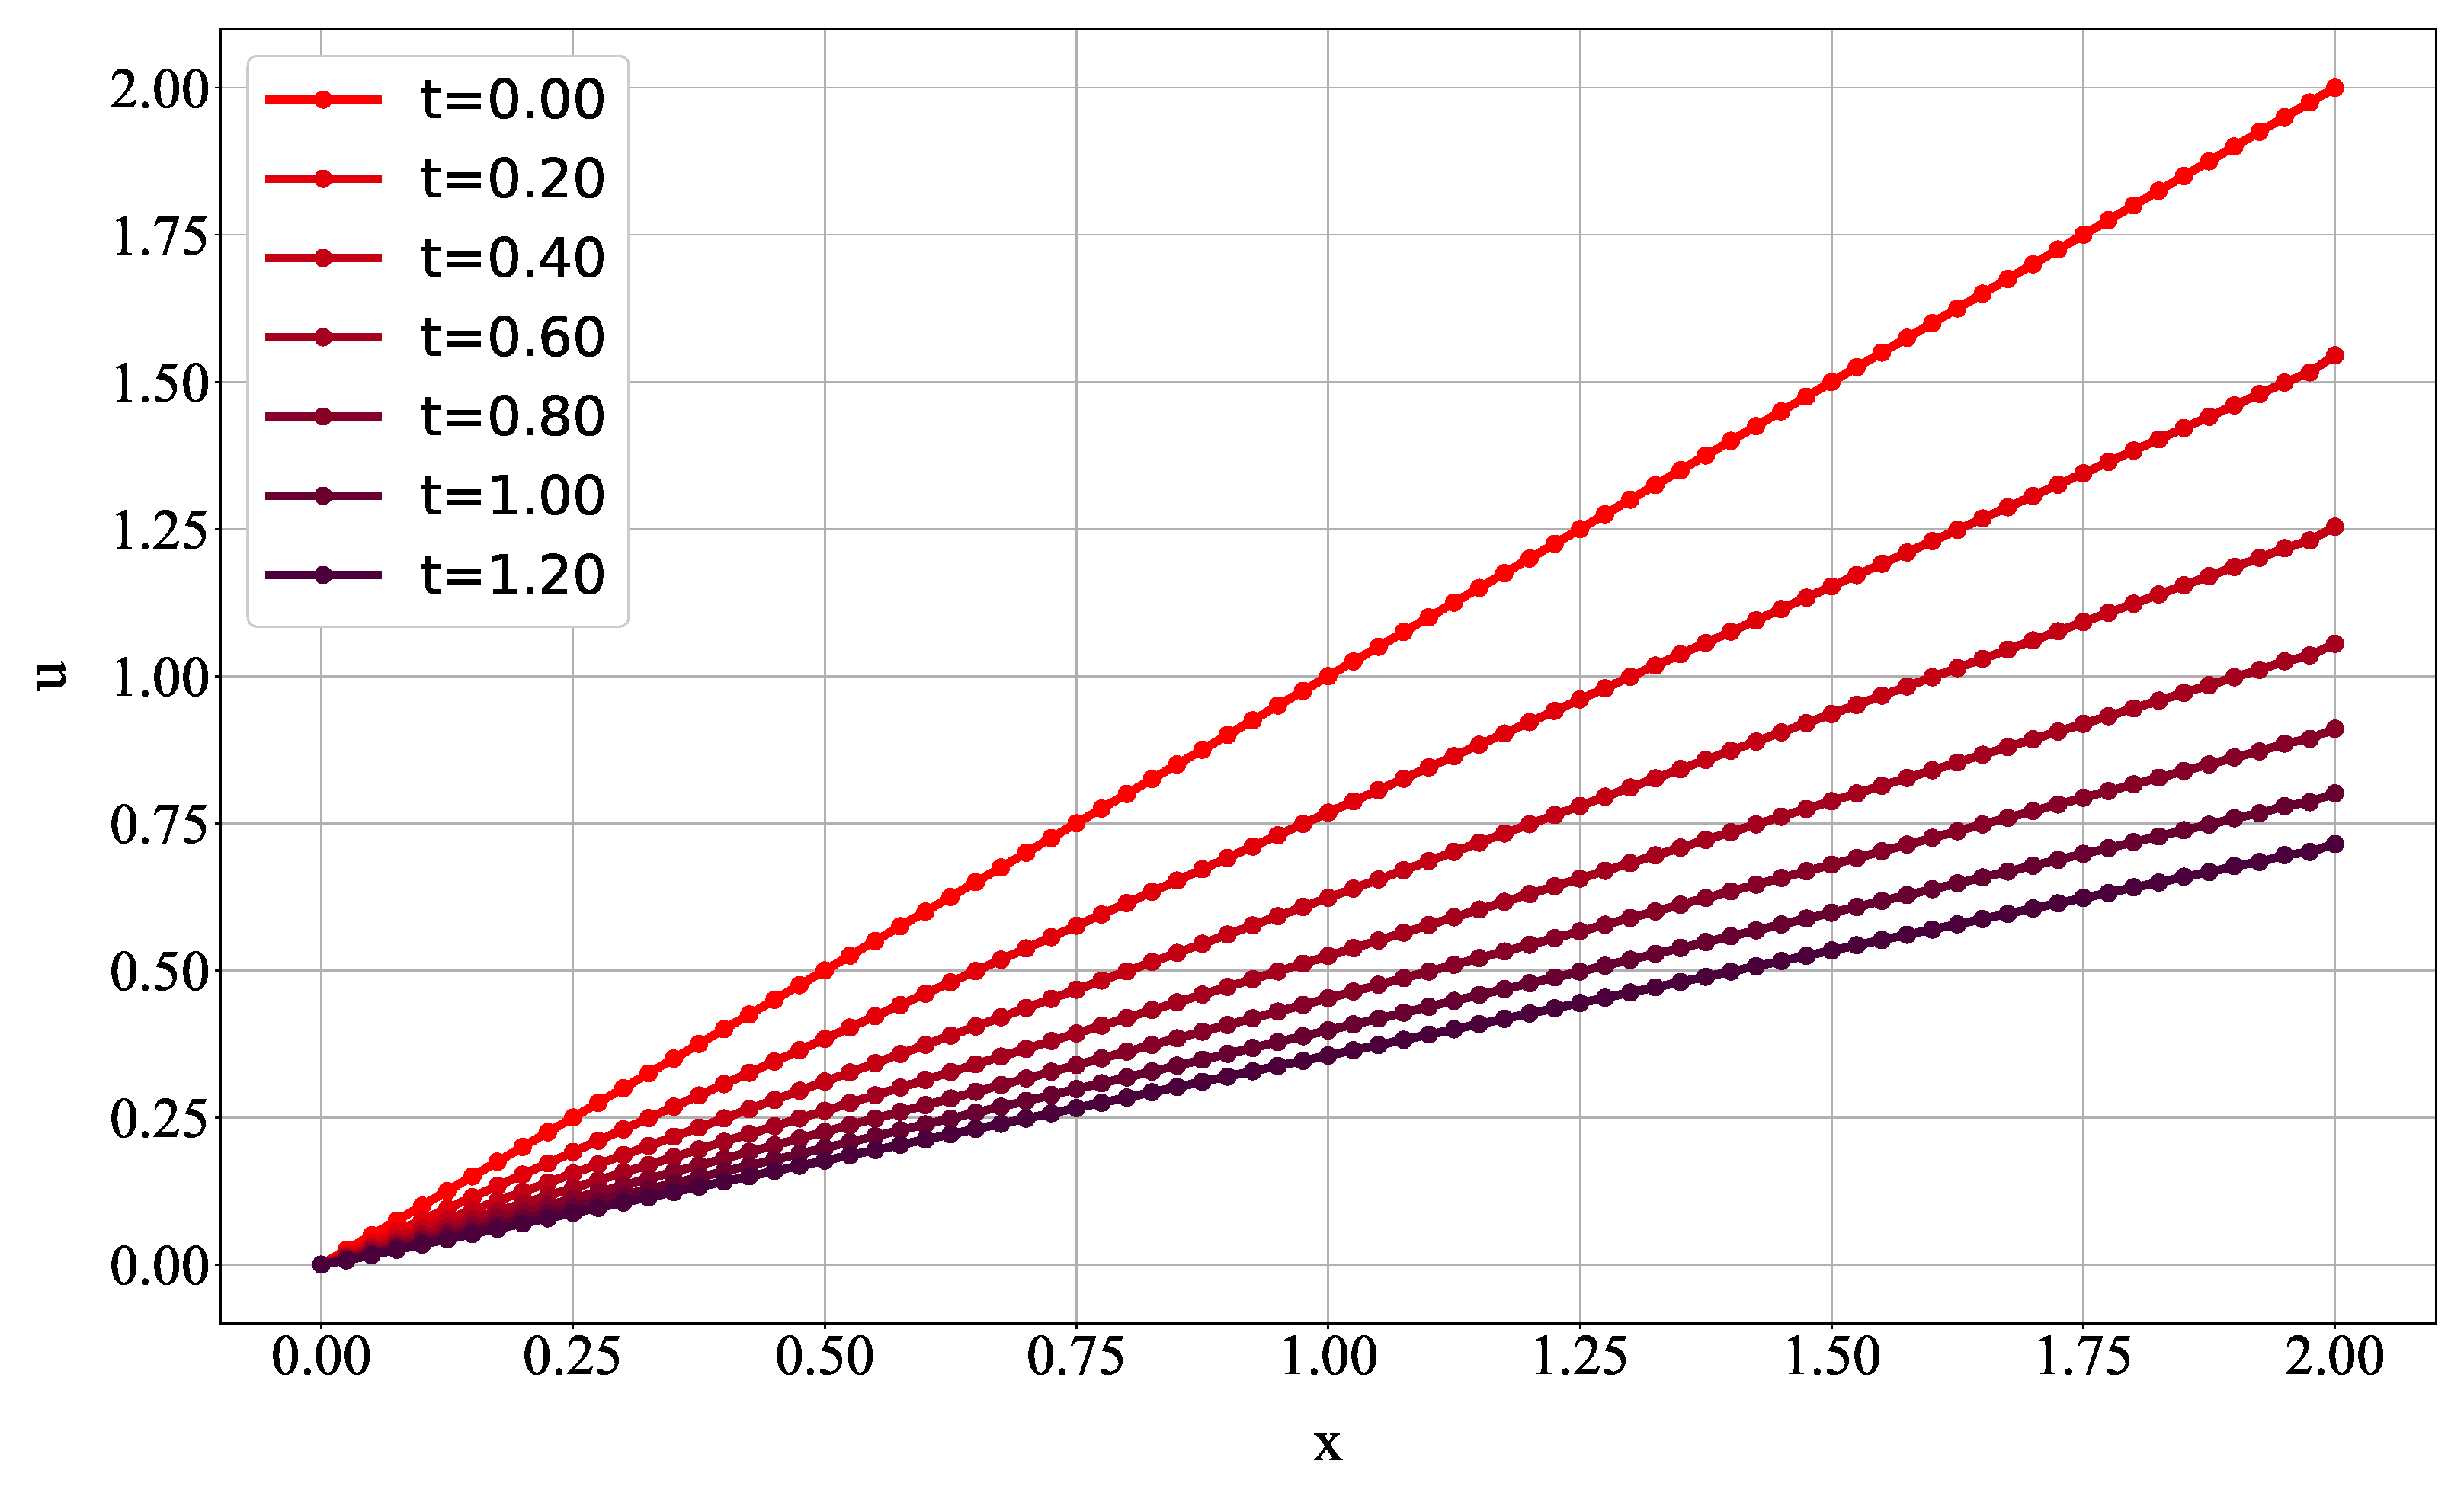
\includegraphics[width=\linewidth]{5.maccormack.cour05.f2025}
    \end{subfigure}
    
    \begin{subfigure}[t]{0.5\textwidth}
      \caption*{$\cour = 0.9,\ f_2,\ h = 0.050$}
      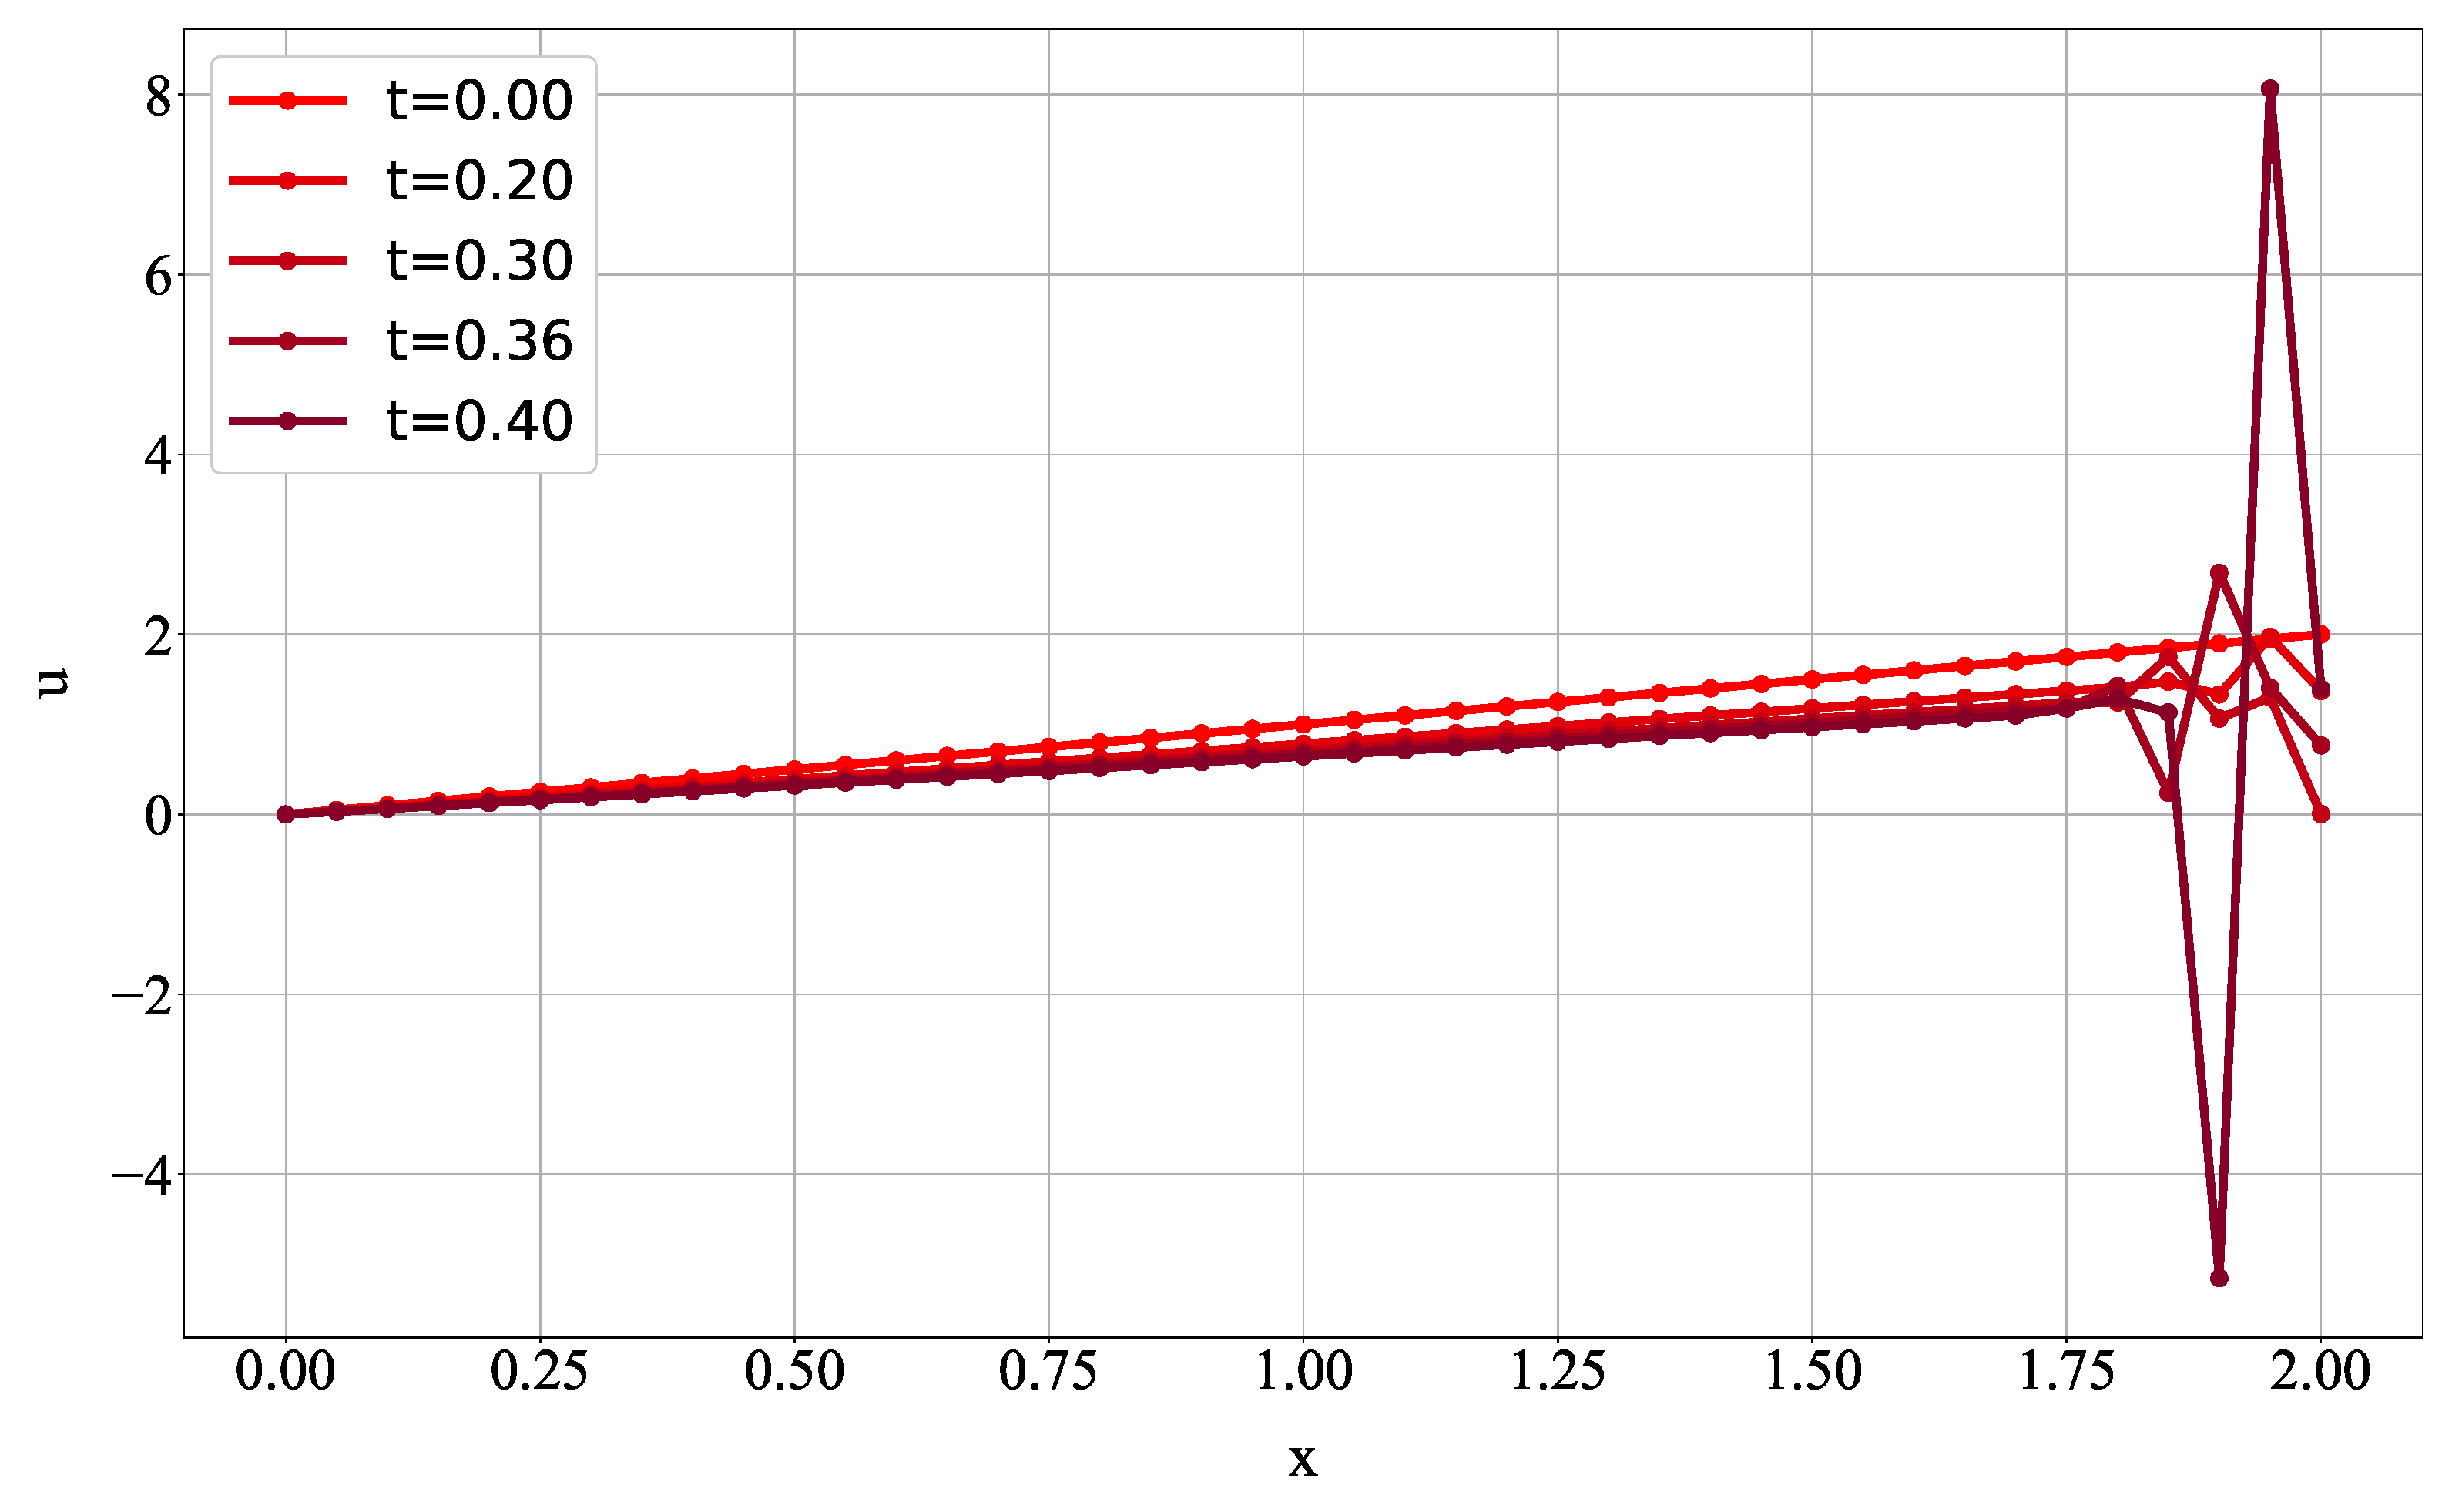
\includegraphics[width=\linewidth]{5.maccormack.cour09.f2050}
    \end{subfigure}
    ~
    \begin{subfigure}[t]{0.5\textwidth}
      \caption*{$\cour = 0.9,\ f_2,\ h = 0.025$}
      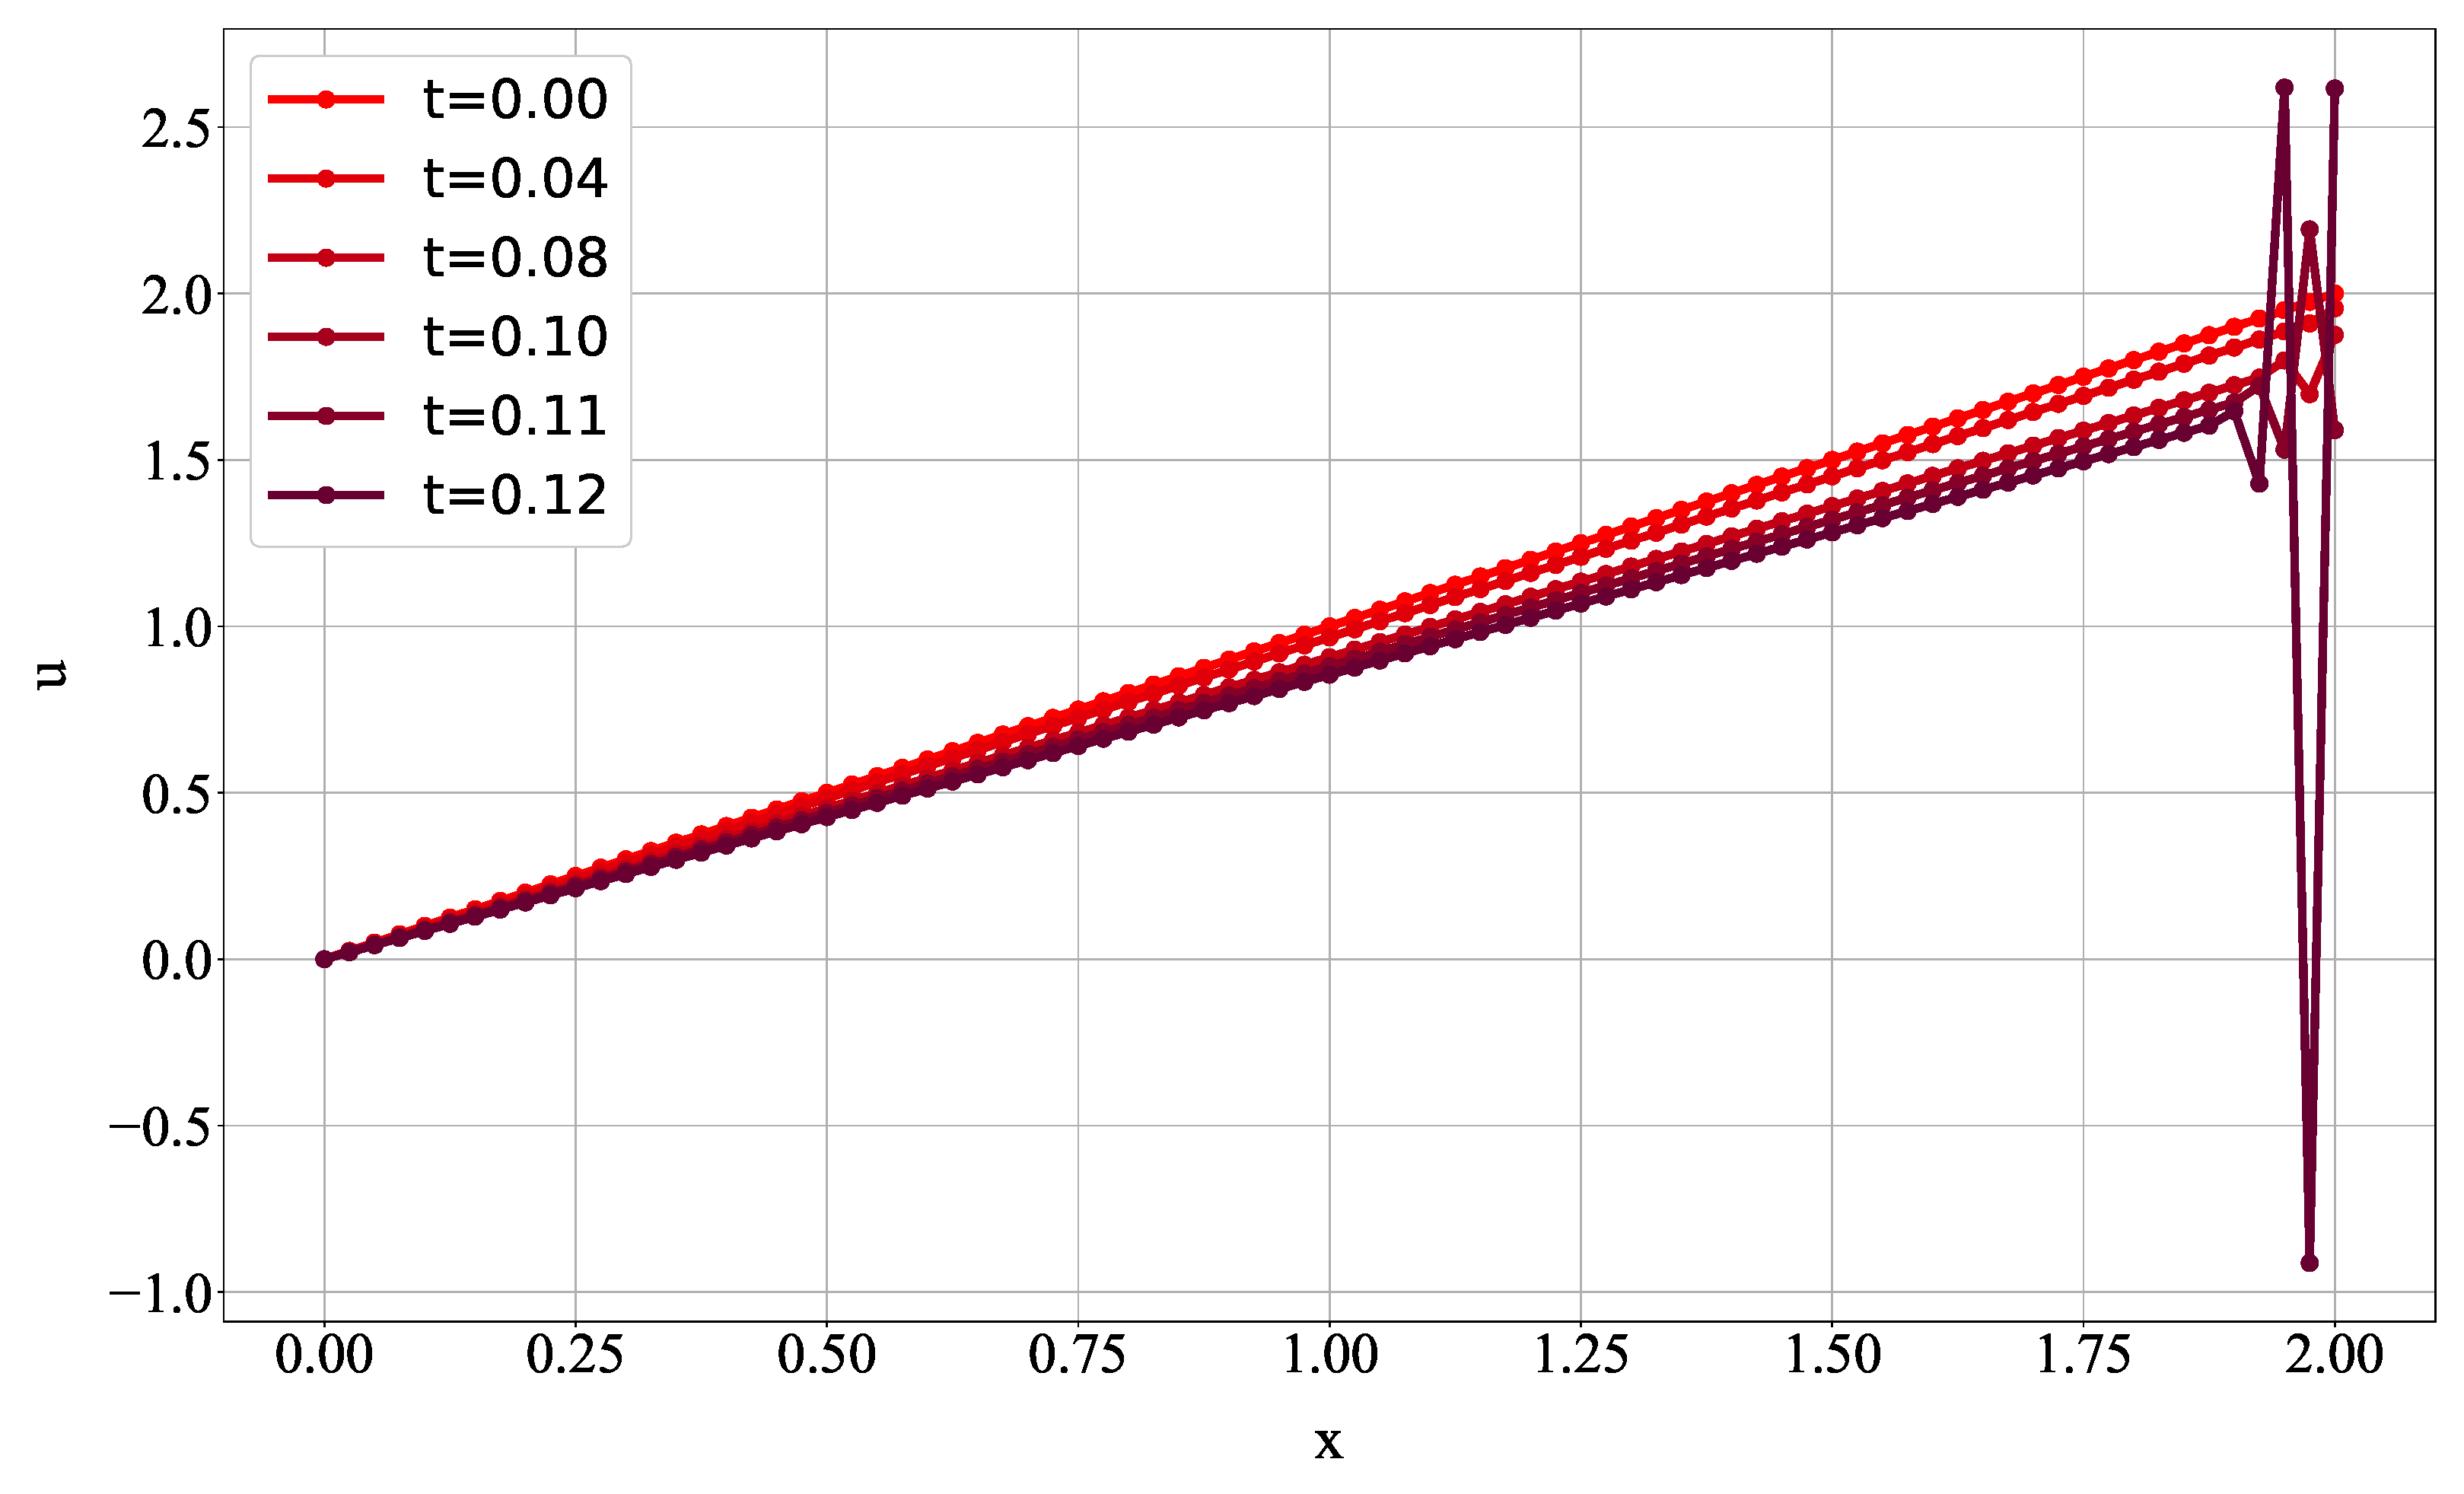
\includegraphics[width=\linewidth]{5.maccormack.cour09.f2025}
    \end{subfigure}
    \caption{"`МакКормак"'}
    \label{plot:maccormack}
  \end{figure}
  \fi
  
\section{Графики}
  \begin{table}[h!]
  \caption{"`Наивный"' (\ref{sec:silly})}
  \label{plot:silly}
  \begin{center}
    \begin{tabular}{c c c c}
      \toprule
      {$f$}                                       & $\sigma$ & $h_1$ & $h_2$\\
      \midrule
      \multirow{2}{*}{\vspace{\myvspaceOne}$f_1$} & $0.5$    & 
        \raisebox{-0.5\totalheight}{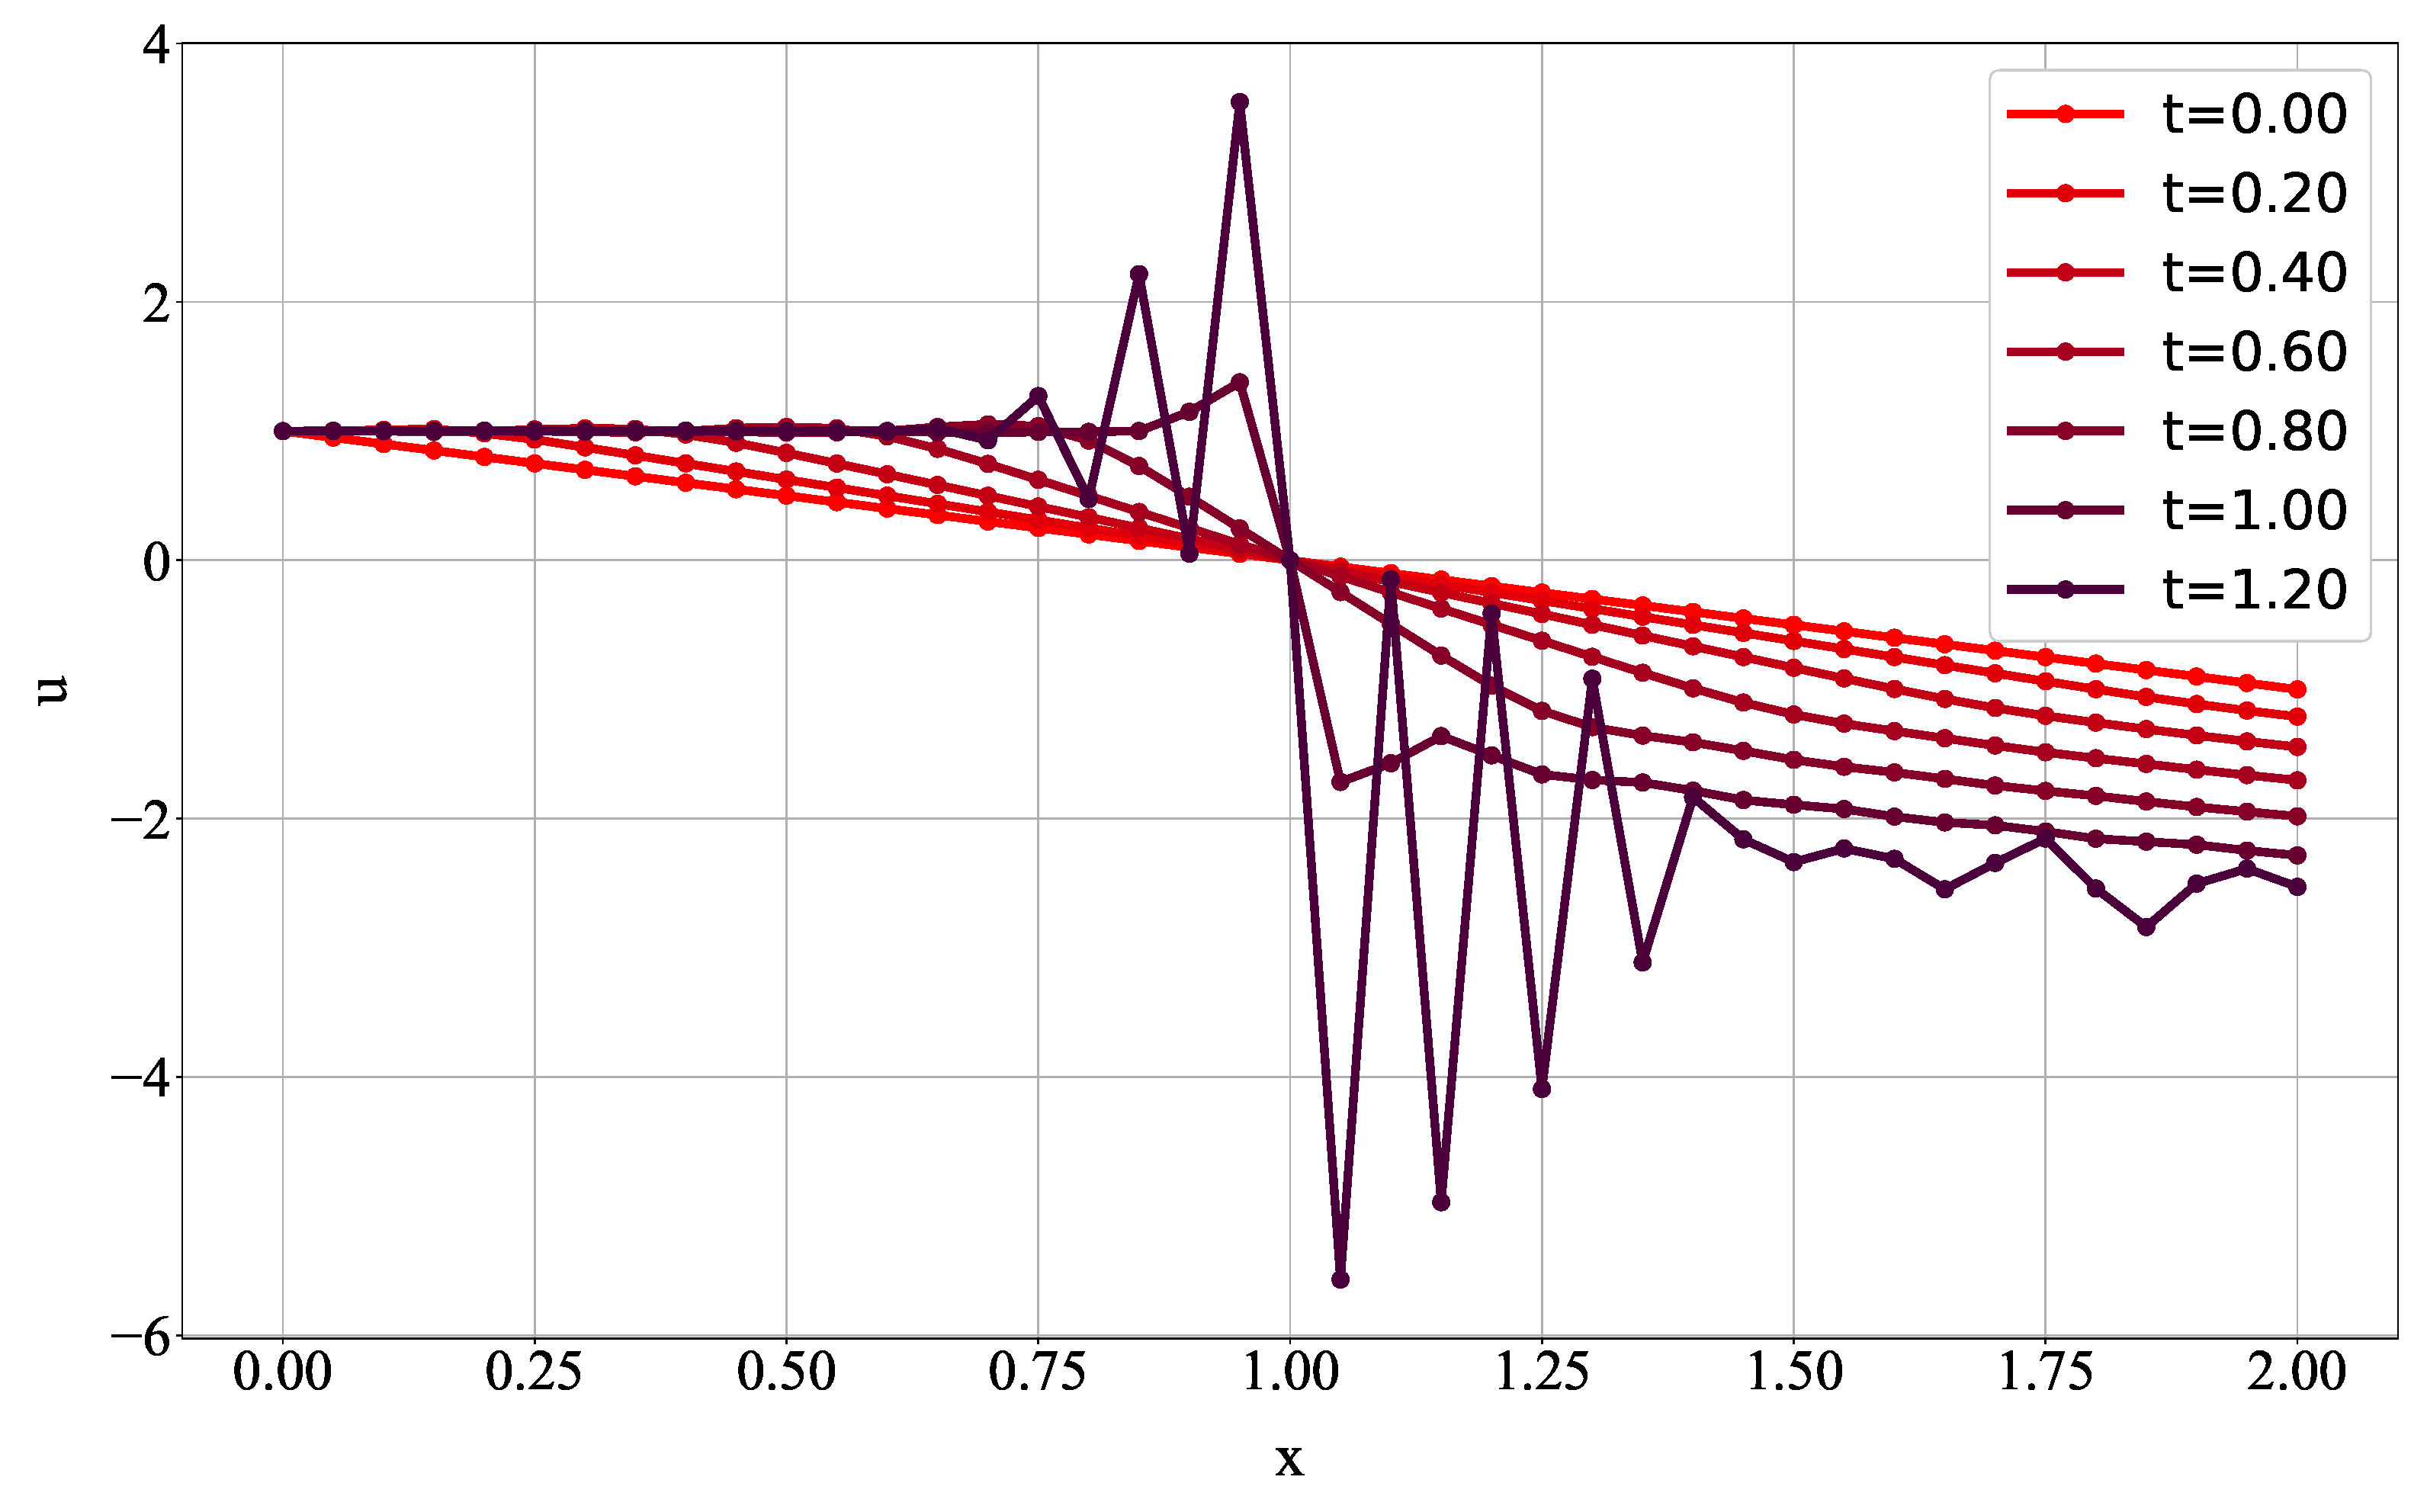
\includegraphics[width=0.425\linewidth]{1.silly.cour05.f1050}} &
        \raisebox{-0.5\totalheight}{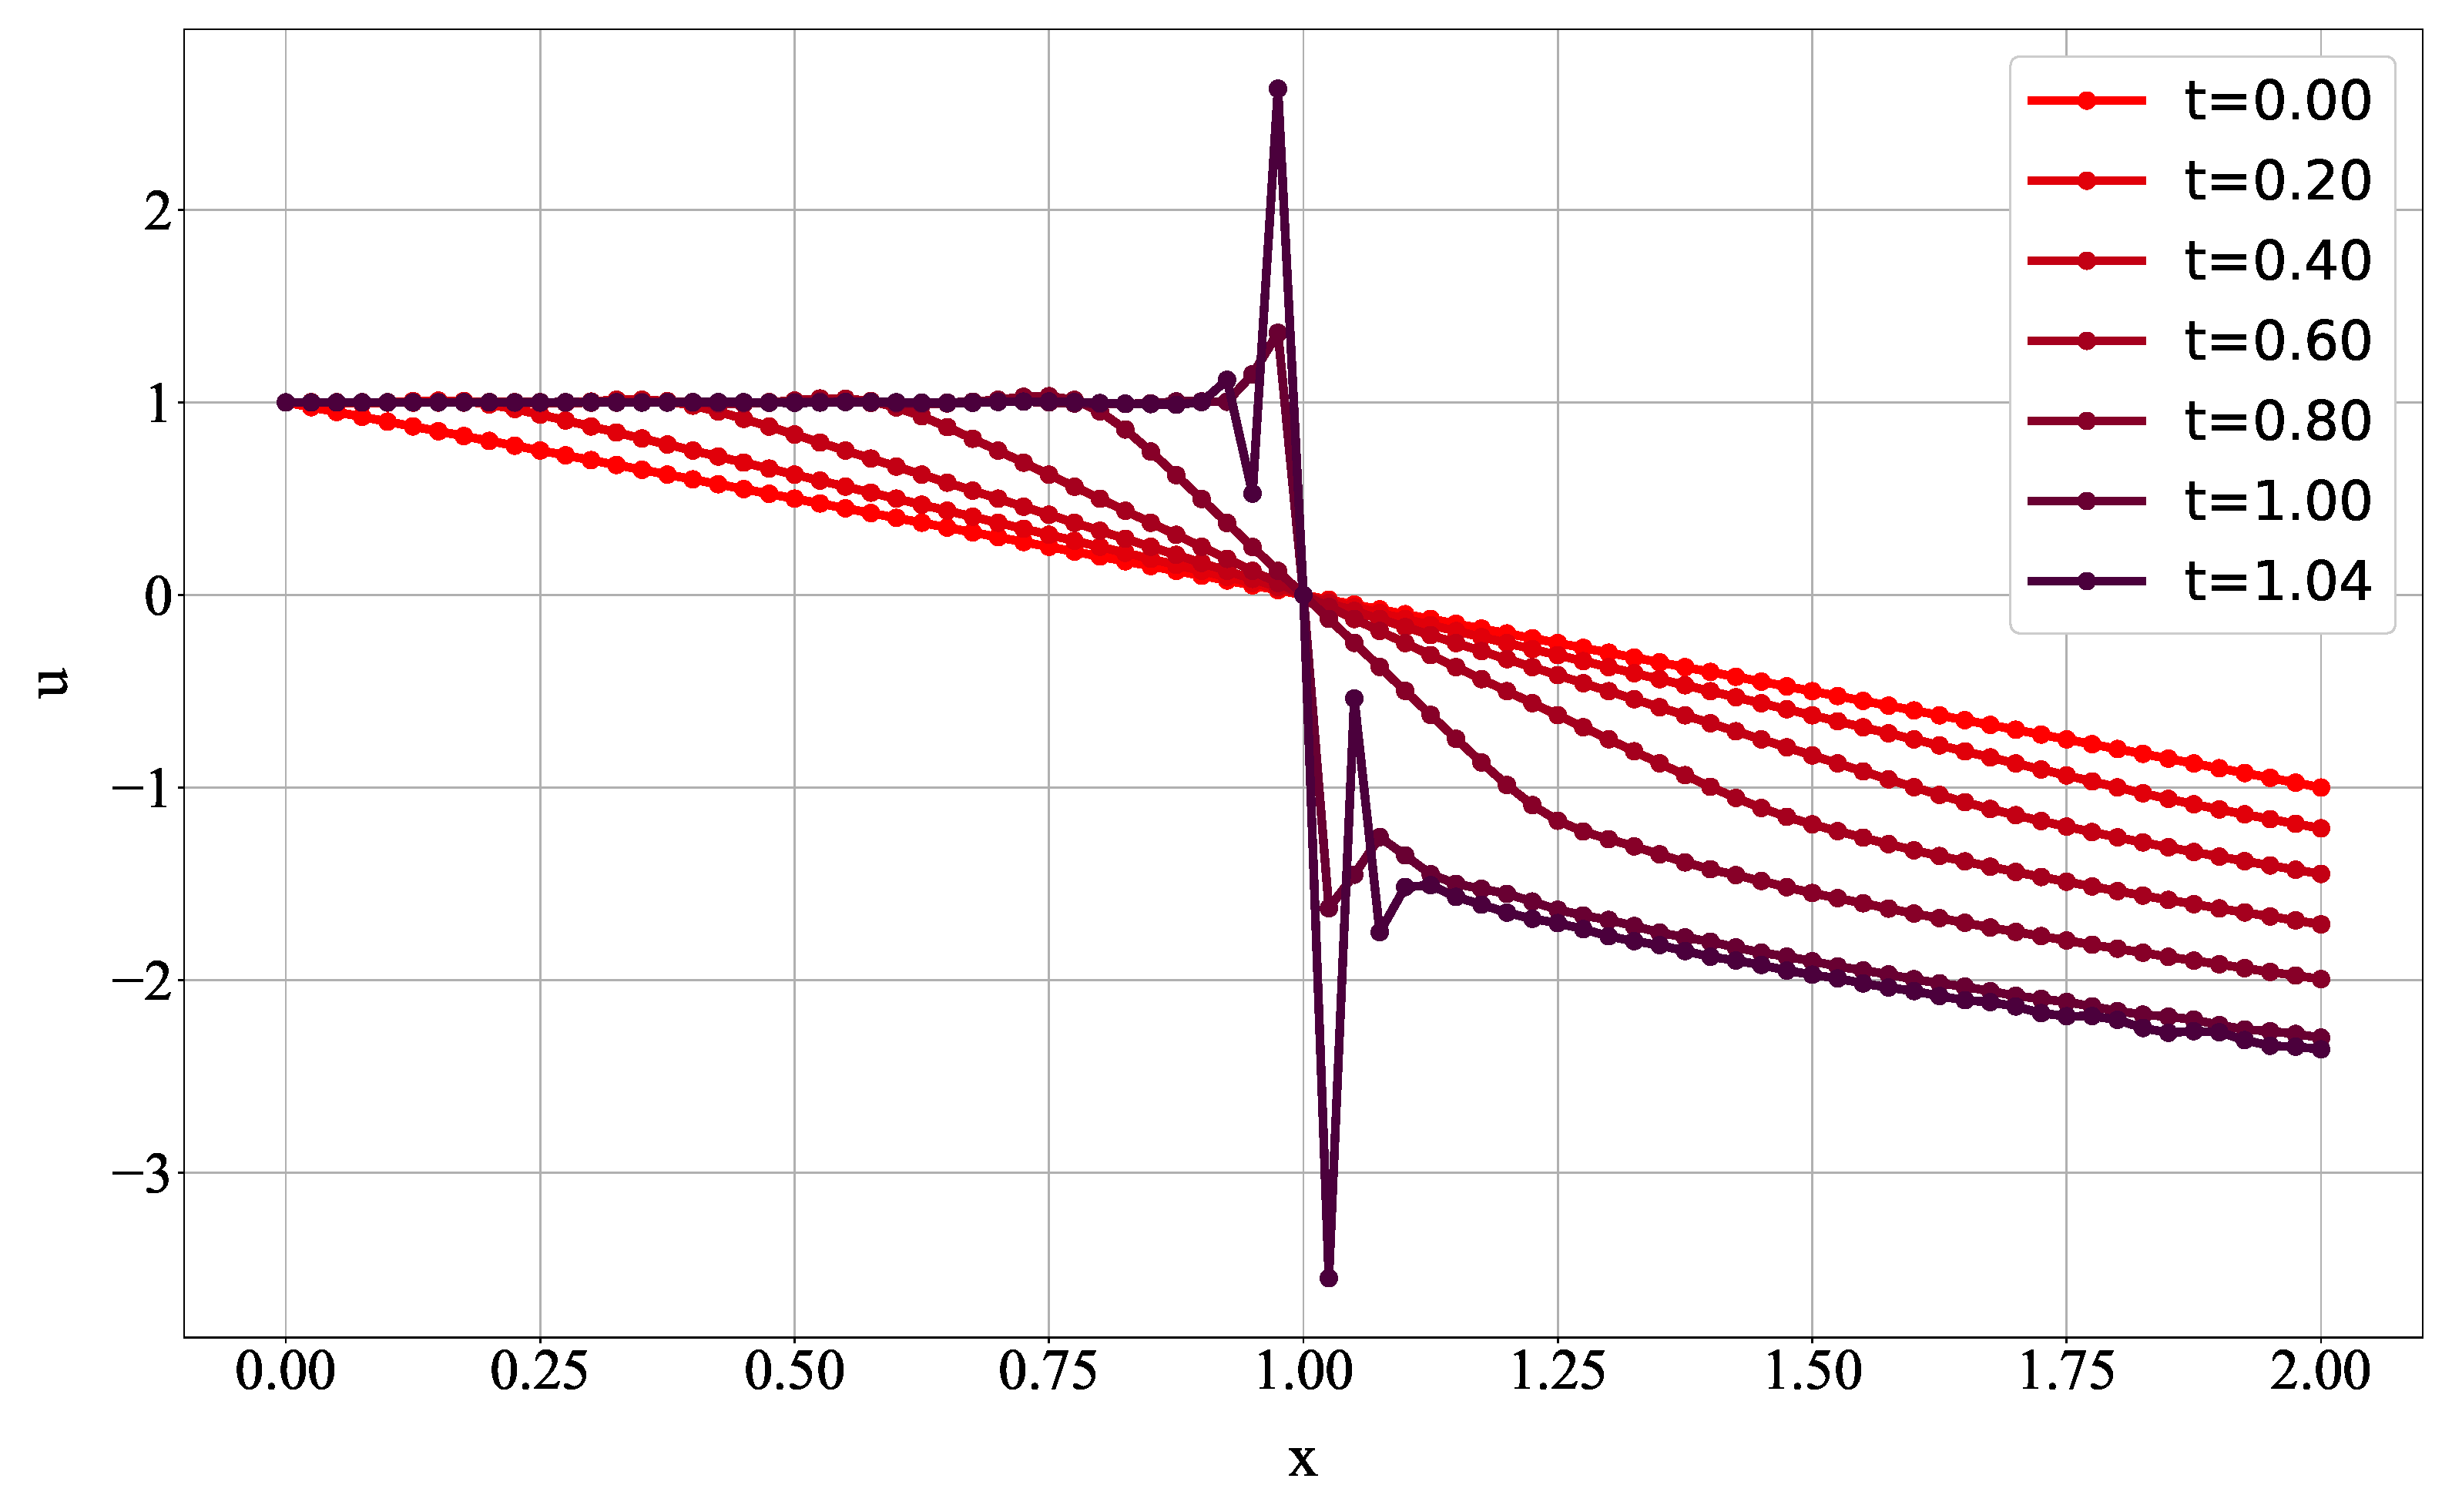
\includegraphics[width=0.425\linewidth]{1.silly.cour05.f1025}}\\
      %\cmidrule{3-4}
      {}                                          & $0.9$    &
        \raisebox{-0.5\totalheight}{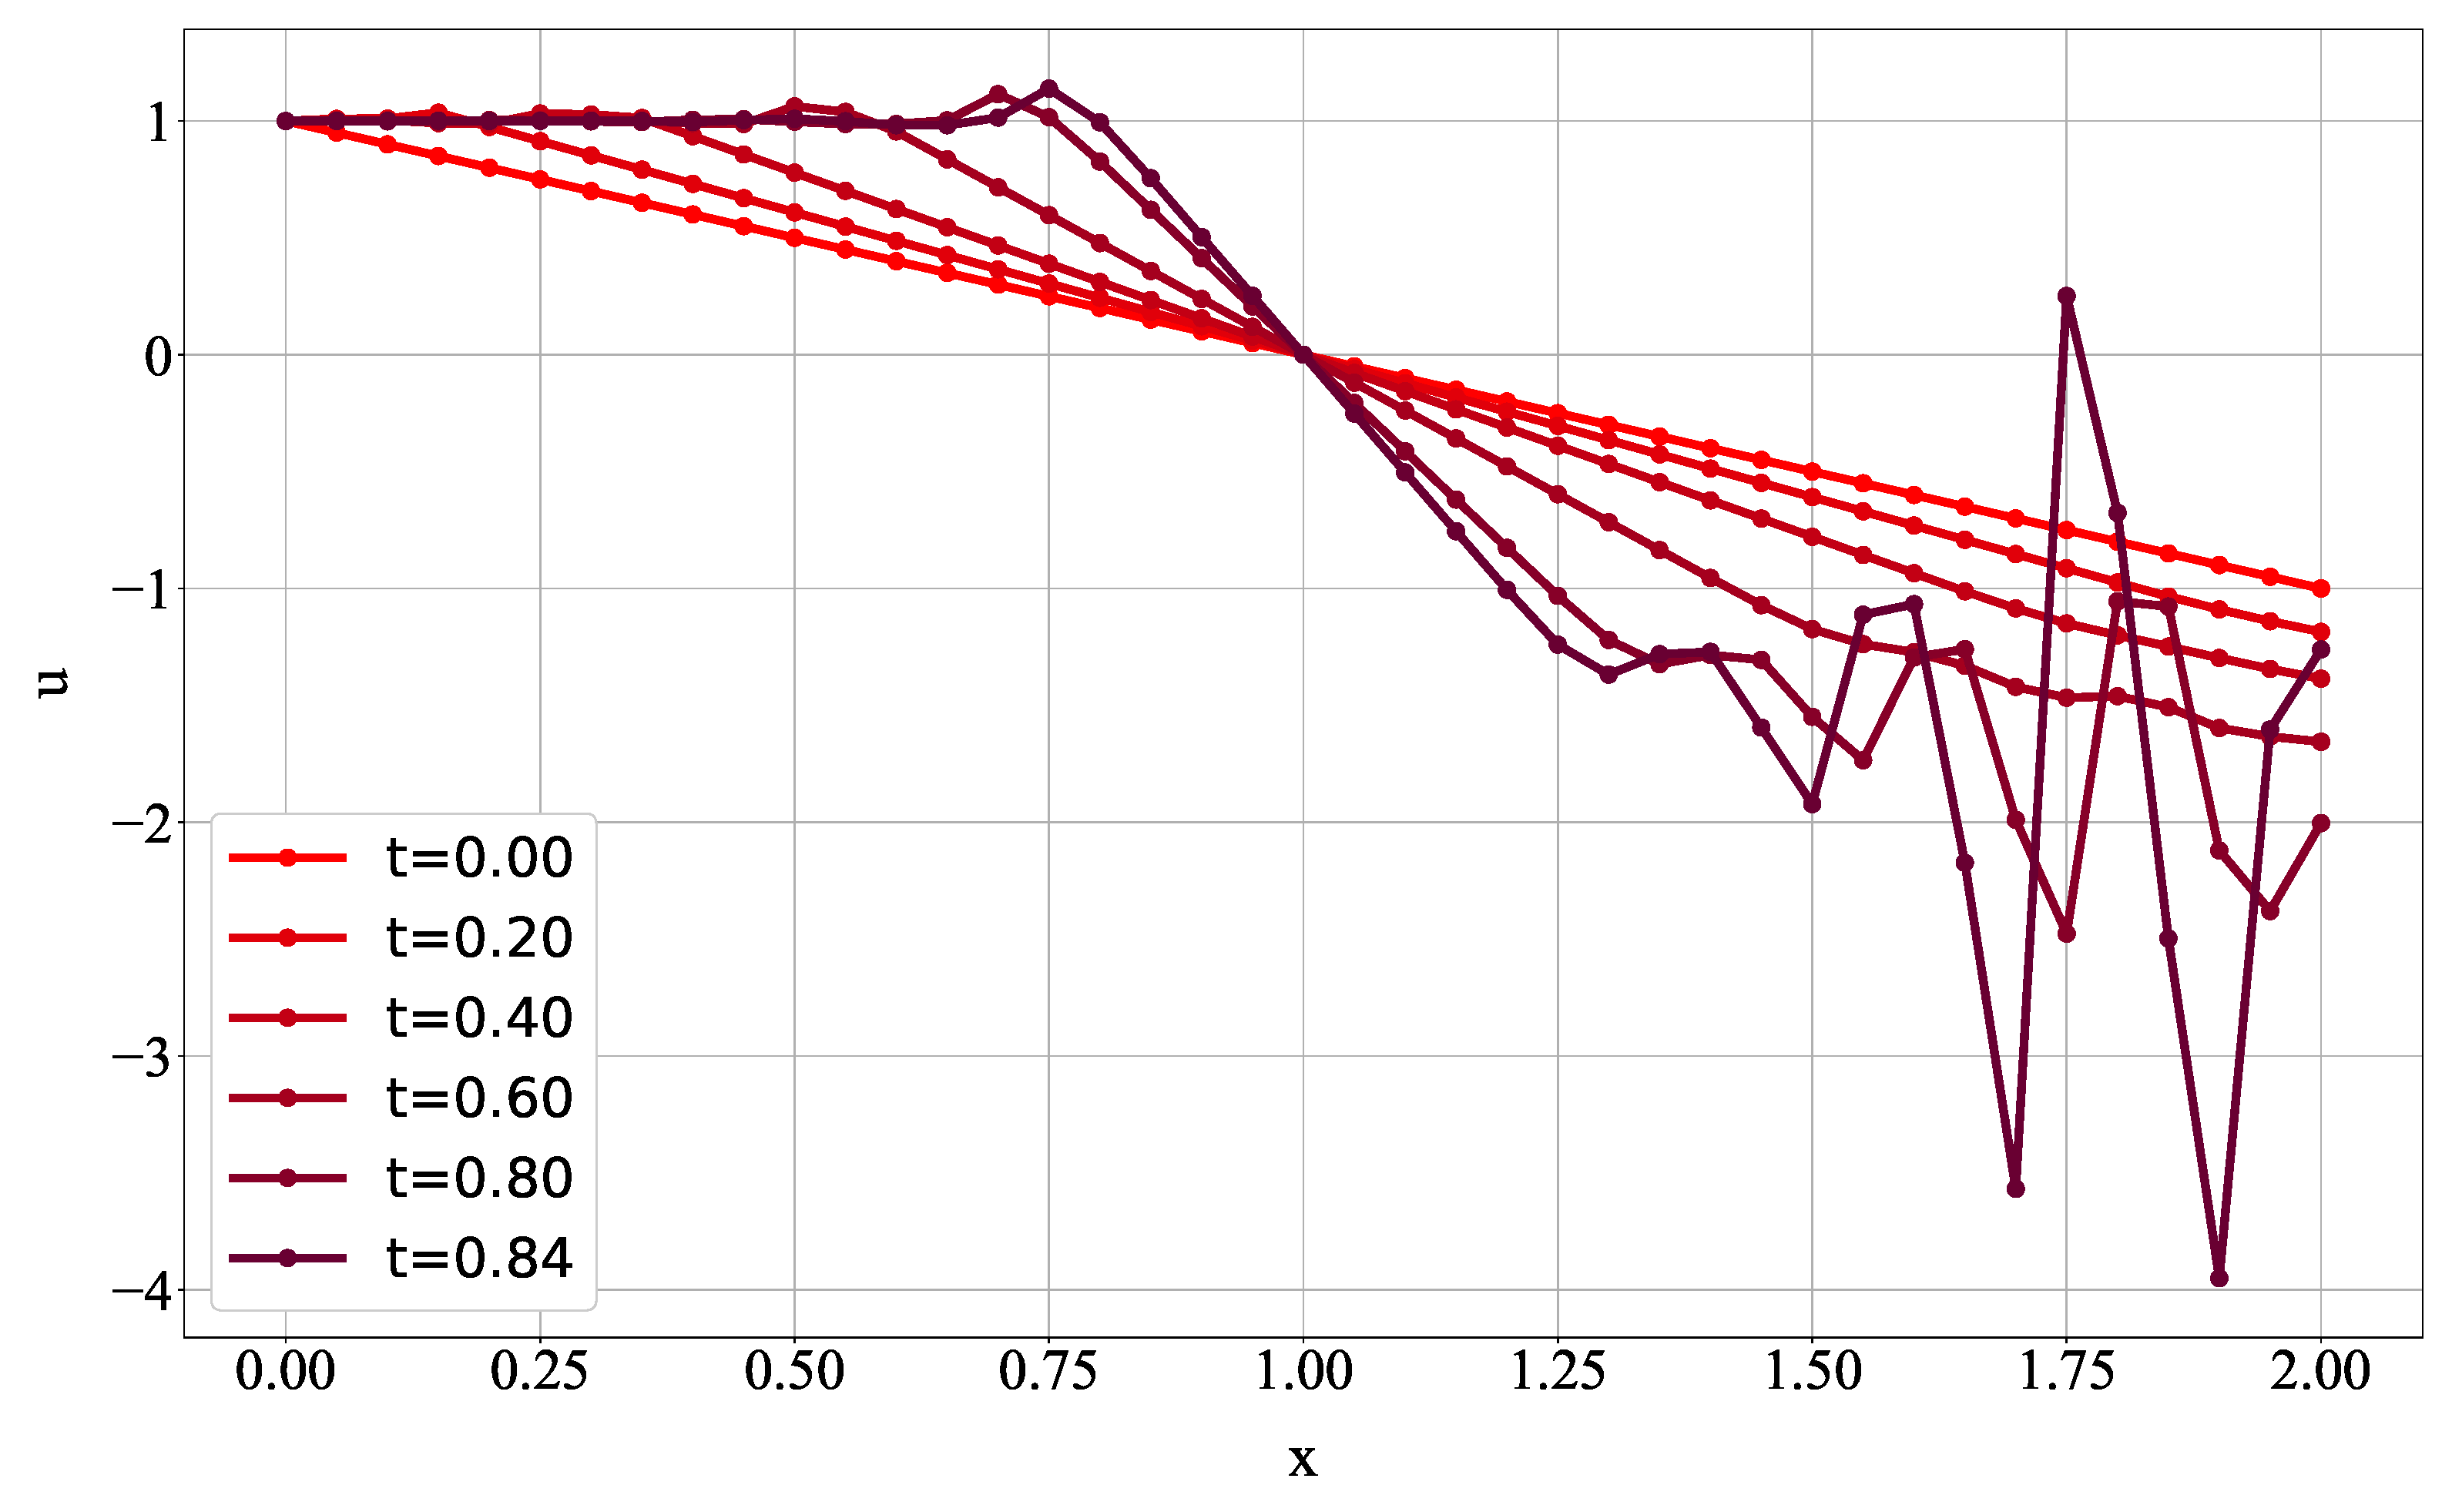
\includegraphics[width=0.425\linewidth]{1.silly.cour09.f1050}} & 
        \raisebox{-0.5\totalheight}{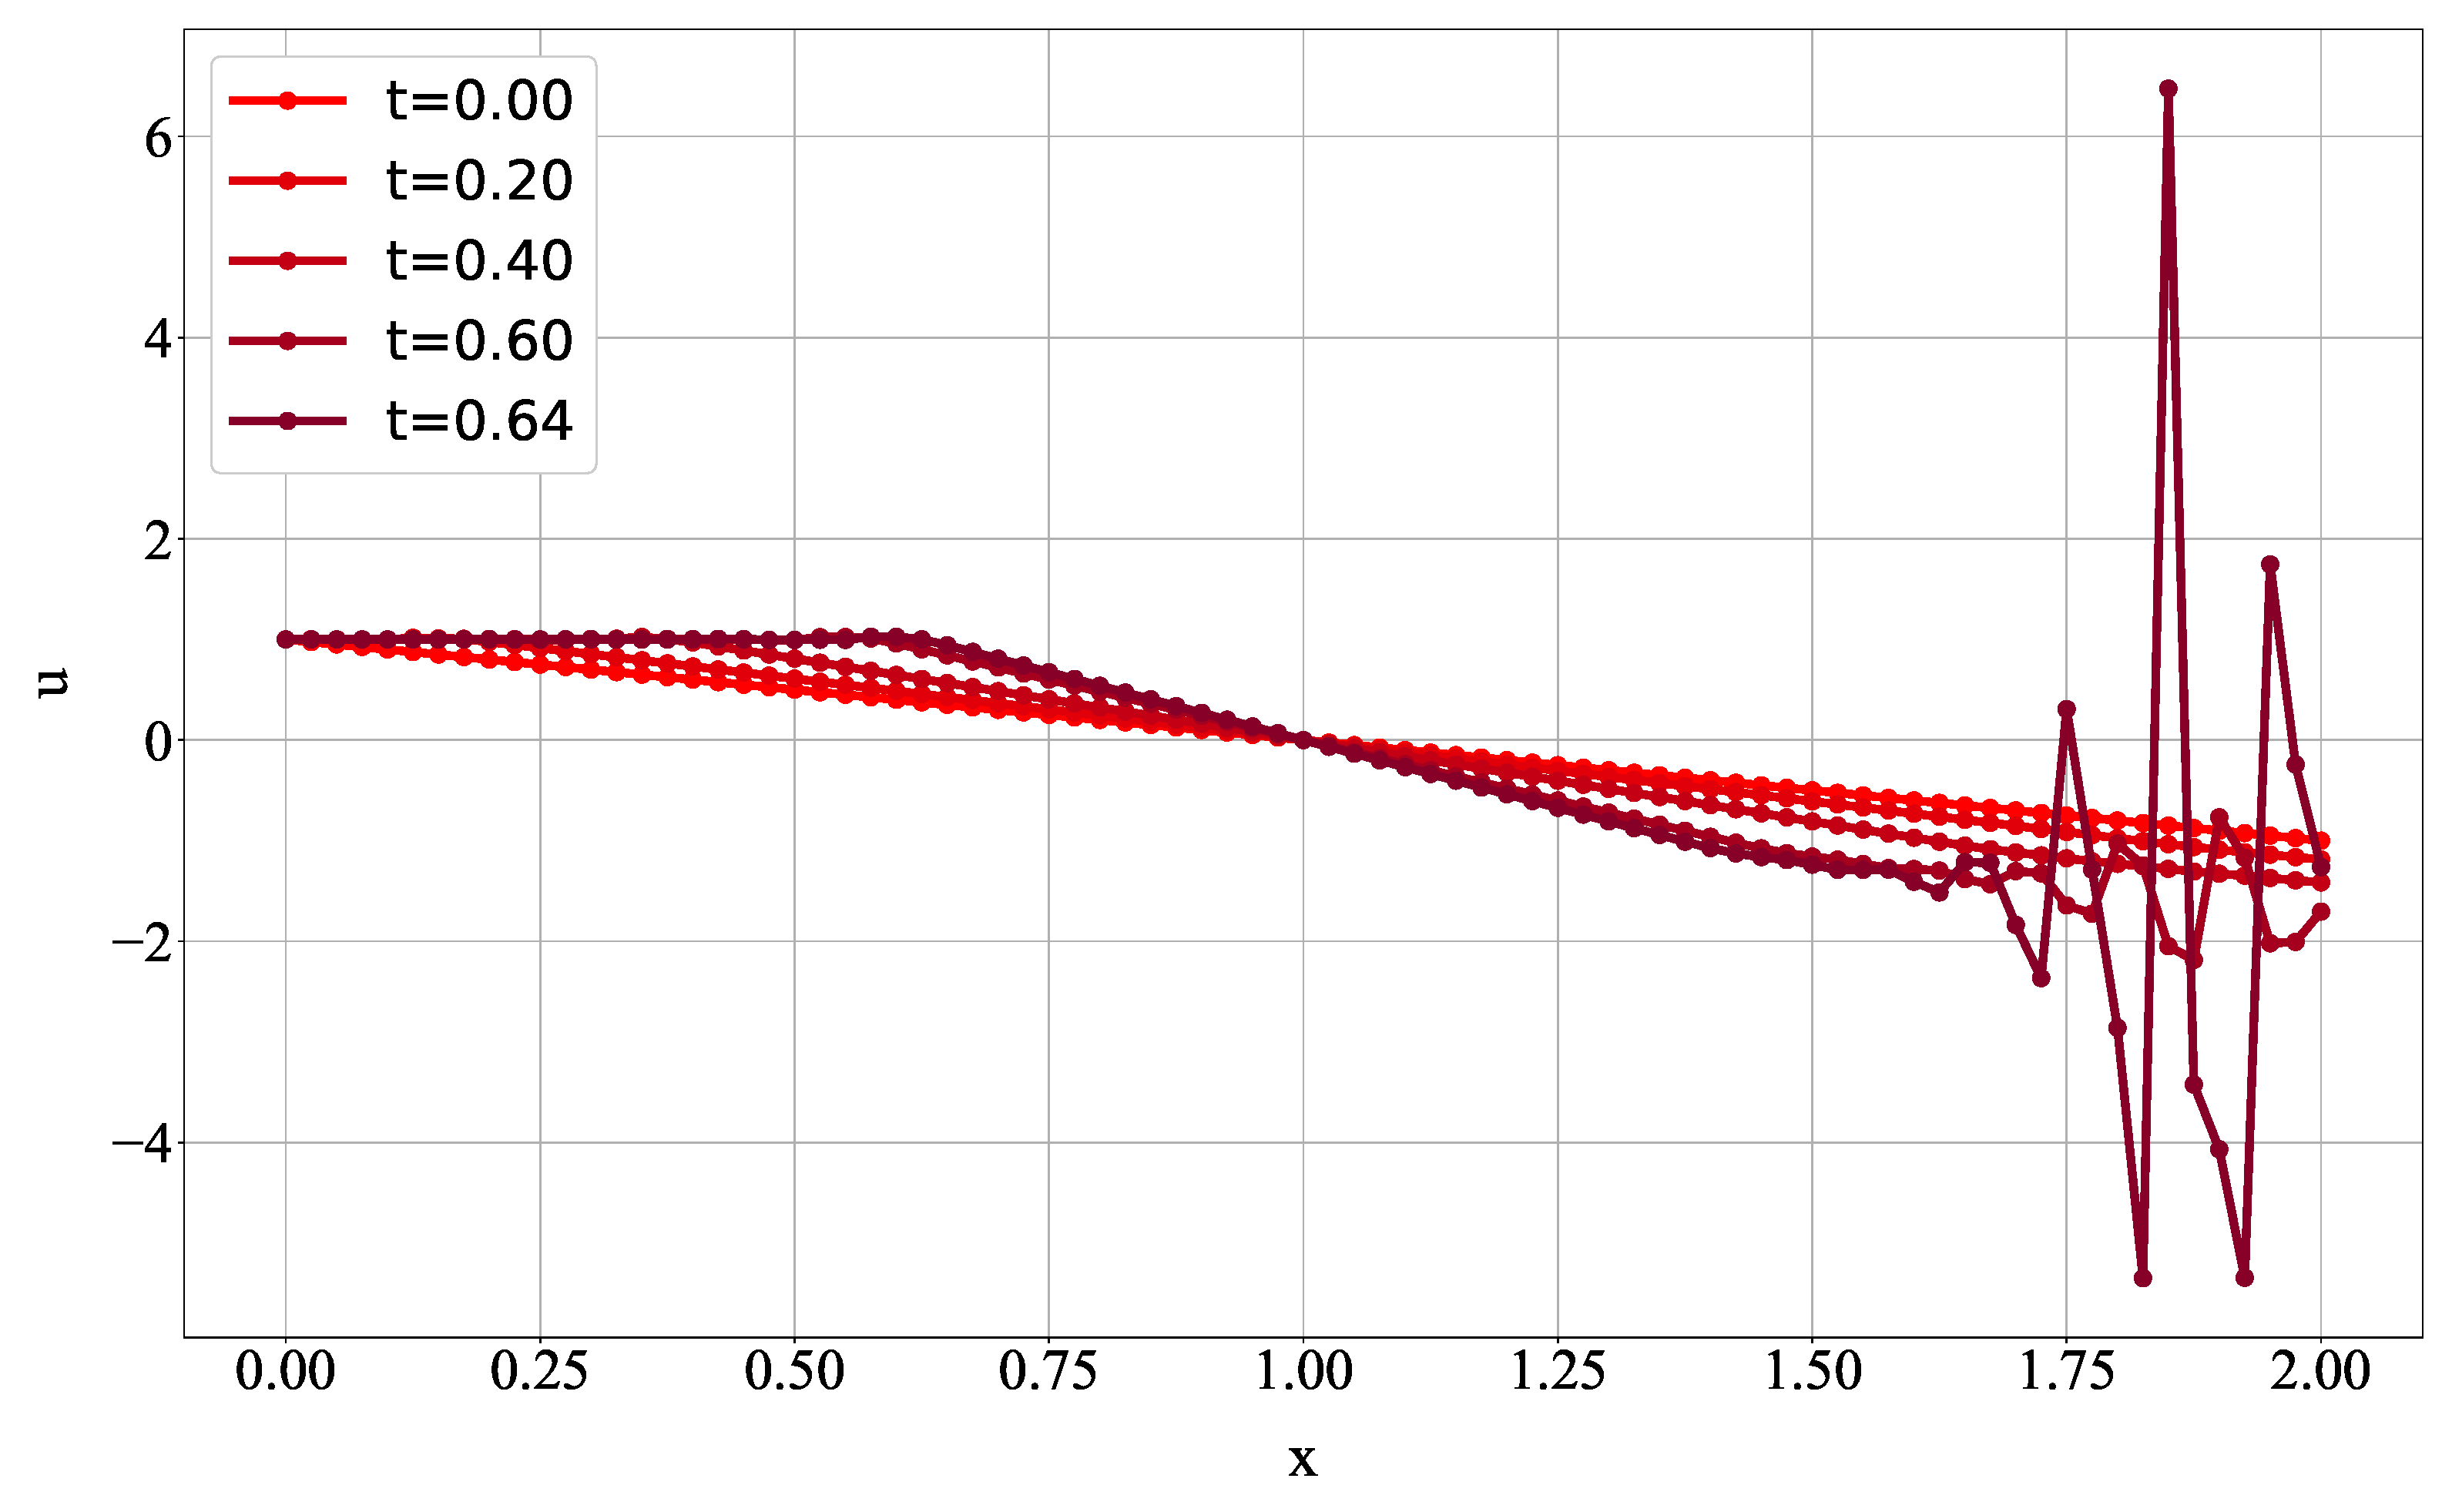
\includegraphics[width=0.425\linewidth]{1.silly.cour09.f1025}}\\
      \midrule
      \multirow{2}{*}{\vspace{\myvspaceOne}$f_2$} & $0.5$    &
        \raisebox{-0.5\totalheight}{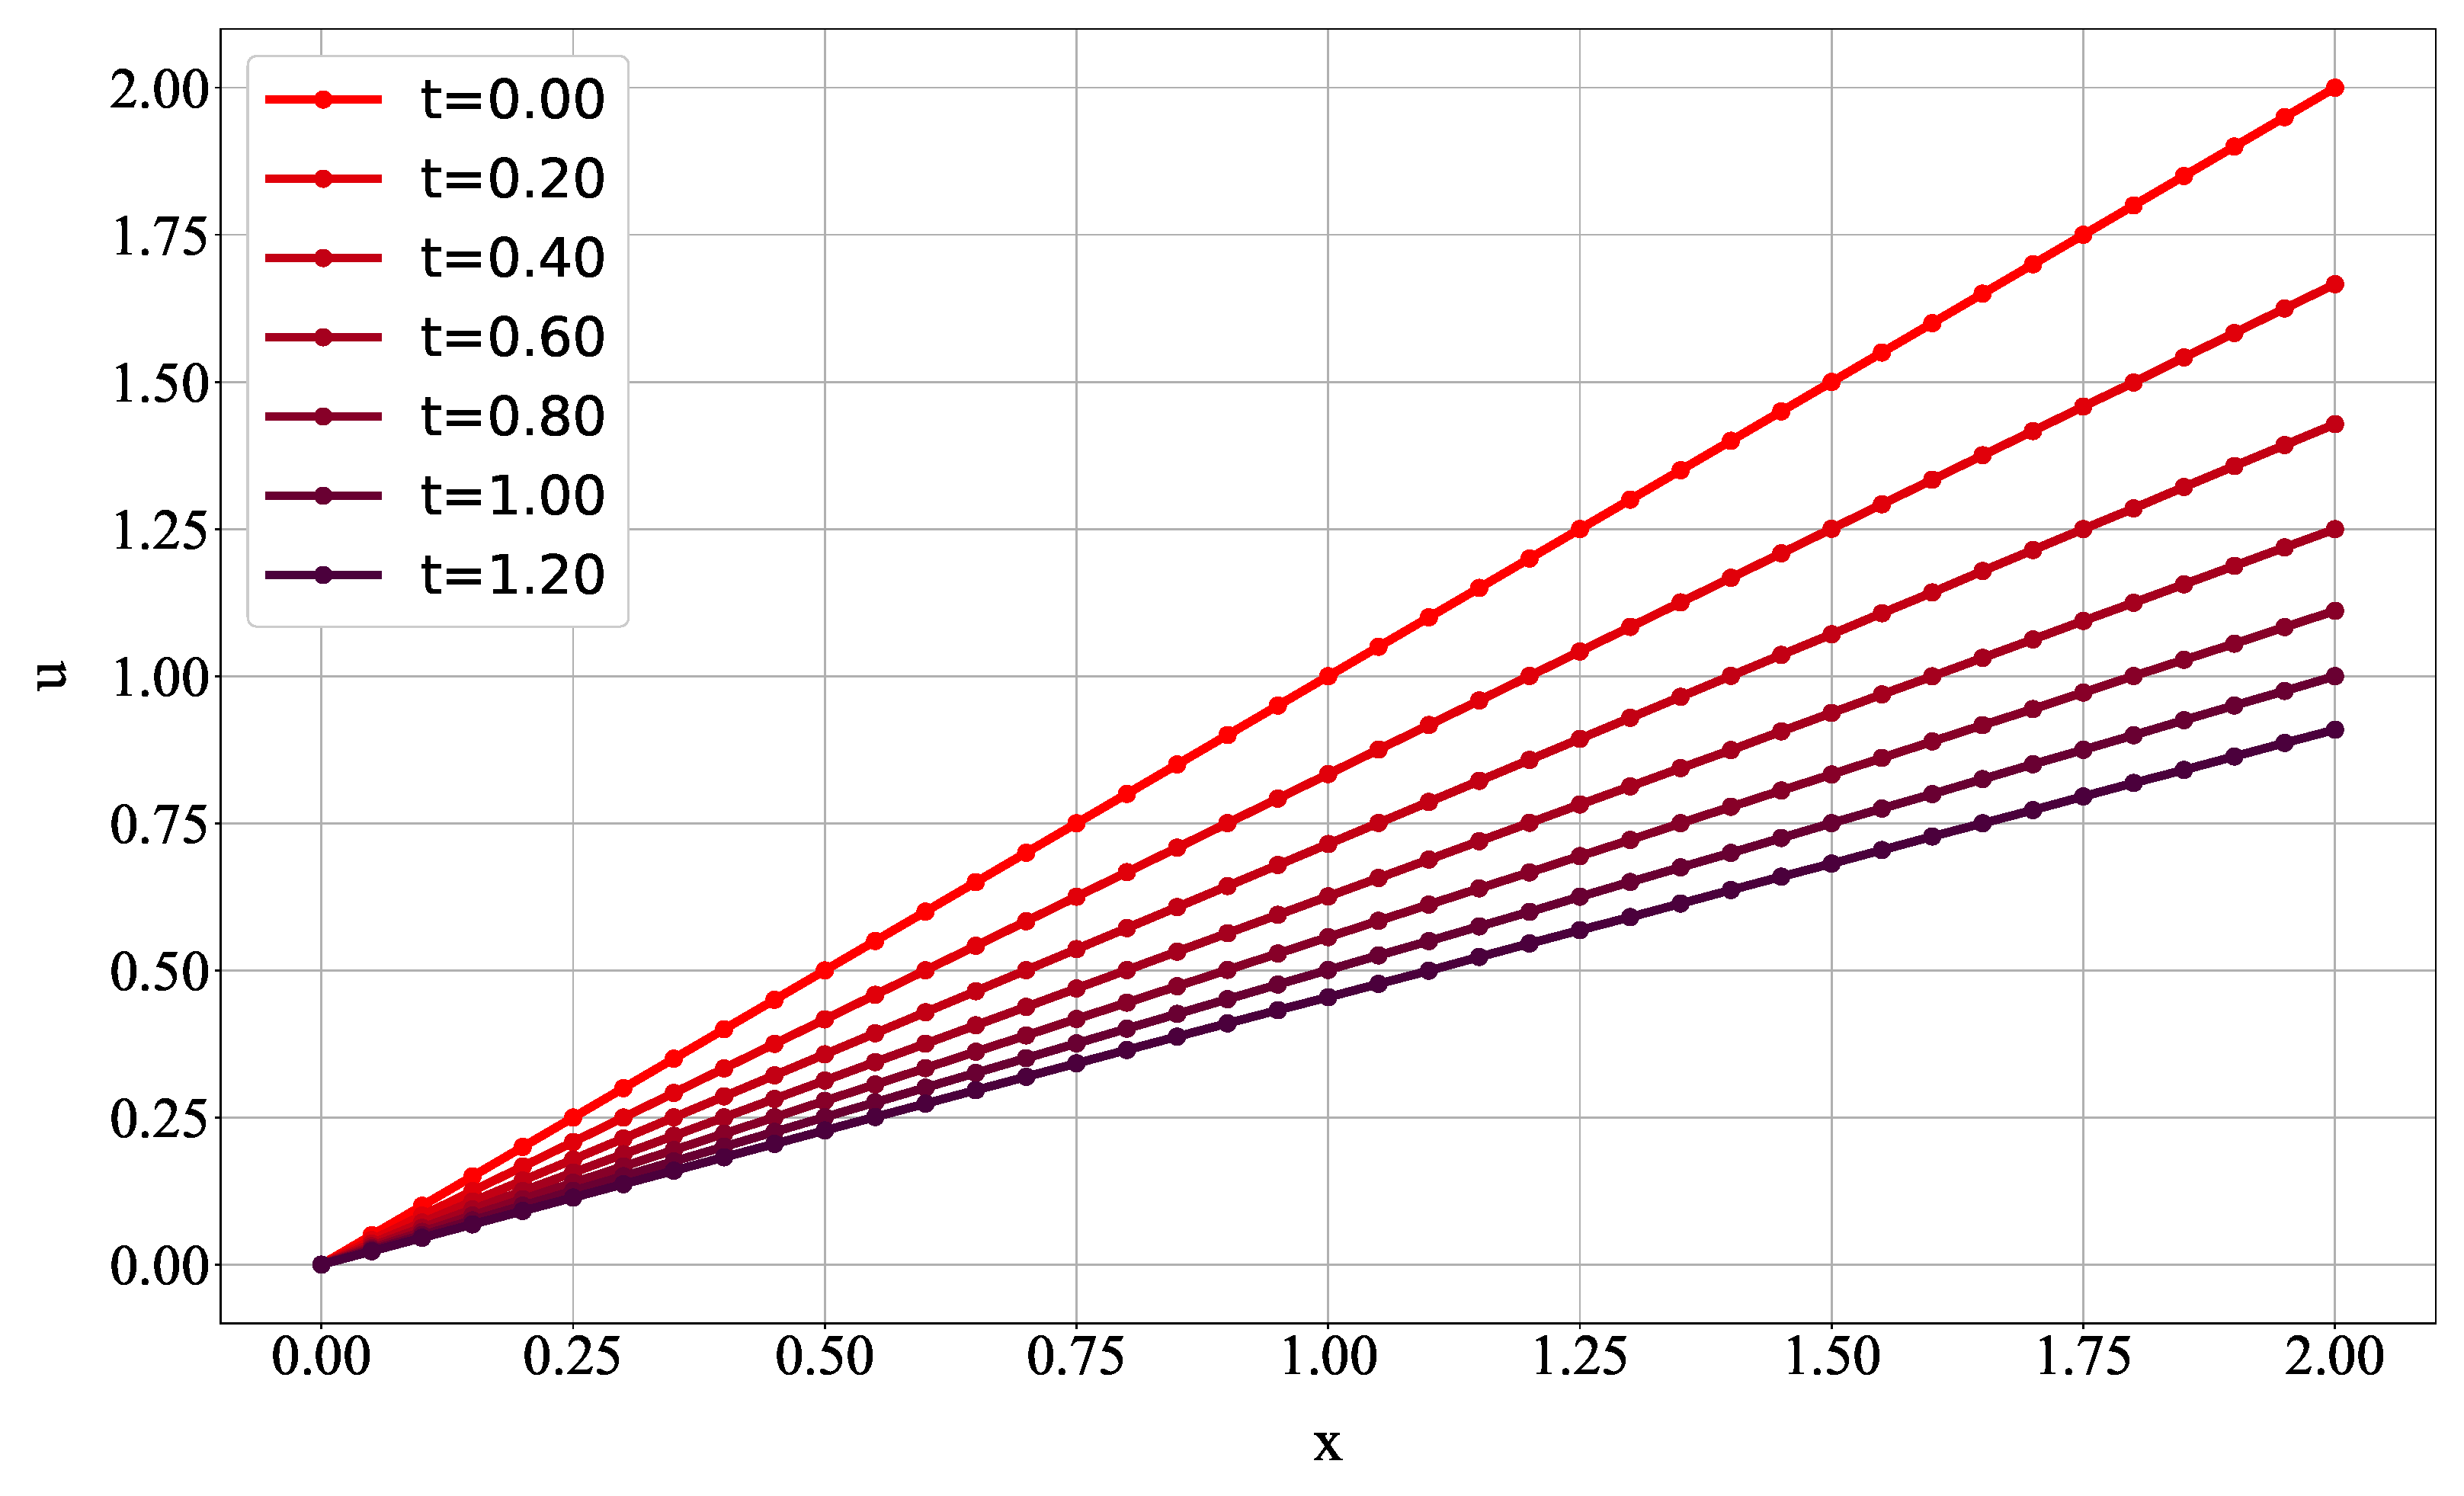
\includegraphics[width=0.425\linewidth]{1.silly.cour05.f2050}} &
        \raisebox{-0.5\totalheight}{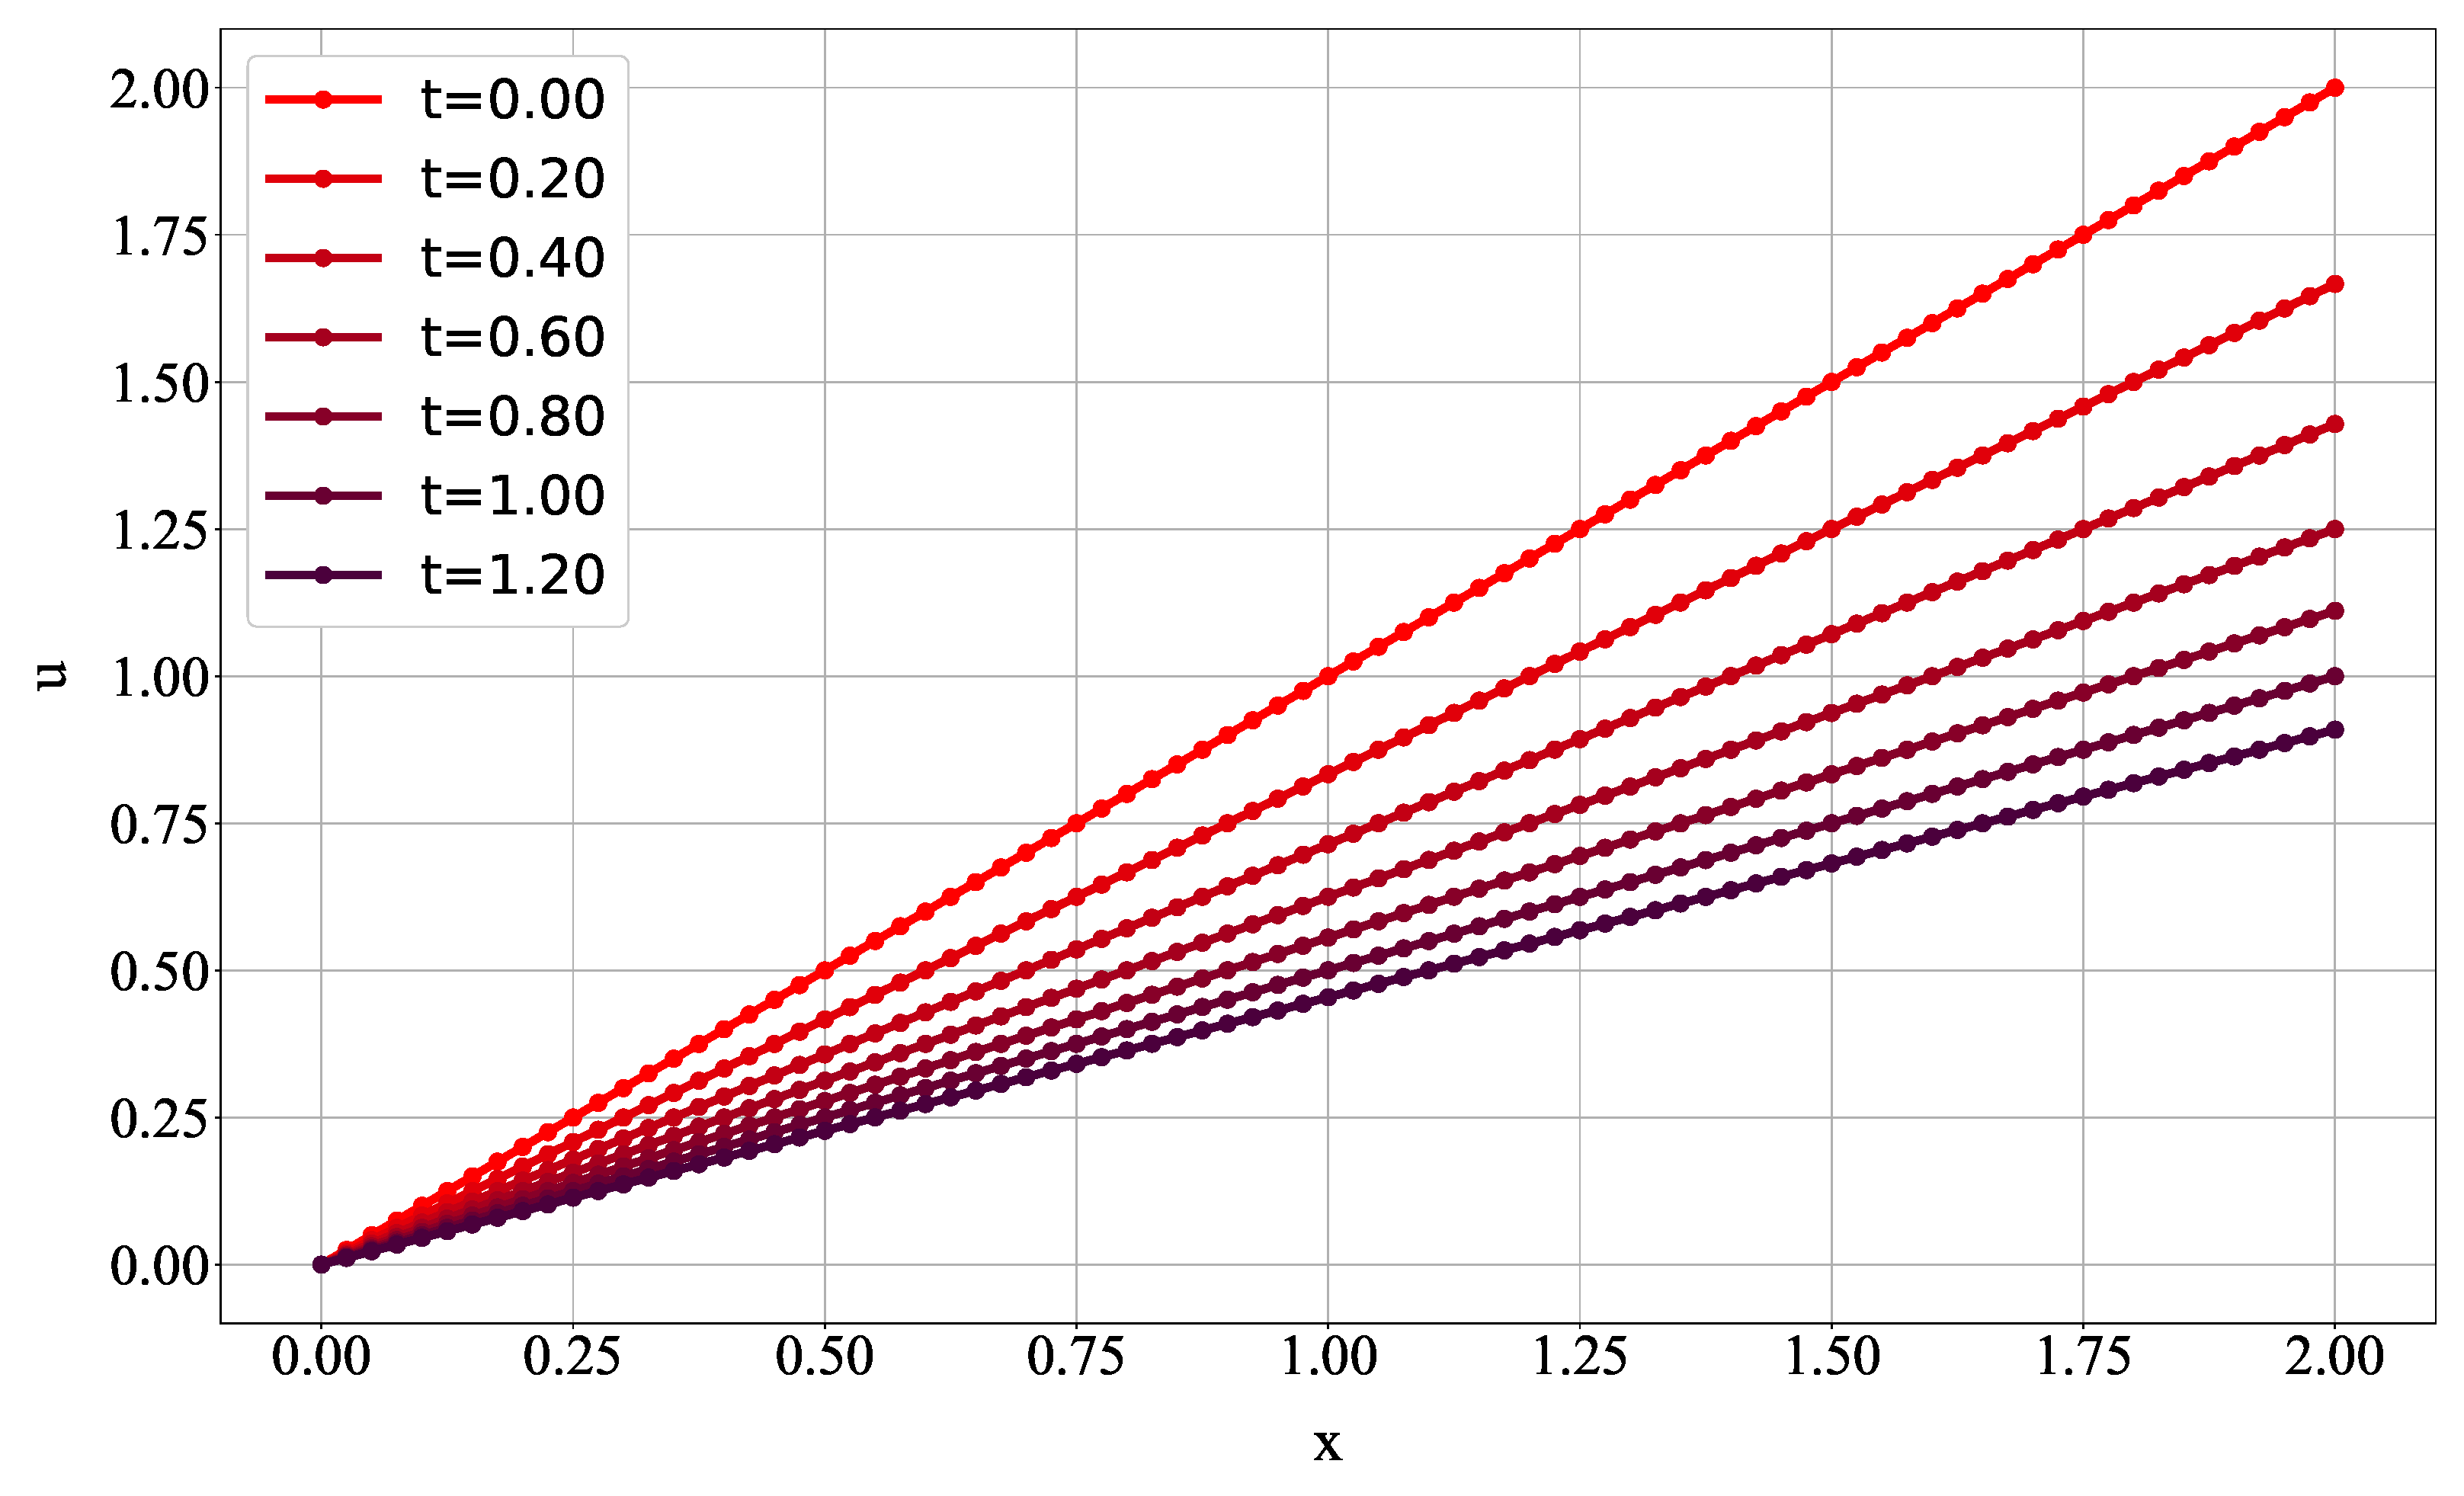
\includegraphics[width=0.425\linewidth]{1.silly.cour05.f2025}}\\
      %\cmidrule{3-4}
      {}                                          & $0.9$    &
        \raisebox{-0.5\totalheight}{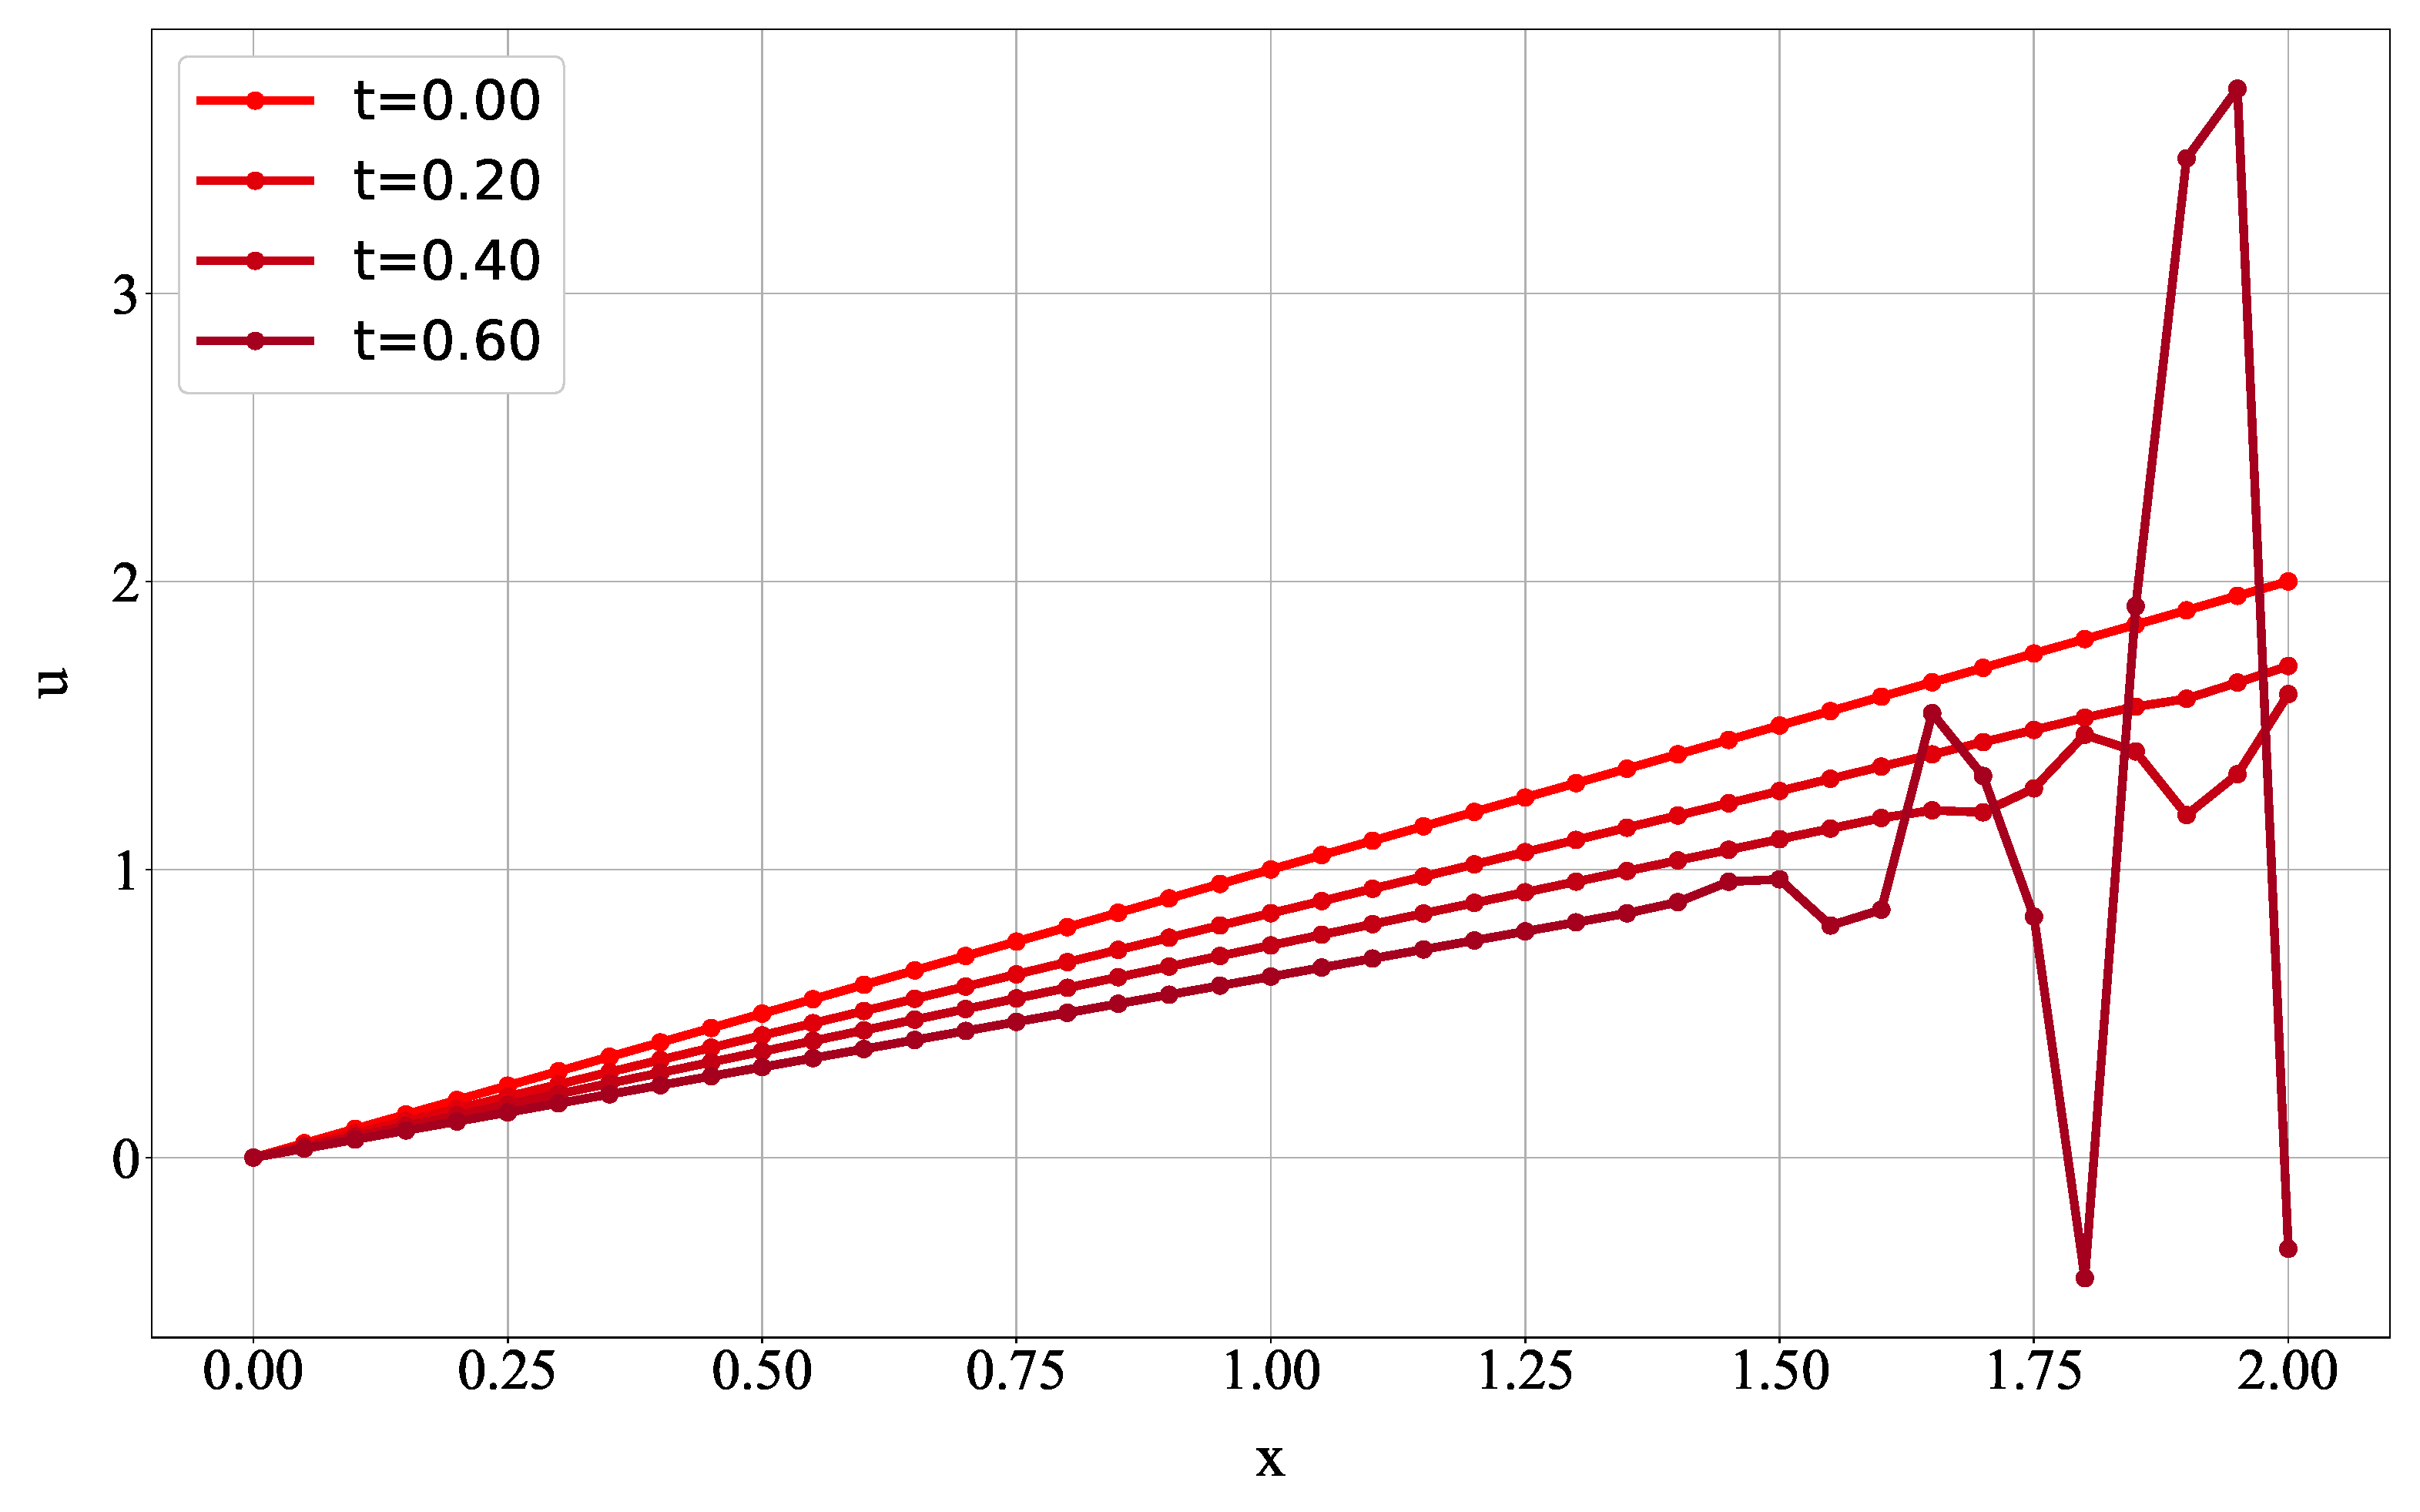
\includegraphics[width=0.425\linewidth]{1.silly.cour09.f2050}} &
        \raisebox{-0.5\totalheight}{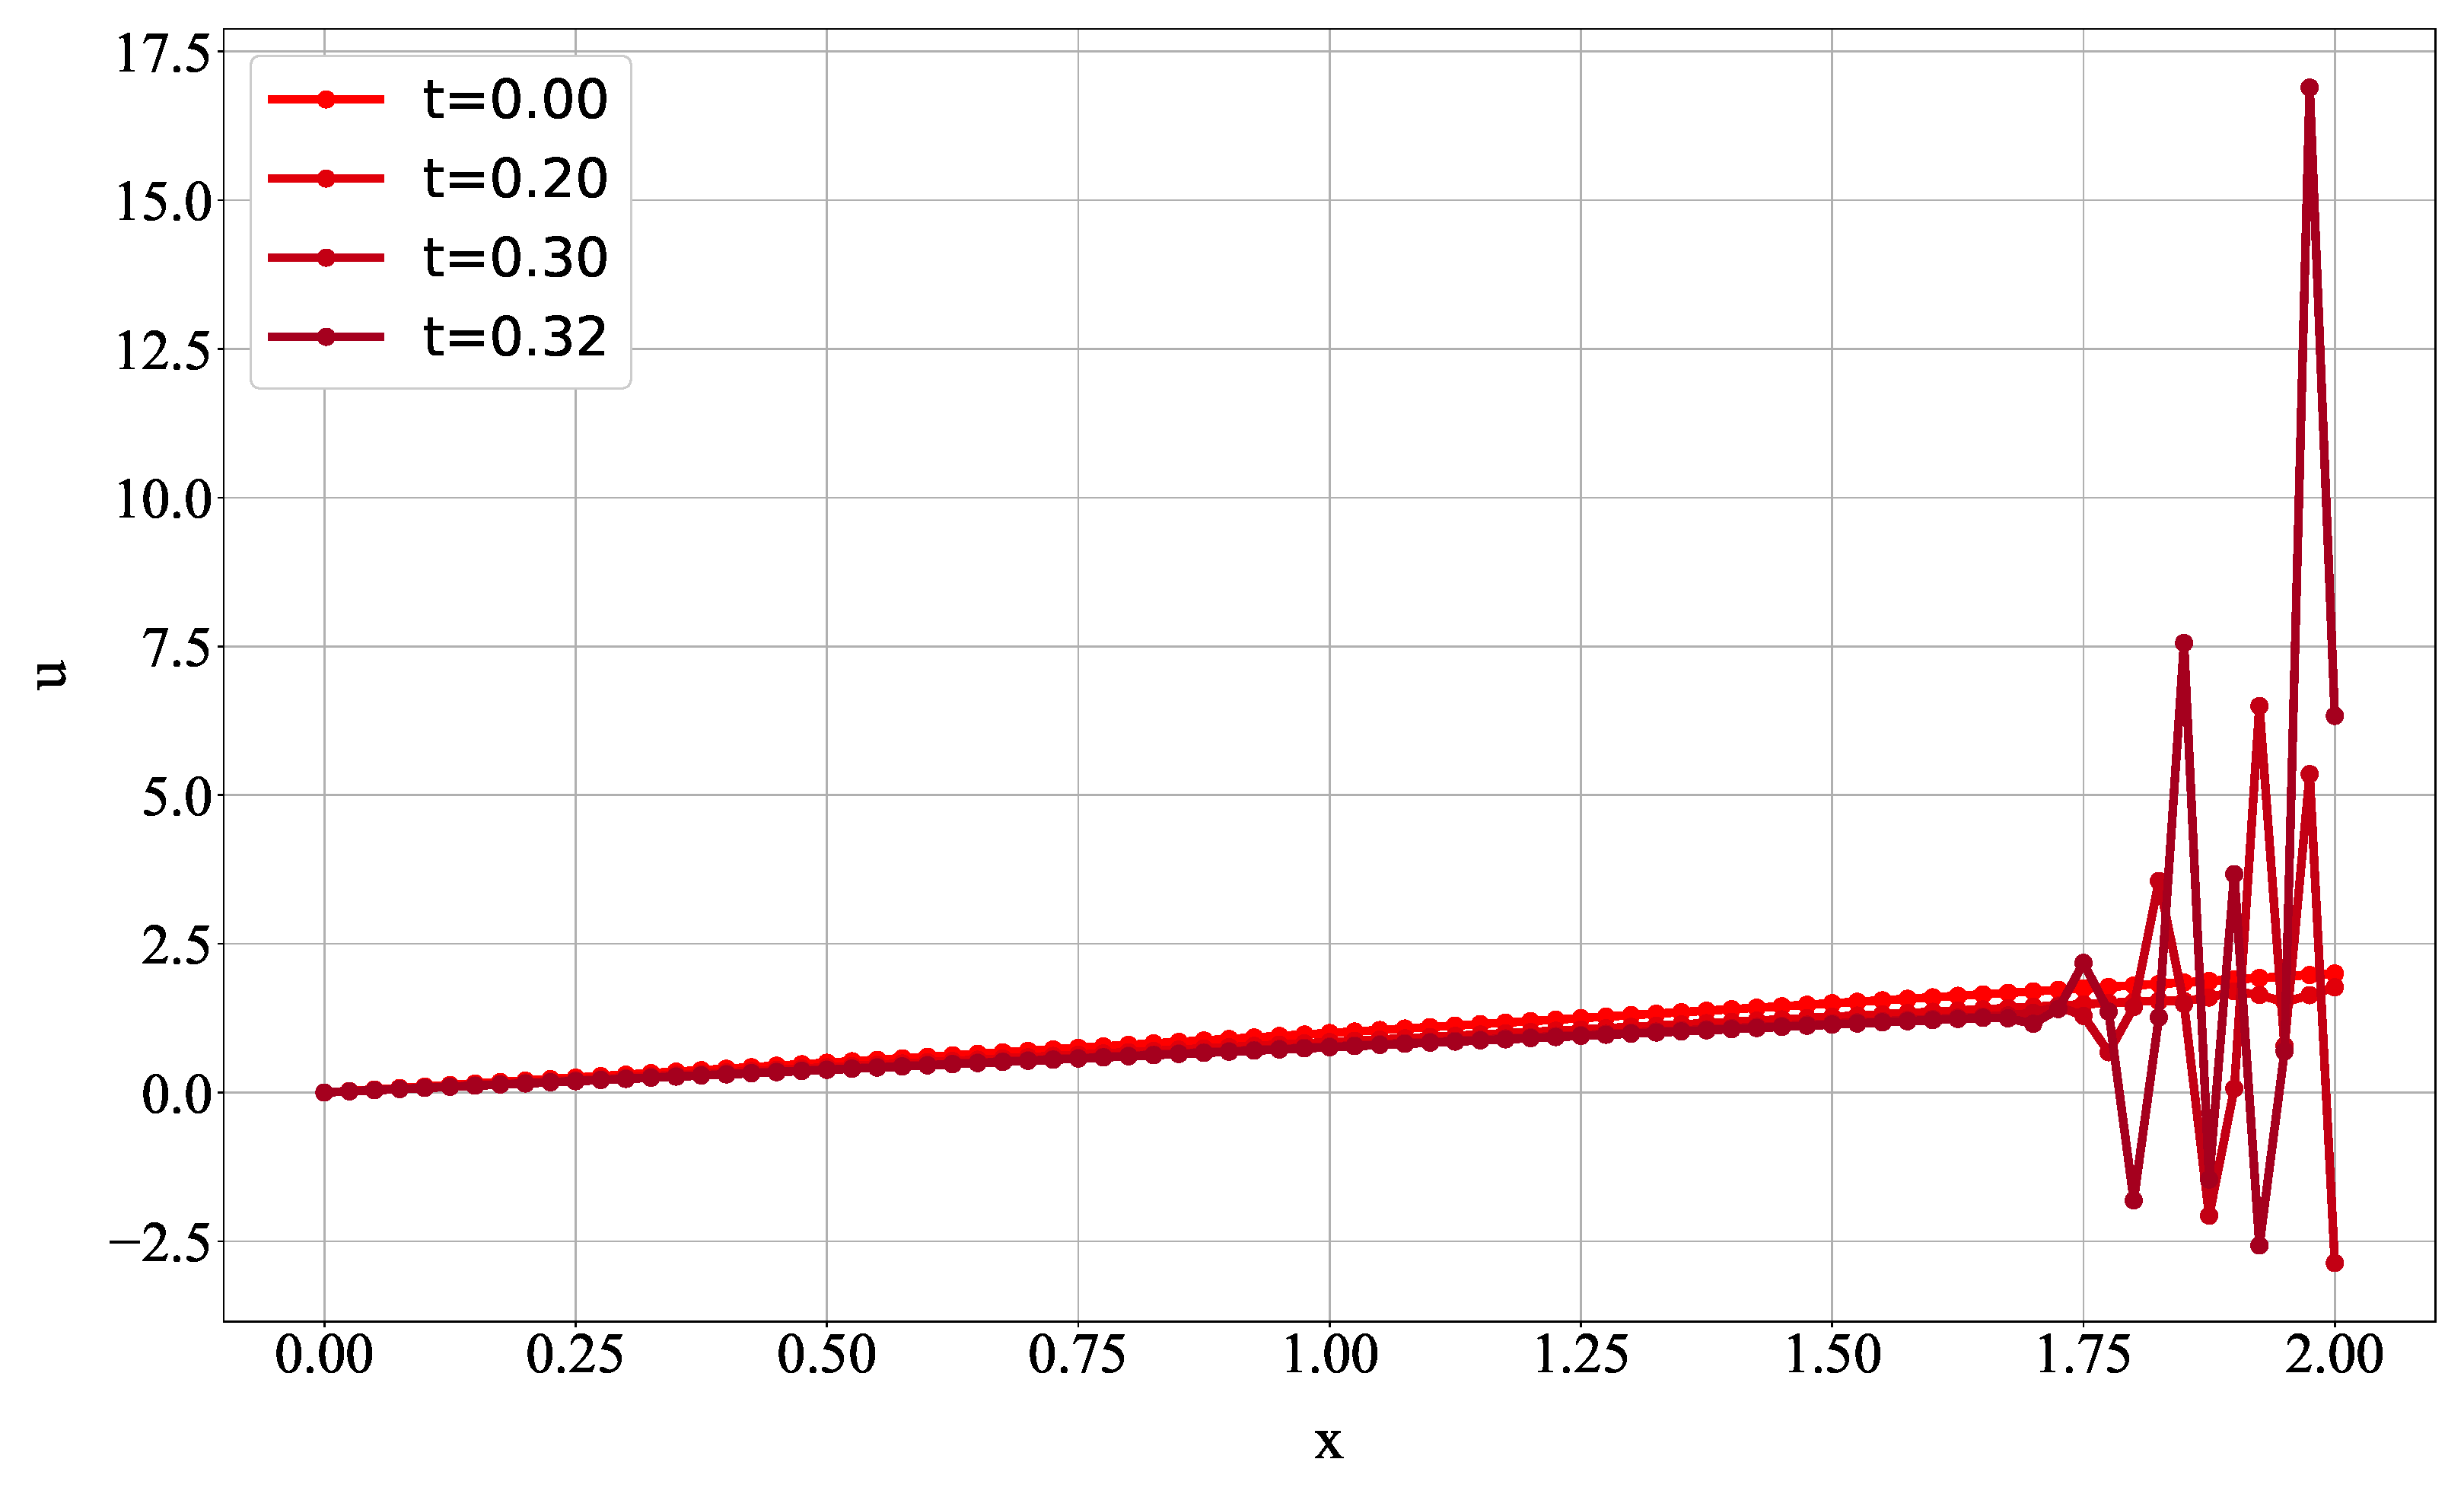
\includegraphics[width=0.425\linewidth]{1.silly.cour09.f2025}}\\
      \bottomrule
    \end{tabular}
  \end{center}
  \end{table}
  
  \begin{table}[p]
  \caption{"`Лакс"' (\ref{sec:lax})}
  \label{plot:lax}
  \begin{center}
    \begin{tabular}{c c c c}
      \toprule
      {$f$}                                       & $\sigma$ & $h_1$ & $h_2$\\
      \midrule
      \multirow{2}{*}{\vspace{\myvspaceOne}$f_1$} & $0.5$    & 
        \raisebox{-0.5\totalheight}{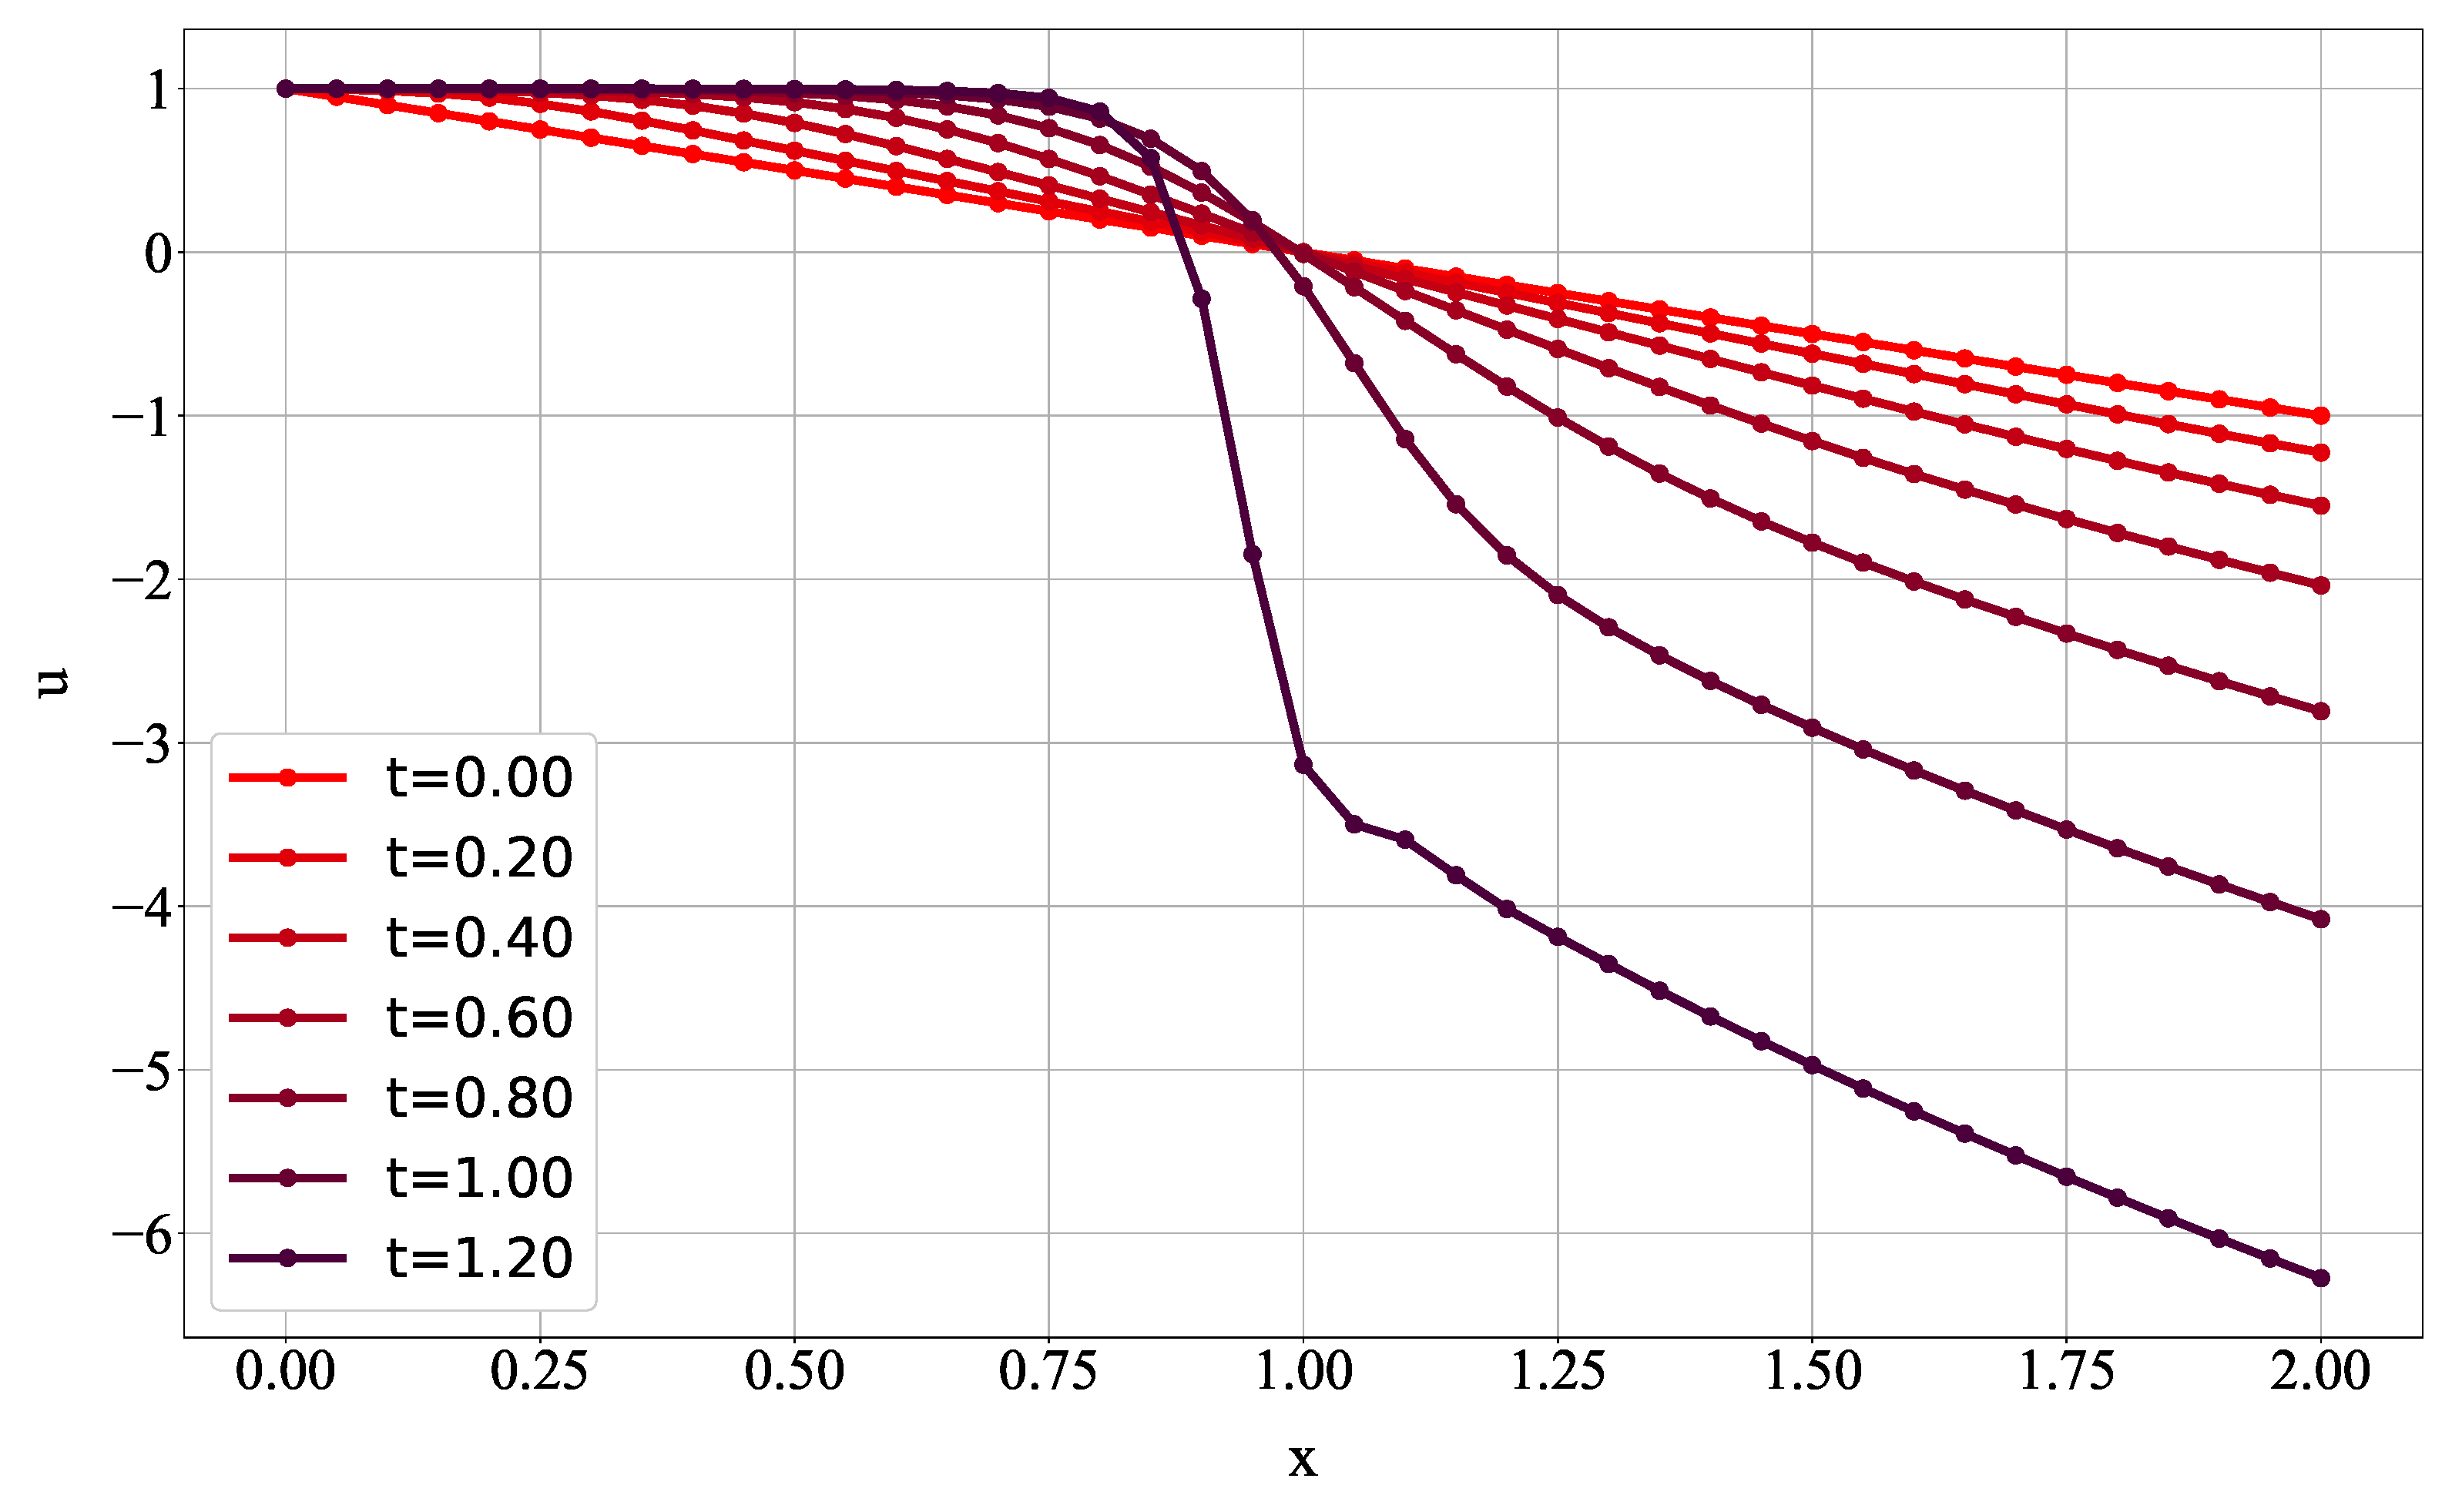
\includegraphics[width=0.425\linewidth]{2.lax.cour05.f1050}} &
        \raisebox{-0.5\totalheight}{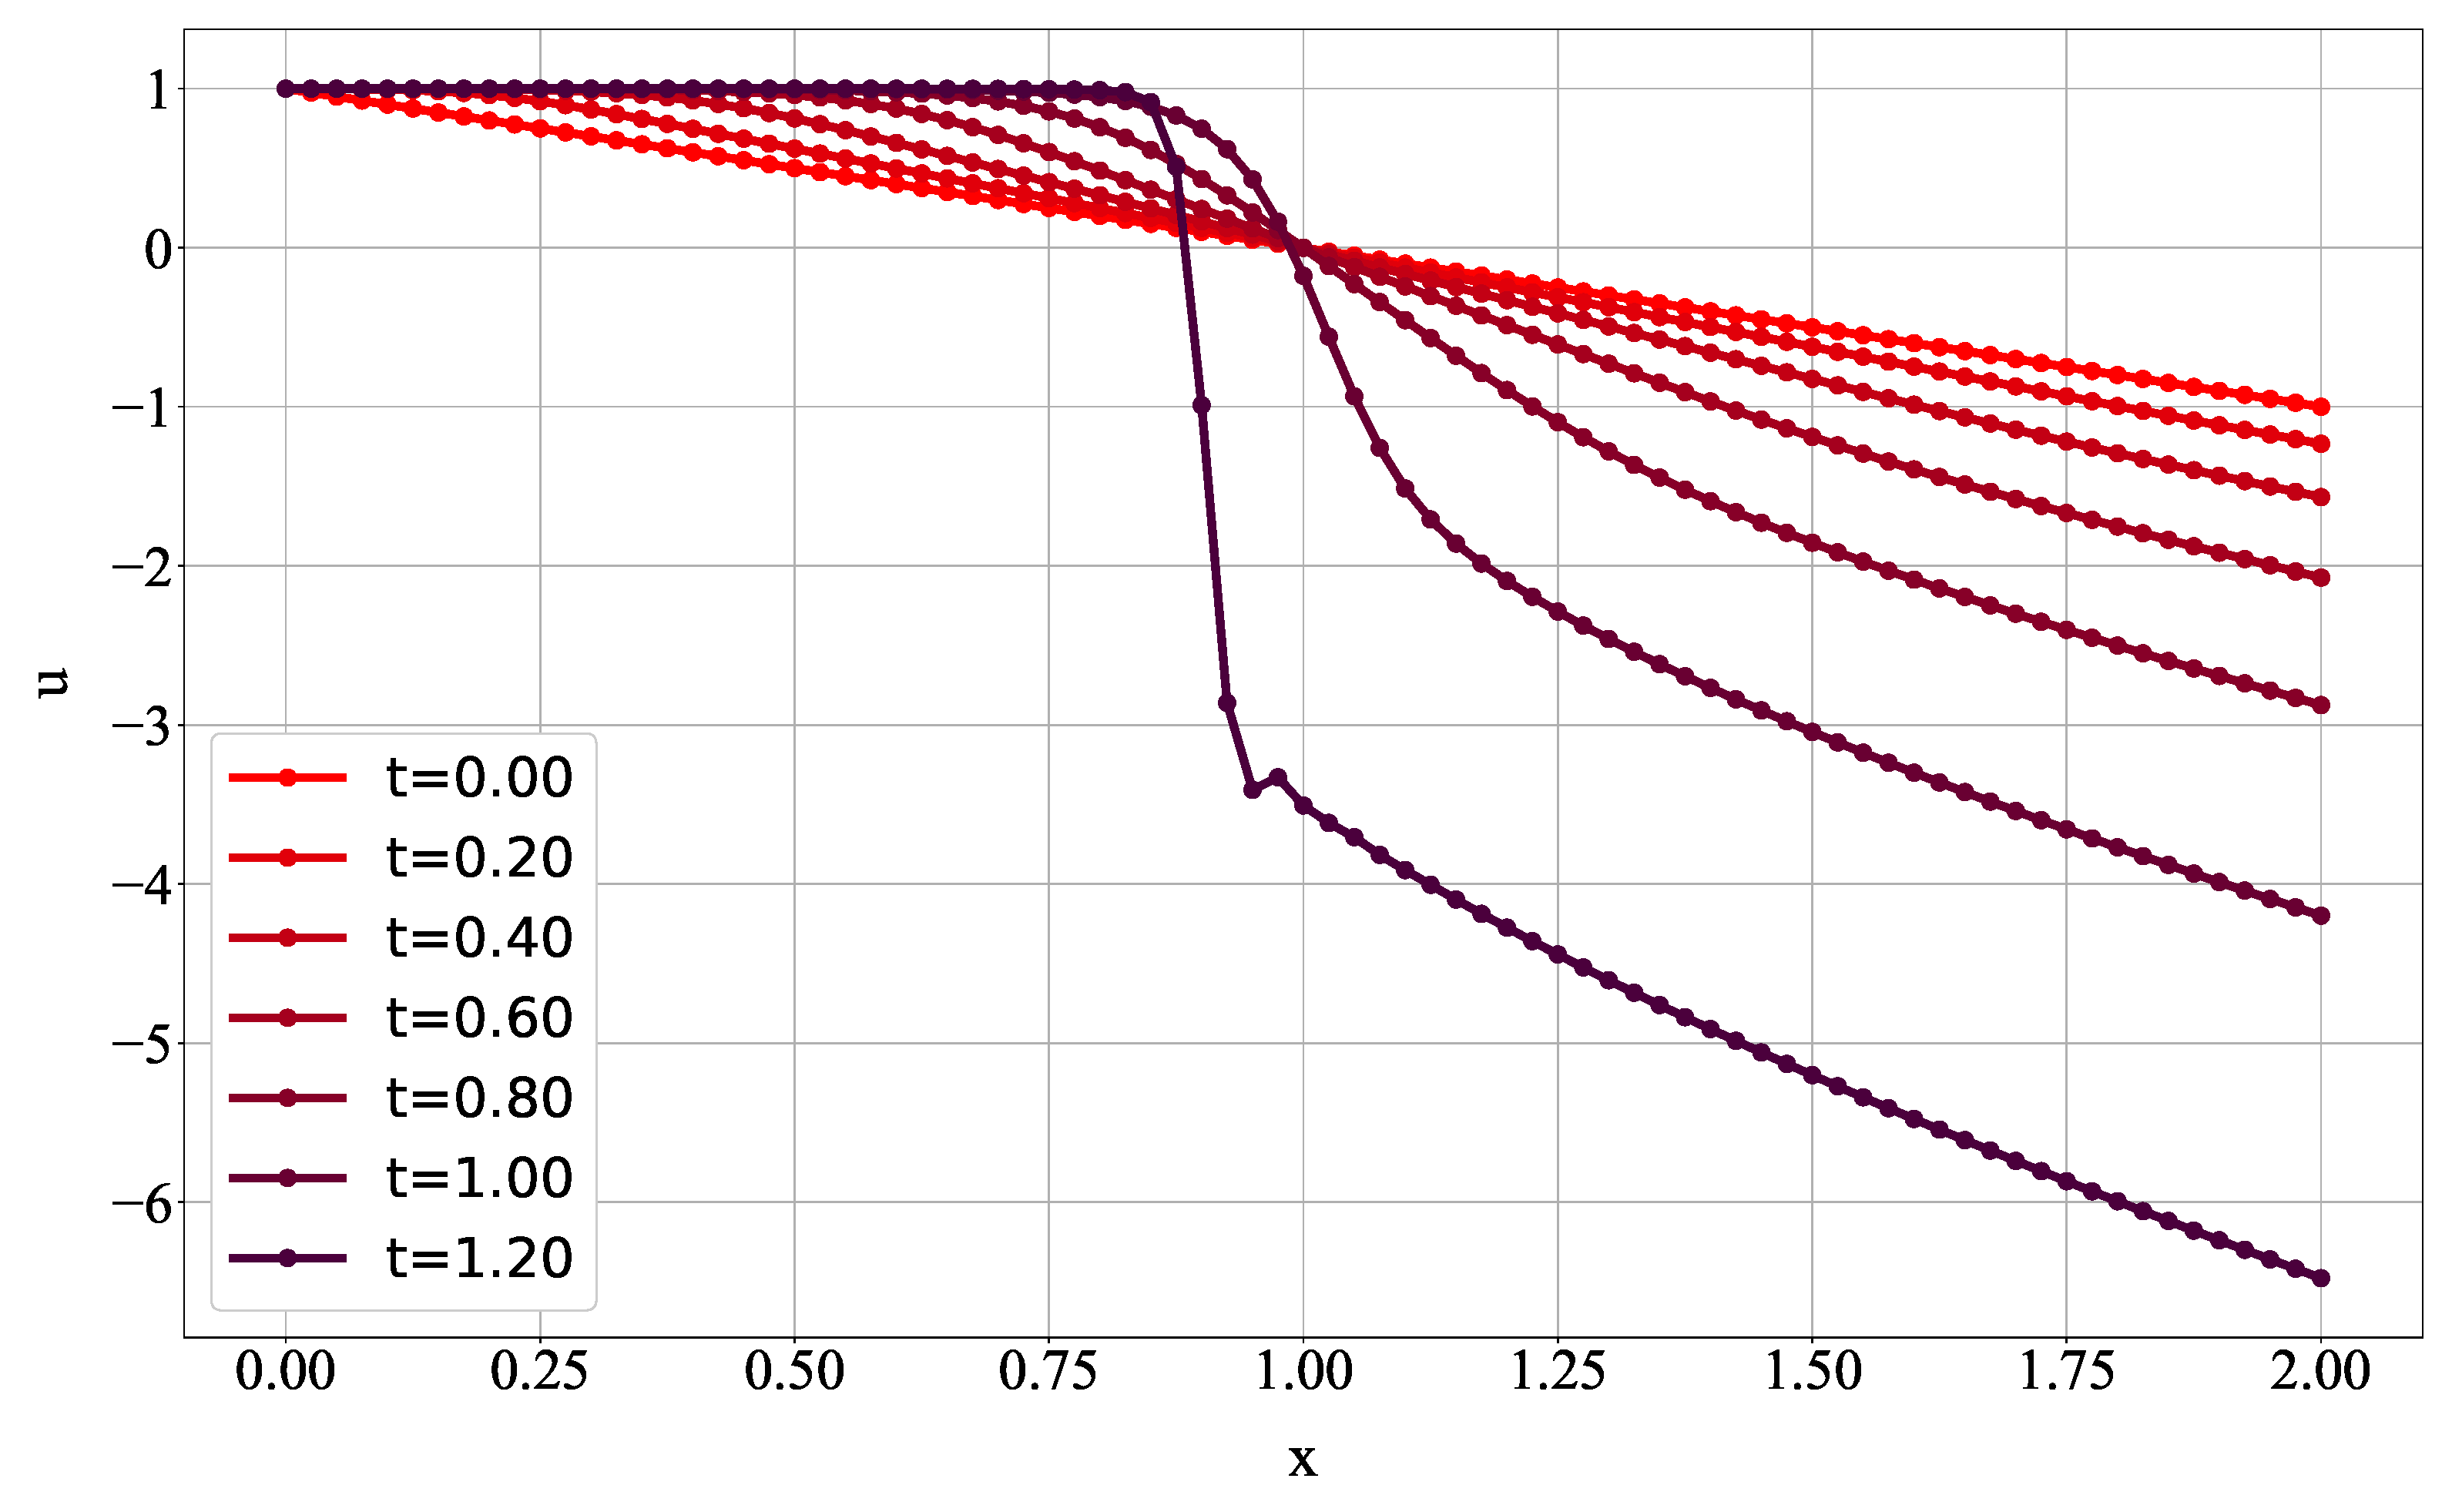
\includegraphics[width=0.425\linewidth]{2.lax.cour05.f1025}}\\
      %\cmidrule{3-4}
      {}                                          & $0.9$    &
        \raisebox{-0.5\totalheight}{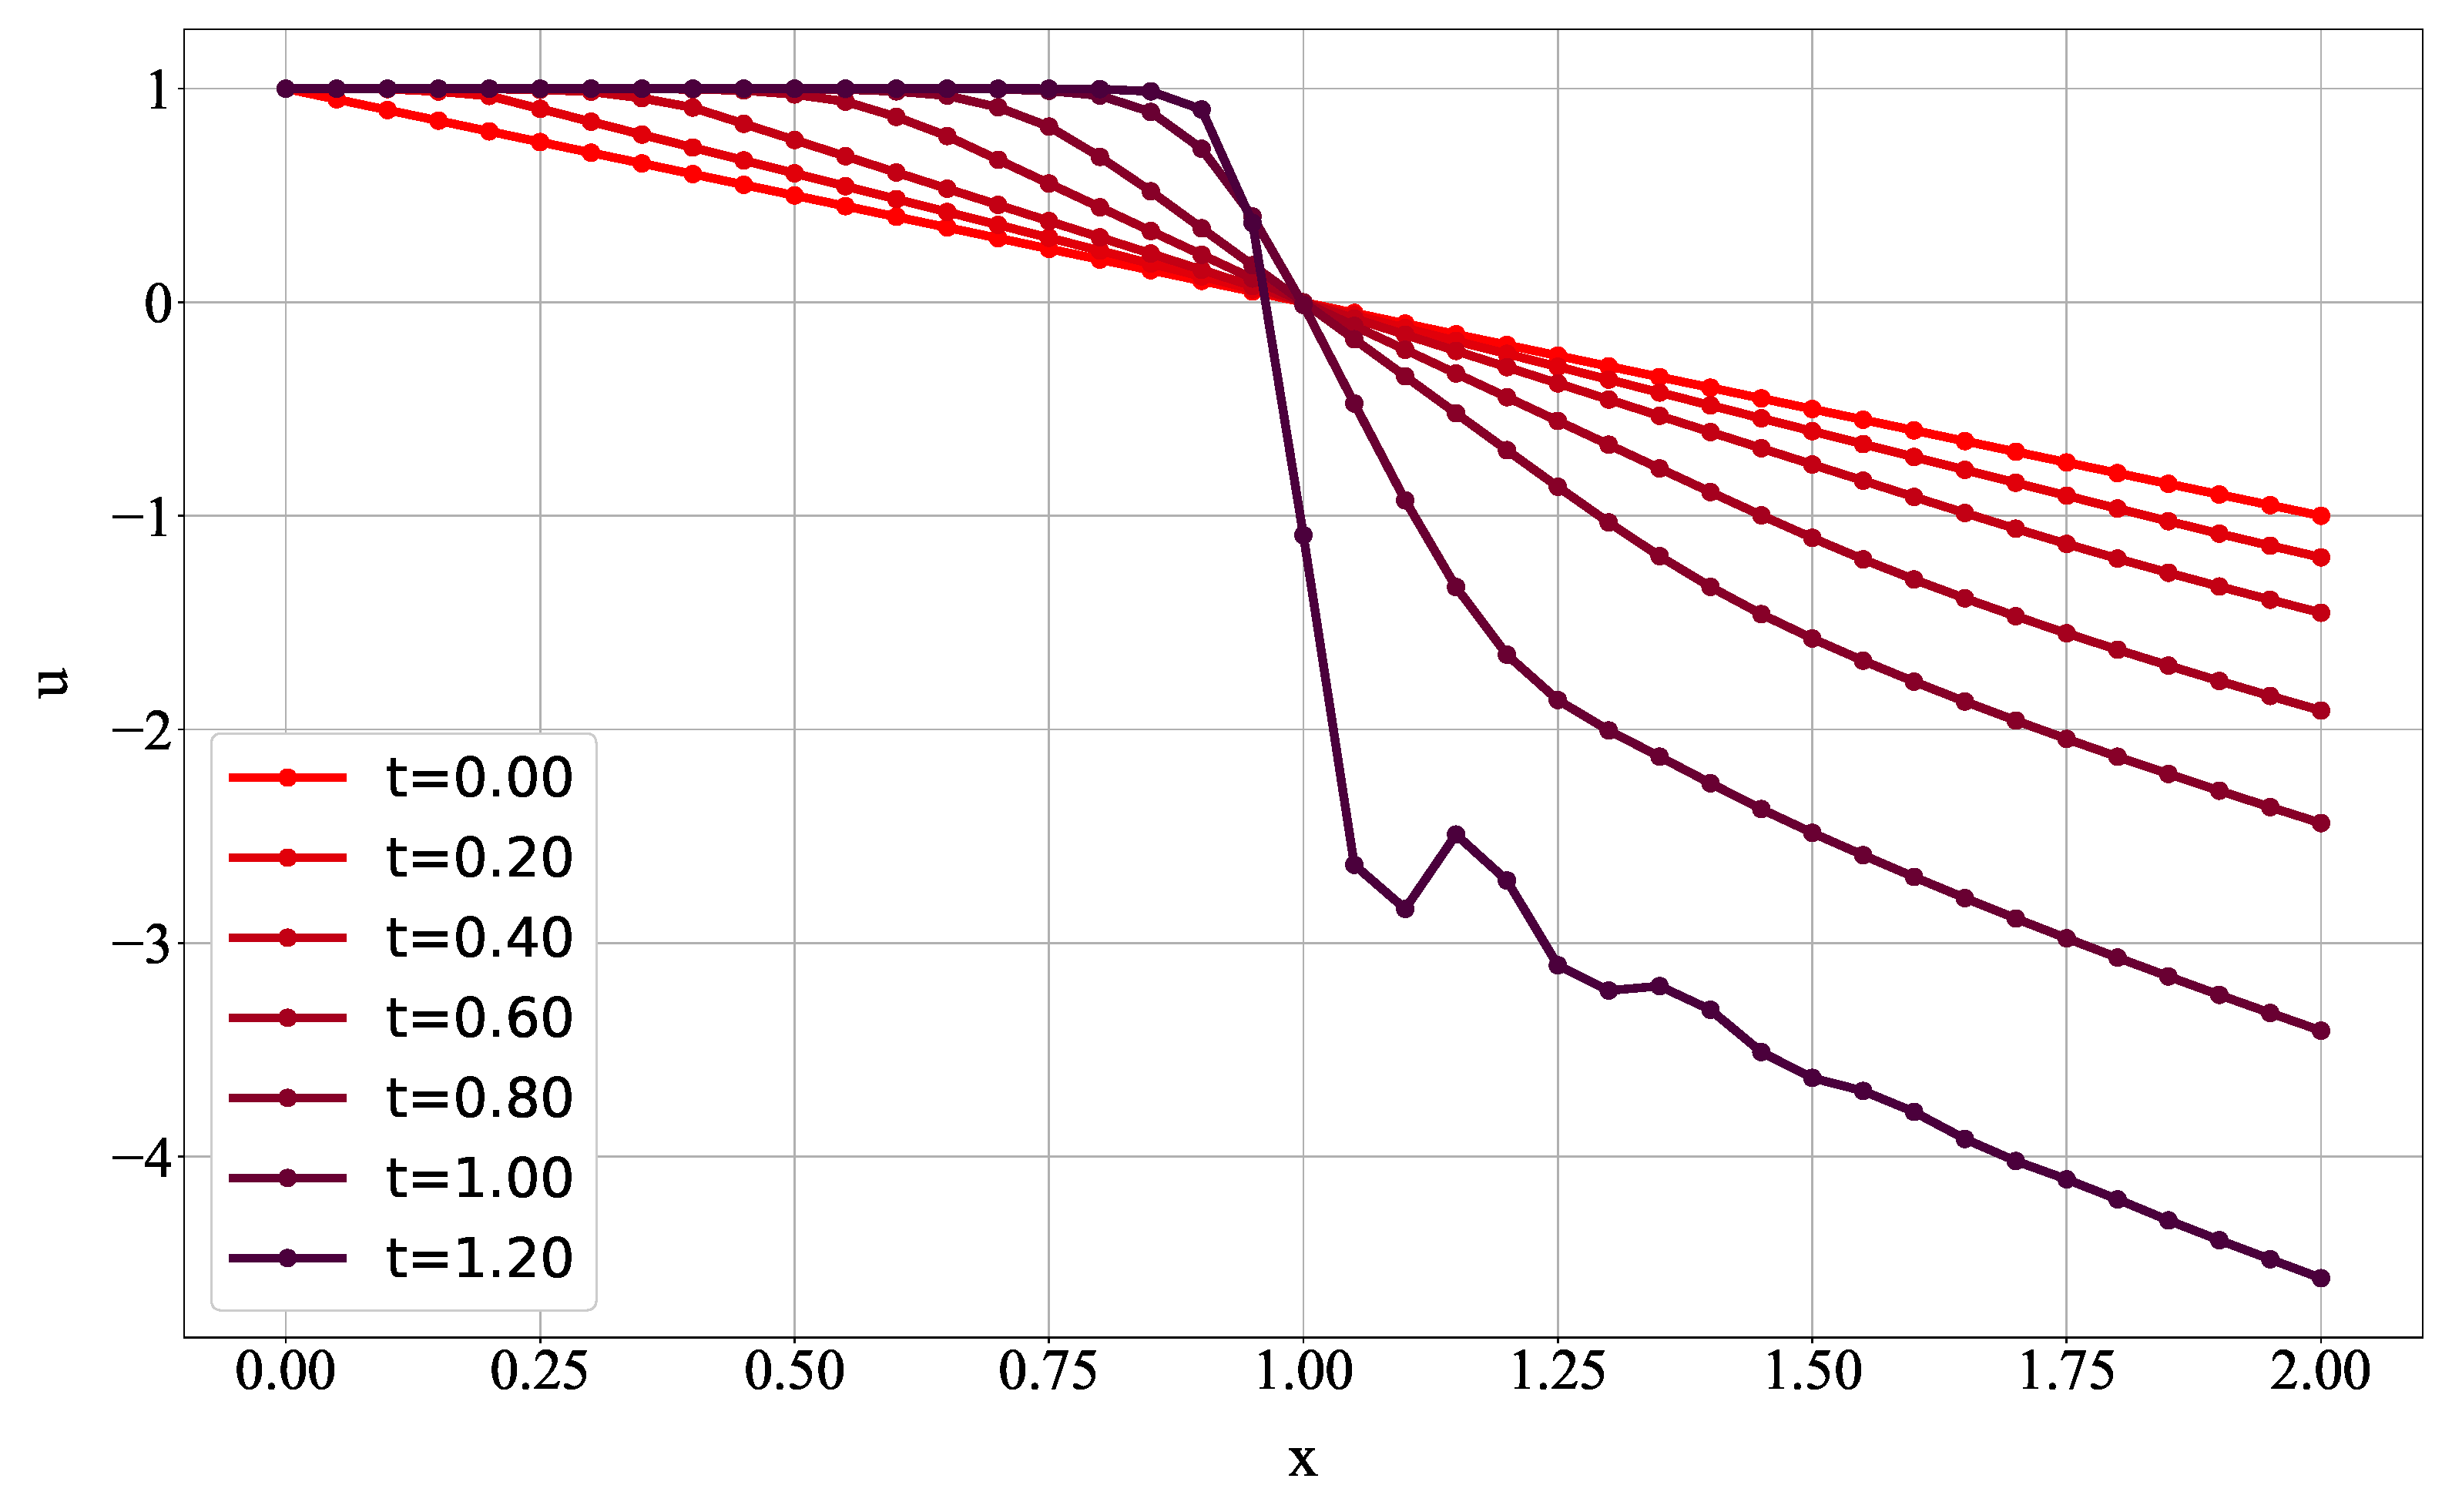
\includegraphics[width=0.425\linewidth]{2.lax.cour09.f1050}} & 
        \raisebox{-0.5\totalheight}{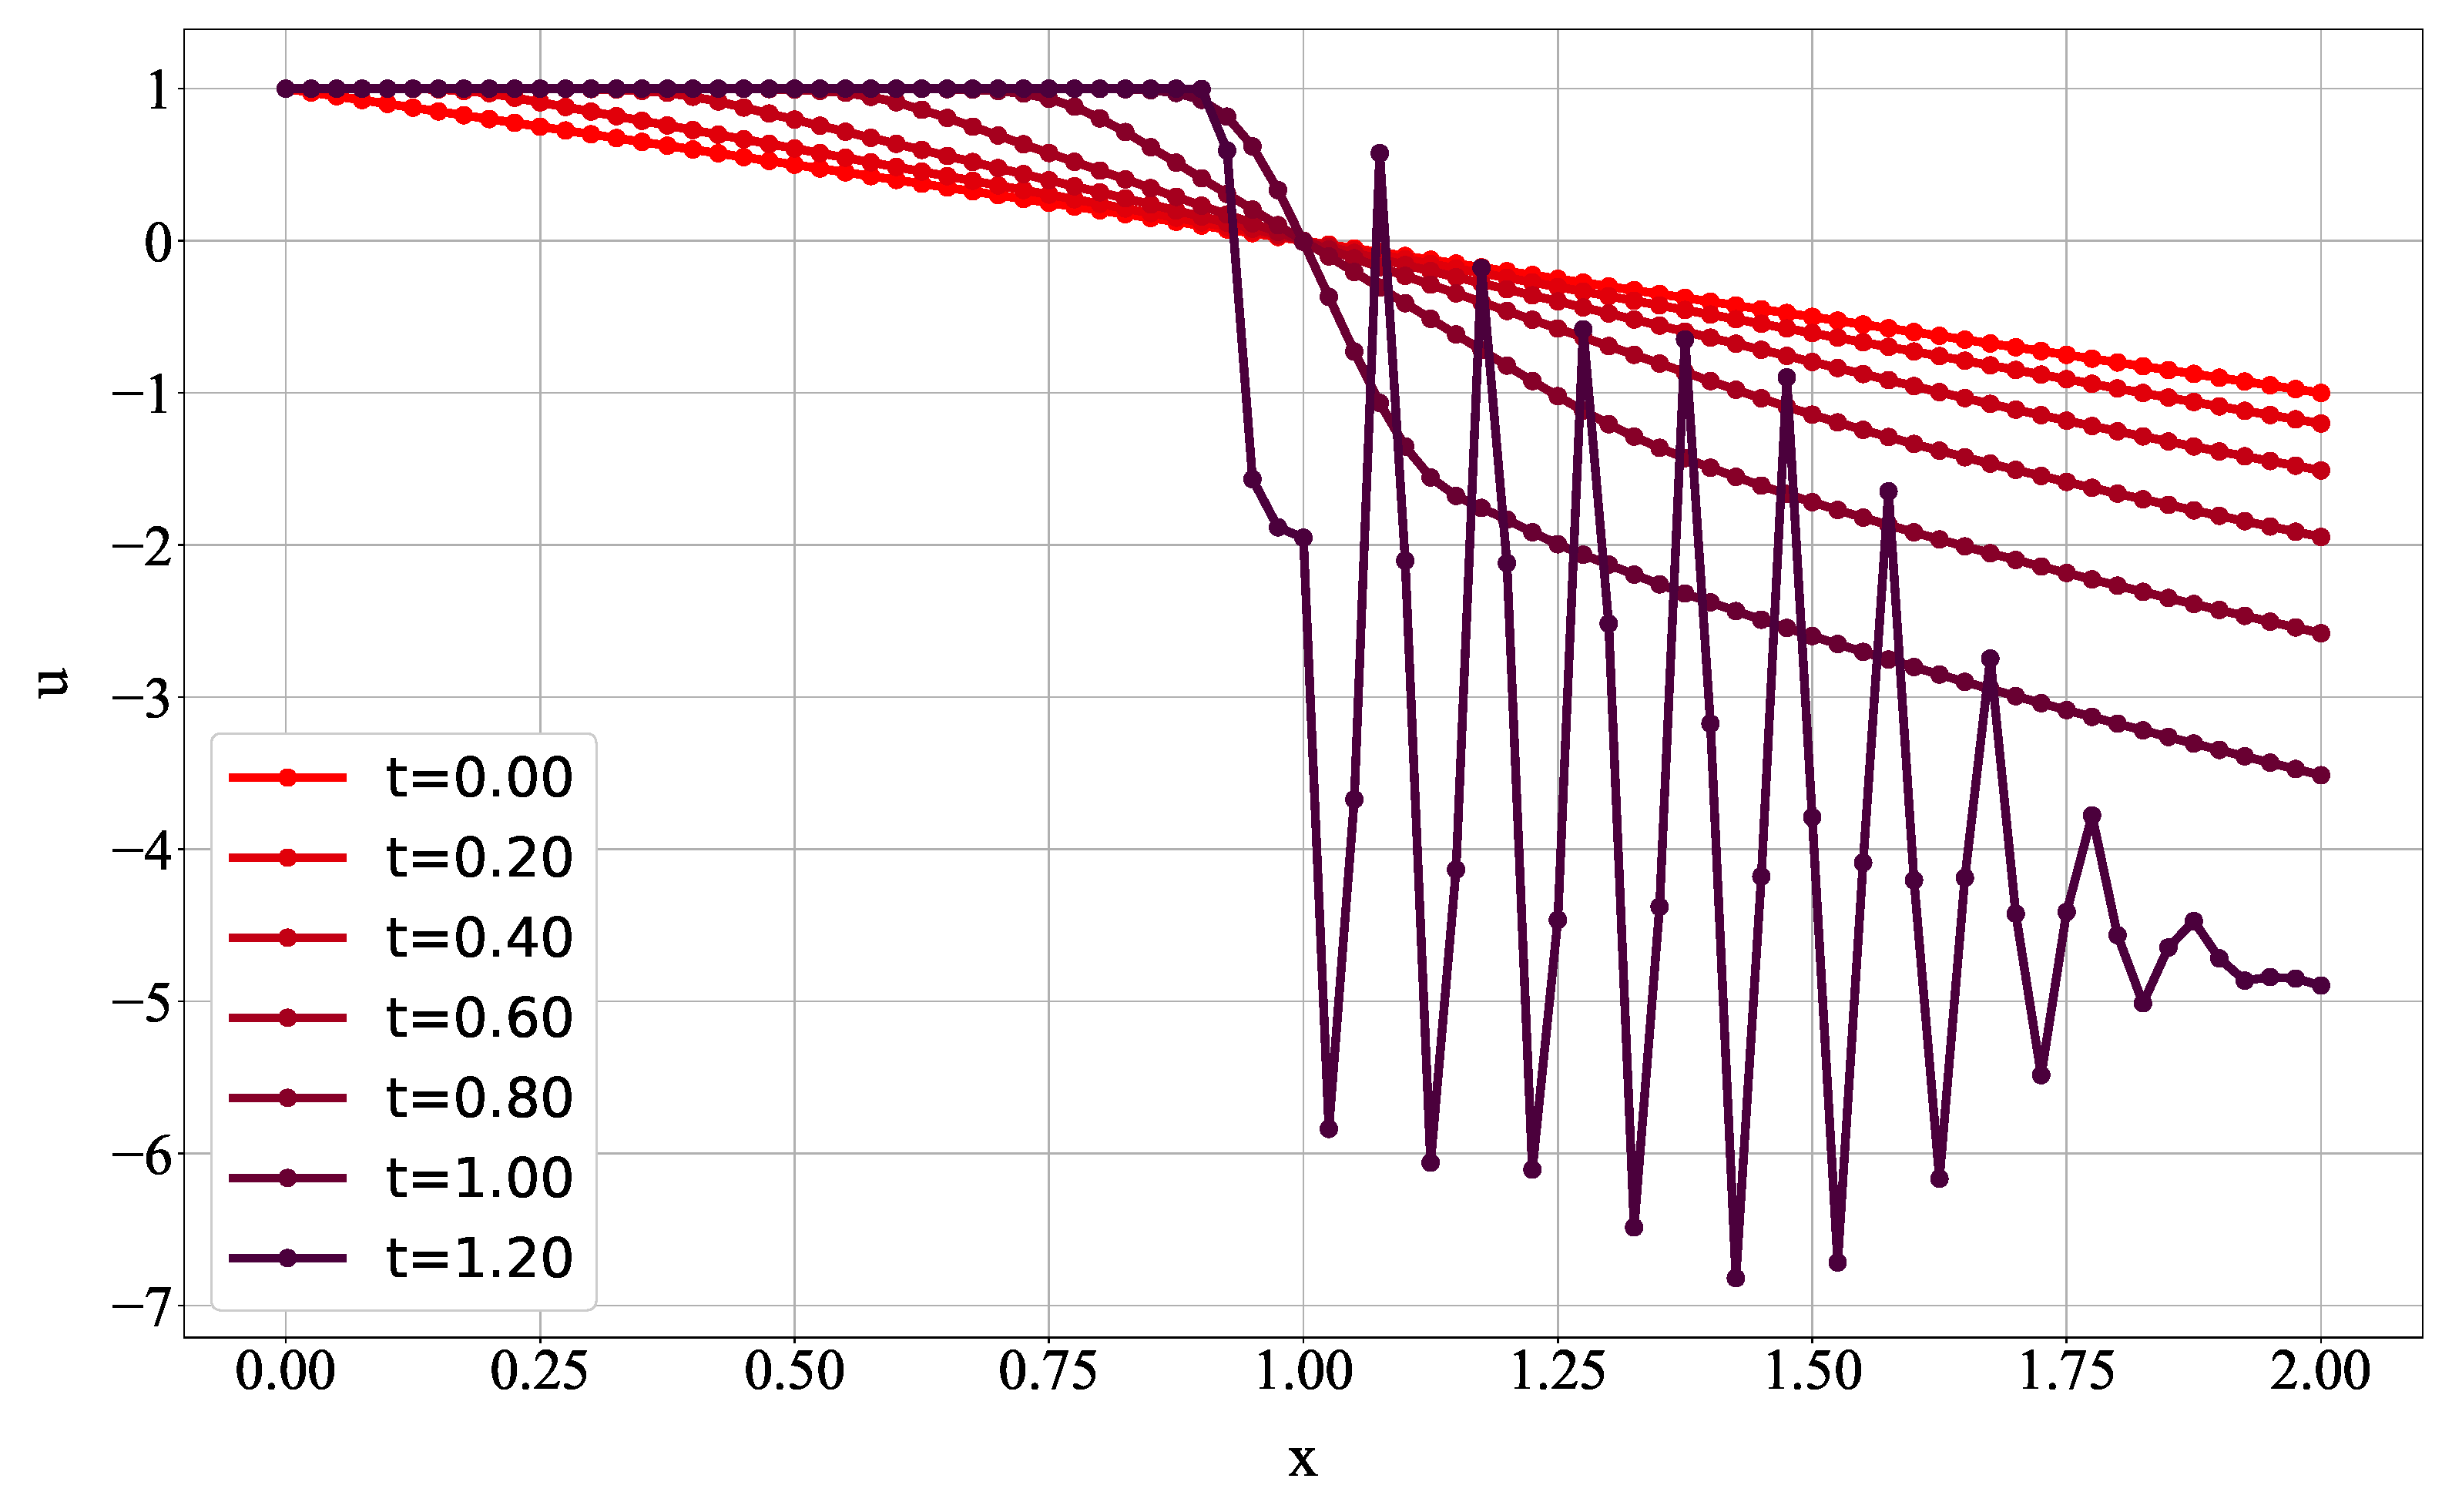
\includegraphics[width=0.425\linewidth]{2.lax.cour09.f1025}}\\
      \midrule
      \multirow{2}{*}{\vspace{\myvspaceOne}$f_2$} & $0.5$    &
        \raisebox{-0.5\totalheight}{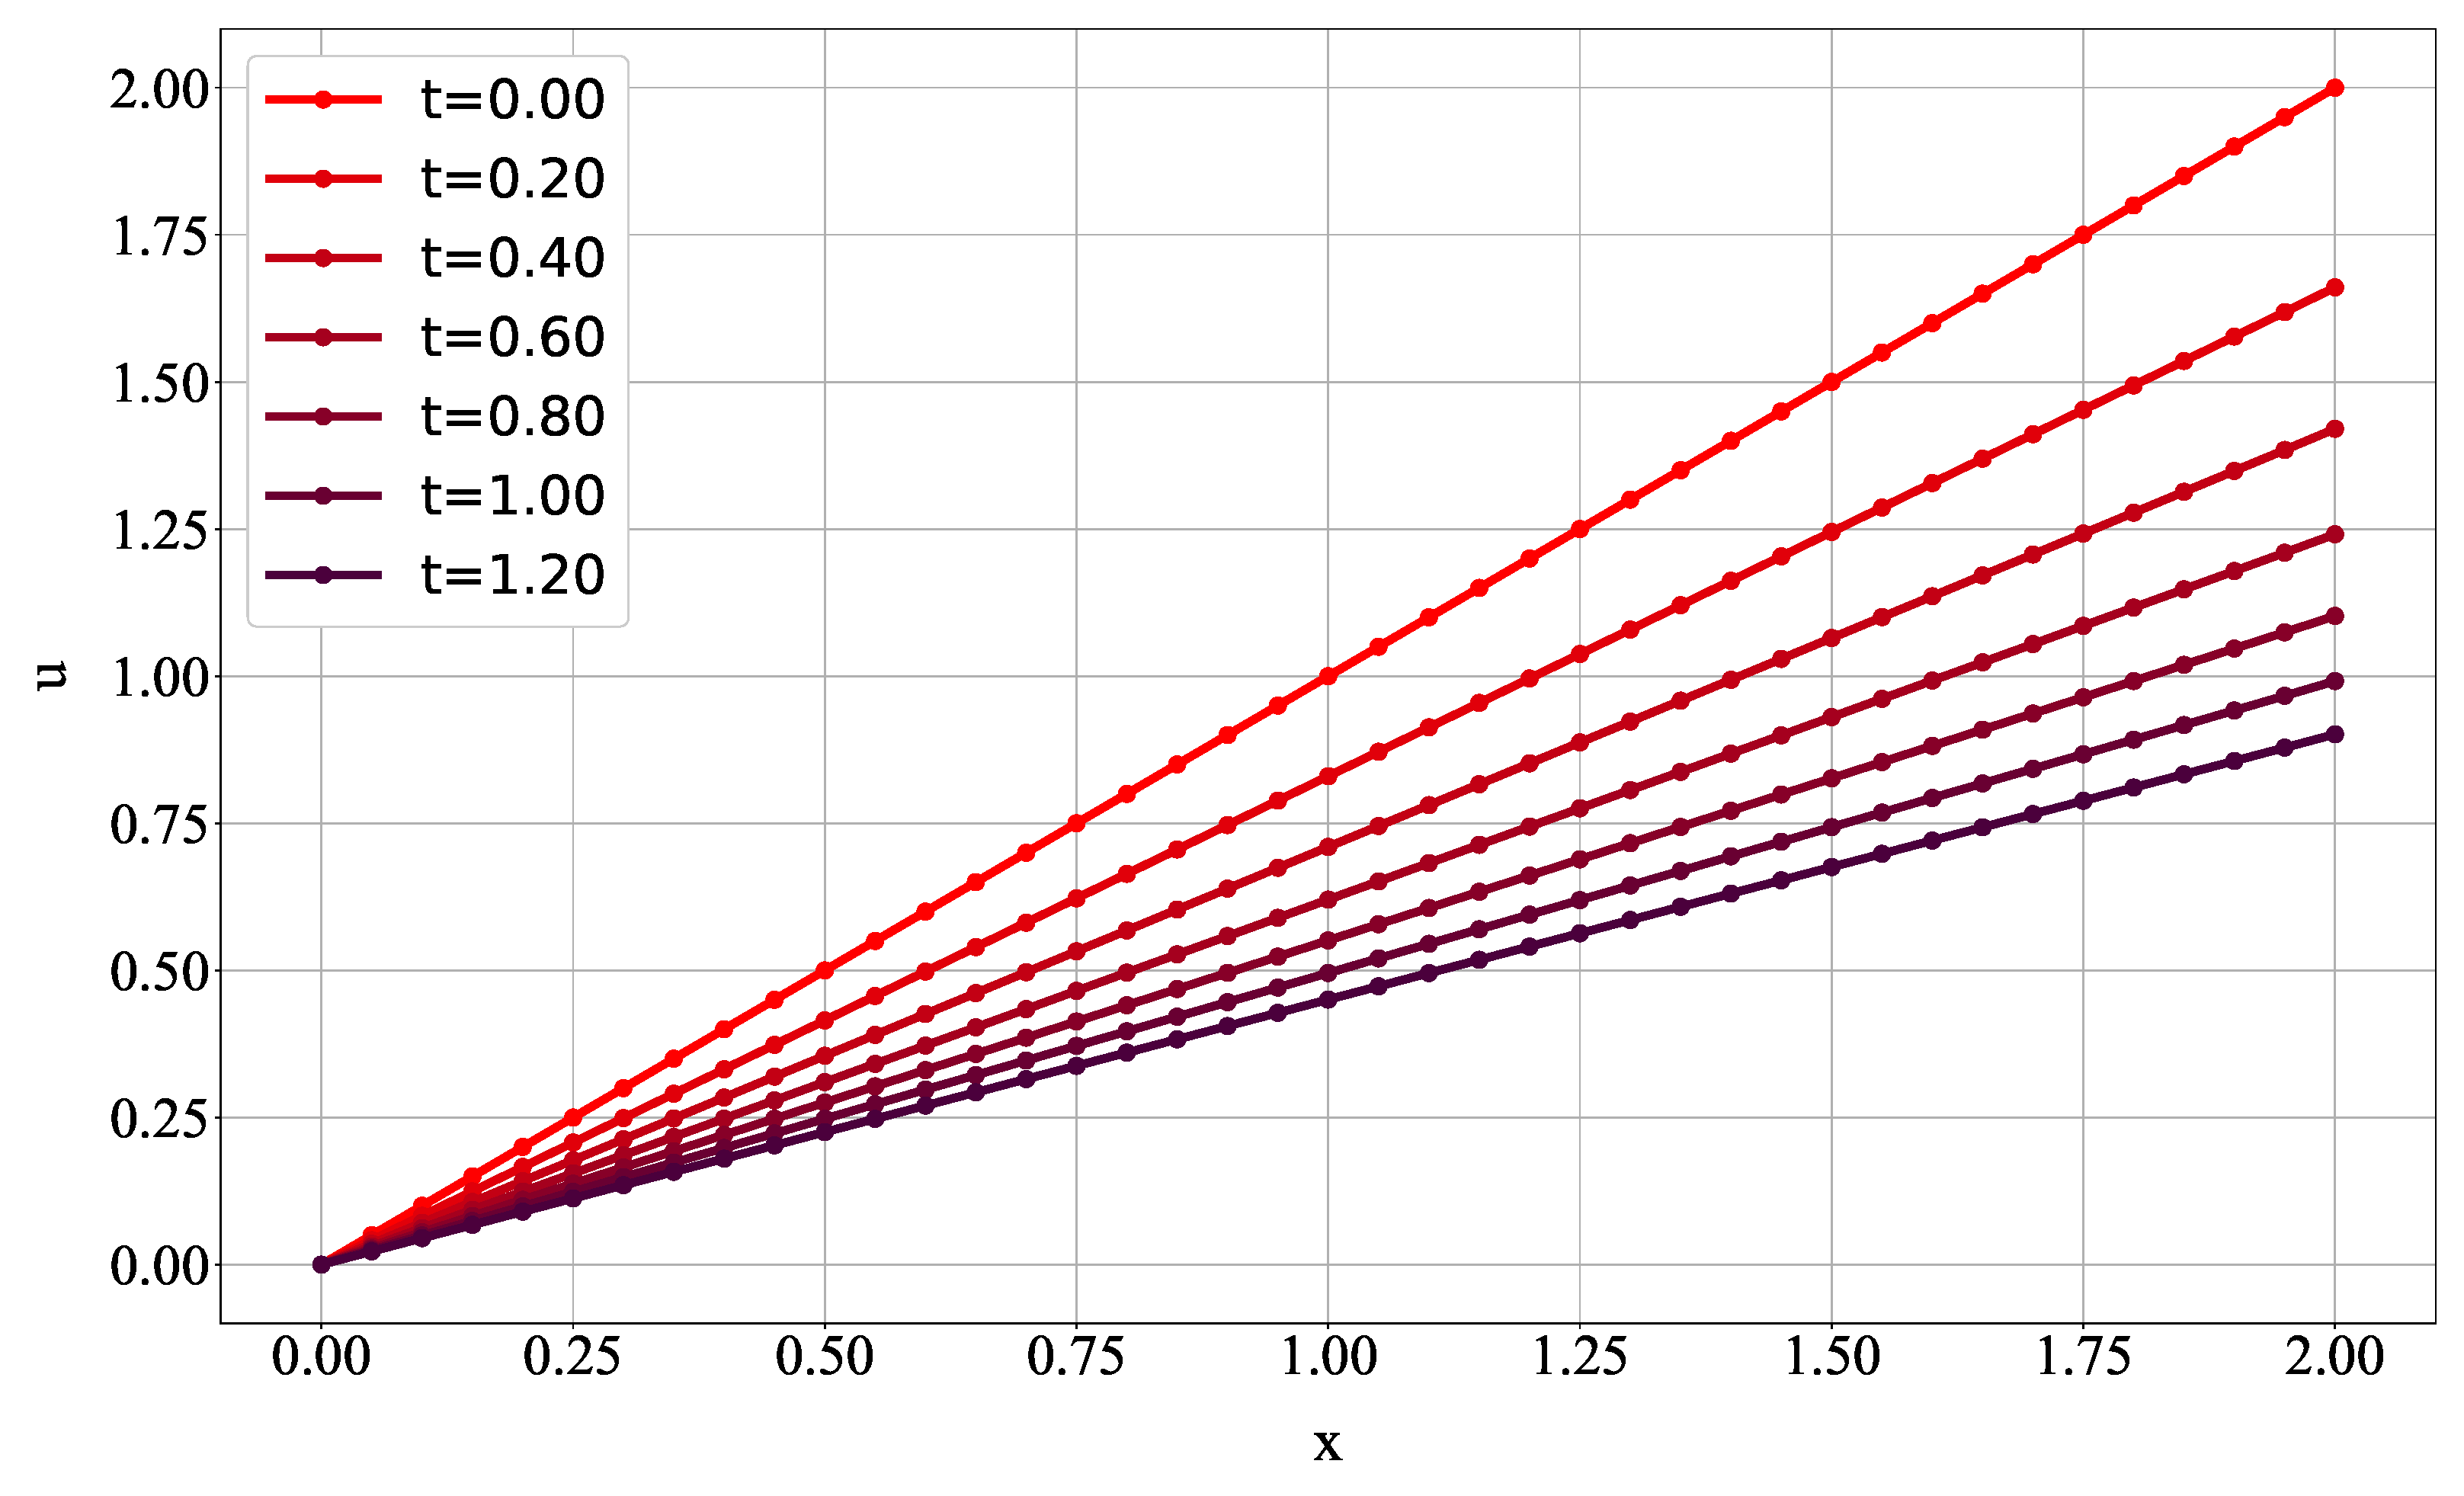
\includegraphics[width=0.425\linewidth]{2.lax.cour05.f2050}} &
        \raisebox{-0.5\totalheight}{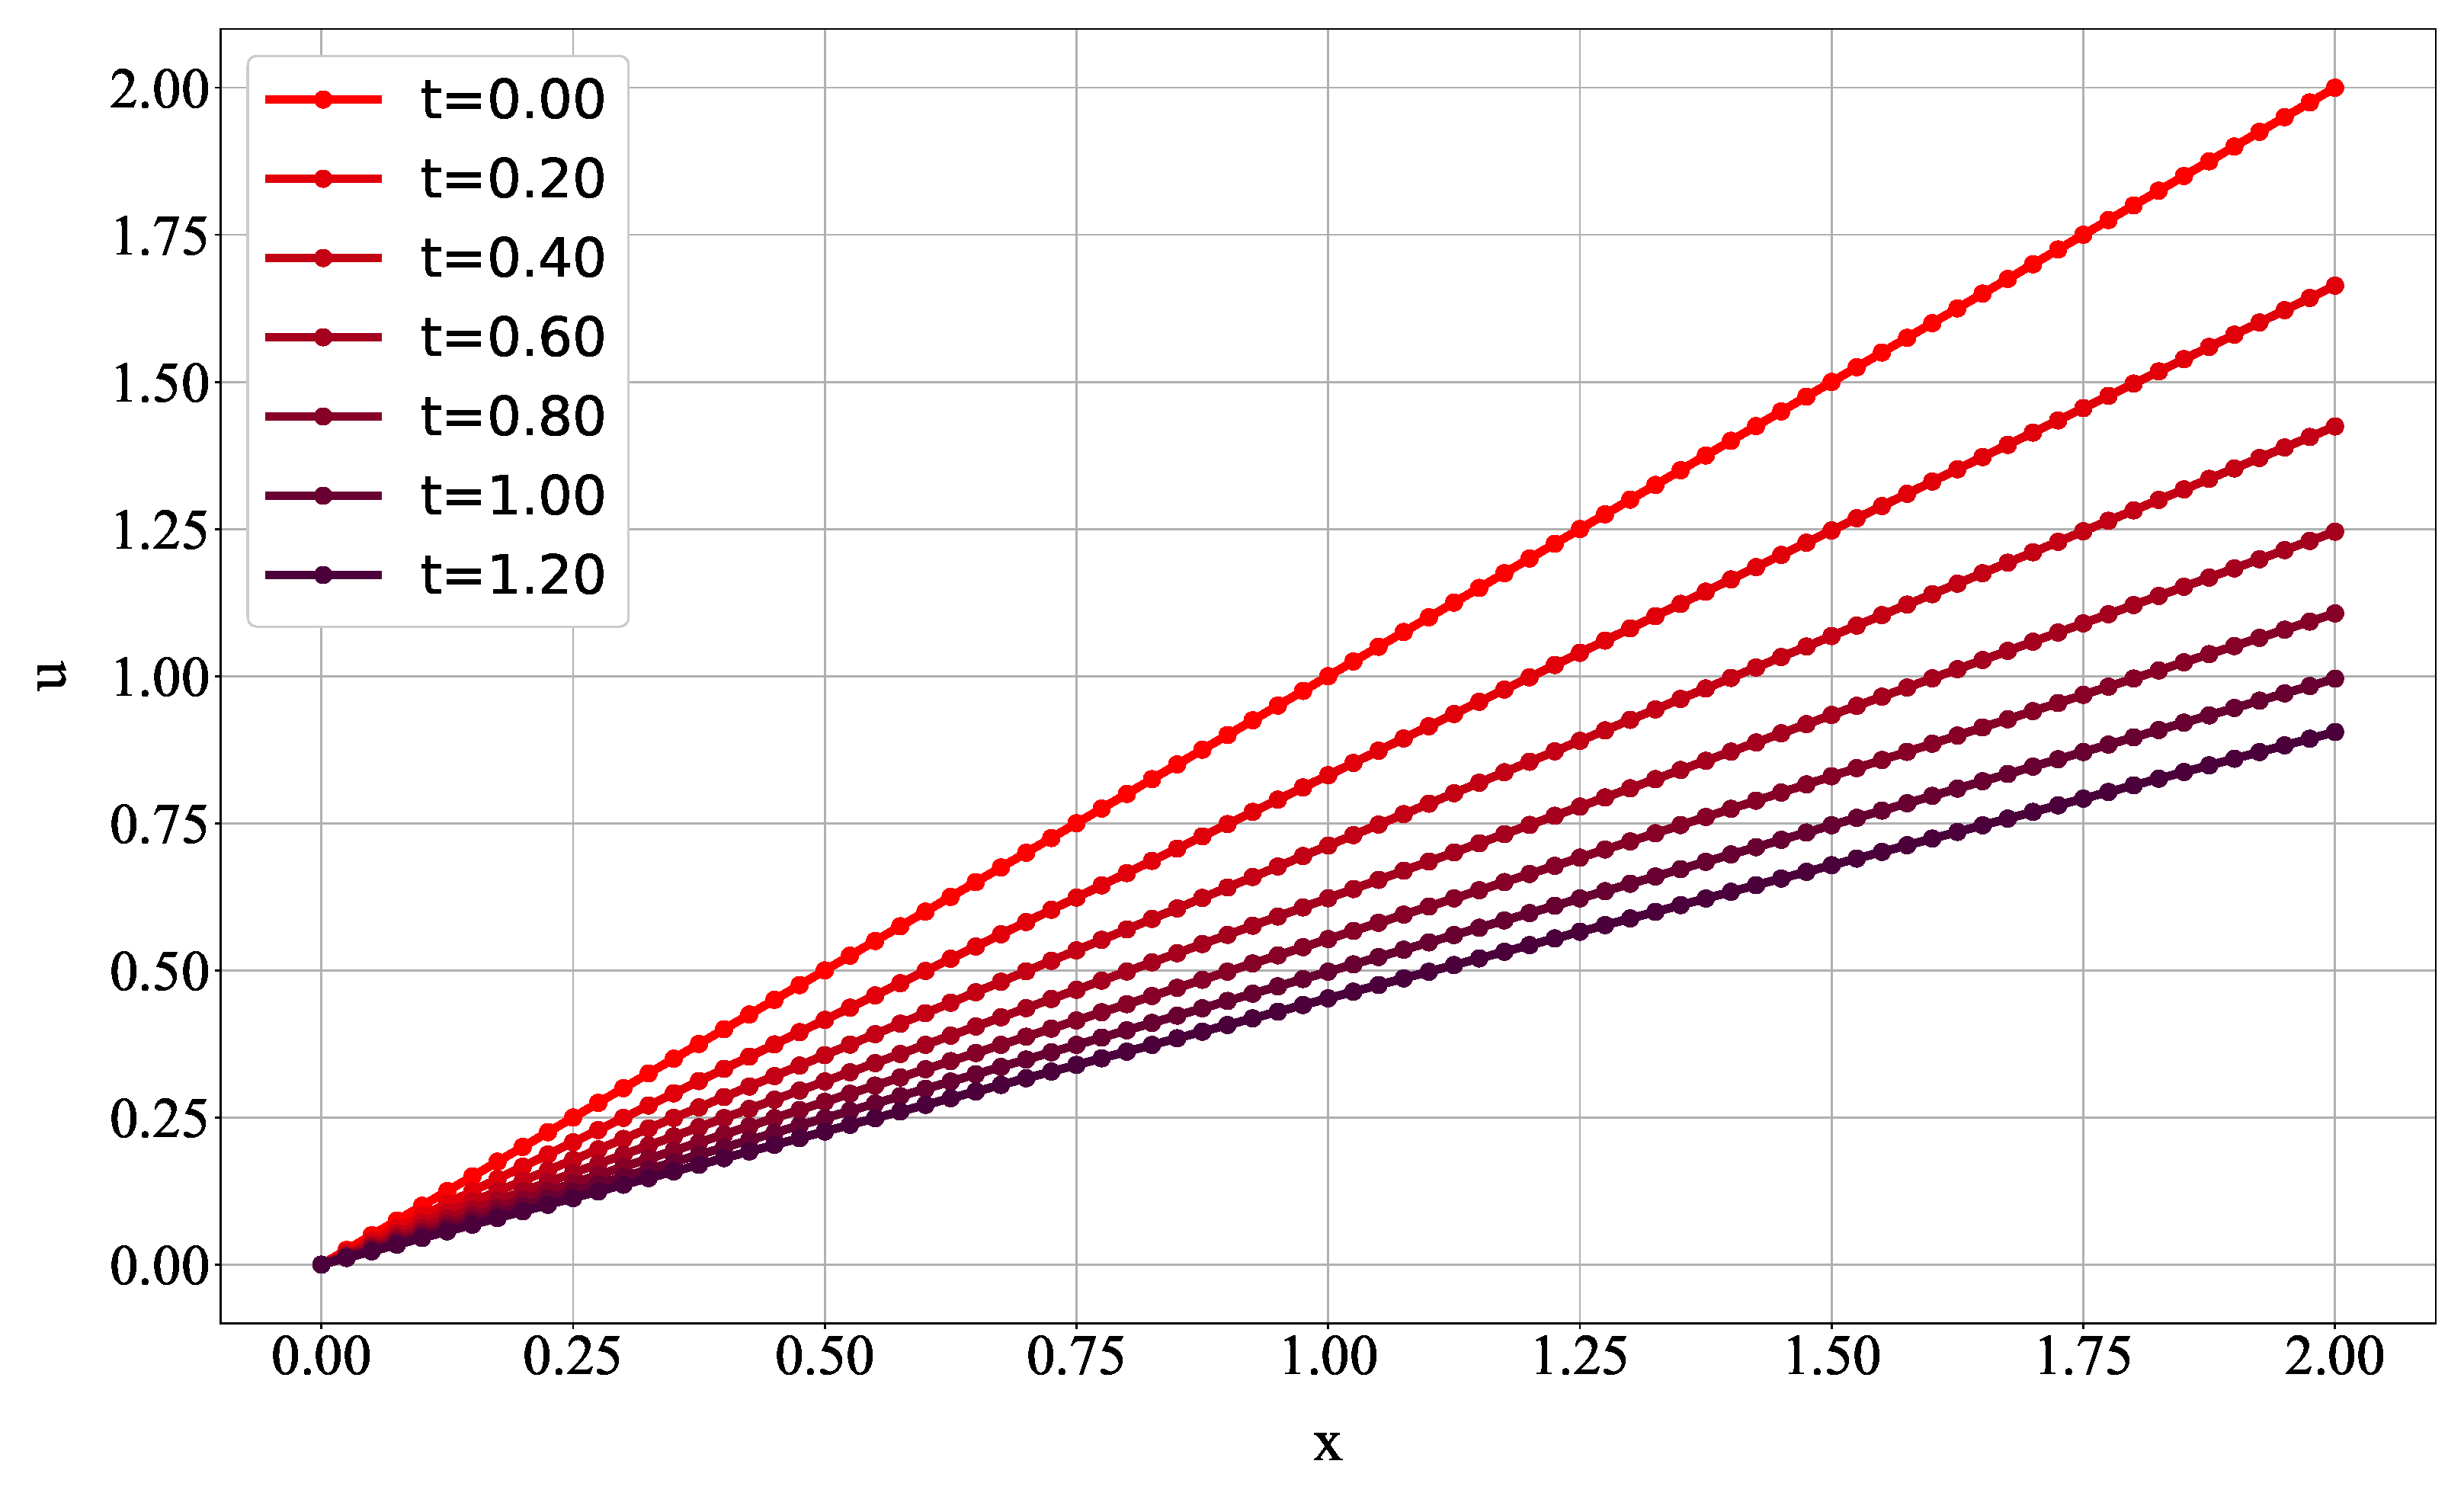
\includegraphics[width=0.425\linewidth]{2.lax.cour05.f2025}}\\
      %\cmidrule{3-4}
      {}                                          & $0.9$    &
        \raisebox{-0.5\totalheight}{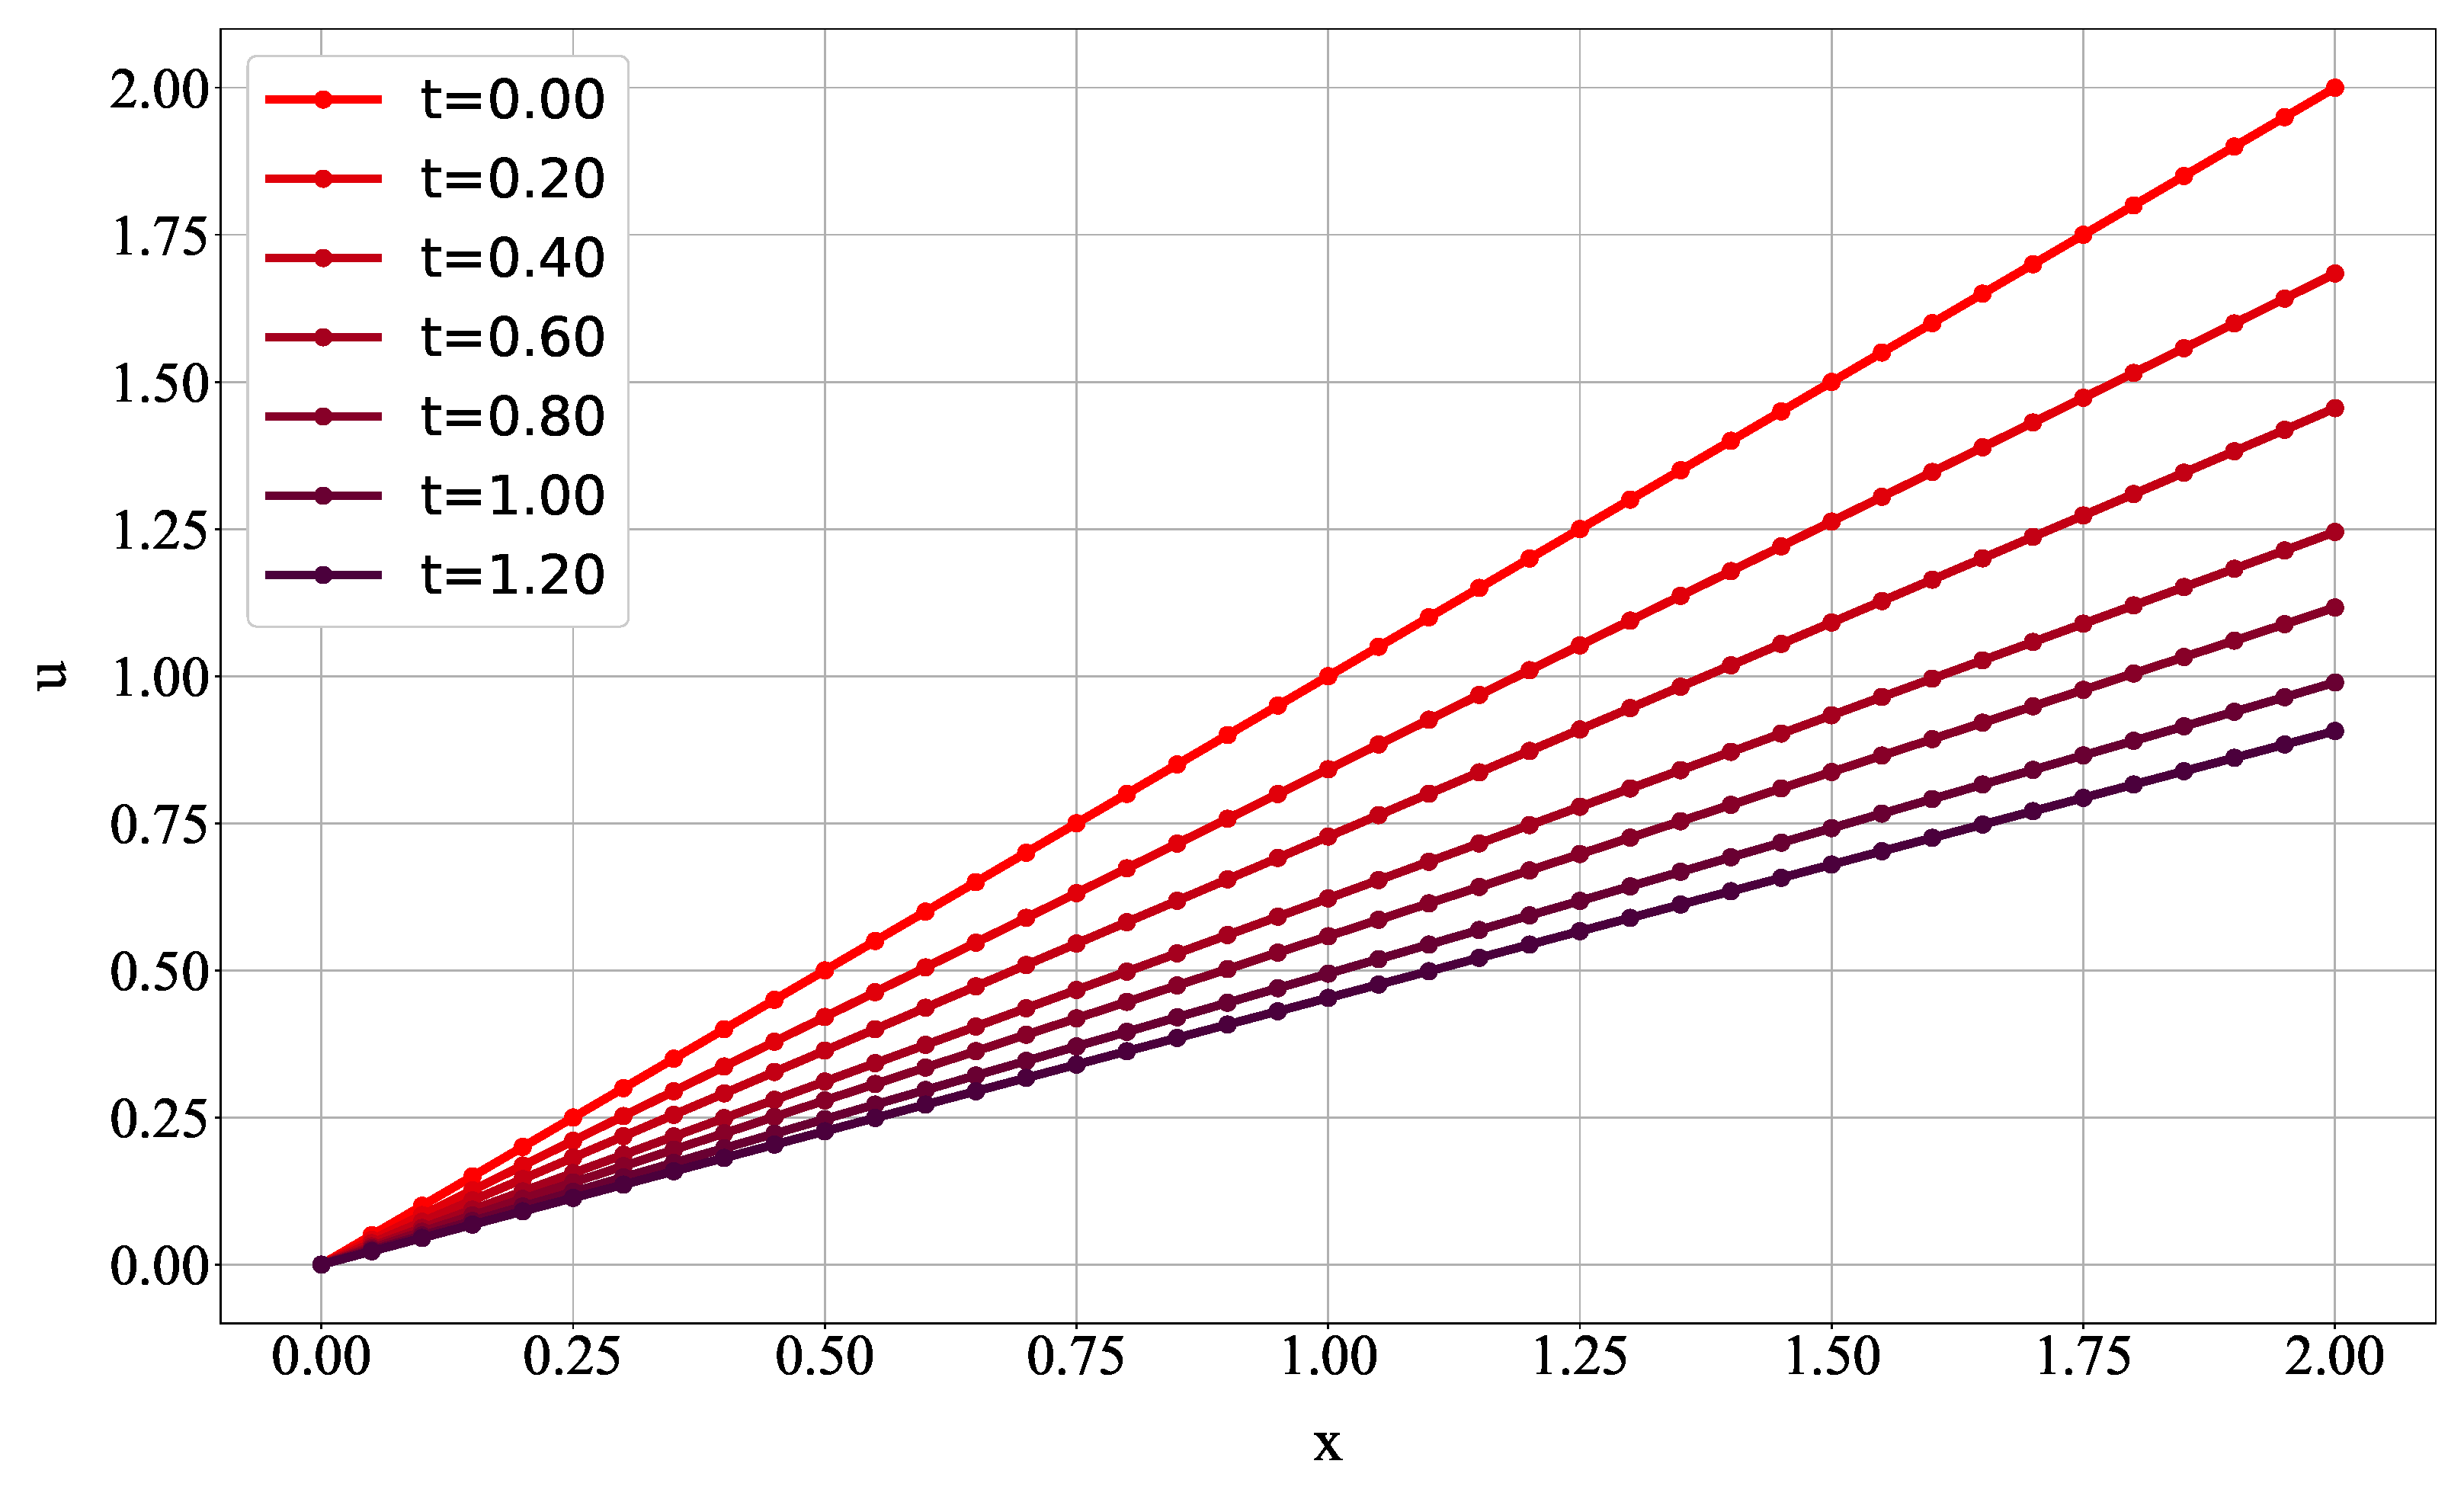
\includegraphics[width=0.425\linewidth]{2.lax.cour09.f2050}} &
        \raisebox{-0.5\totalheight}{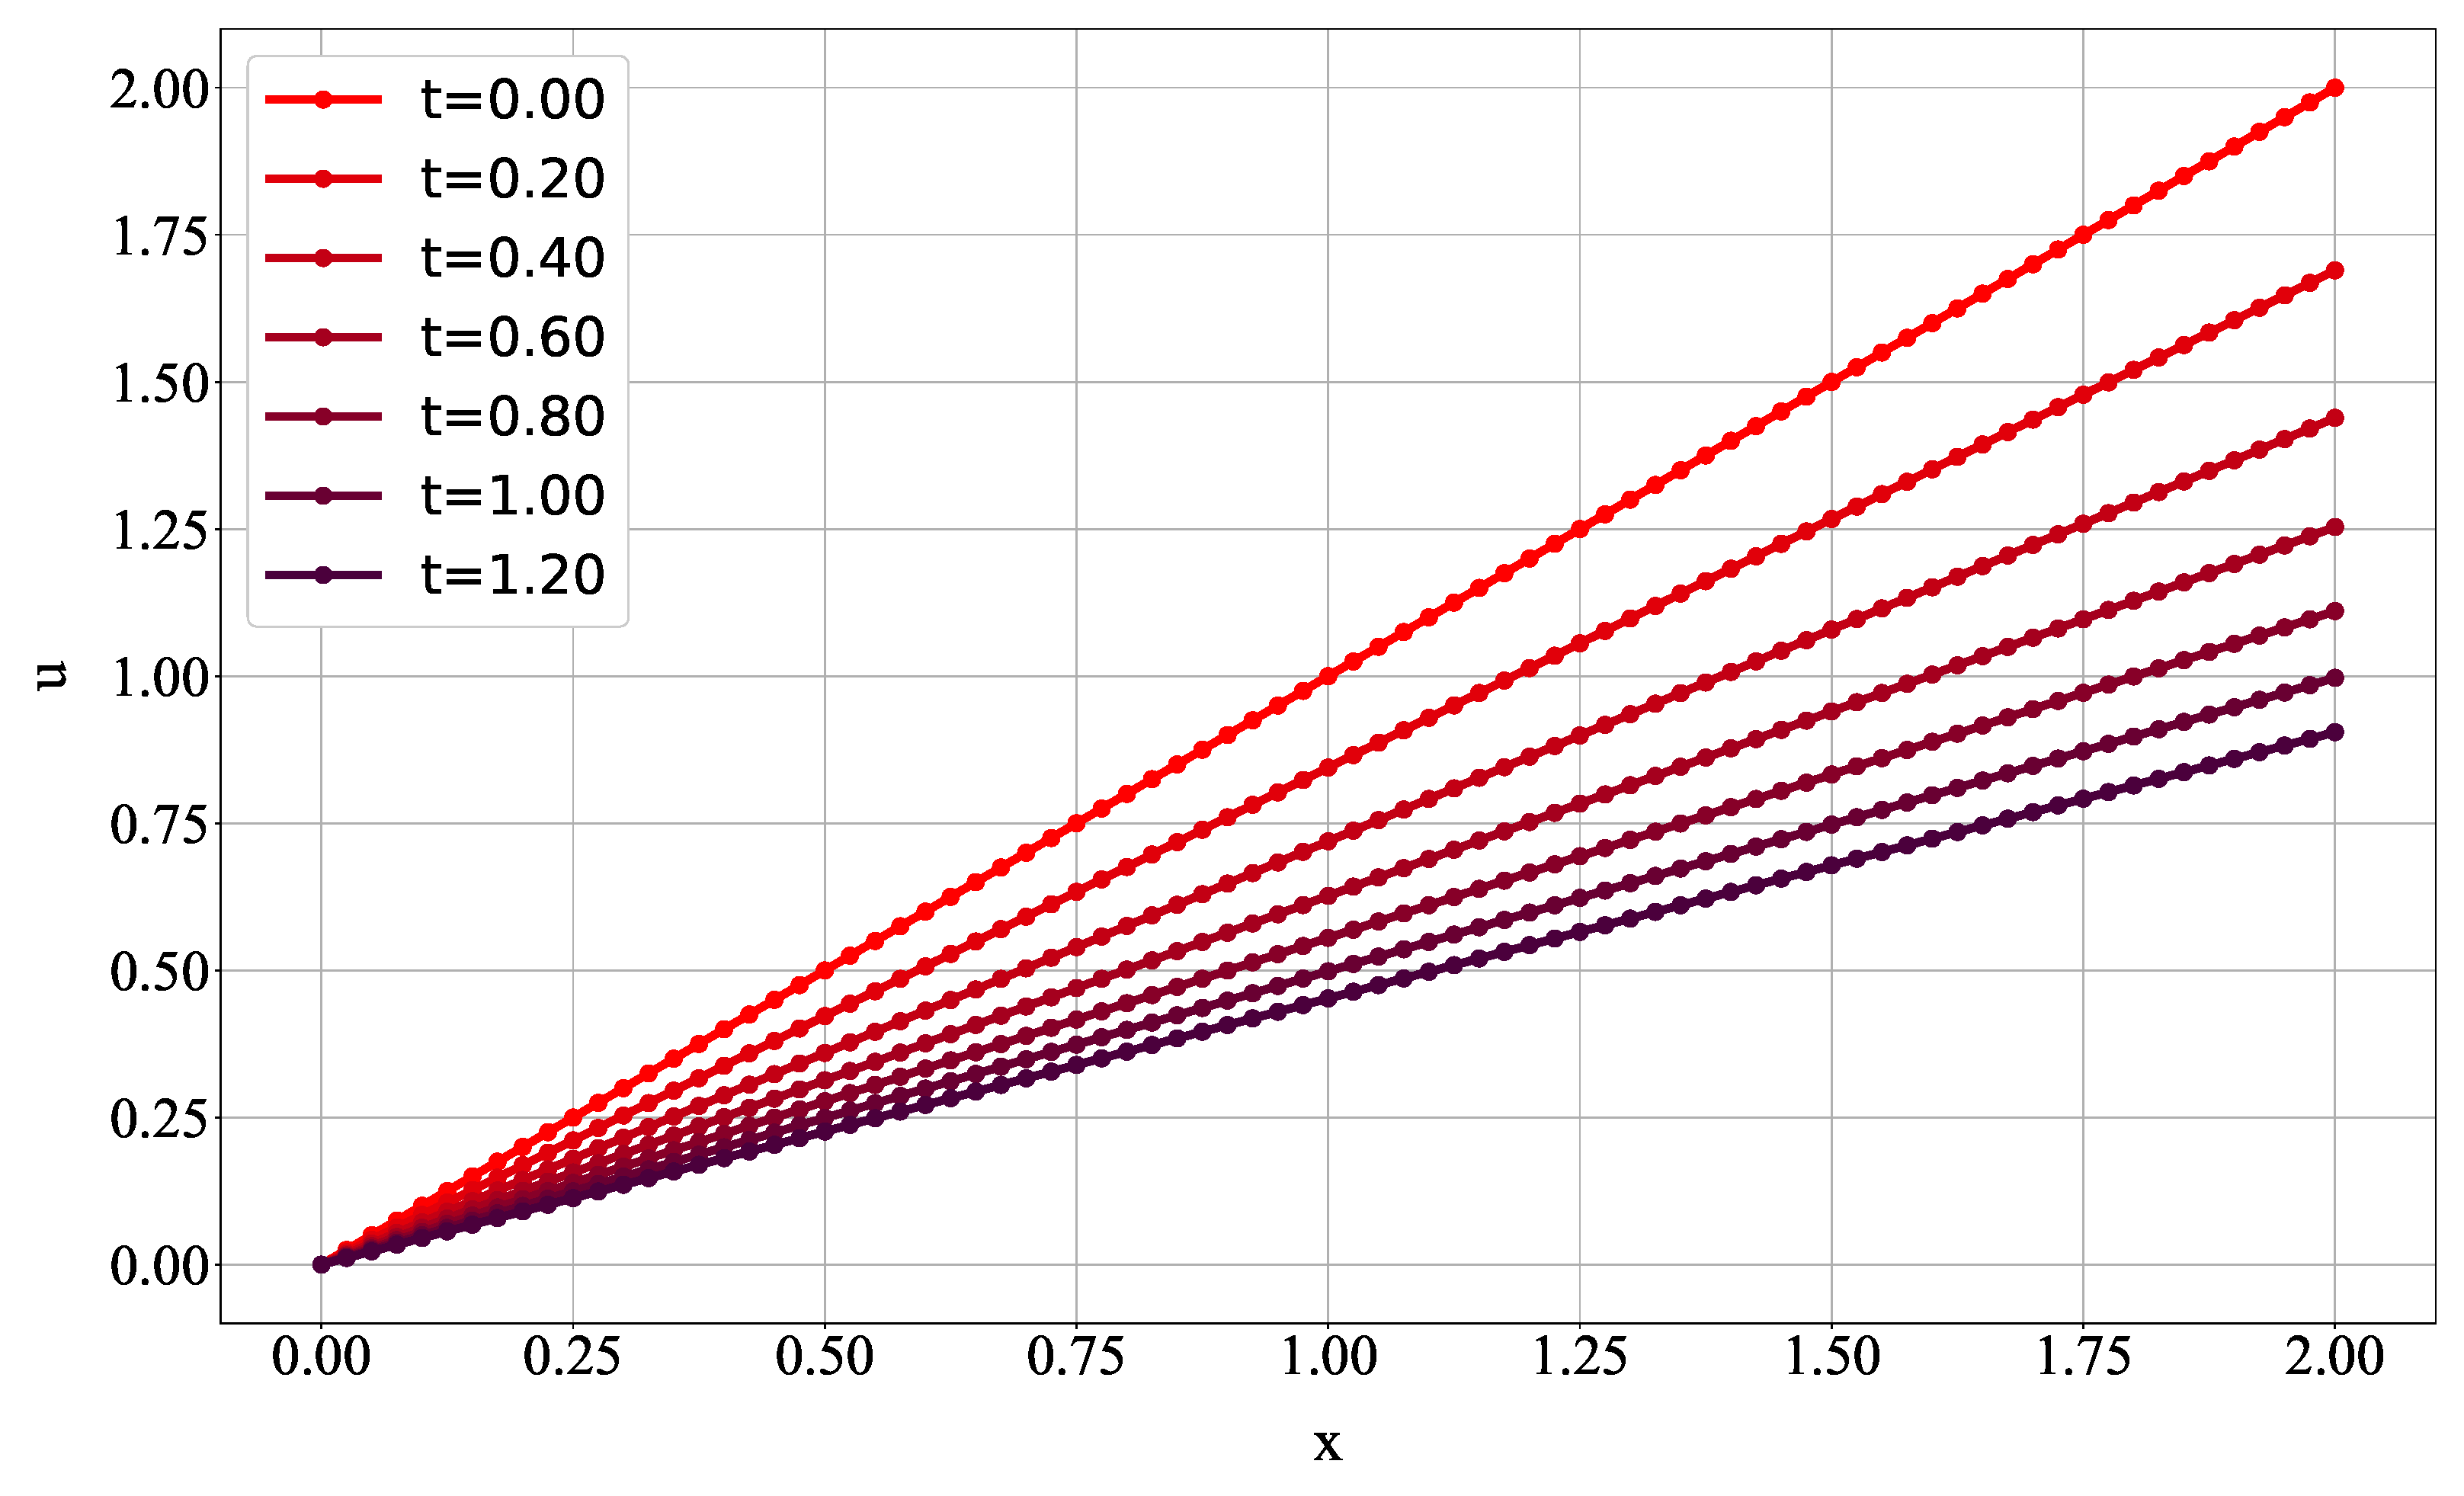
\includegraphics[width=0.425\linewidth]{2.lax.cour09.f2025}}\\
      \bottomrule
    \end{tabular}
  \end{center}
  \end{table}
  
  \begin{table}[p]
  \caption{"`Курант-Изаксон-Рис"' (\ref{sec:cir})}
  \label{plot:cir}
  \begin{center}
    \begin{tabular}{c c c c}
      \toprule
      {$f$}                                       & $\sigma$ & $h_1$ & $h_2$\\
      \midrule
      \multirow{2}{*}{\vspace{\myvspaceOne}$f_1$} & $0.5$    & 
        \raisebox{-0.5\totalheight}{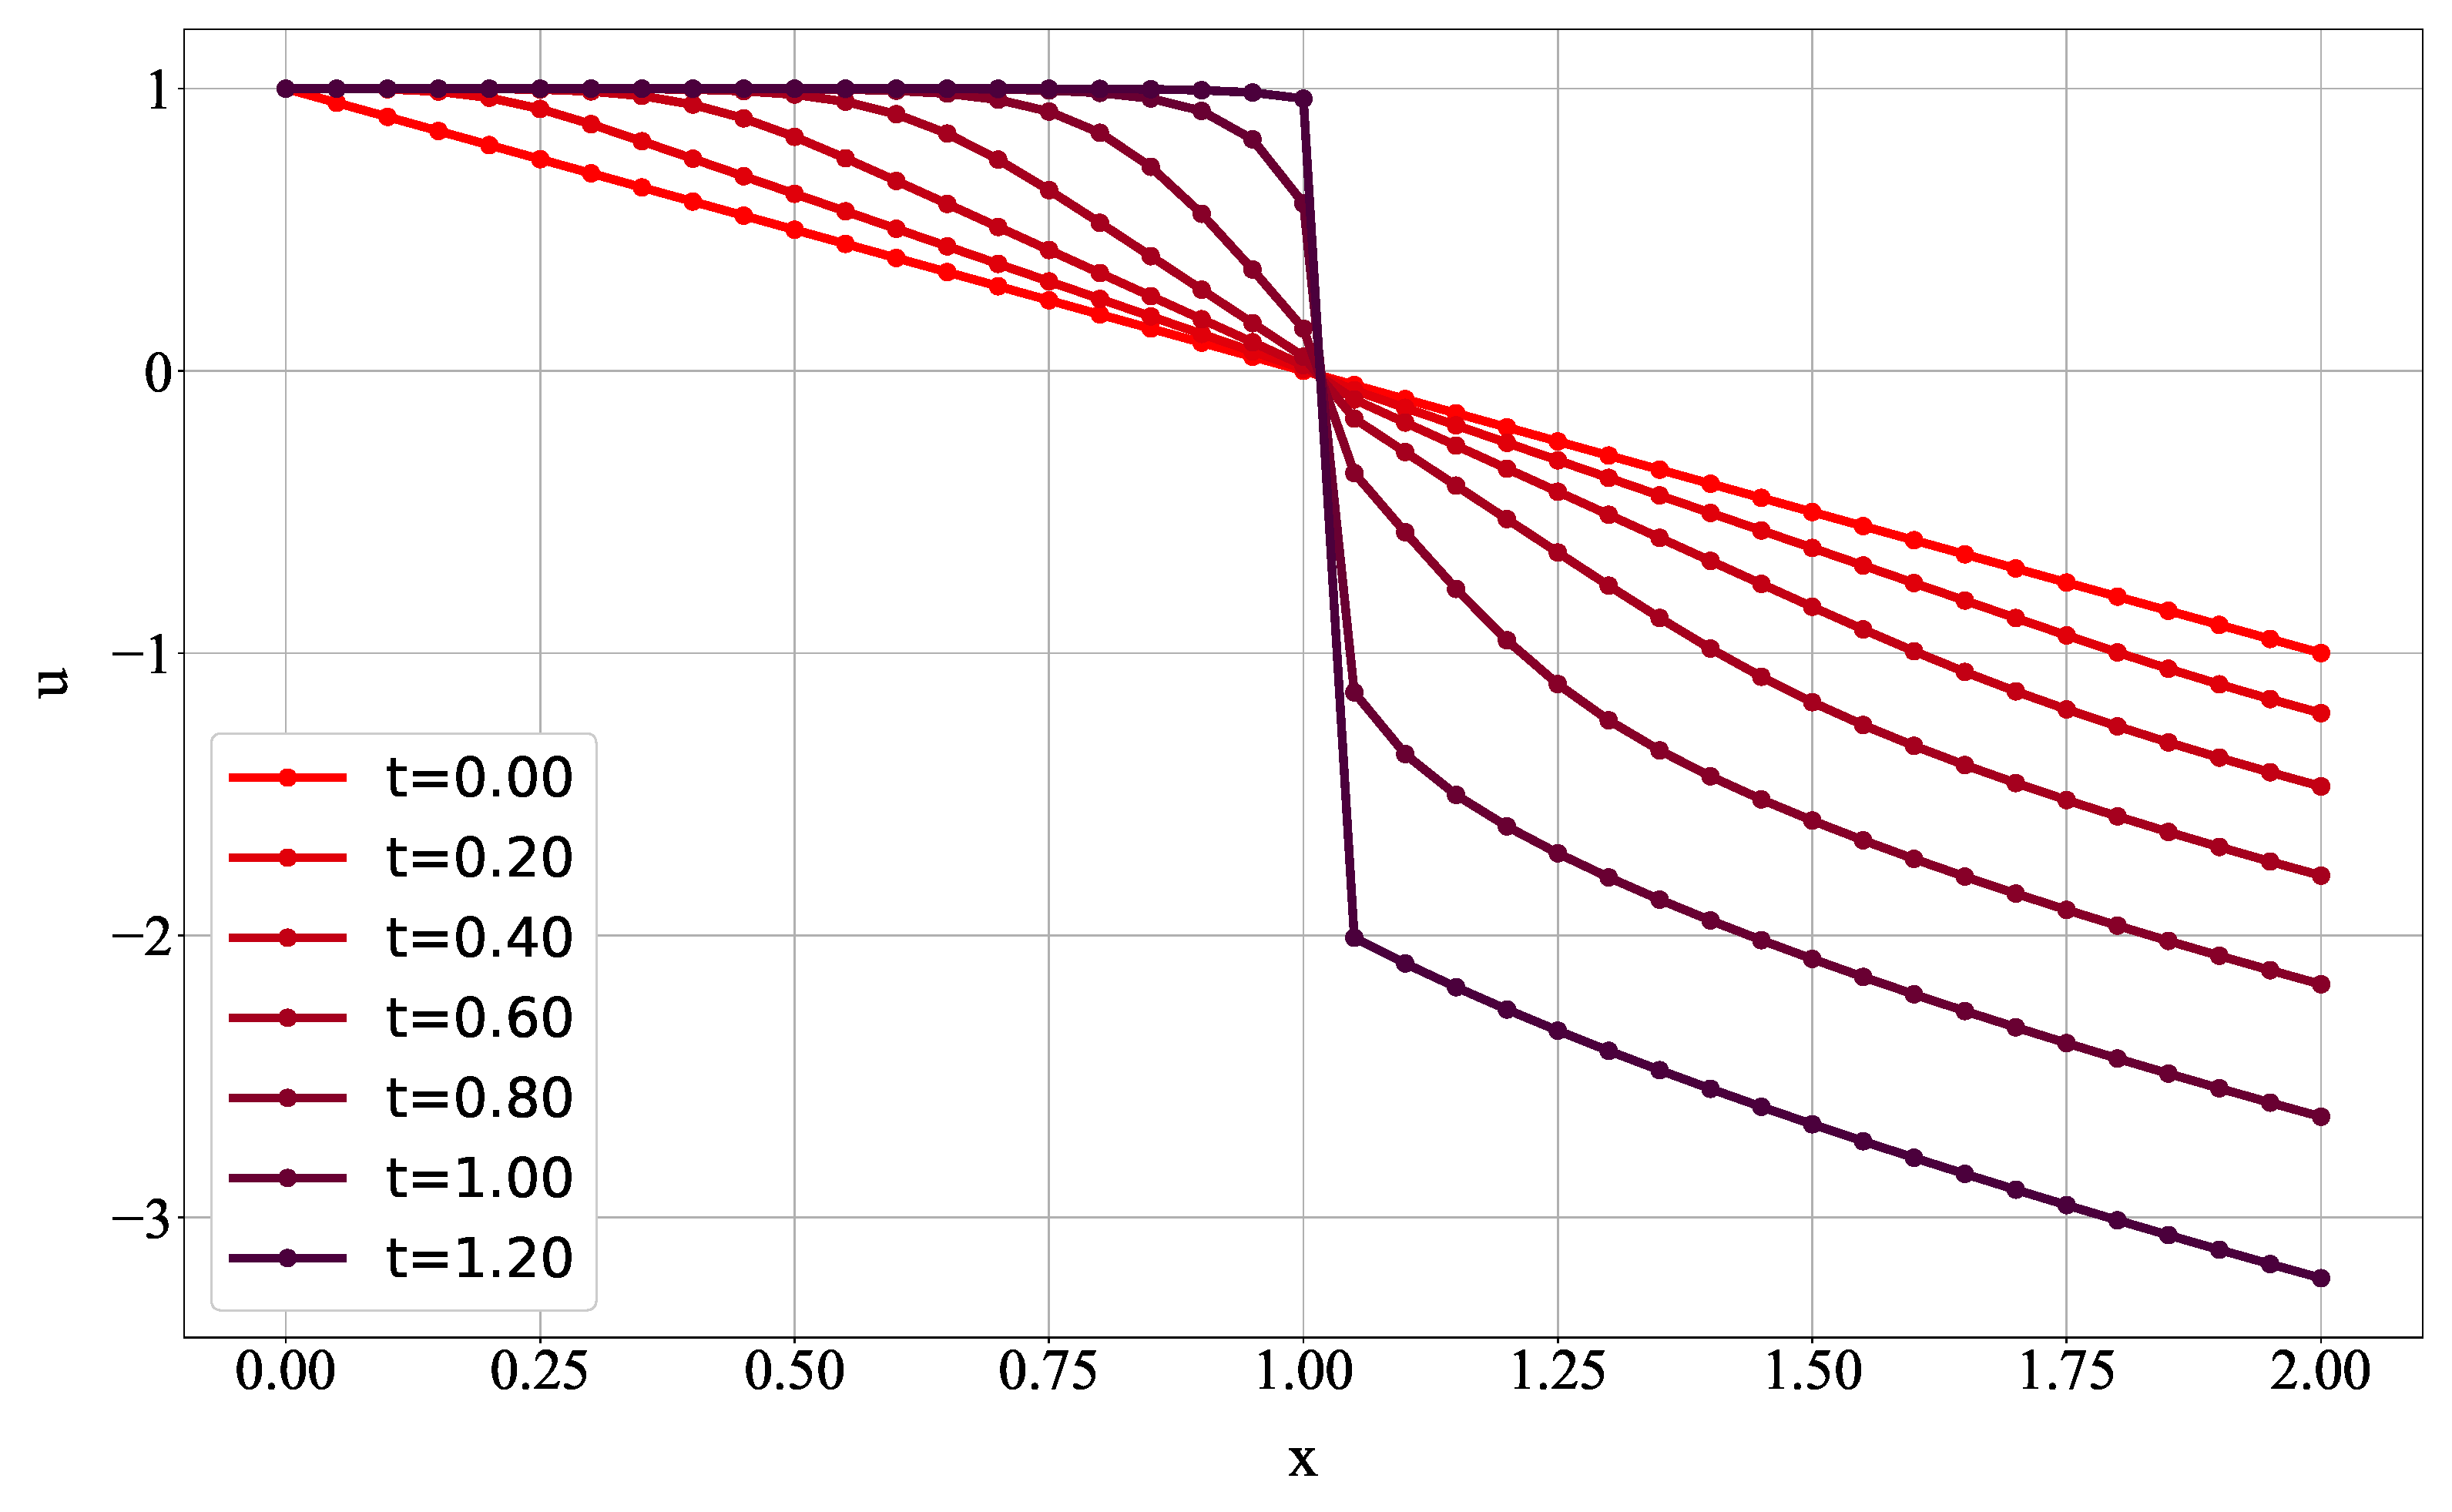
\includegraphics[width=0.425\linewidth]{3.cir.cour05.f1050}} &
        \raisebox{-0.5\totalheight}{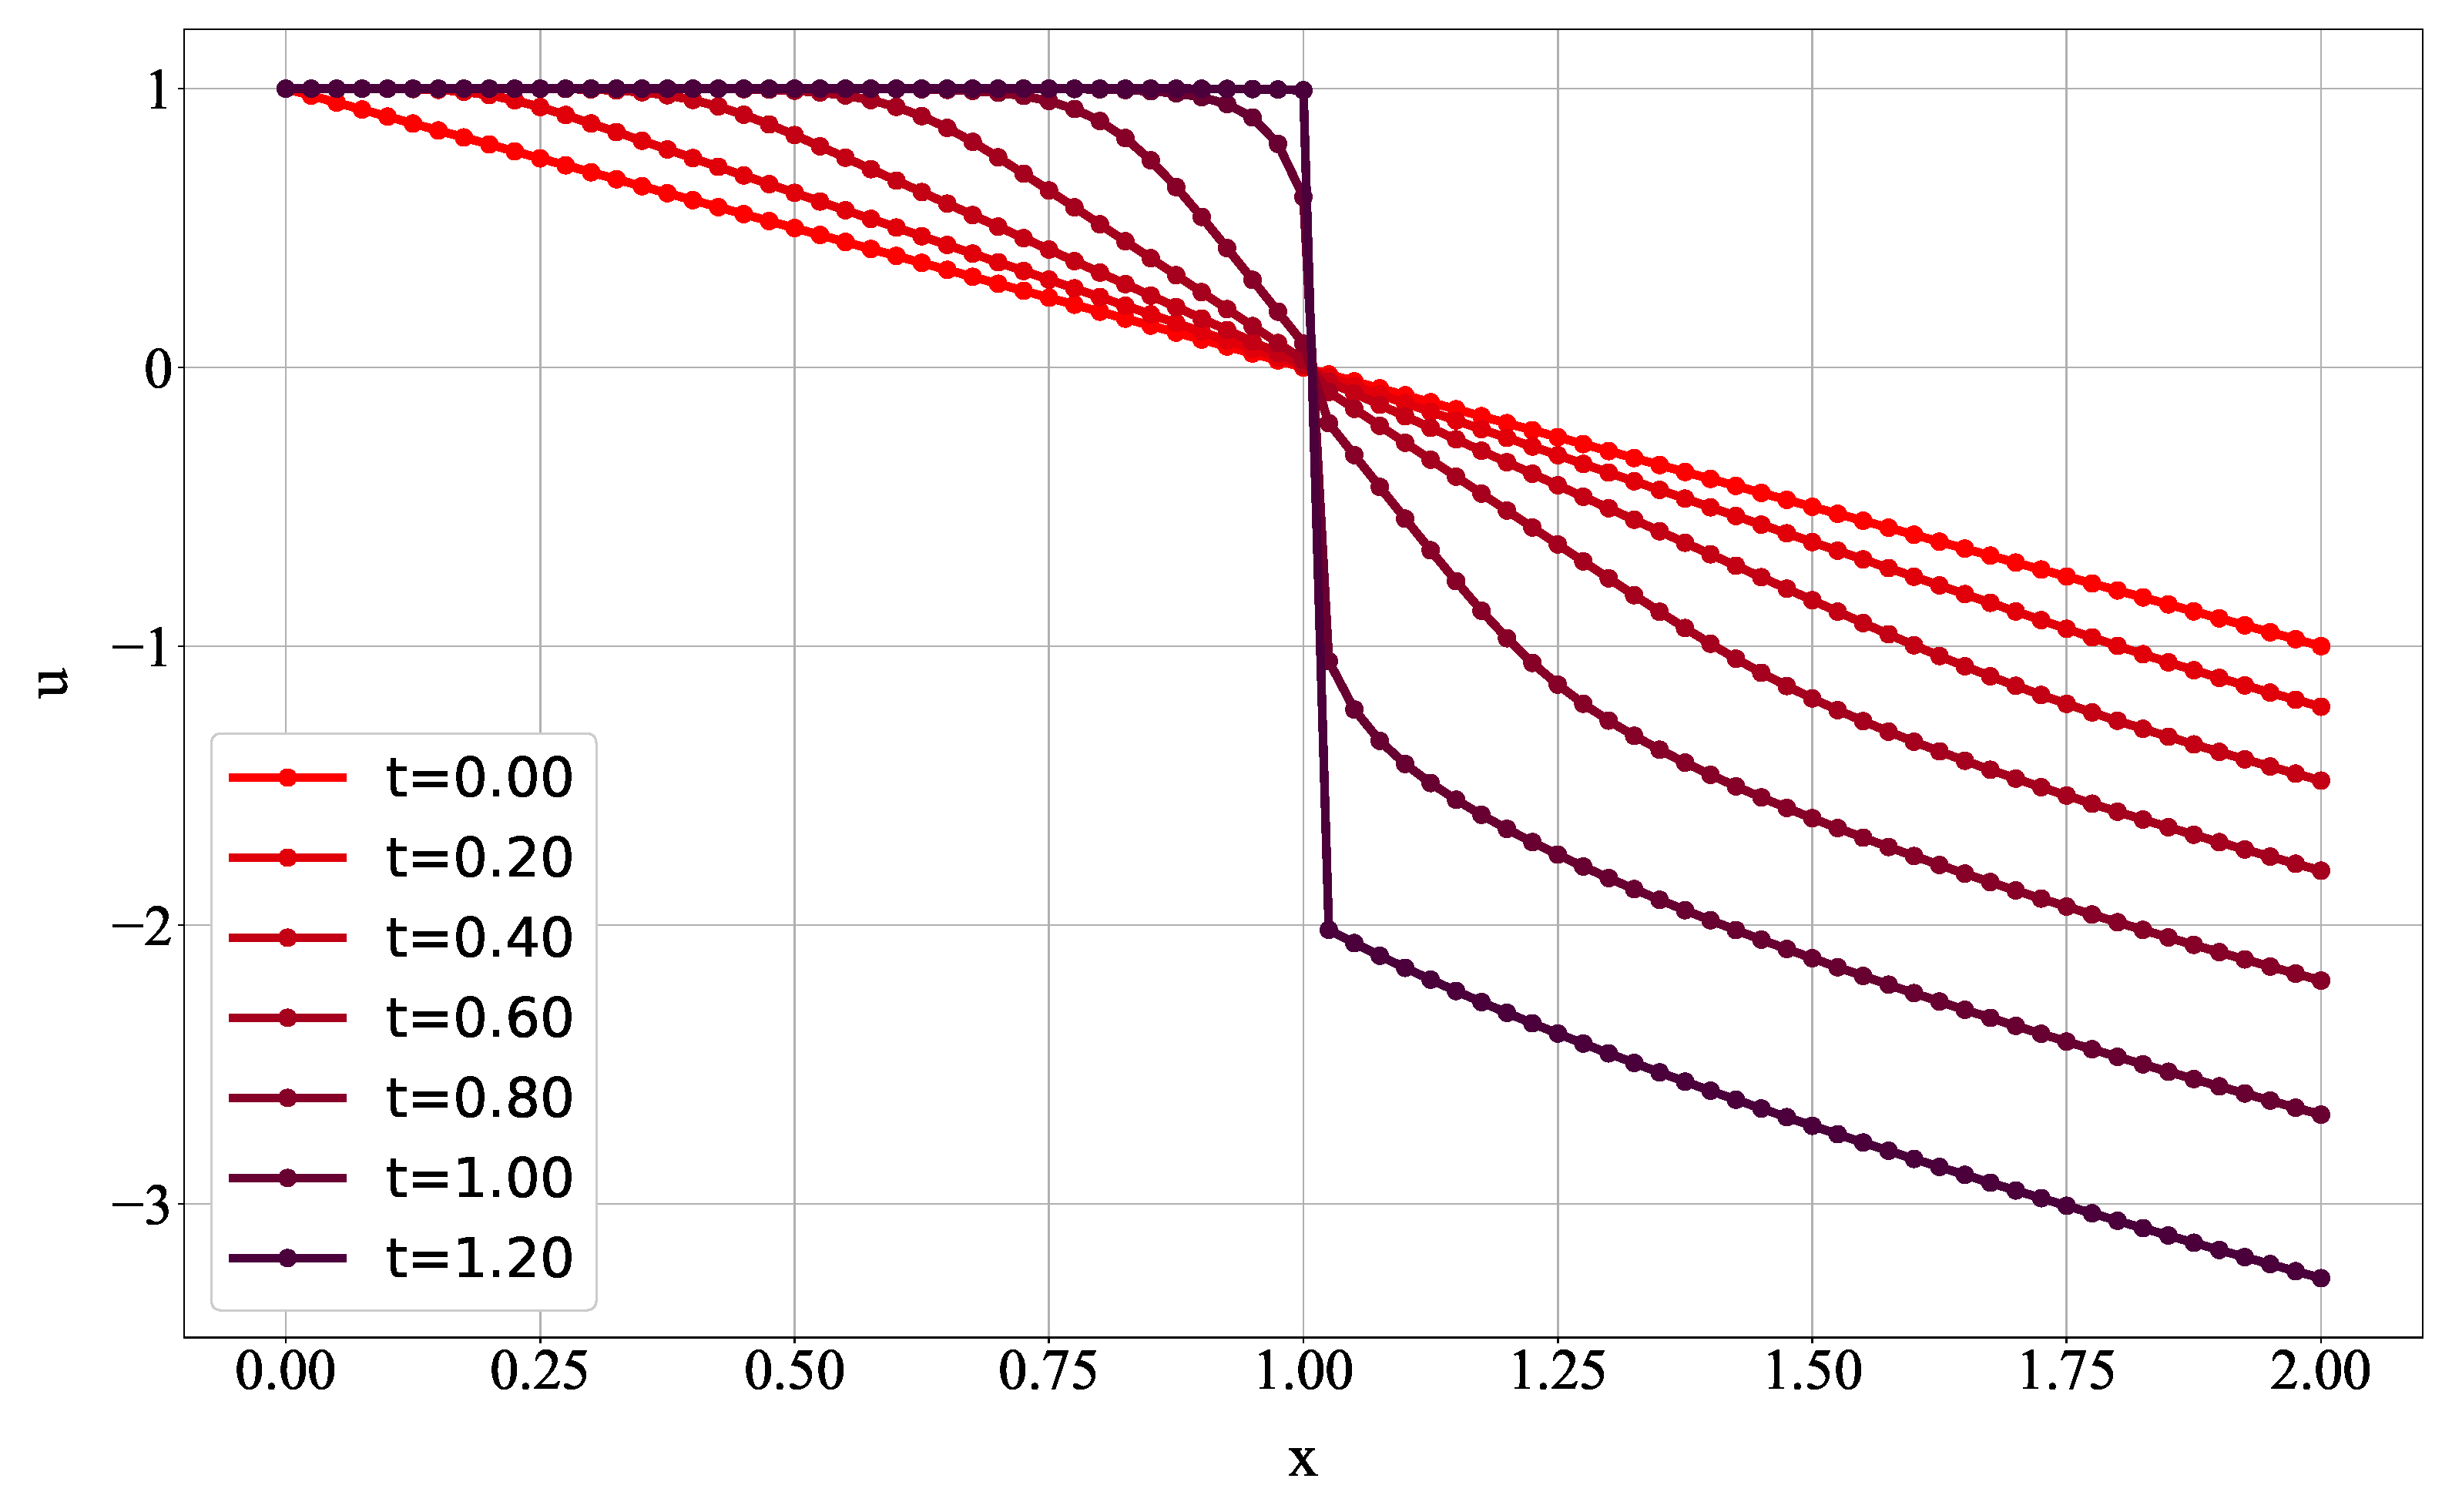
\includegraphics[width=0.425\linewidth]{3.cir.cour05.f1025}}\\
      %\cmidrule{3-4}
      {}                                          & $0.9$    &
        \raisebox{-0.5\totalheight}{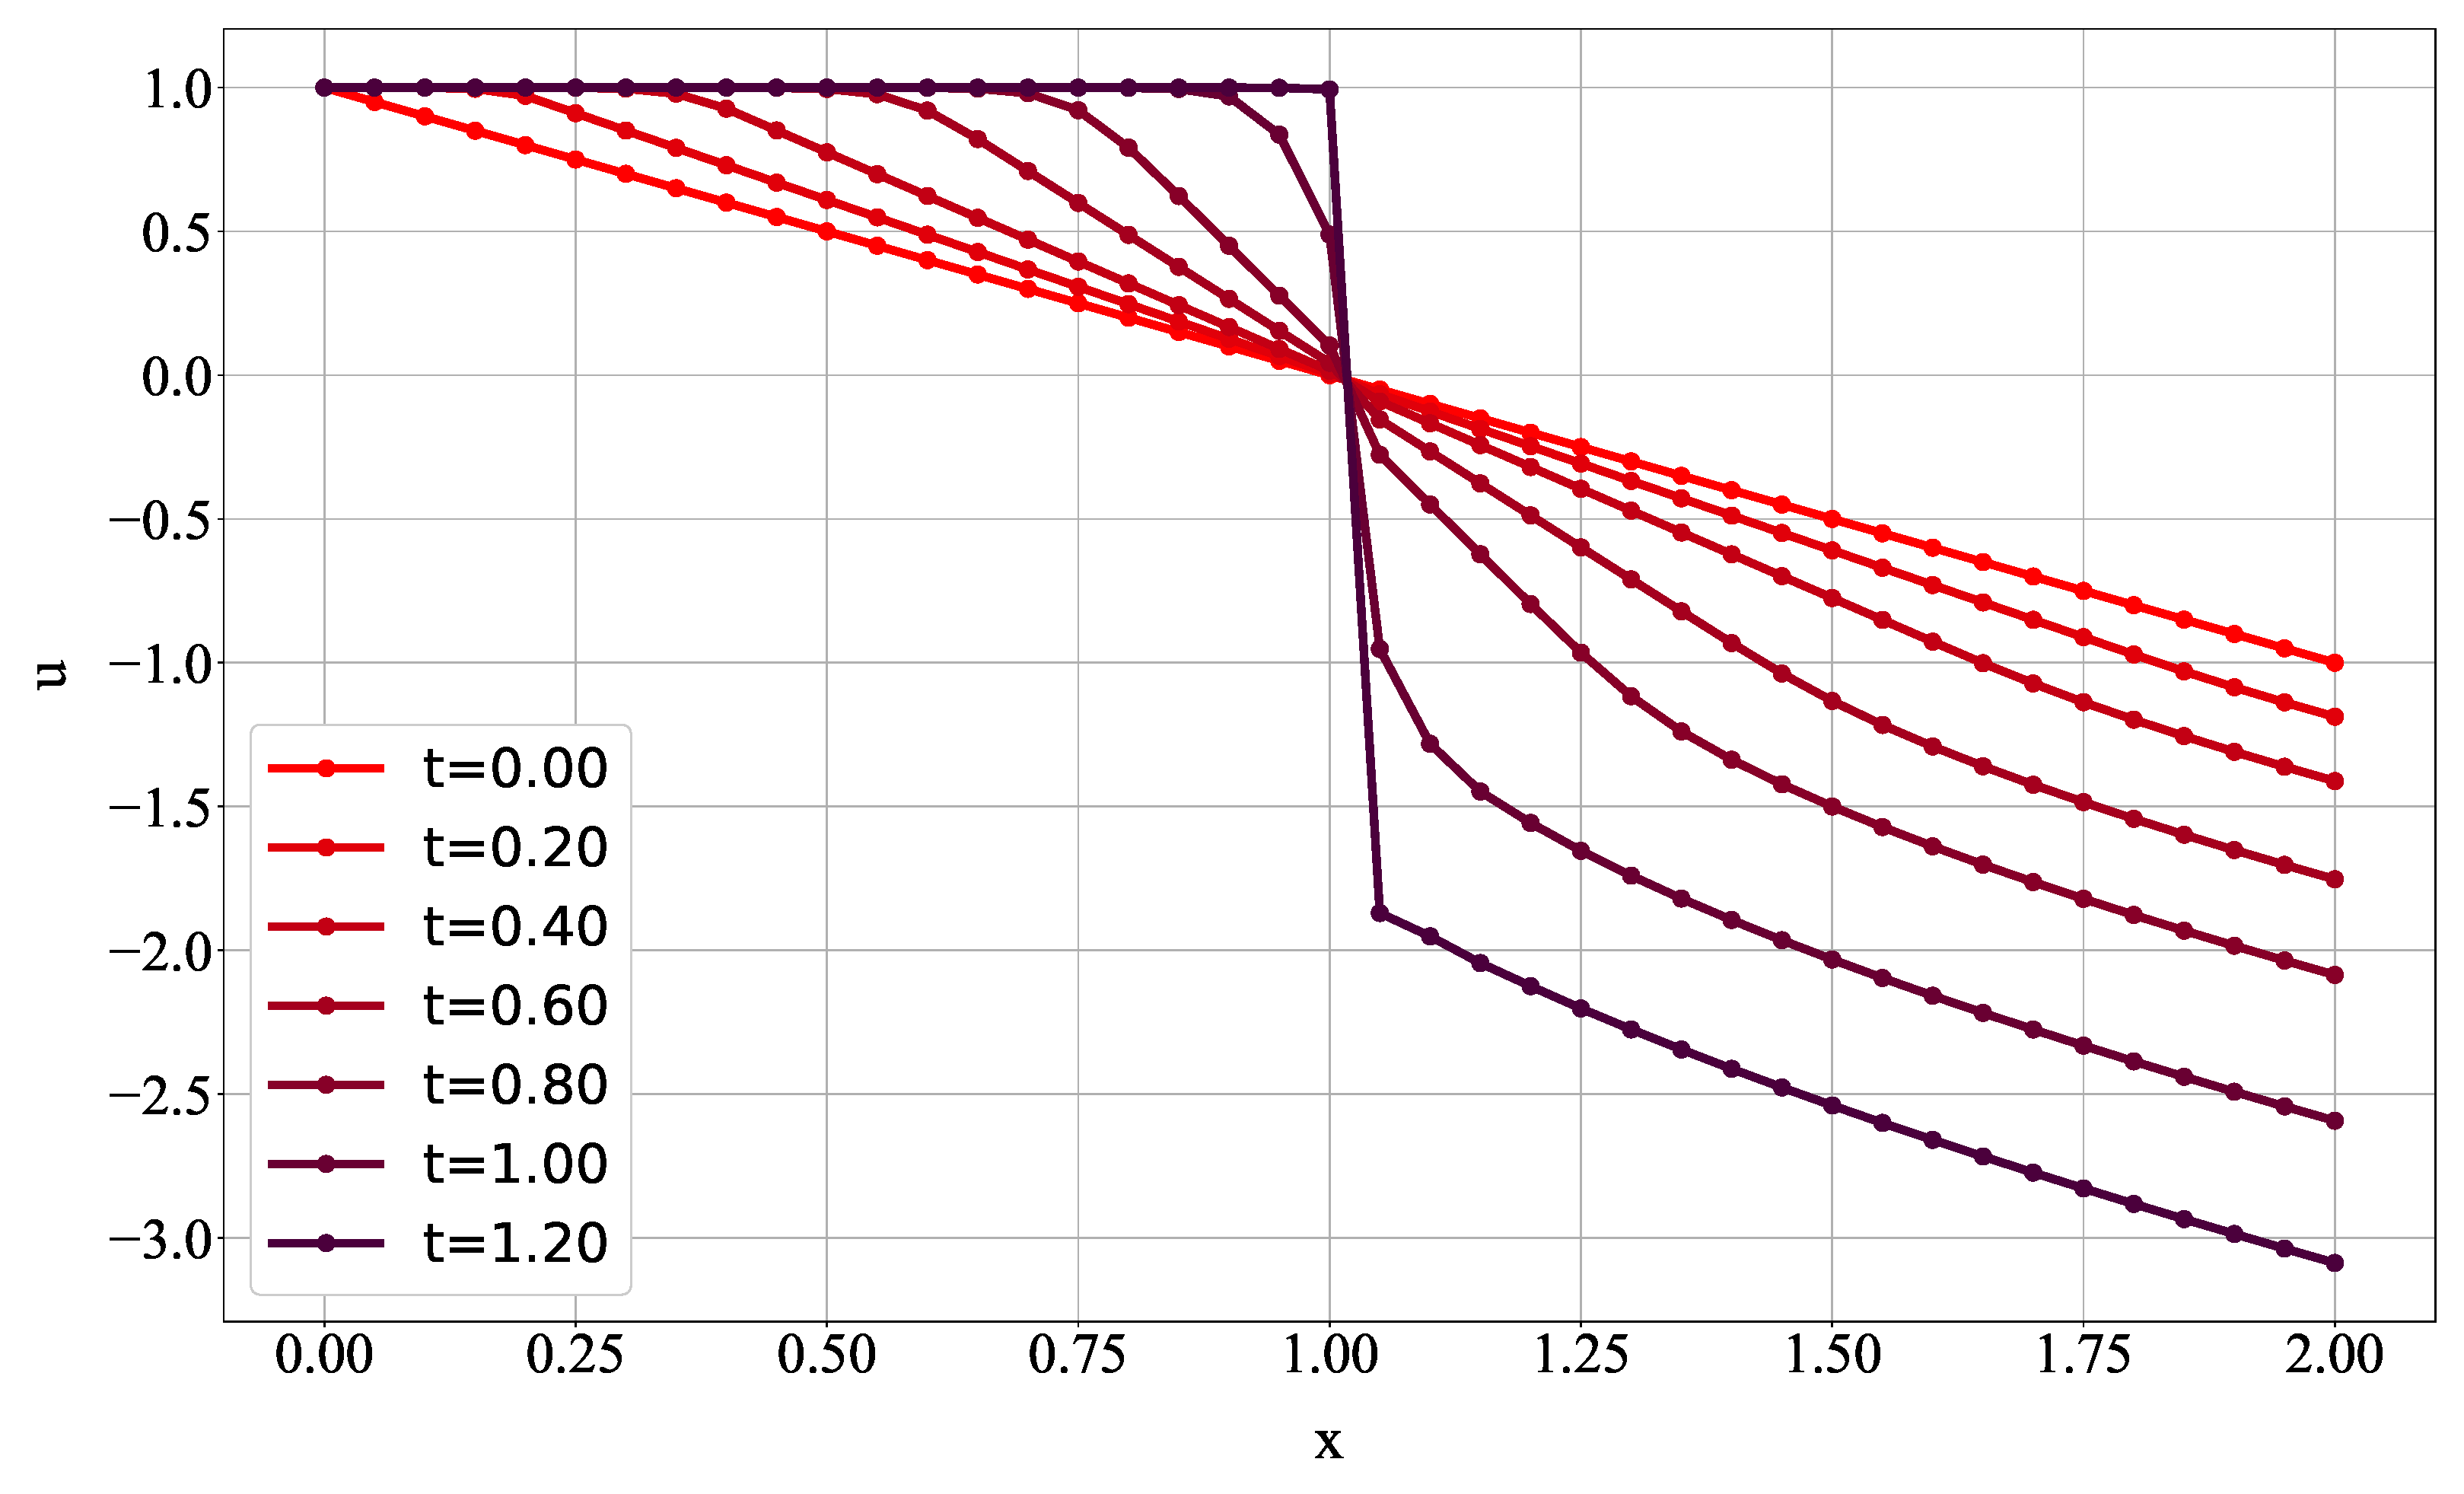
\includegraphics[width=0.425\linewidth]{3.cir.cour09.f1050}} & 
        \raisebox{-0.5\totalheight}{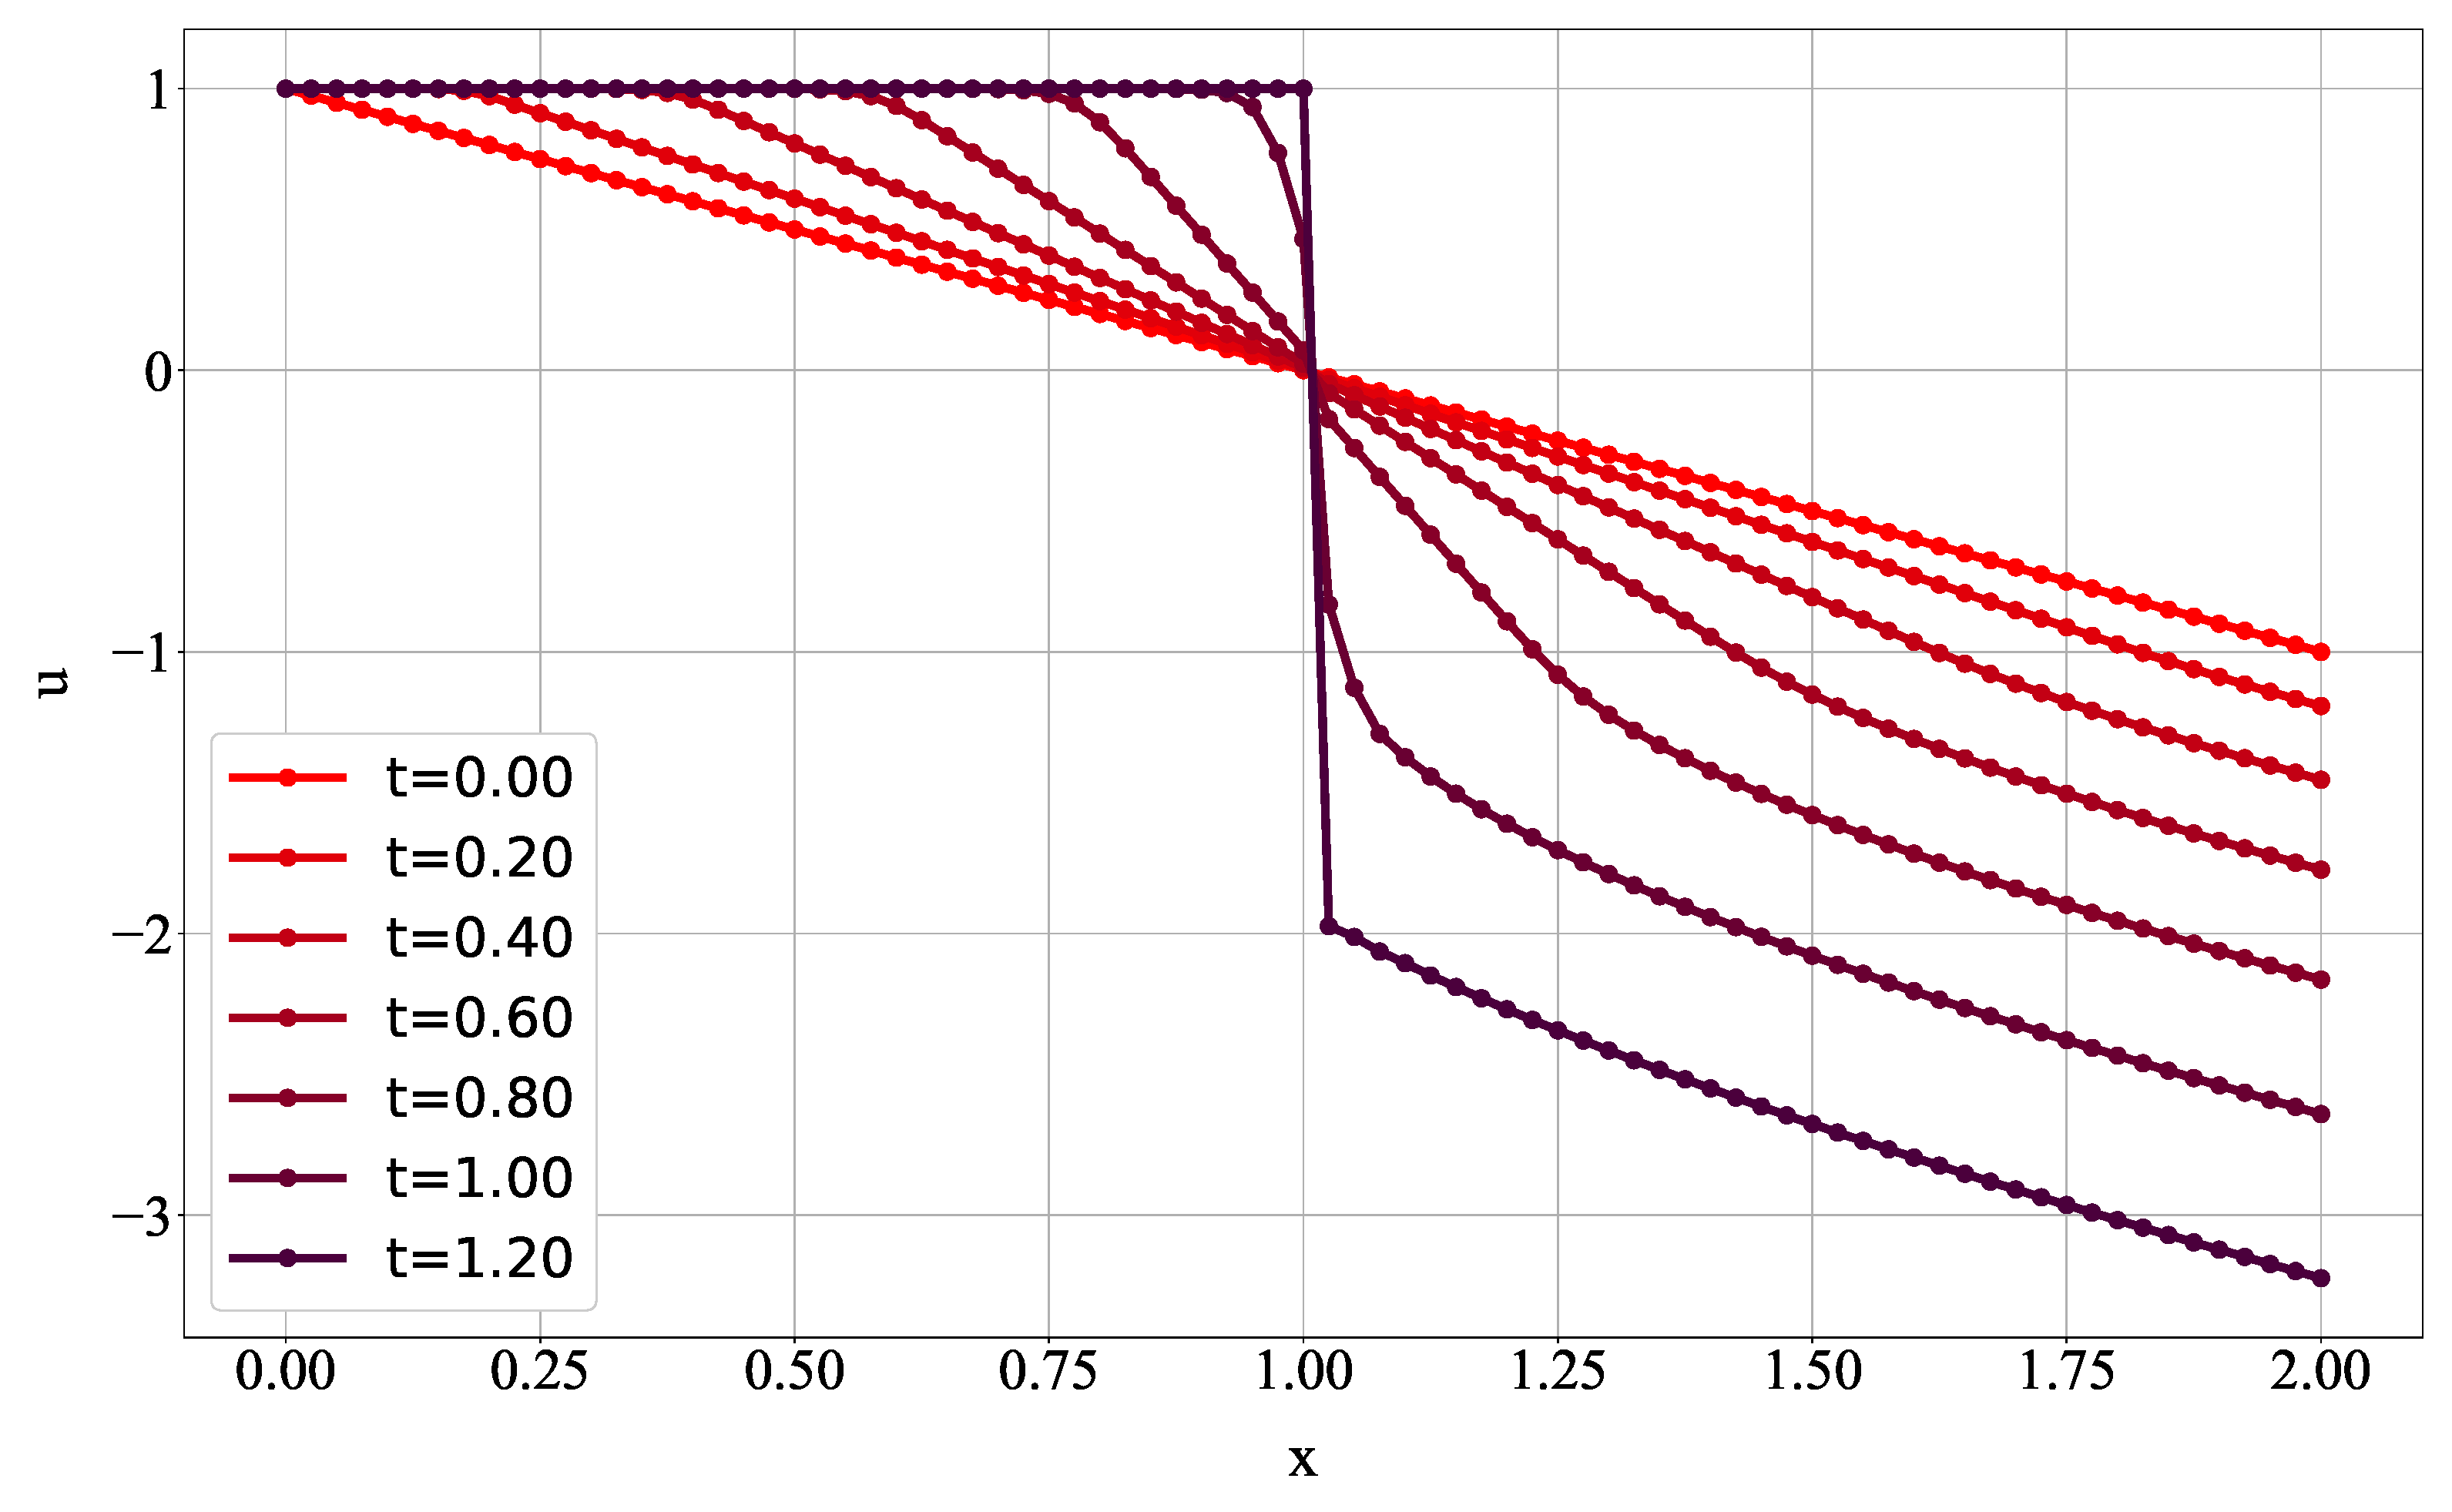
\includegraphics[width=0.425\linewidth]{3.cir.cour09.f1025}}\\
      \midrule
      \multirow{2}{*}{\vspace{\myvspaceOne}$f_2$} & $0.5$    &
        \raisebox{-0.5\totalheight}{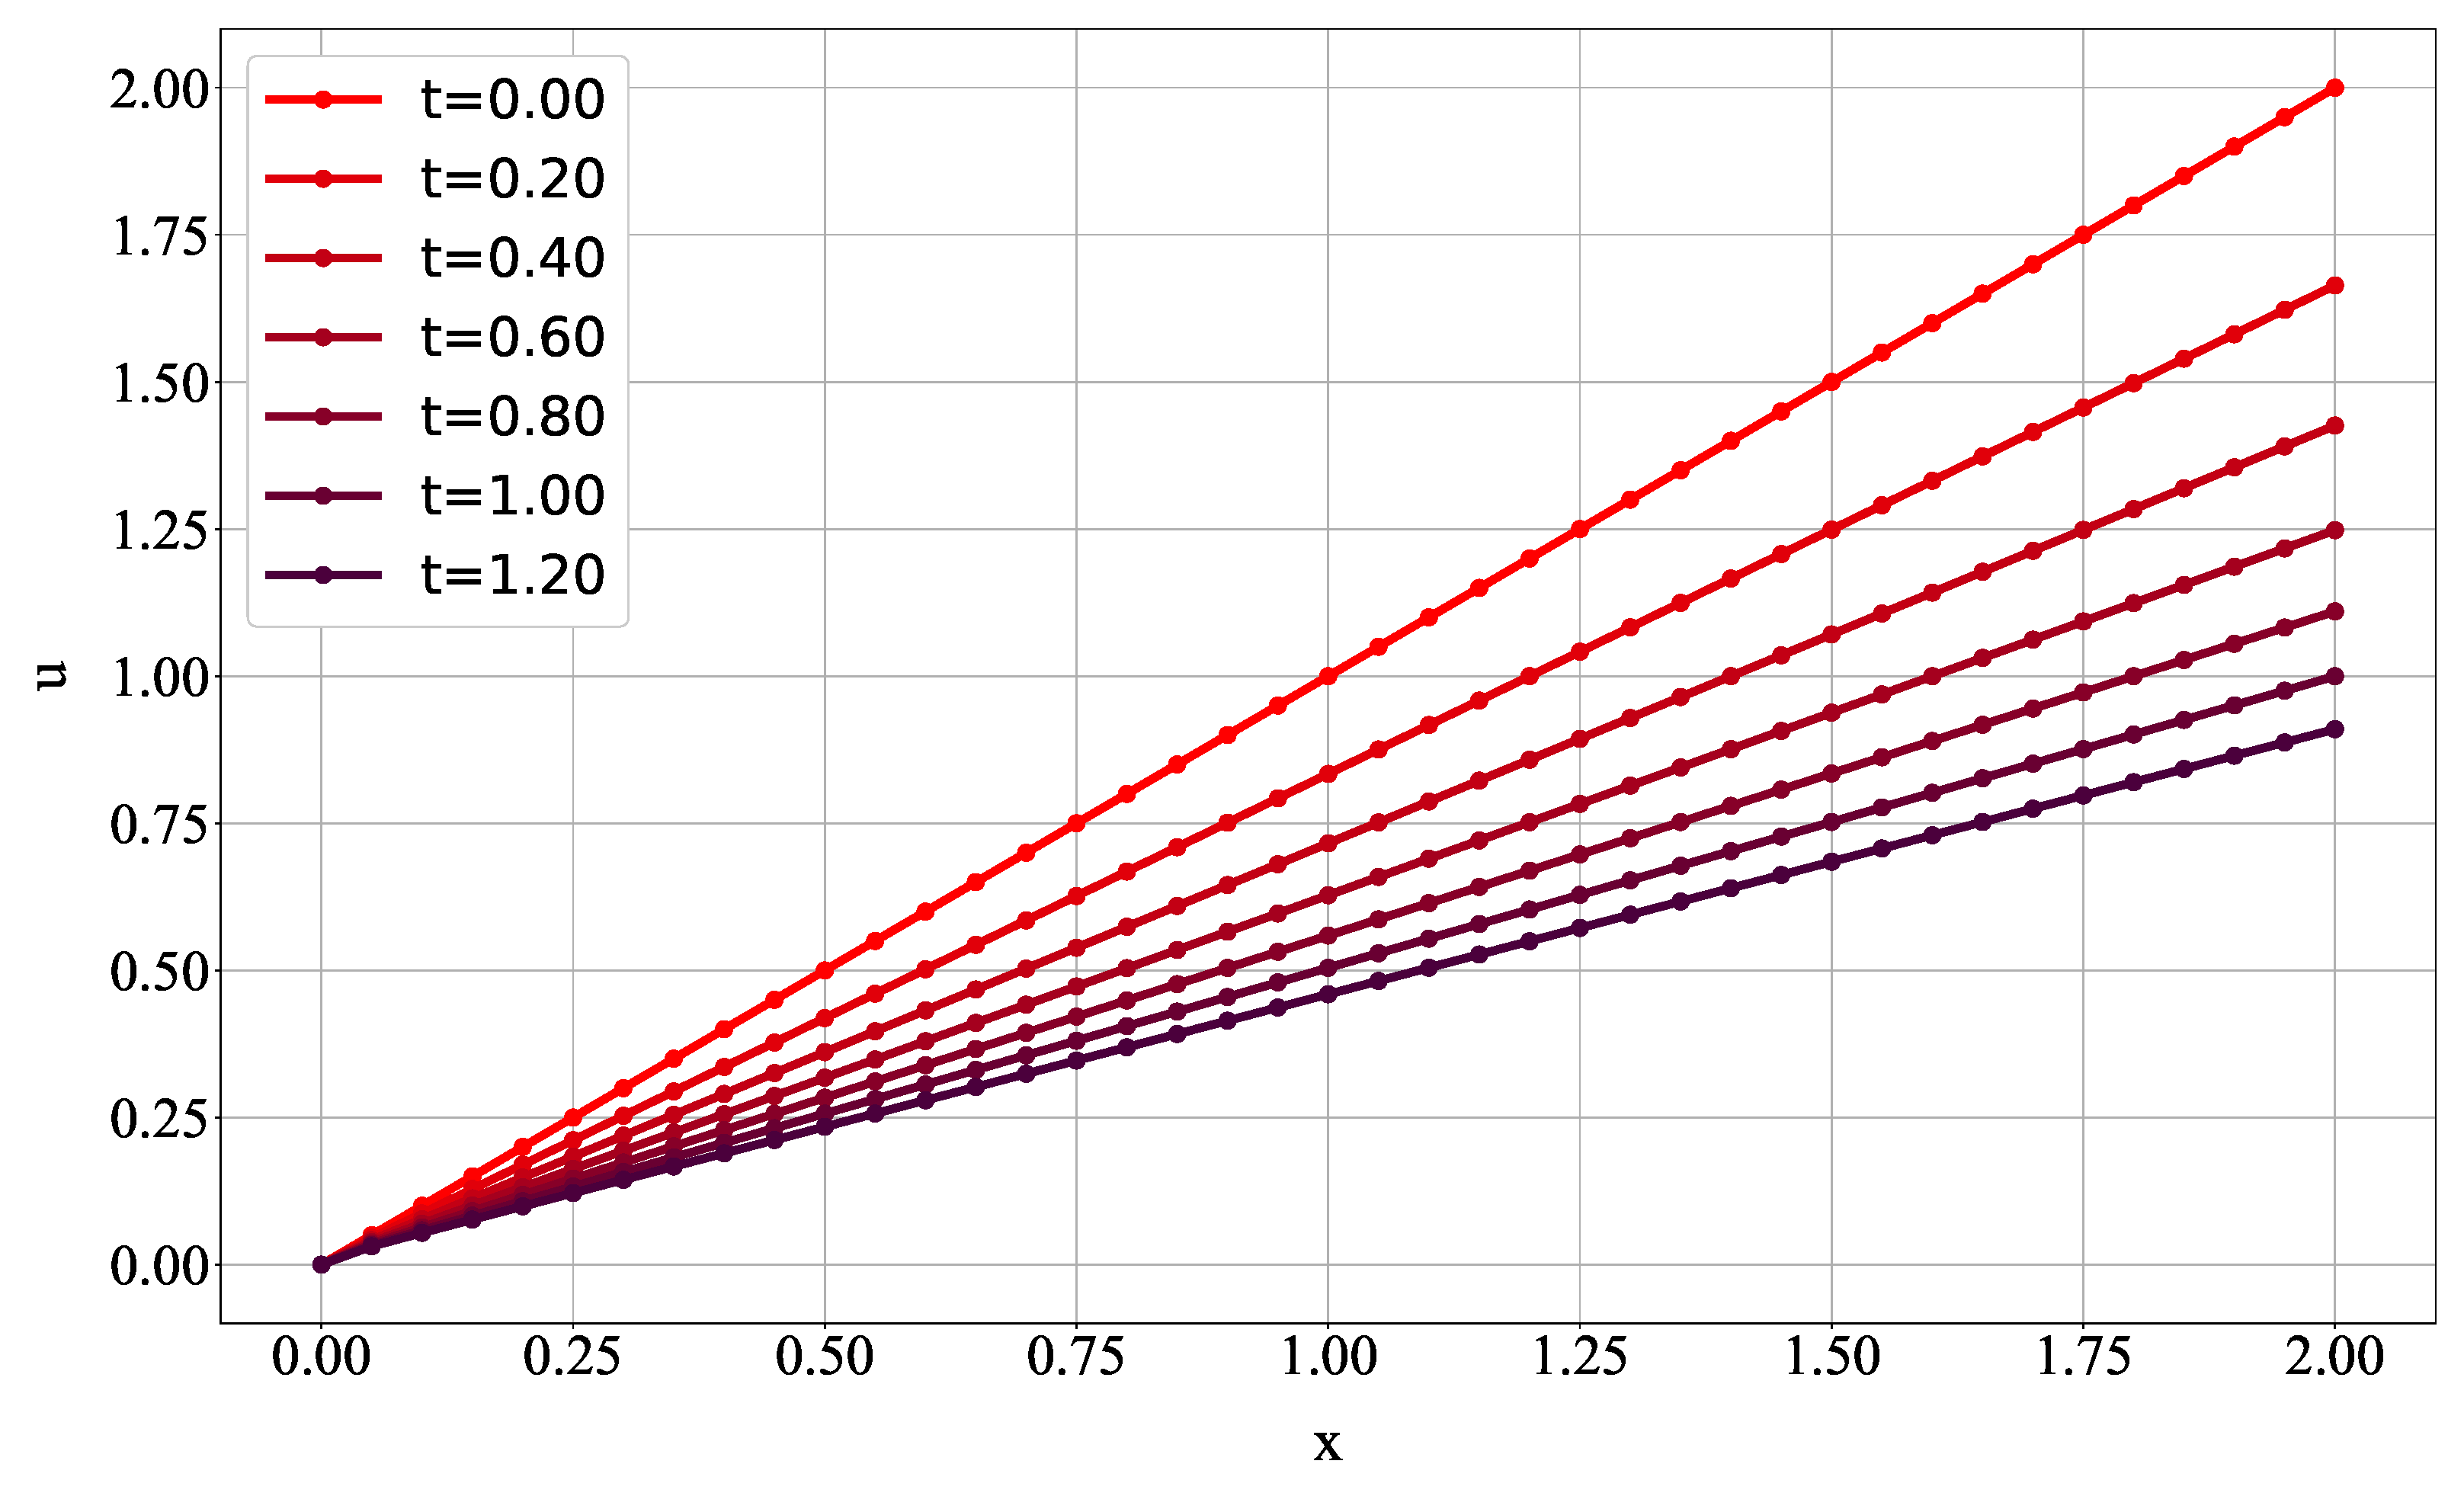
\includegraphics[width=0.425\linewidth]{3.cir.cour05.f2050}} &
        \raisebox{-0.5\totalheight}{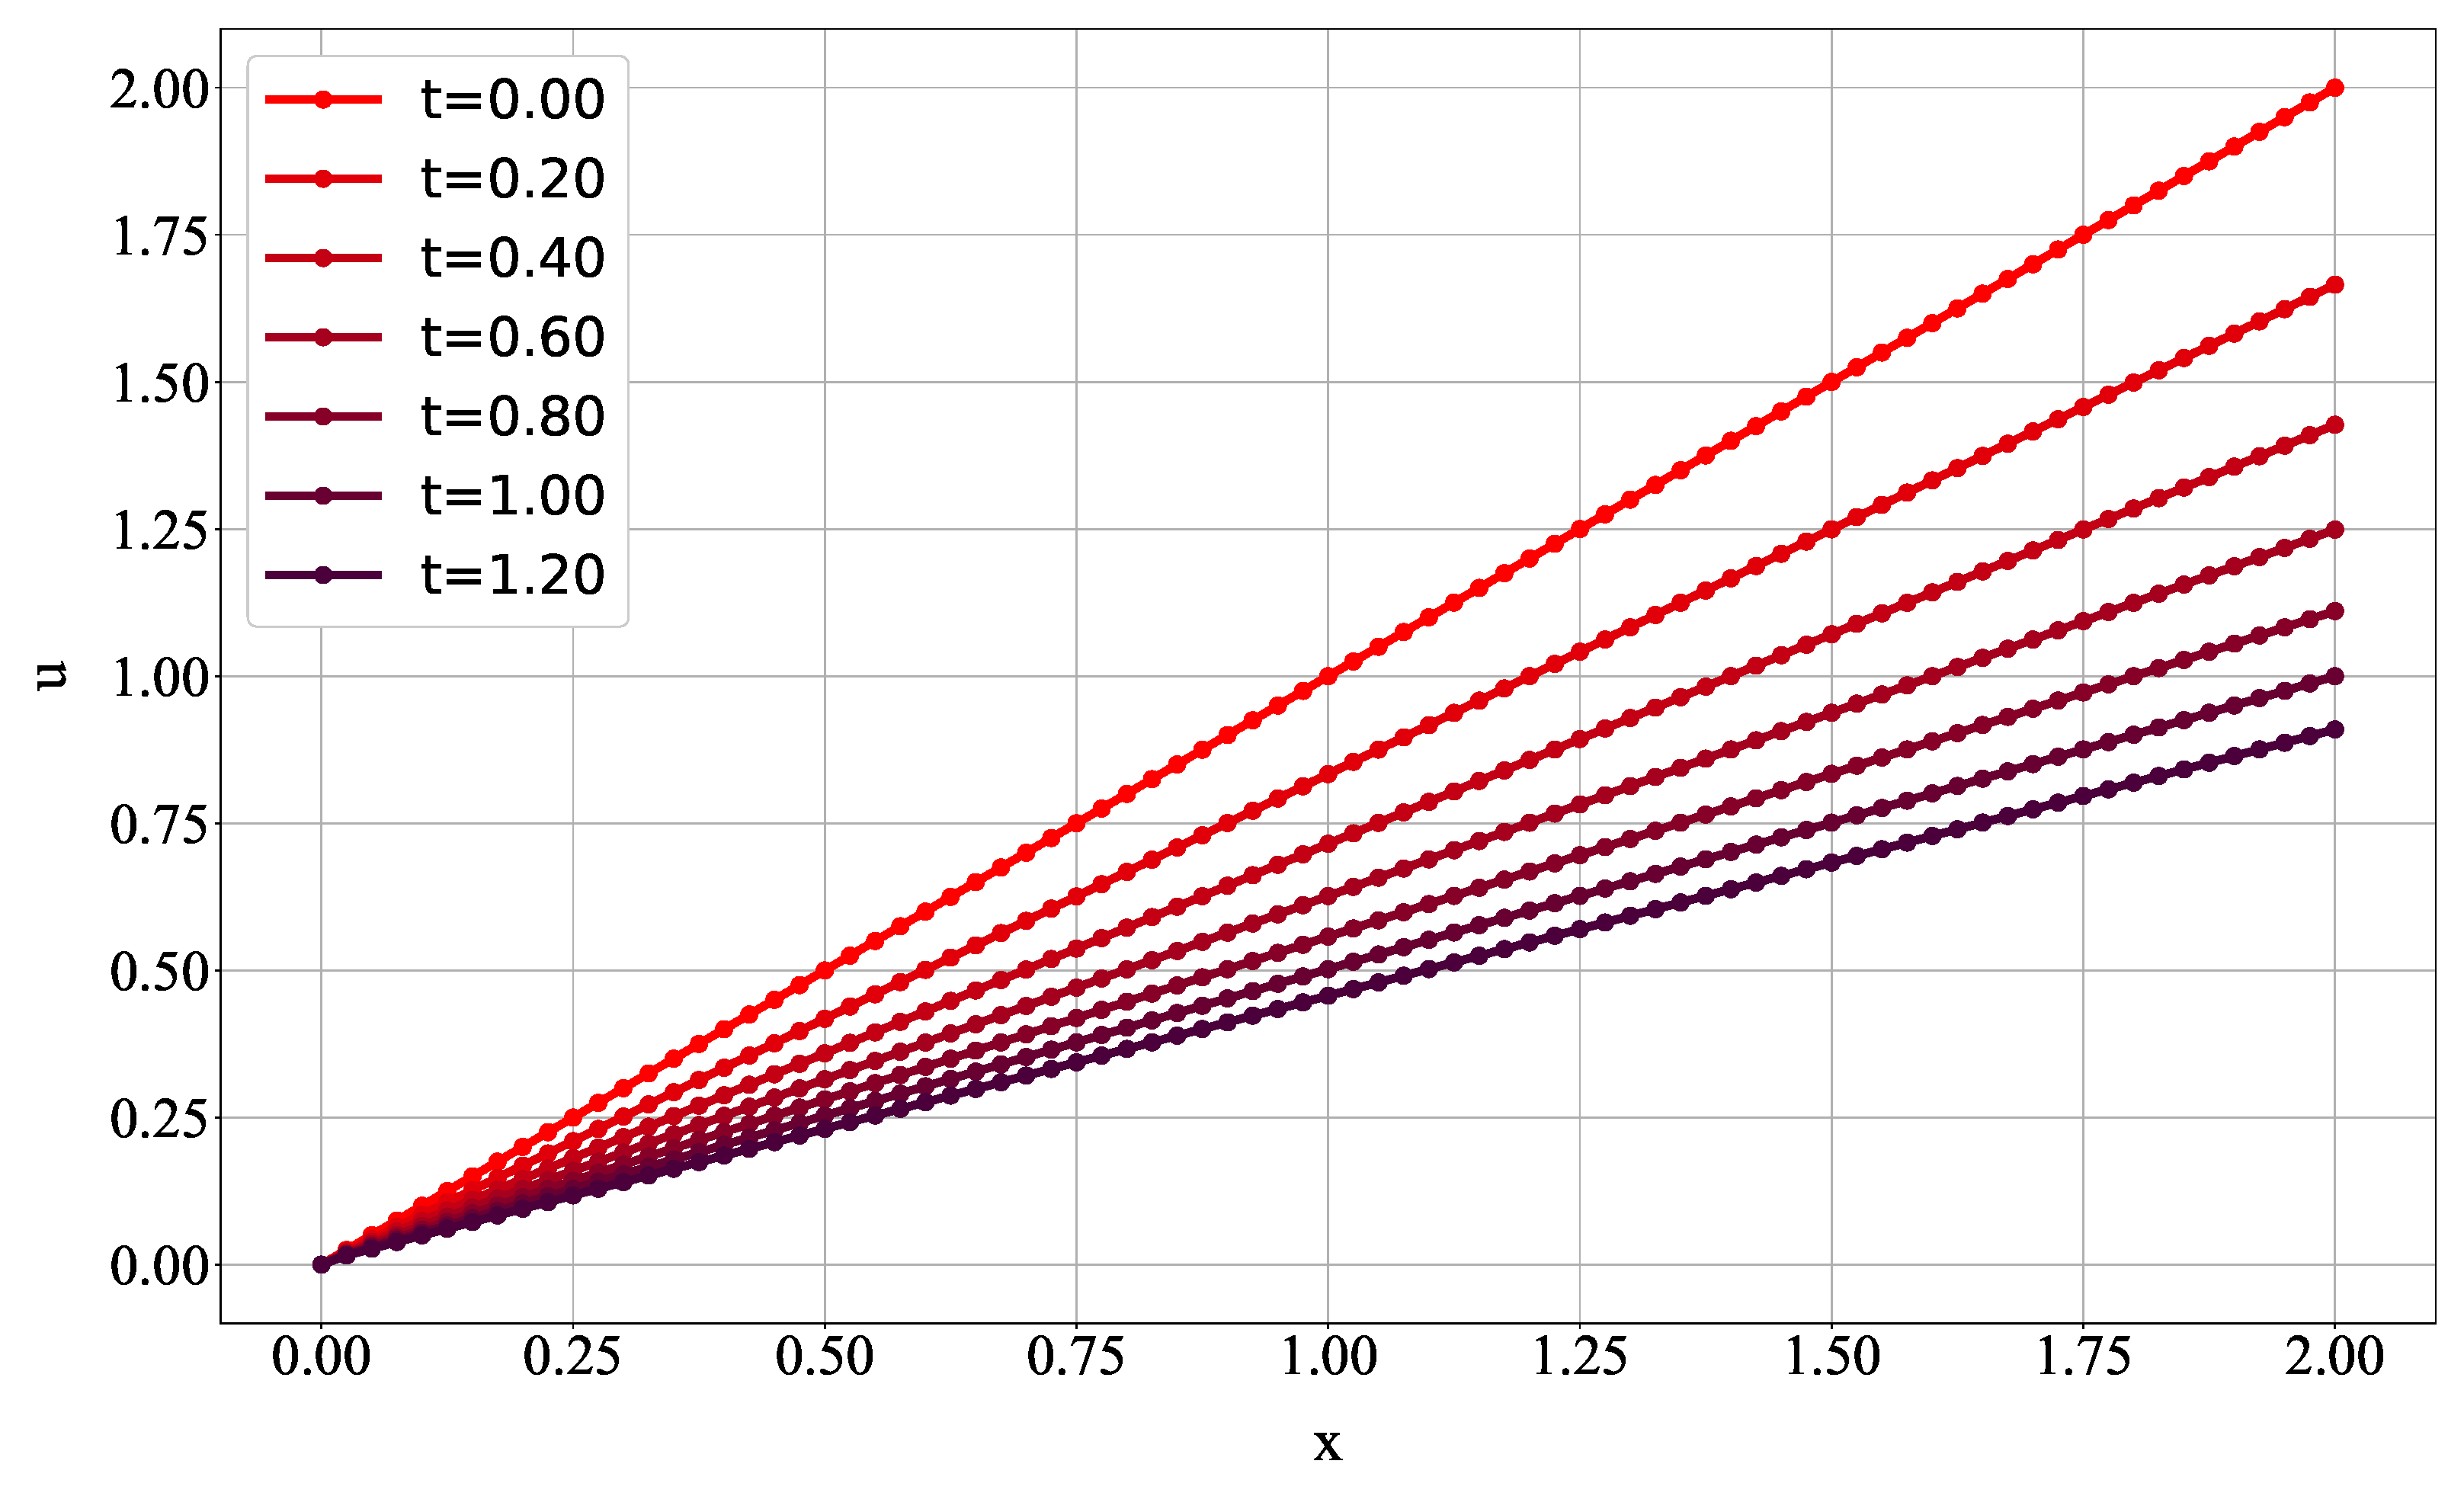
\includegraphics[width=0.425\linewidth]{3.cir.cour05.f2025}}\\
      %\cmidrule{3-4}
      {}                                          & $0.9$    &
        \raisebox{-0.5\totalheight}{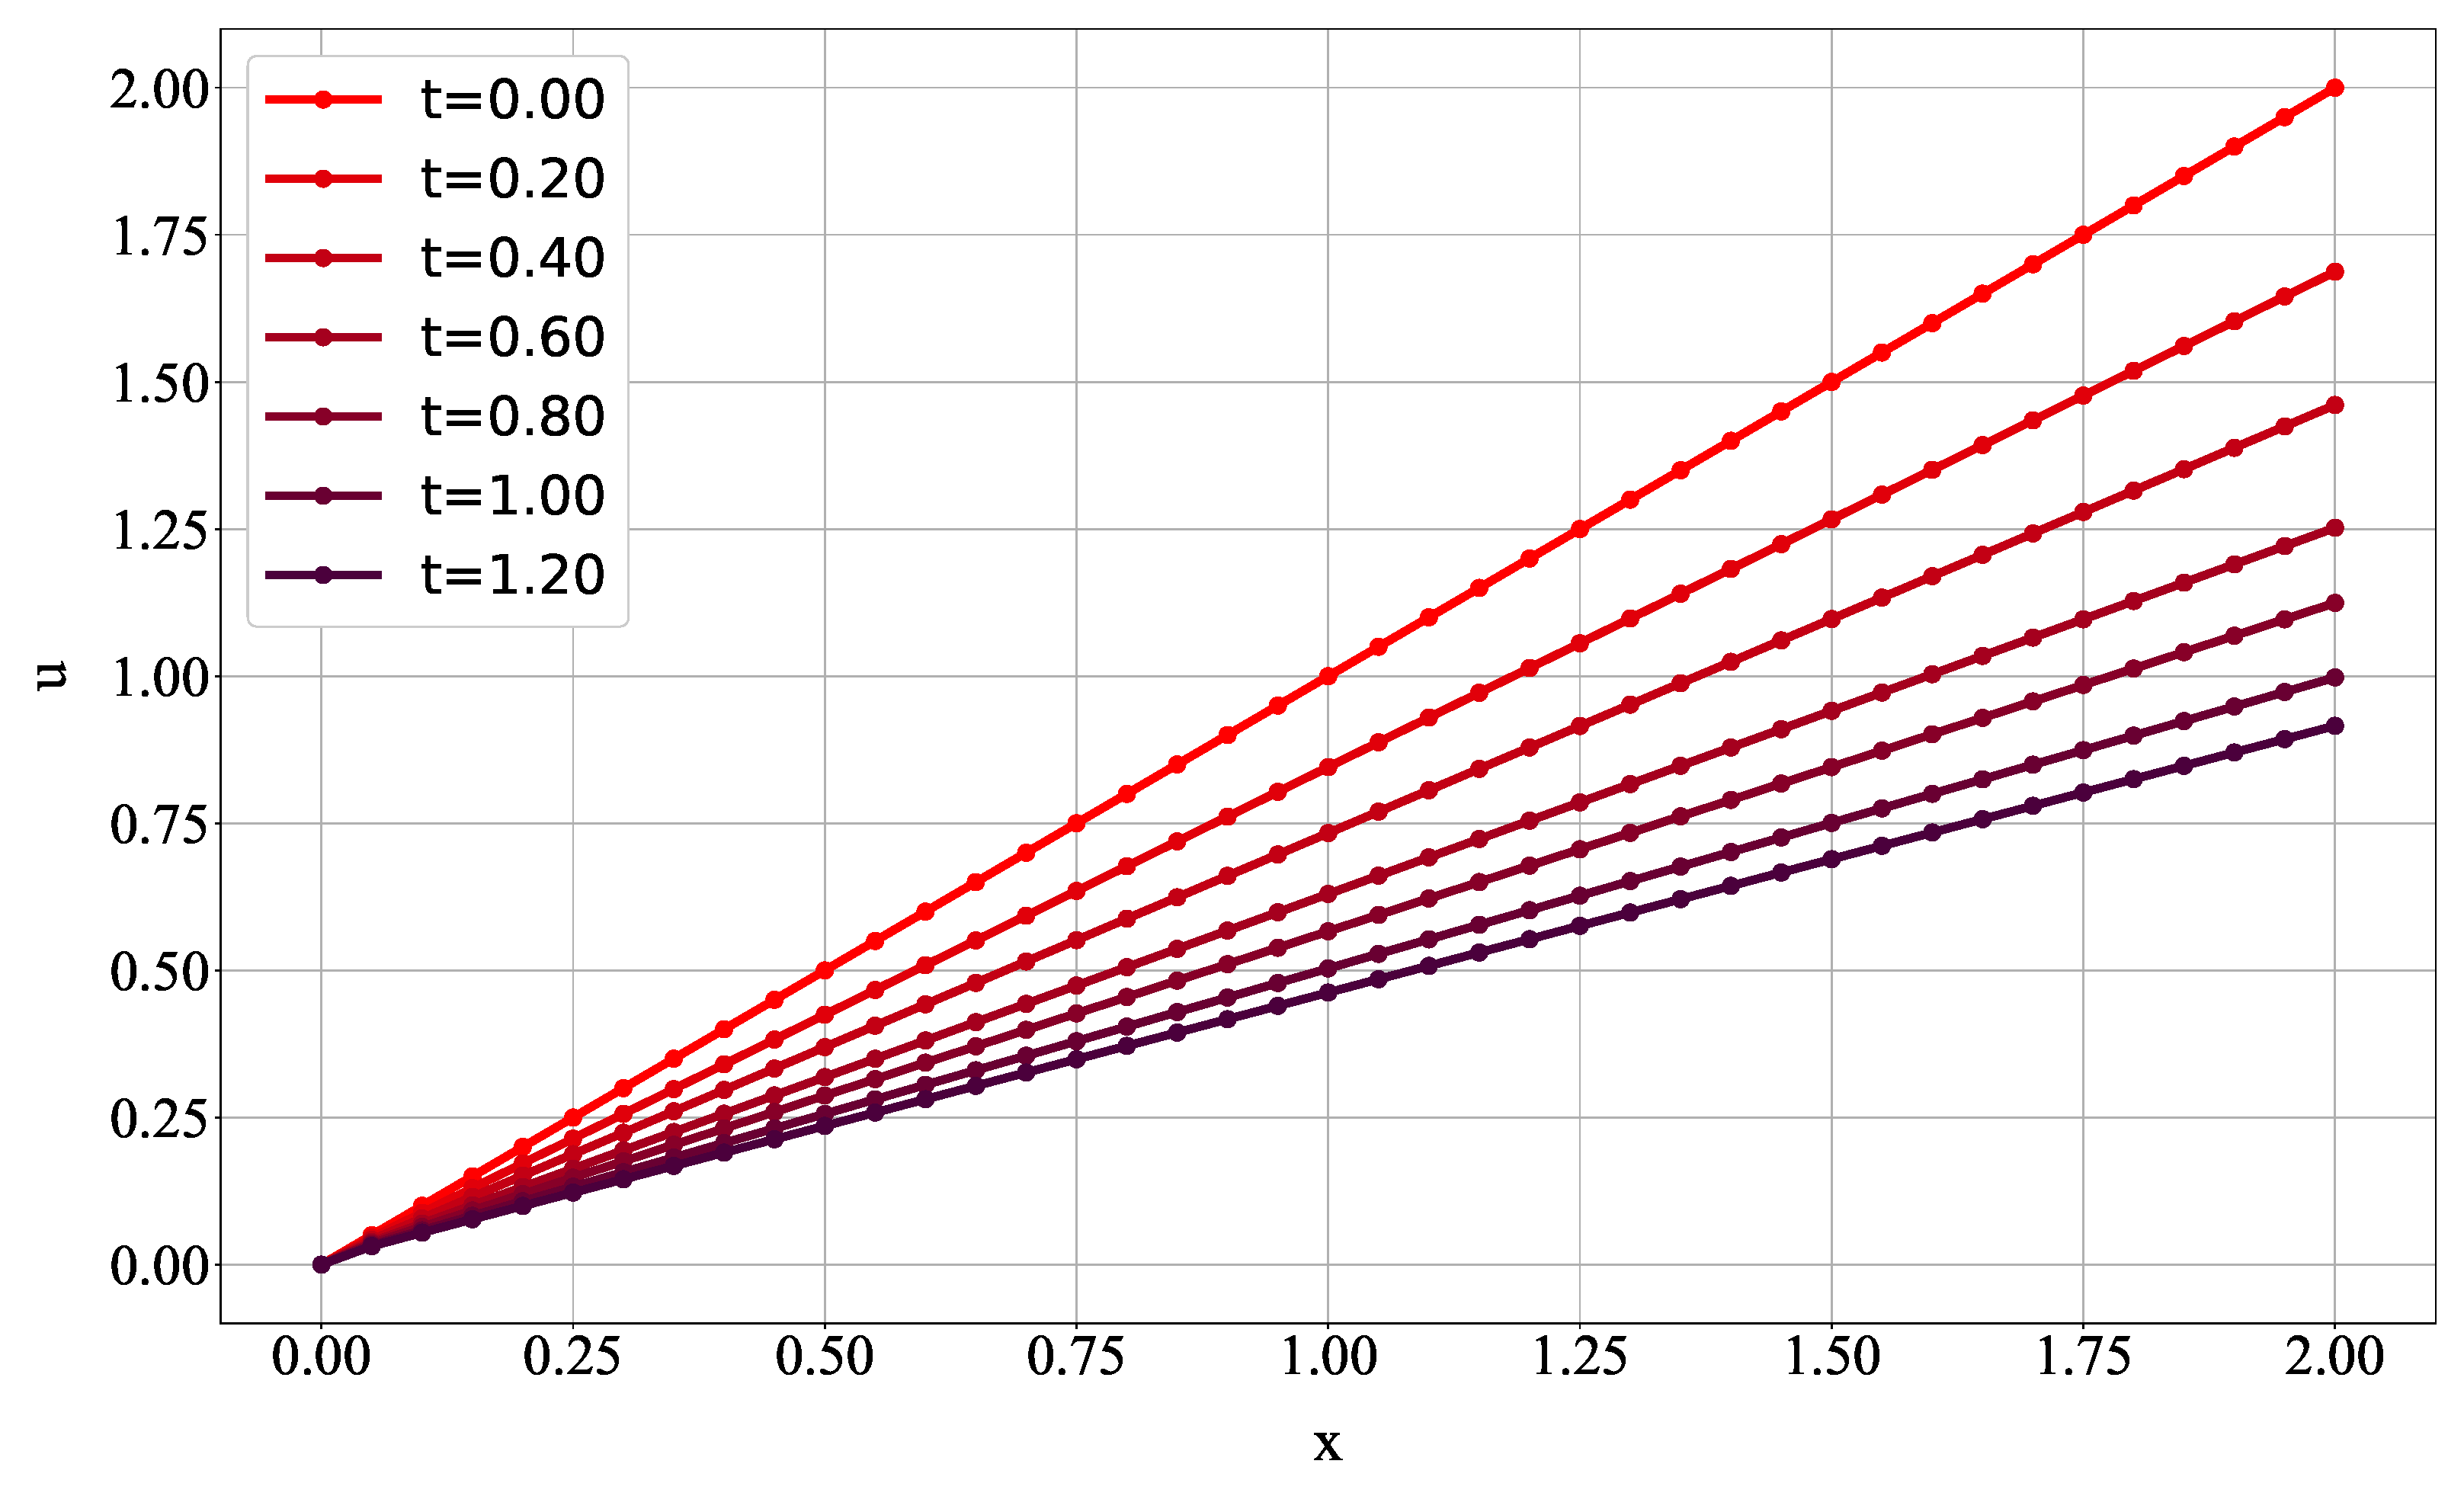
\includegraphics[width=0.425\linewidth]{3.cir.cour09.f2050}} &
        \raisebox{-0.5\totalheight}{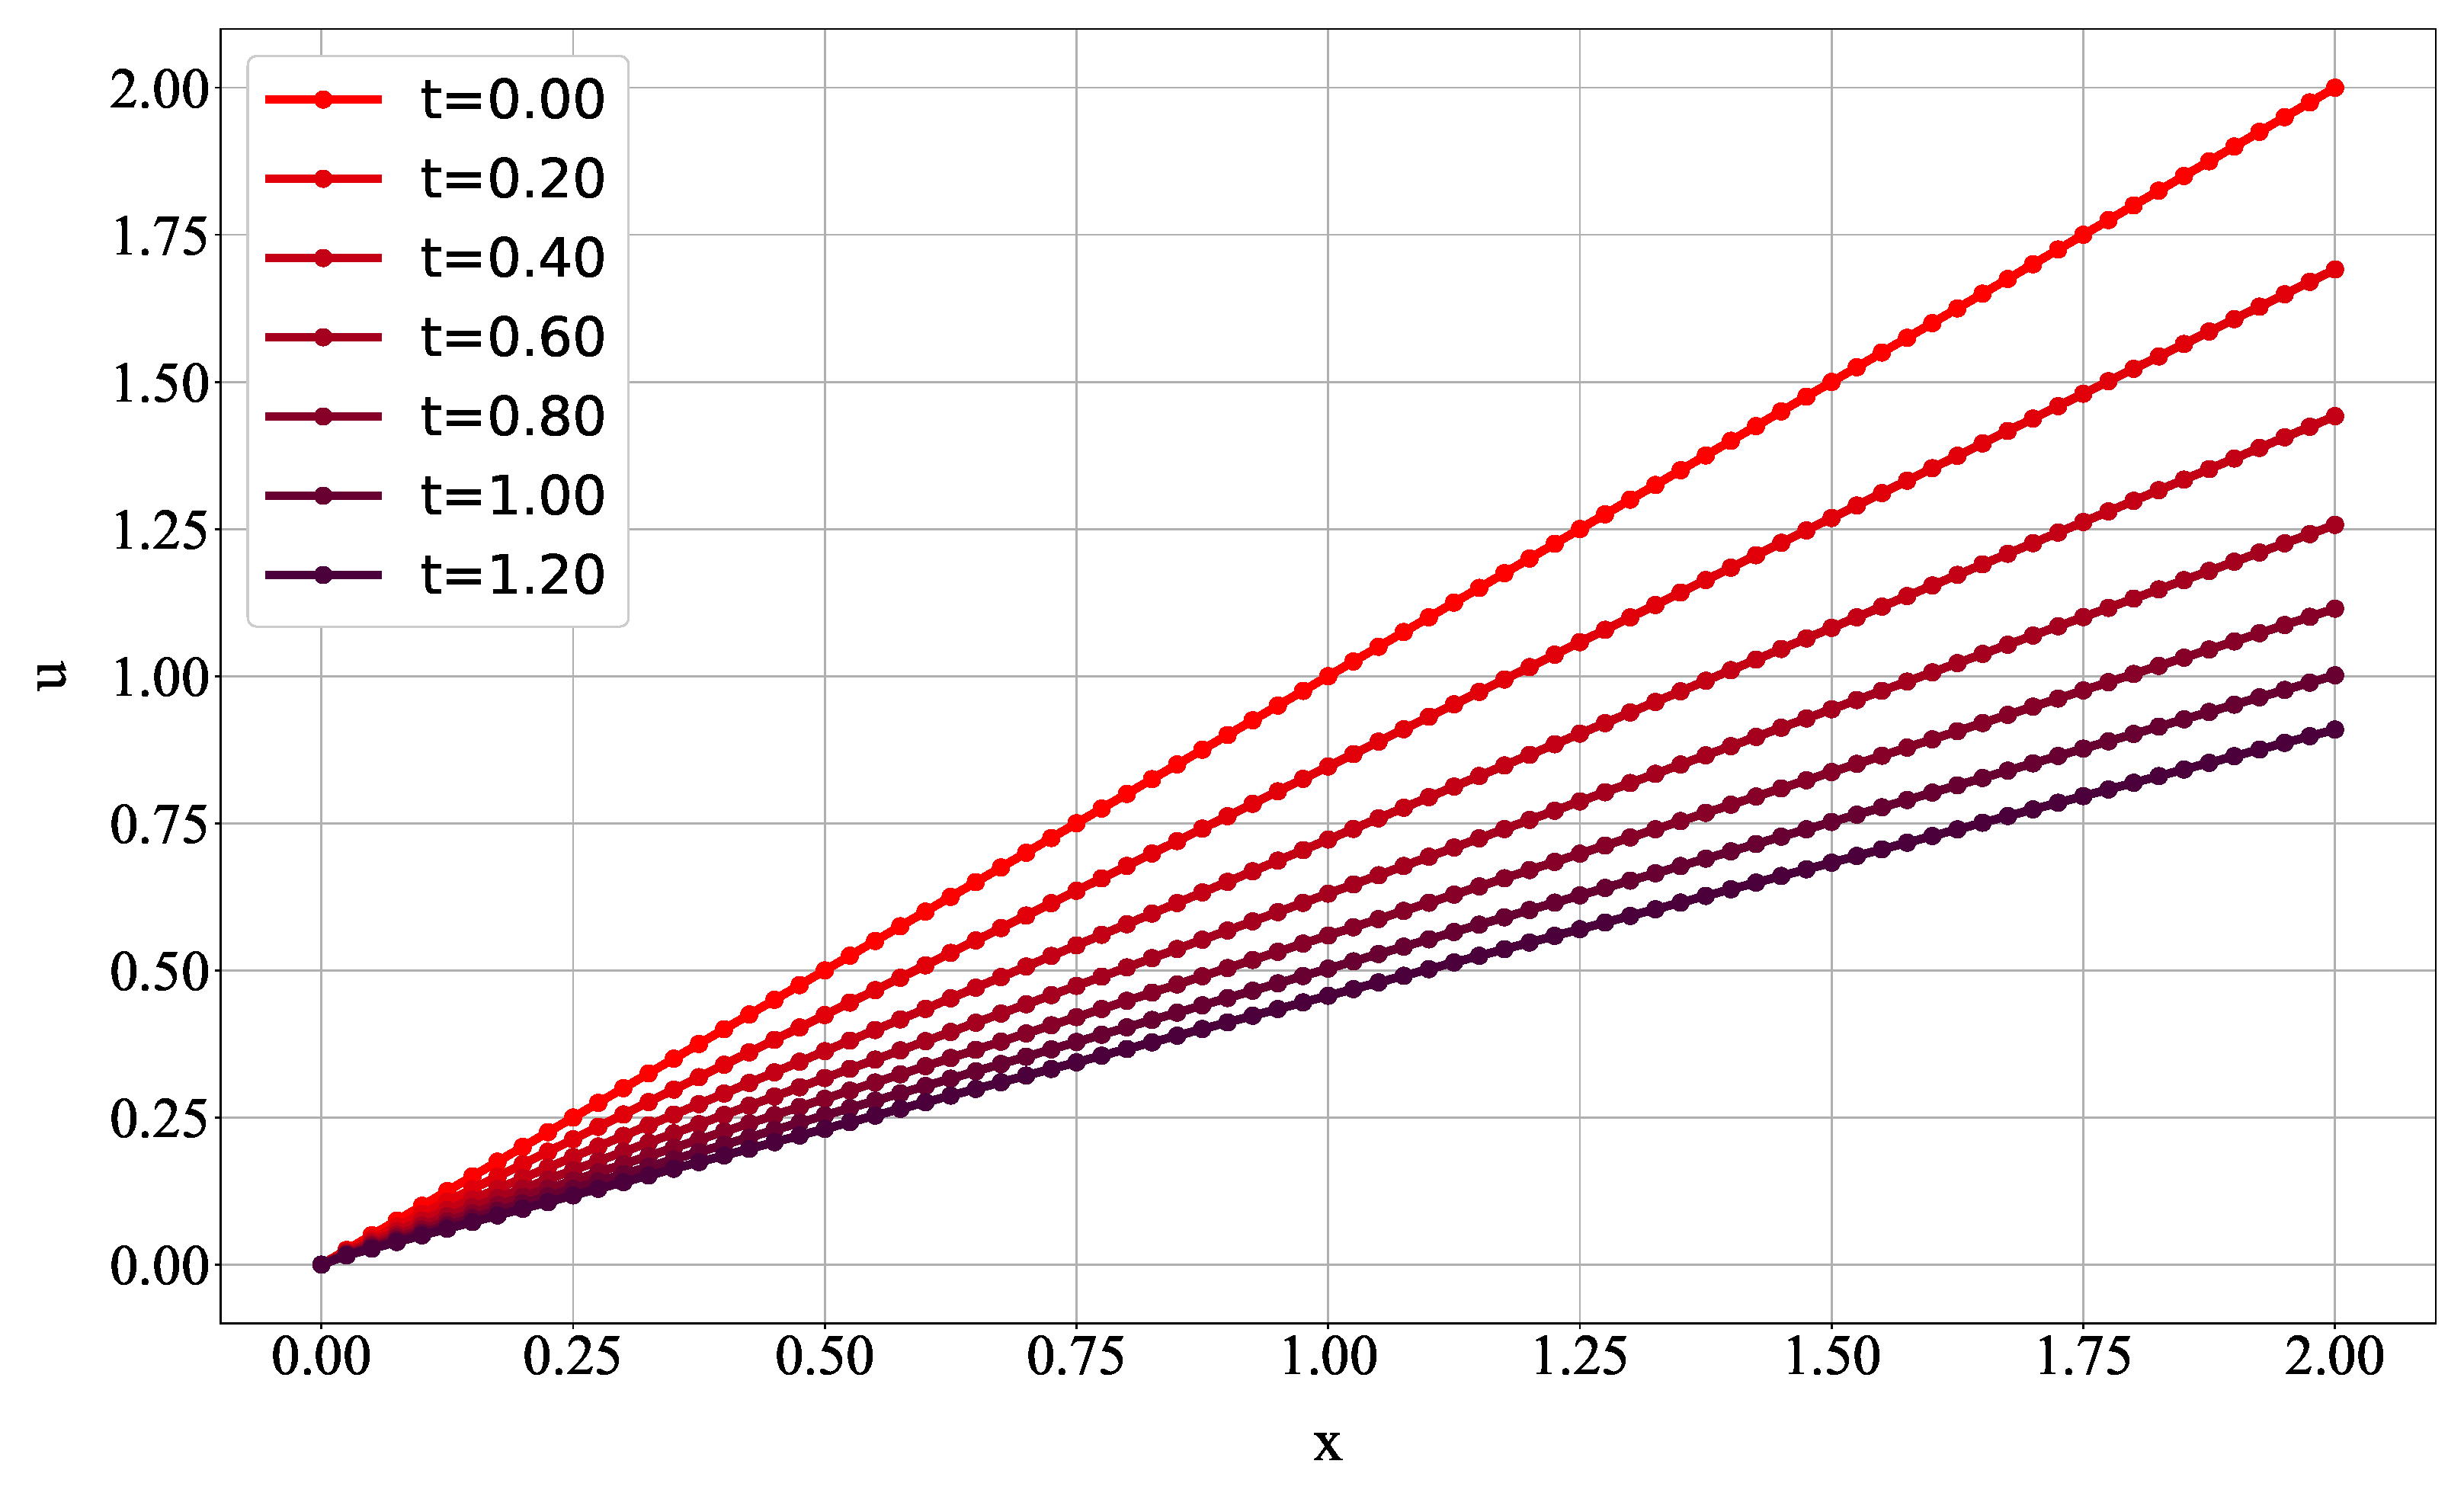
\includegraphics[width=0.425\linewidth]{3.cir.cour09.f2025}}\\
      \bottomrule
    \end{tabular}
  \end{center}
  \end{table}

  \begin{table}[p]
  \caption{"`Лакс-Вендрофф"' (\ref{sec:lax-vendroff})}
  \label{plot:lax-vendroff}
  \begin{center}
    \begin{tabular}{c c c c}
      \toprule
      {$f$}                                       & $\sigma$ & $h_1$ & $h_2$\\
      \midrule
      \multirow{2}{*}{\vspace{\myvspaceOne}$f_1$} & $0.5$    & 
        \raisebox{-0.5\totalheight}{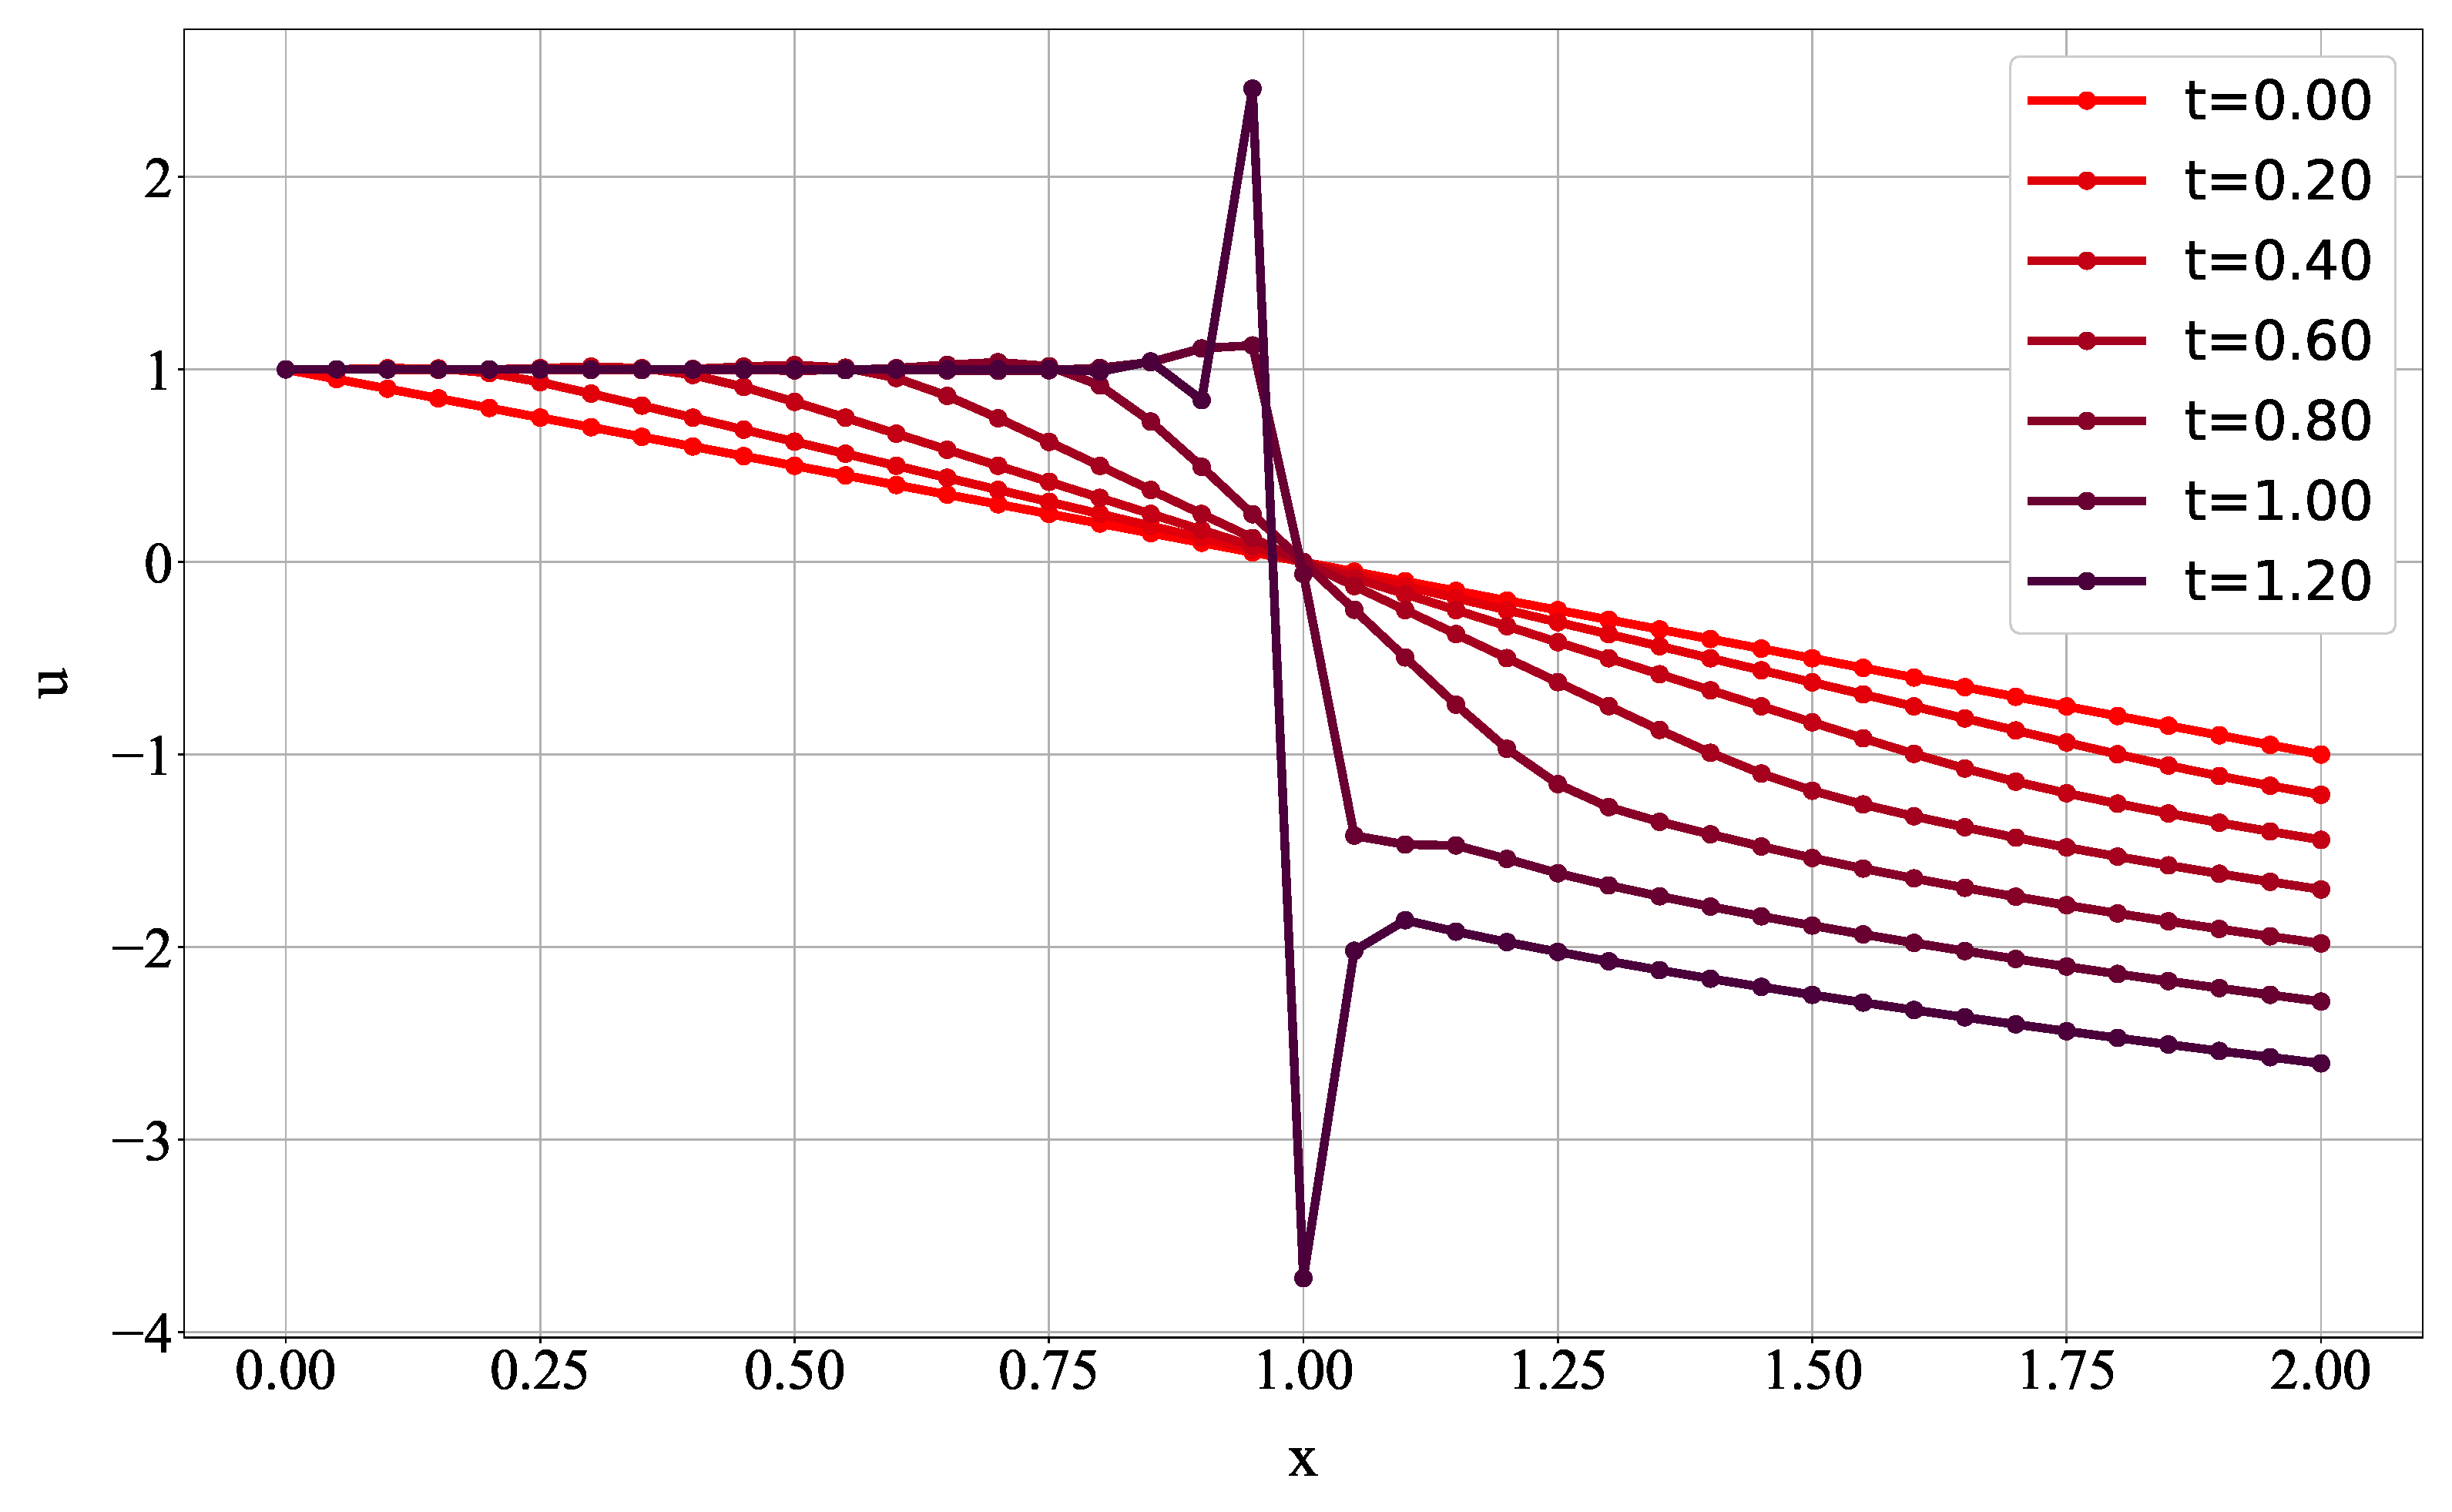
\includegraphics[width=0.425\linewidth]{4.lax-vendroff.cour05.f1050}} &
        \raisebox{-0.5\totalheight}{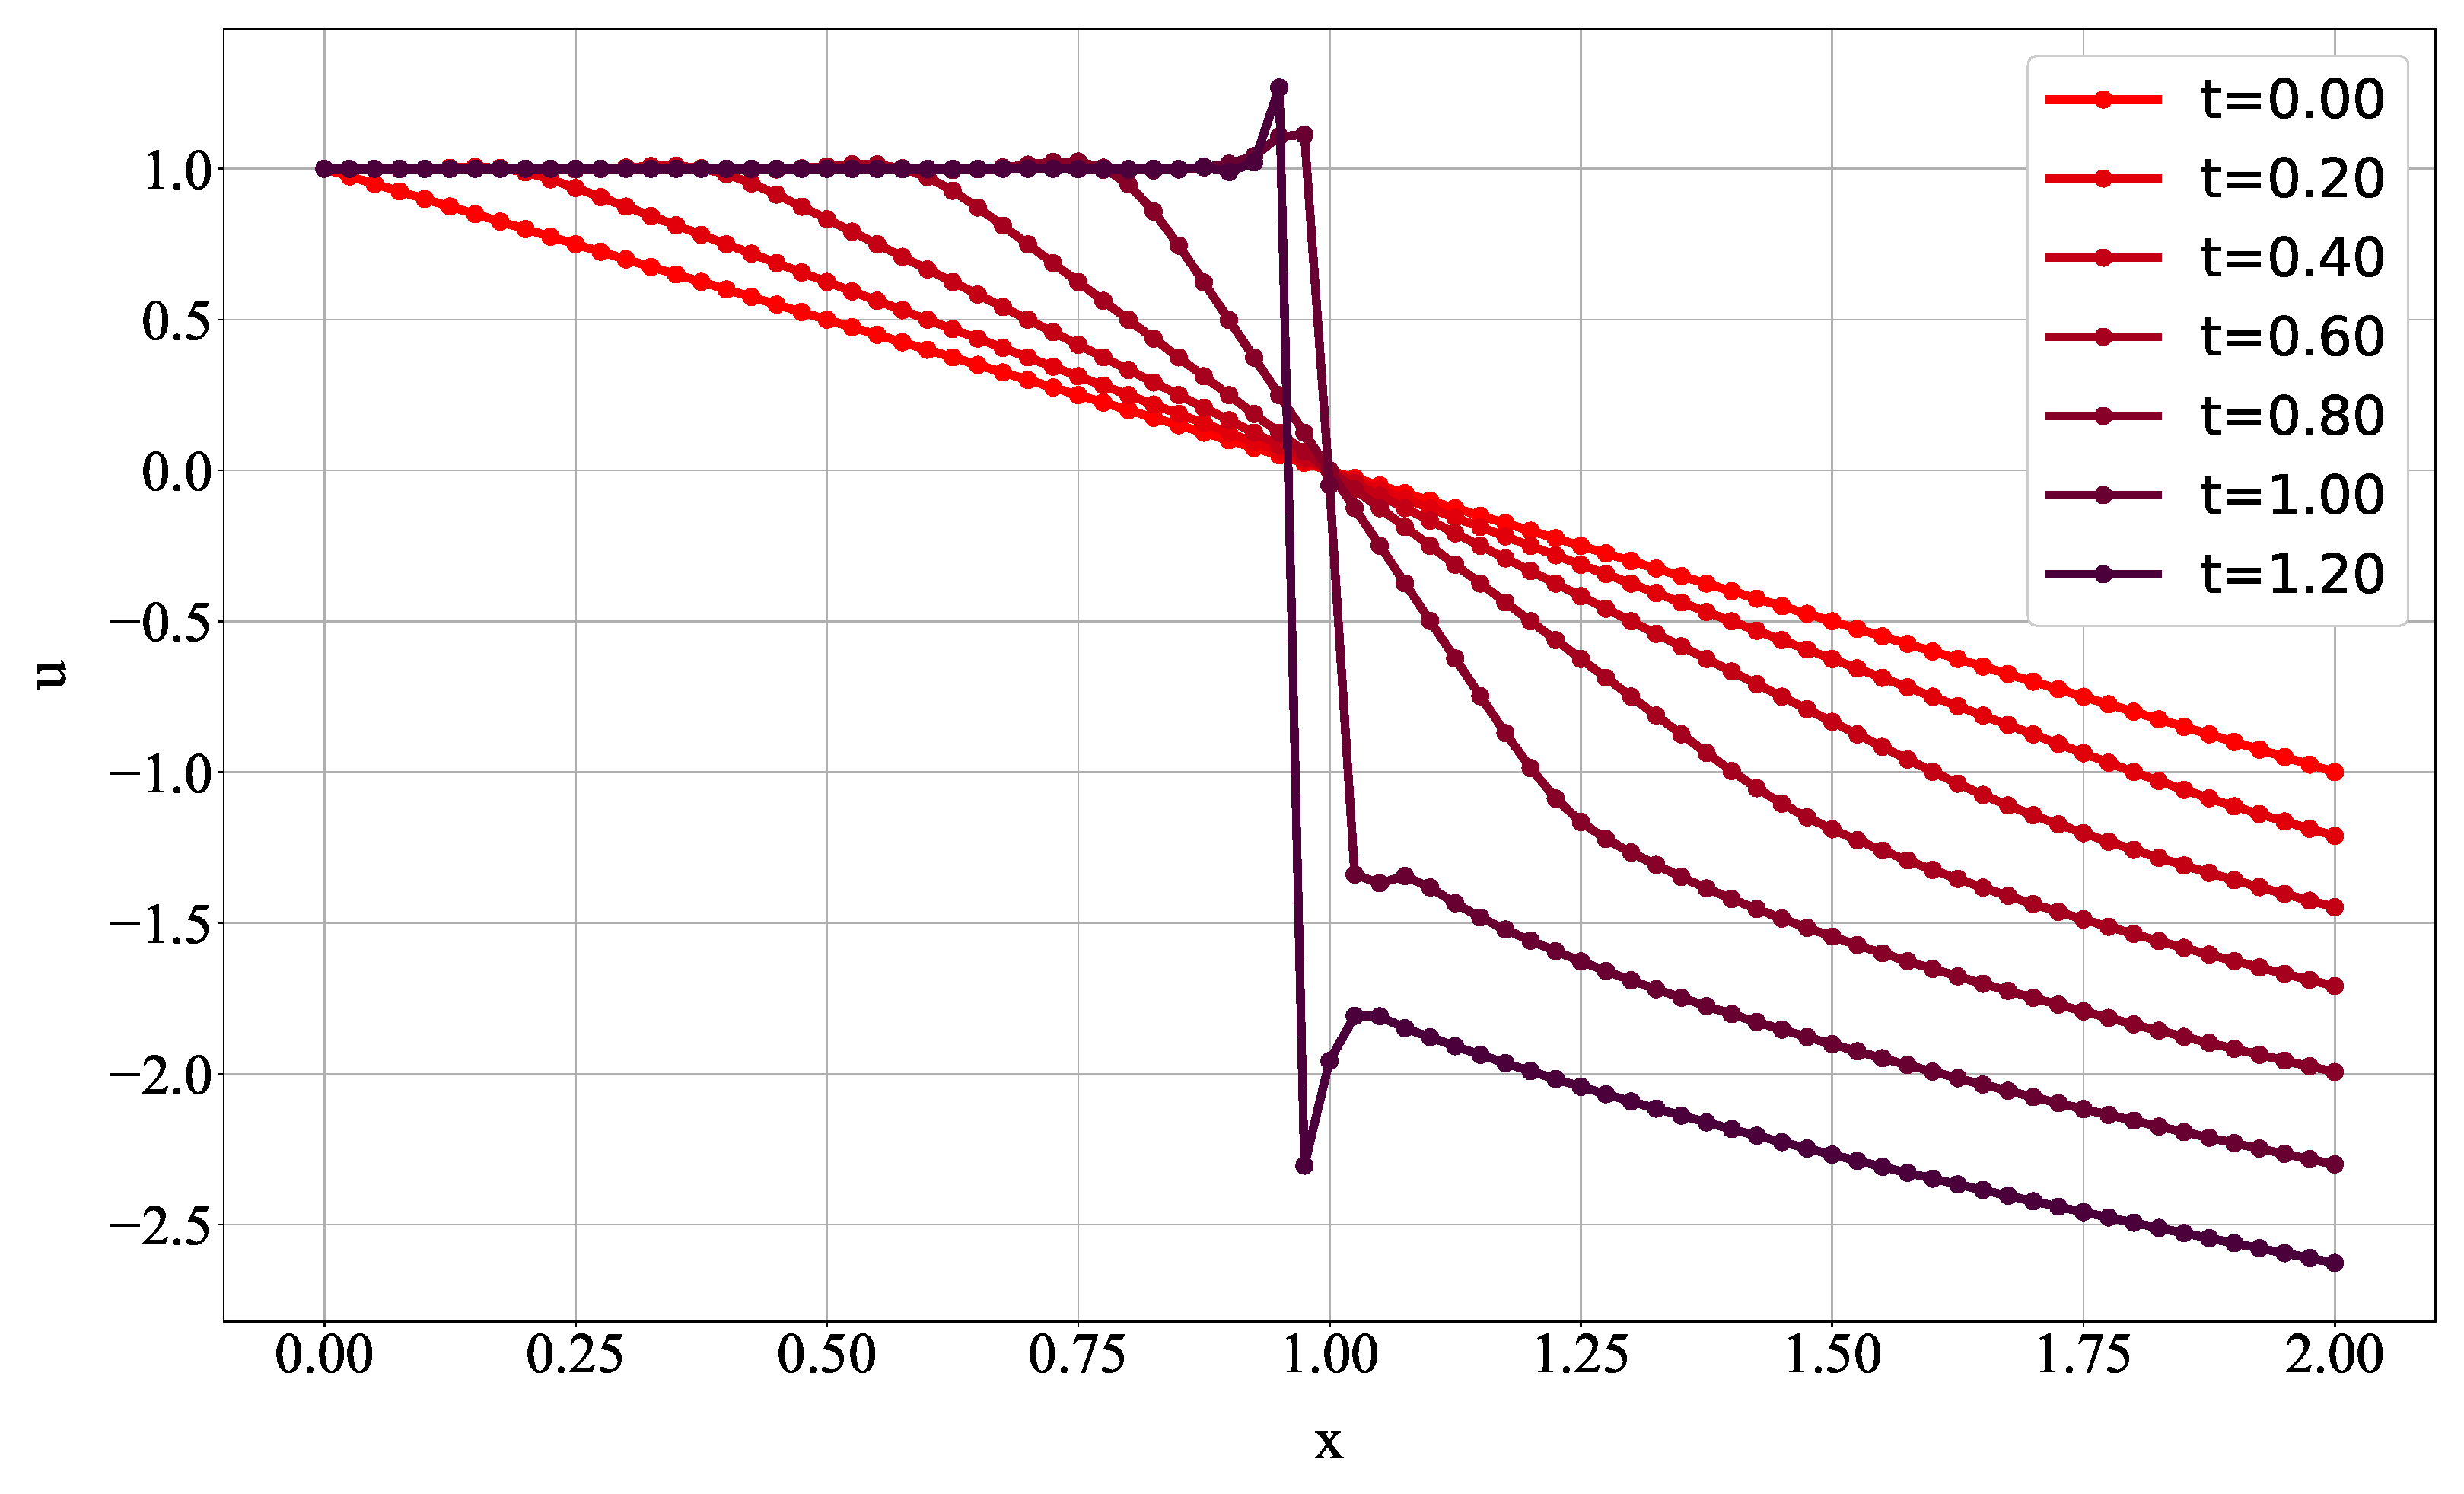
\includegraphics[width=0.425\linewidth]{4.lax-vendroff.cour05.f1025}}\\
      %\cmidrule{3-4}
      {}                                          & $0.9$    &
        \raisebox{-0.5\totalheight}{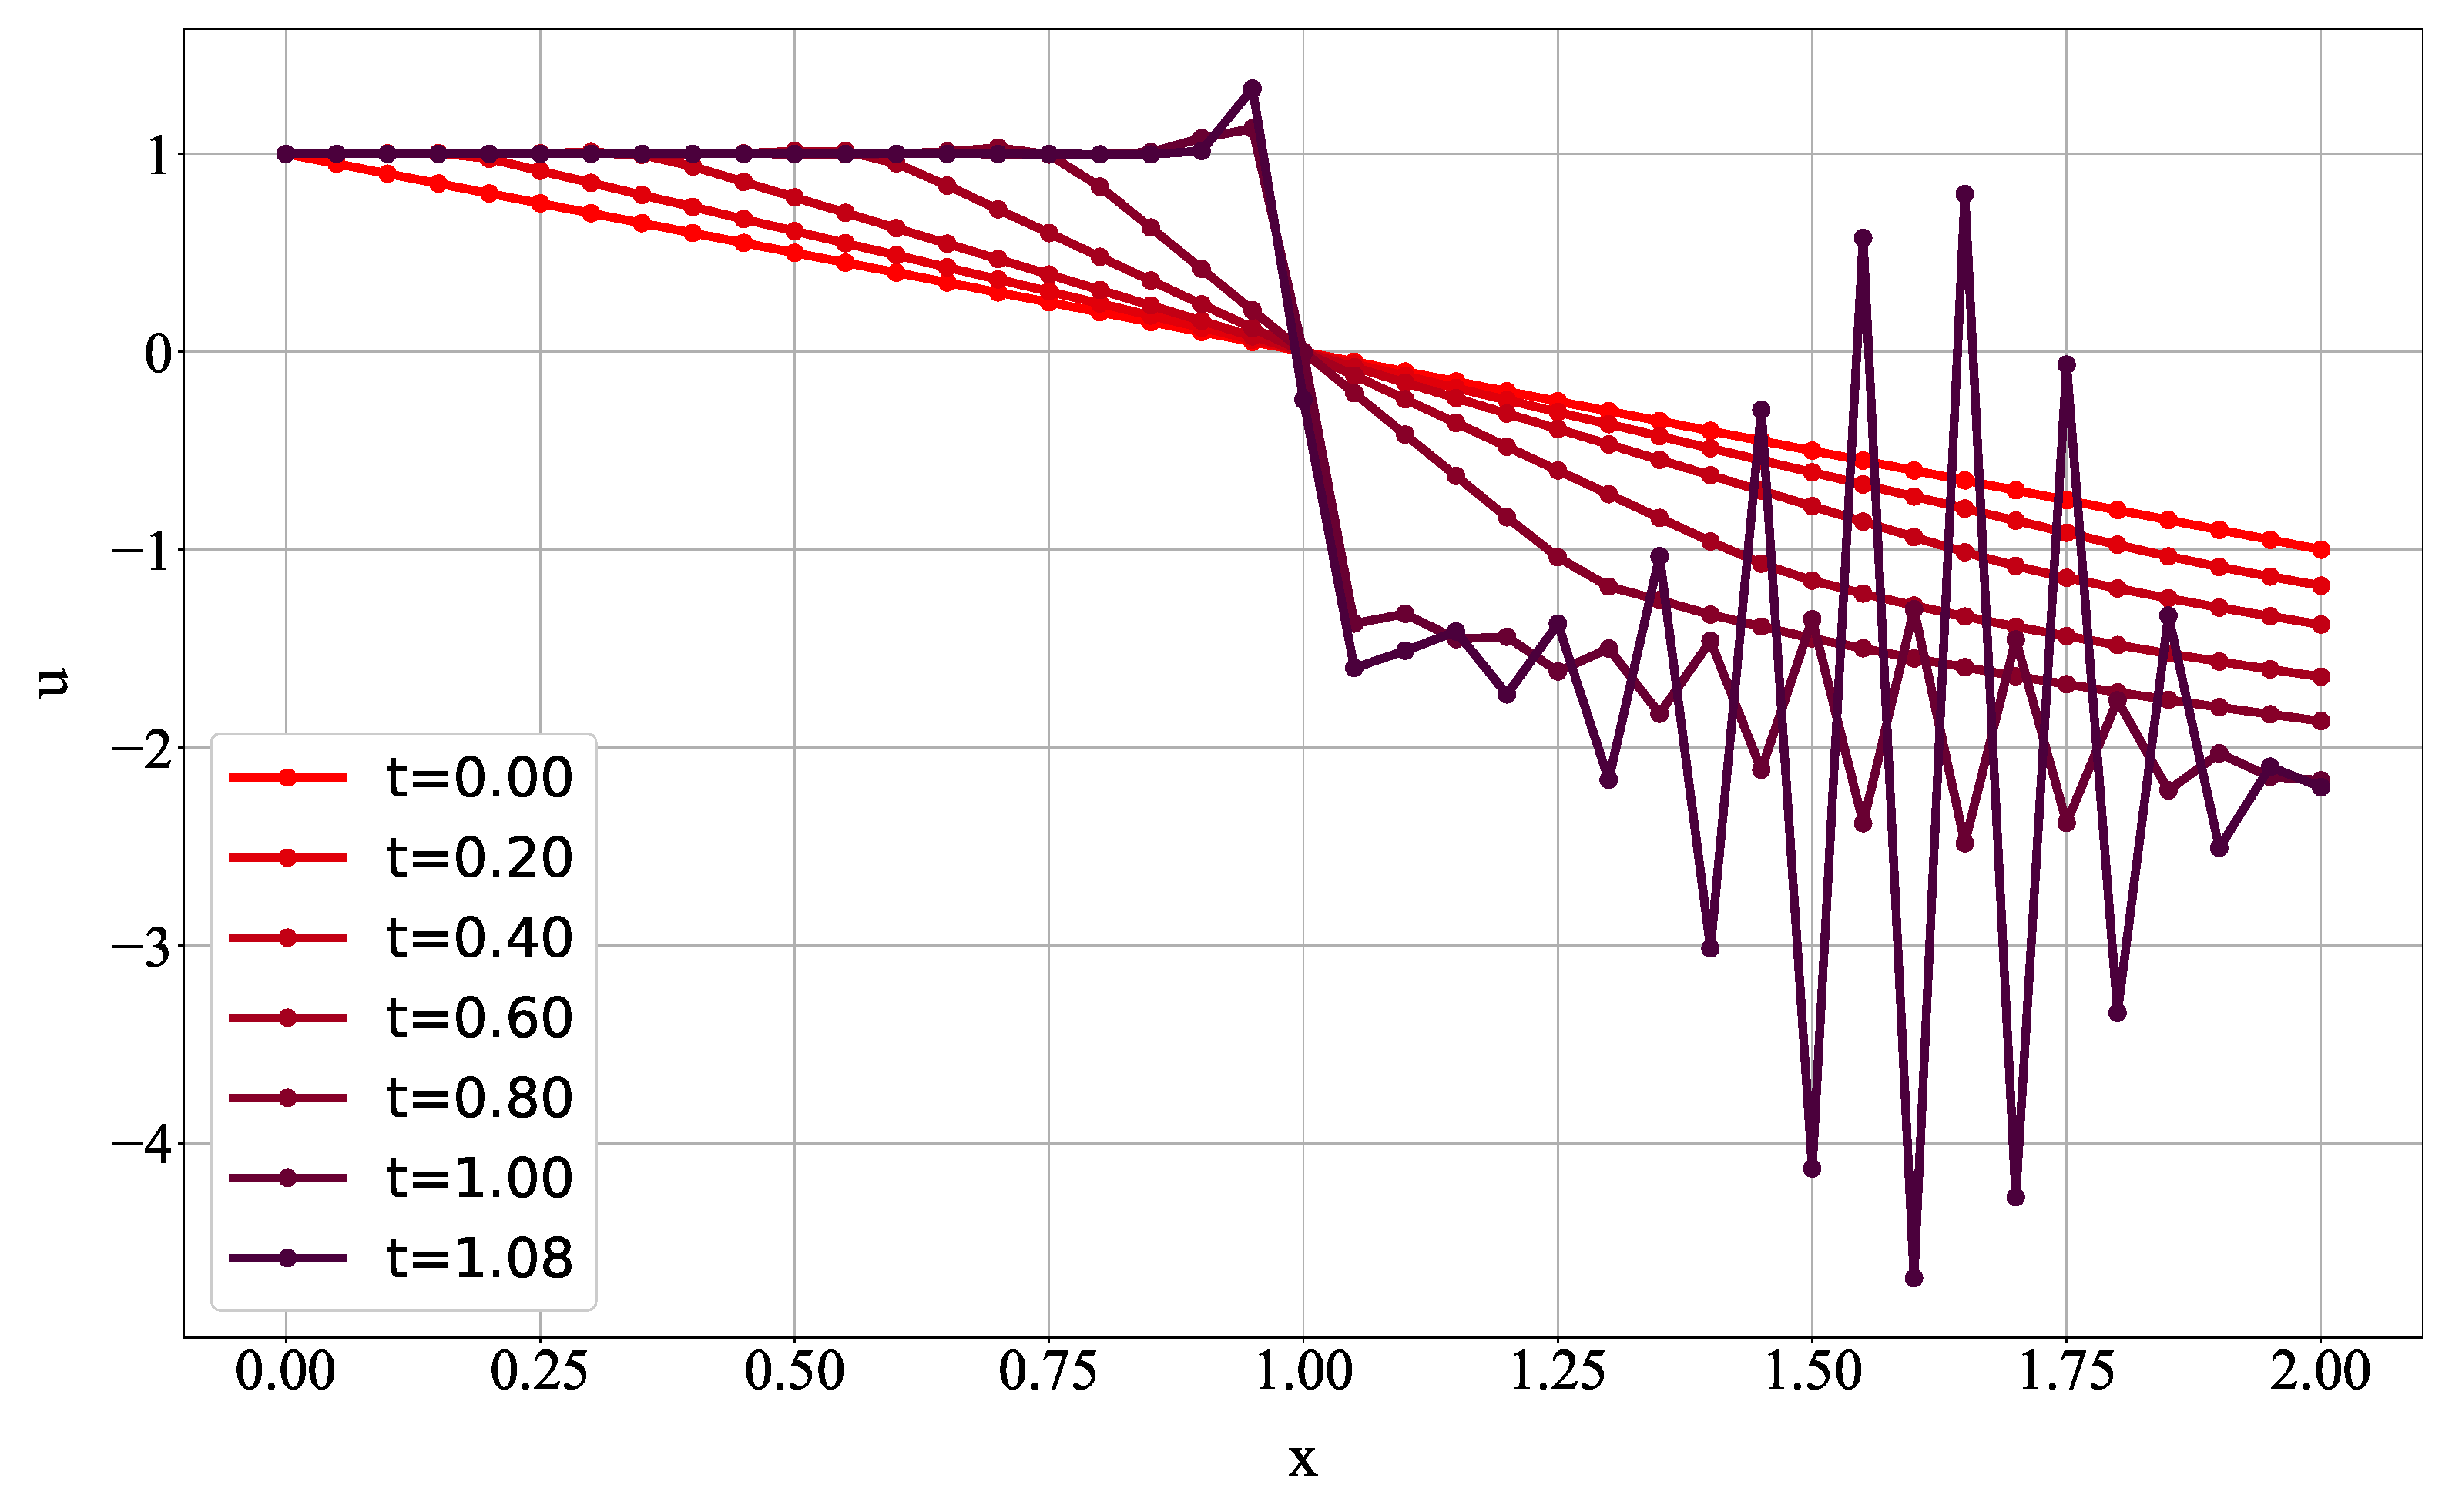
\includegraphics[width=0.425\linewidth]{4.lax-vendroff.cour09.f1050}} & 
        \raisebox{-0.5\totalheight}{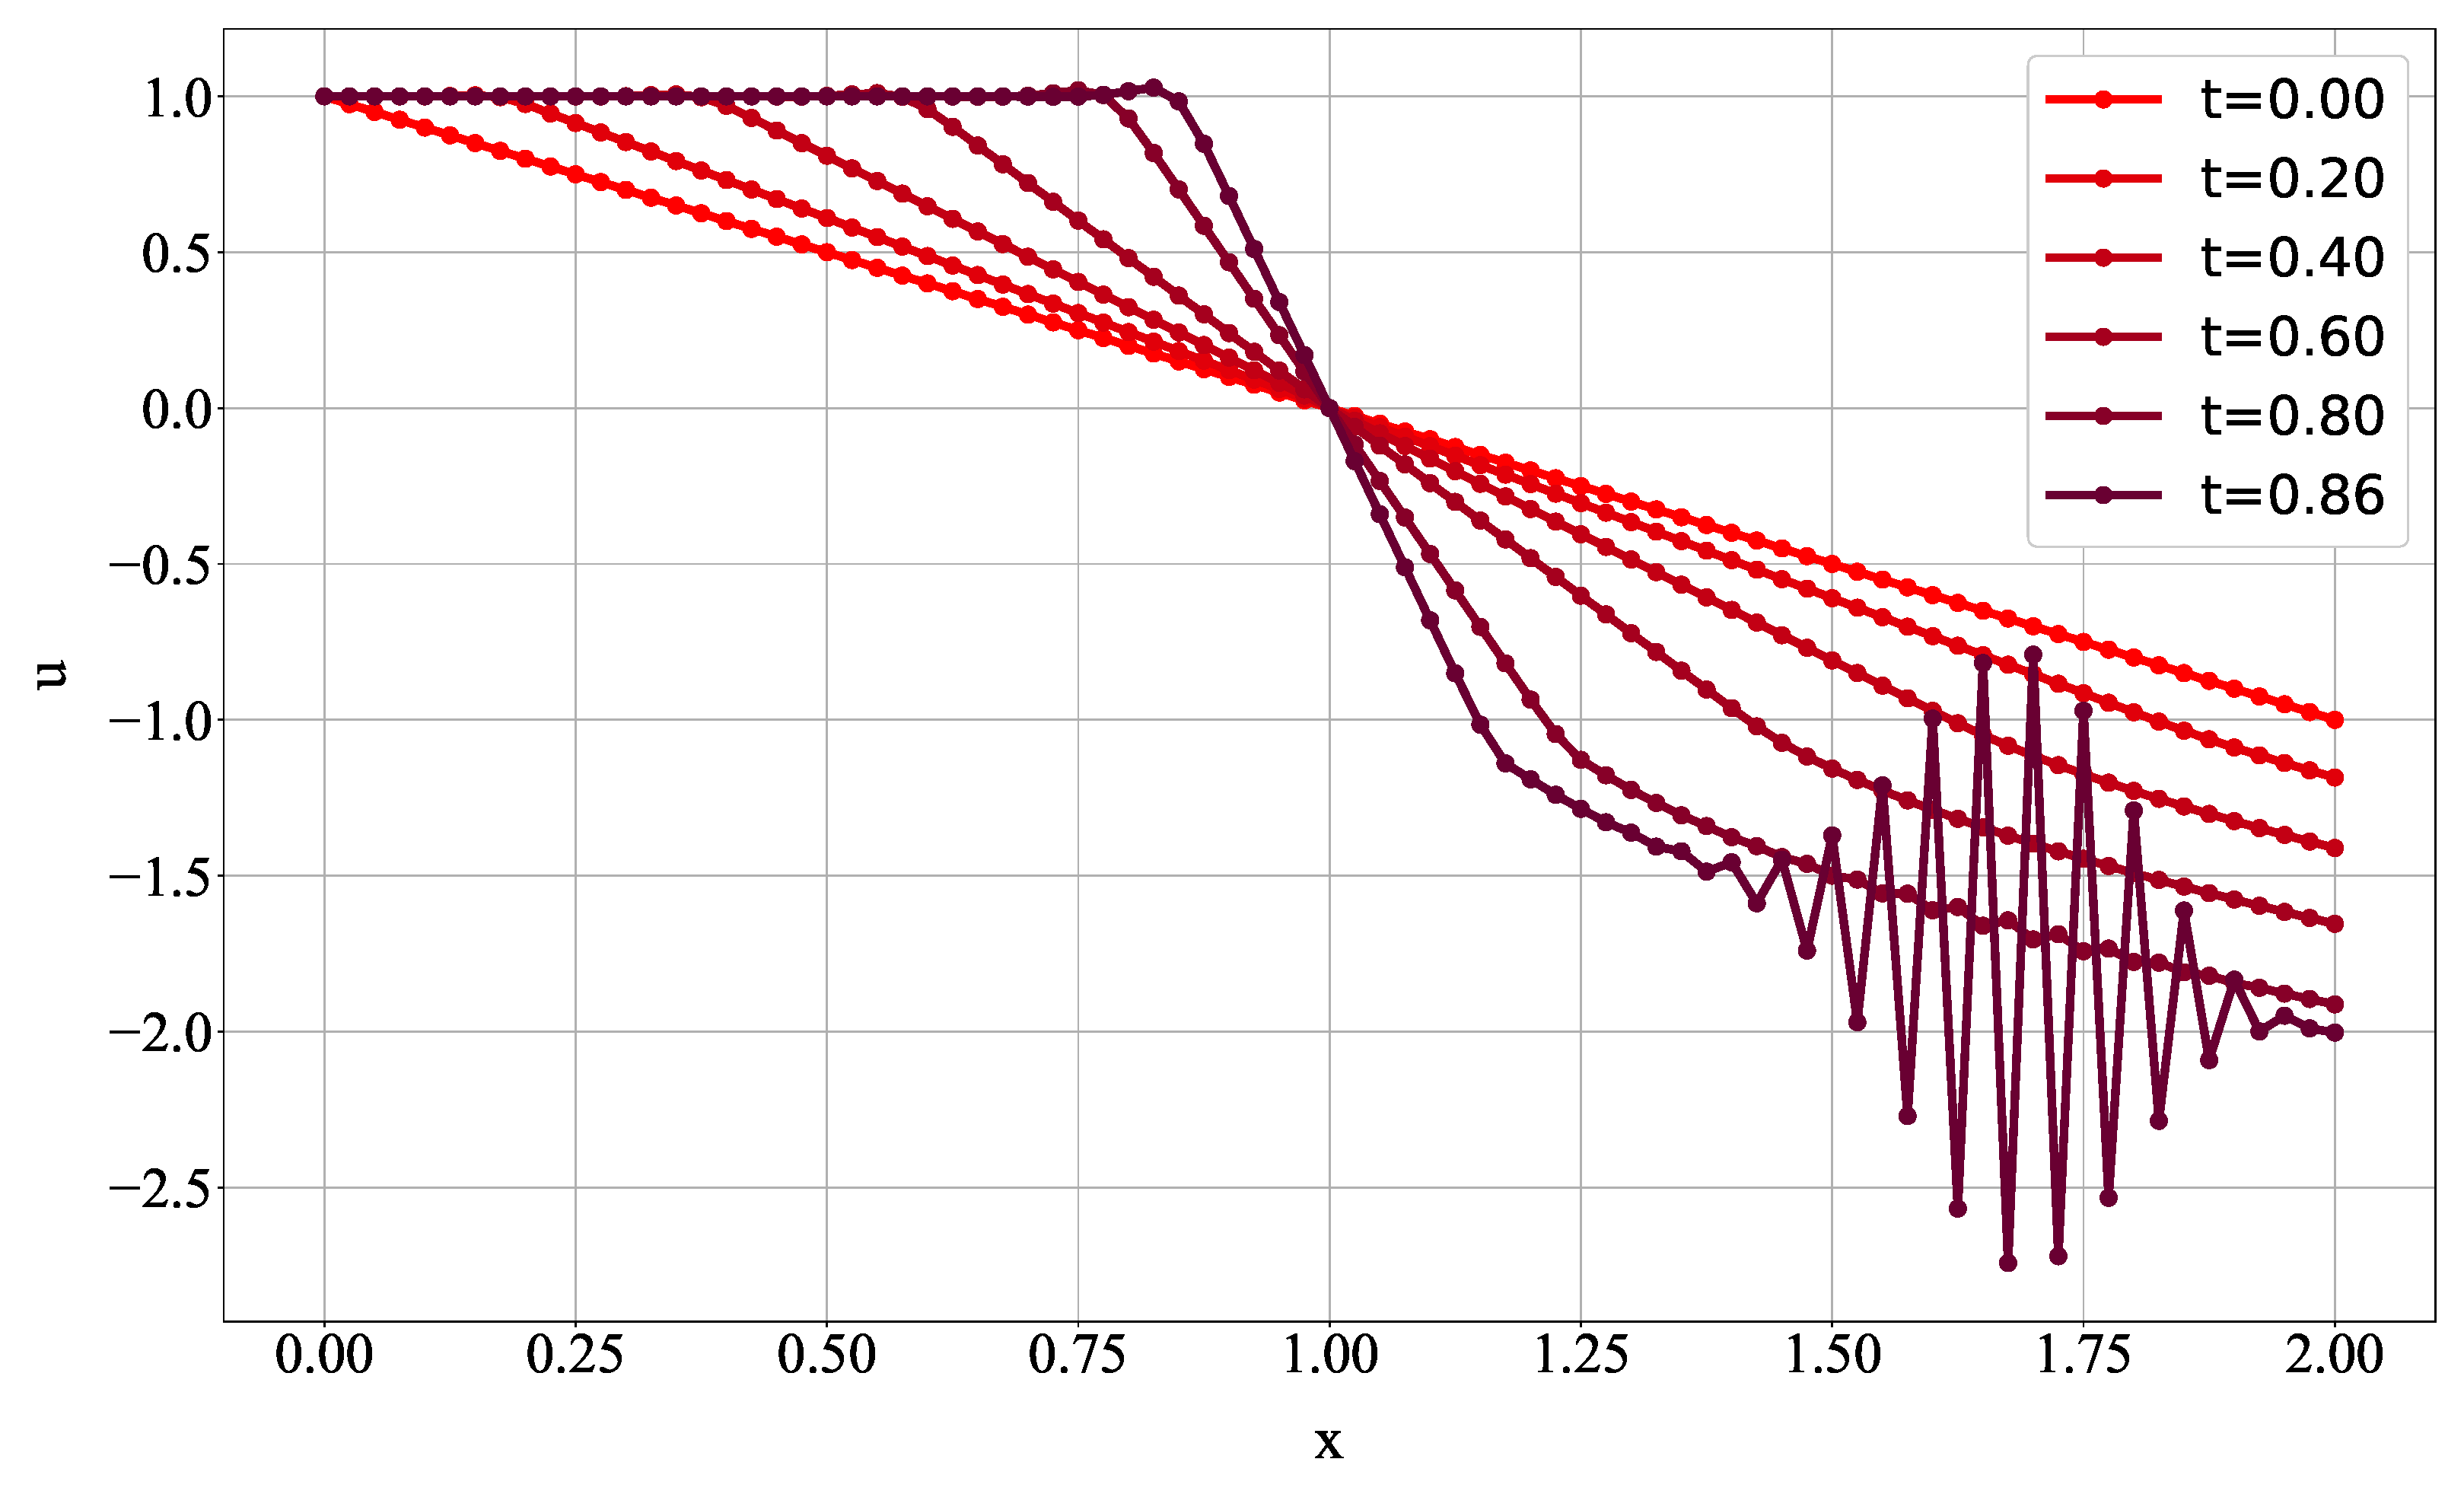
\includegraphics[width=0.425\linewidth]{4.lax-vendroff.cour09.f1025}}\\
      \midrule
      \multirow{2}{*}{\vspace{\myvspaceOne}$f_2$} & $0.5$    &
        \raisebox{-0.5\totalheight}{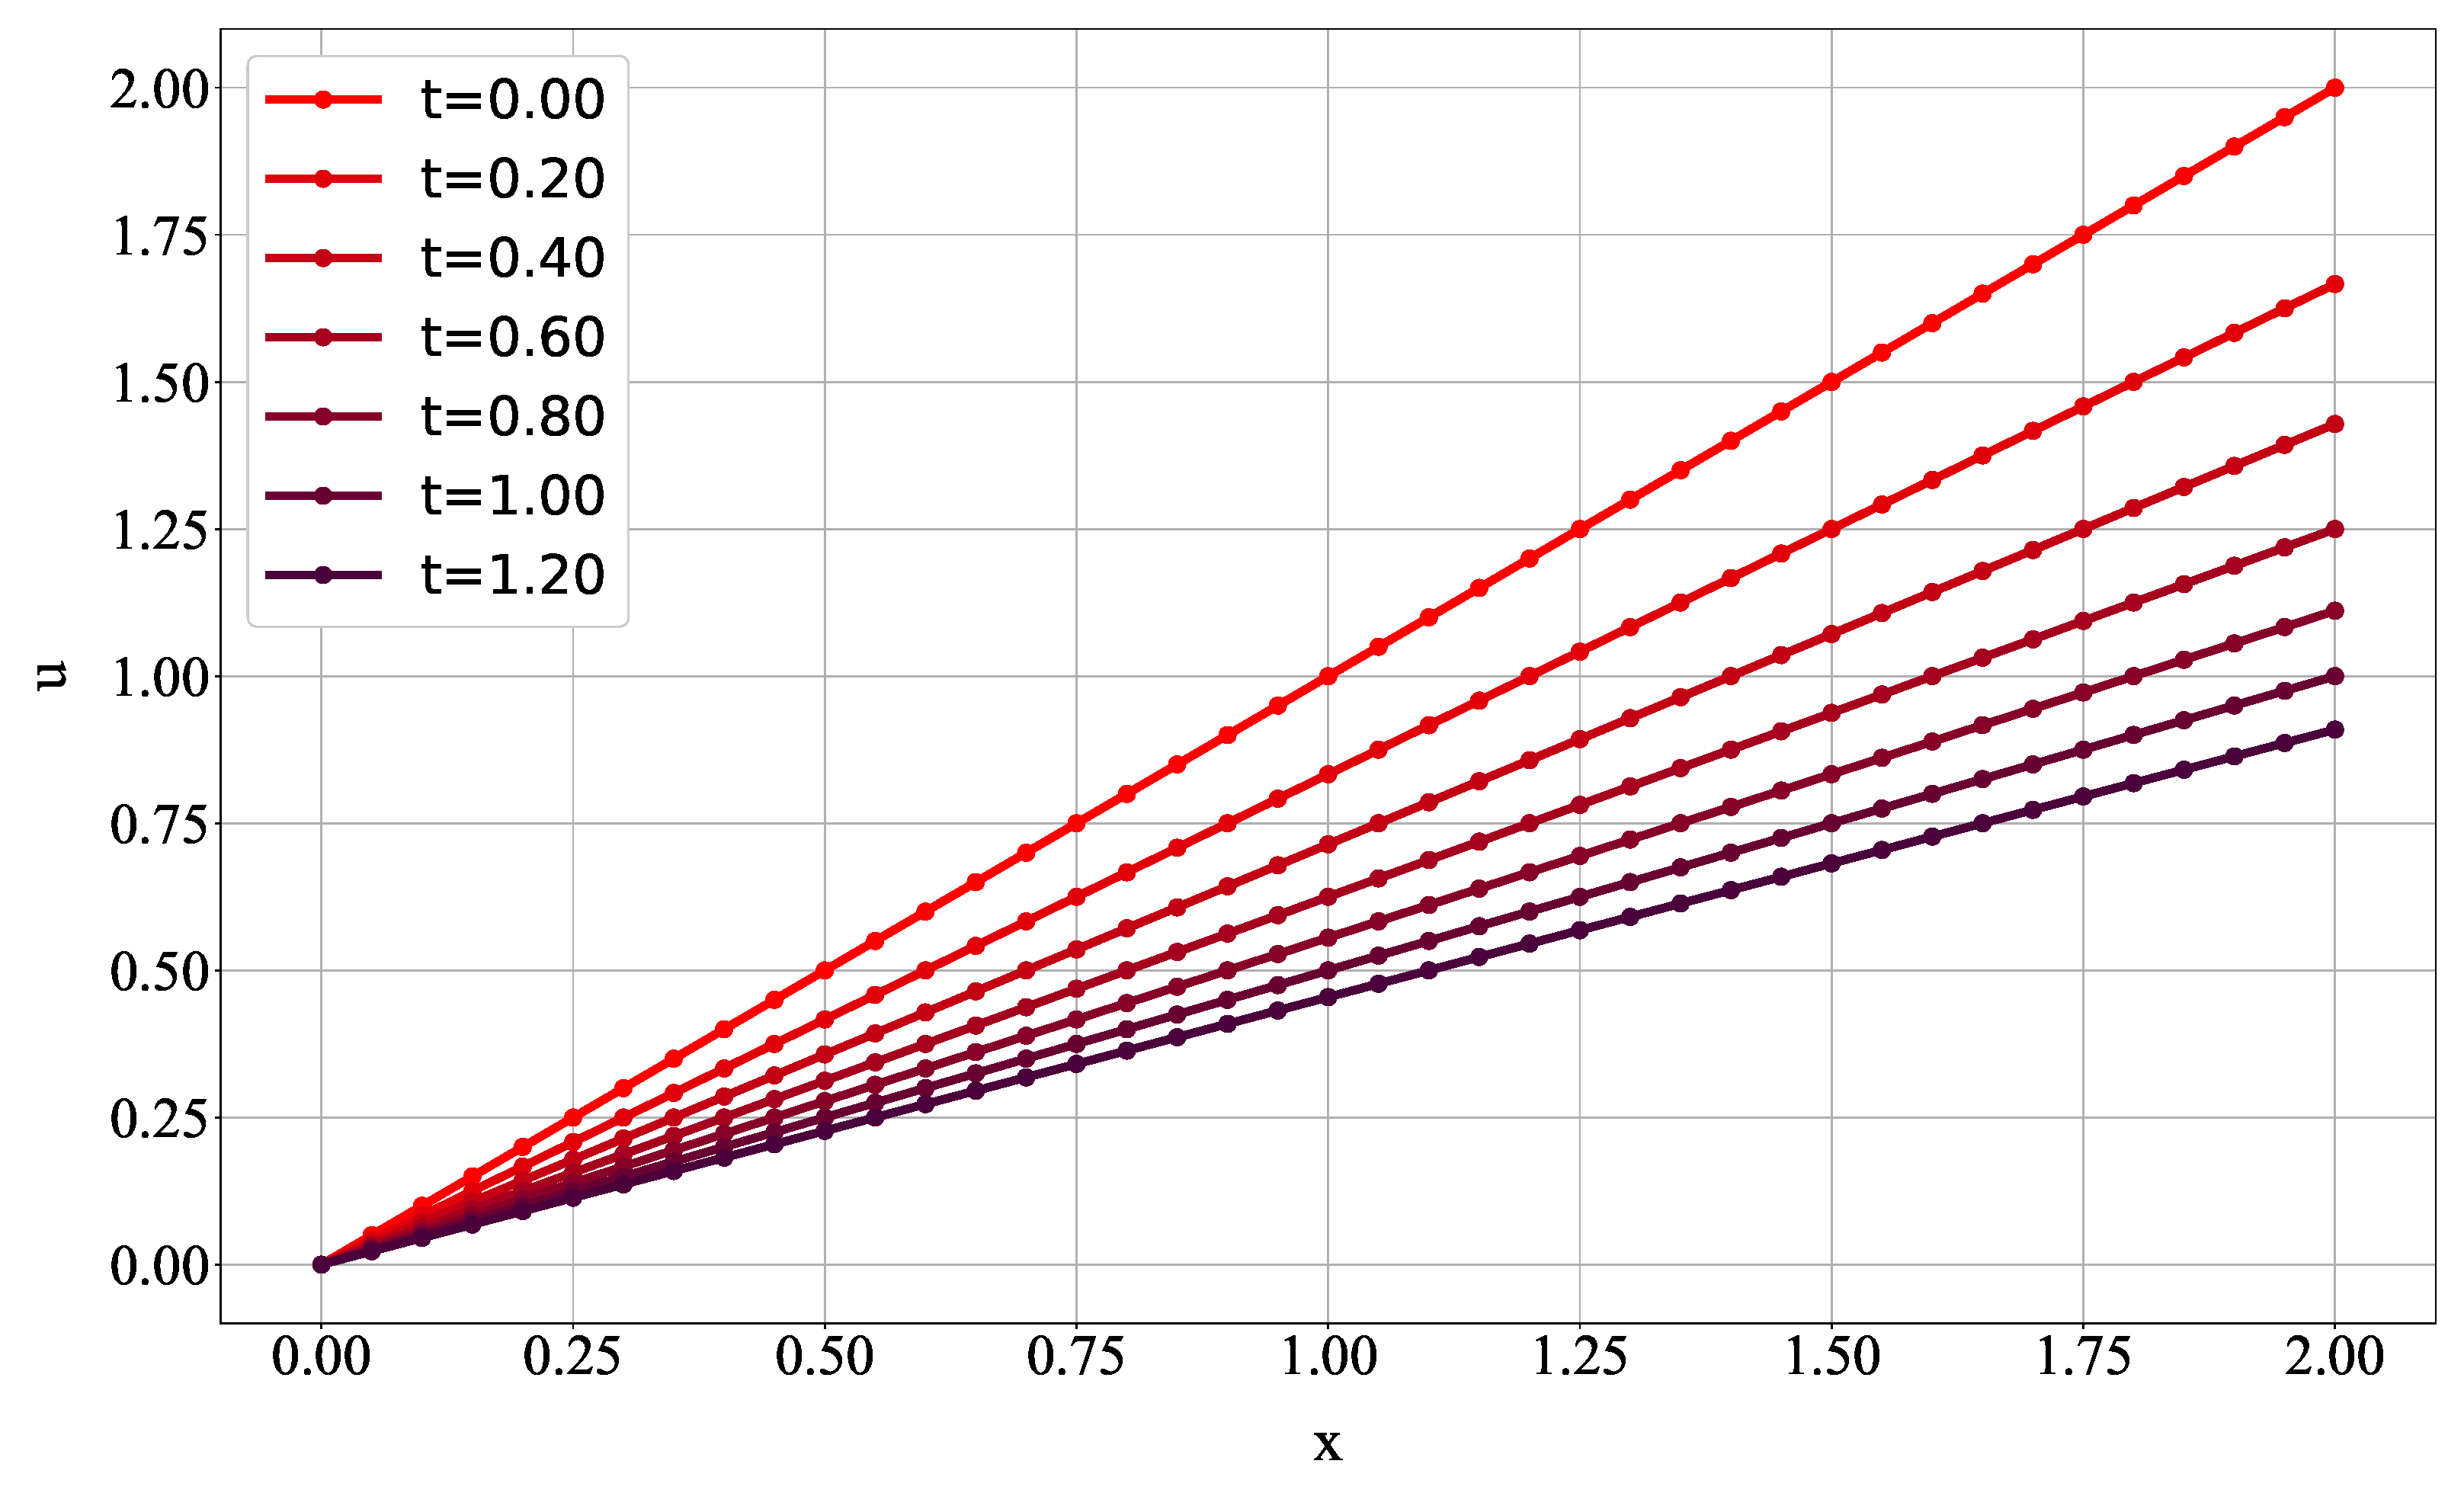
\includegraphics[width=0.425\linewidth]{4.lax-vendroff.cour05.f2050}} &
        \raisebox{-0.5\totalheight}{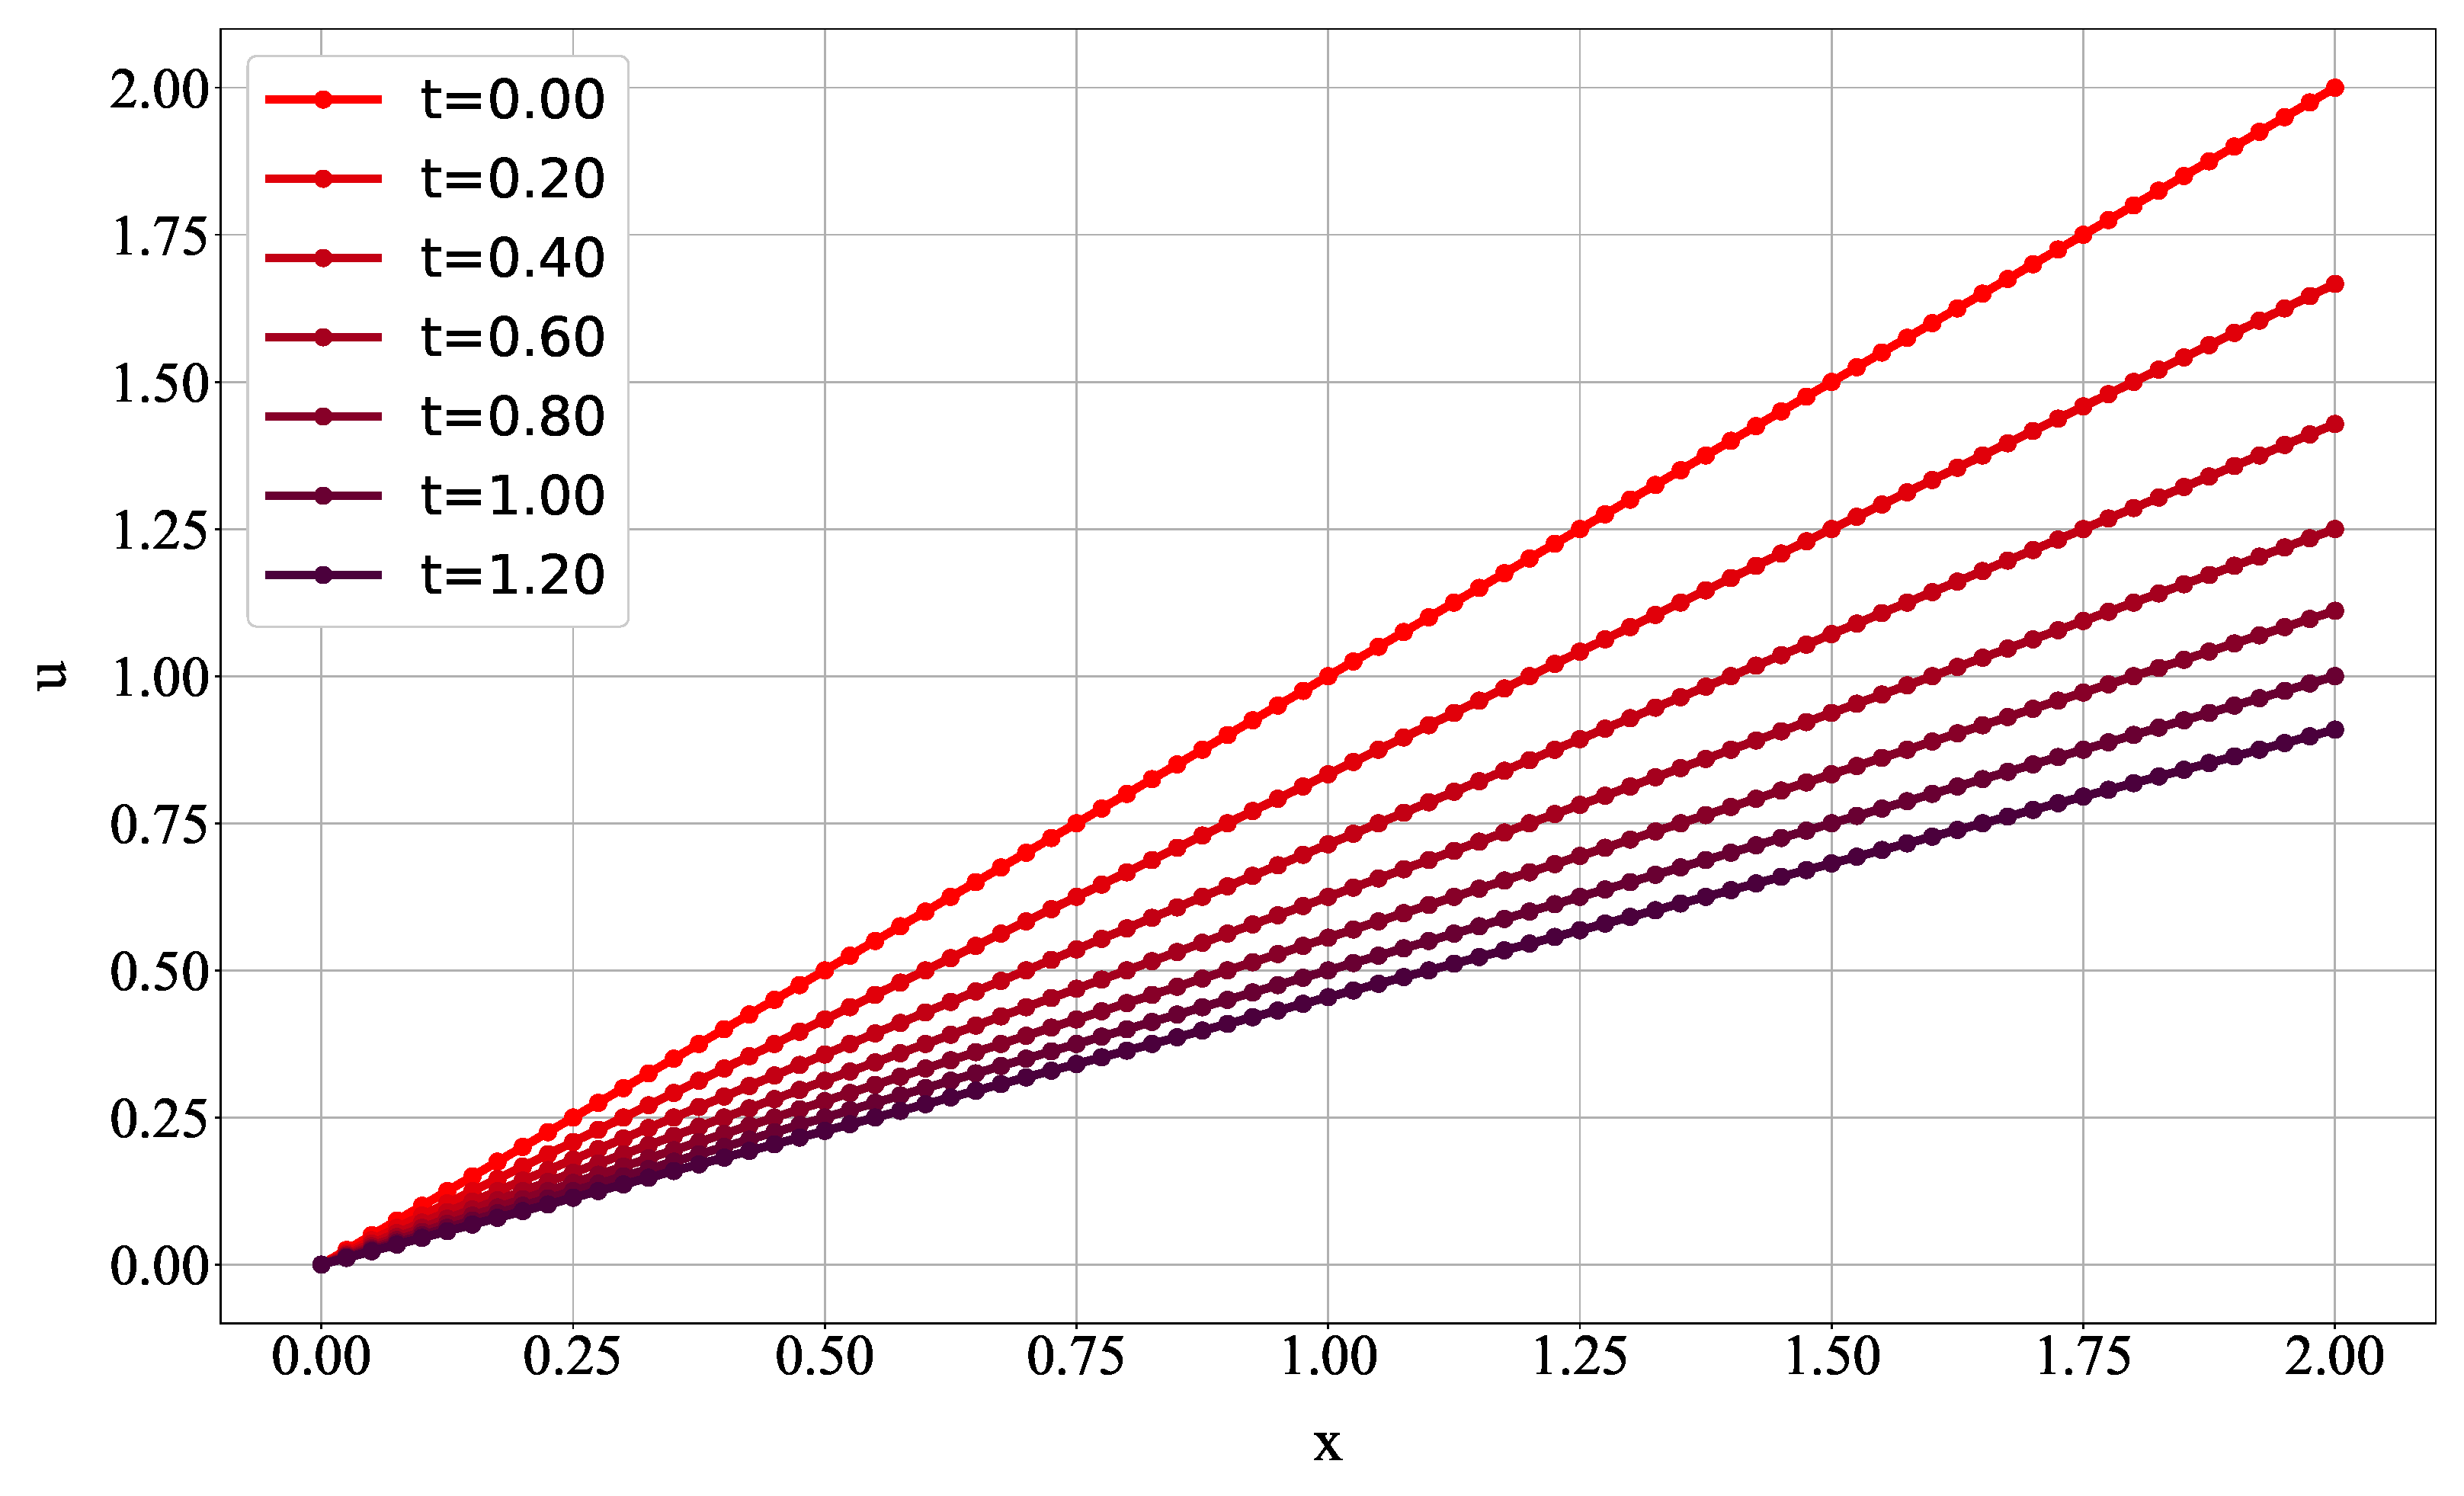
\includegraphics[width=0.425\linewidth]{4.lax-vendroff.cour05.f2025}}\\
      %\cmidrule{3-4}
      {}                                          & $0.9$    &
        \raisebox{-0.5\totalheight}{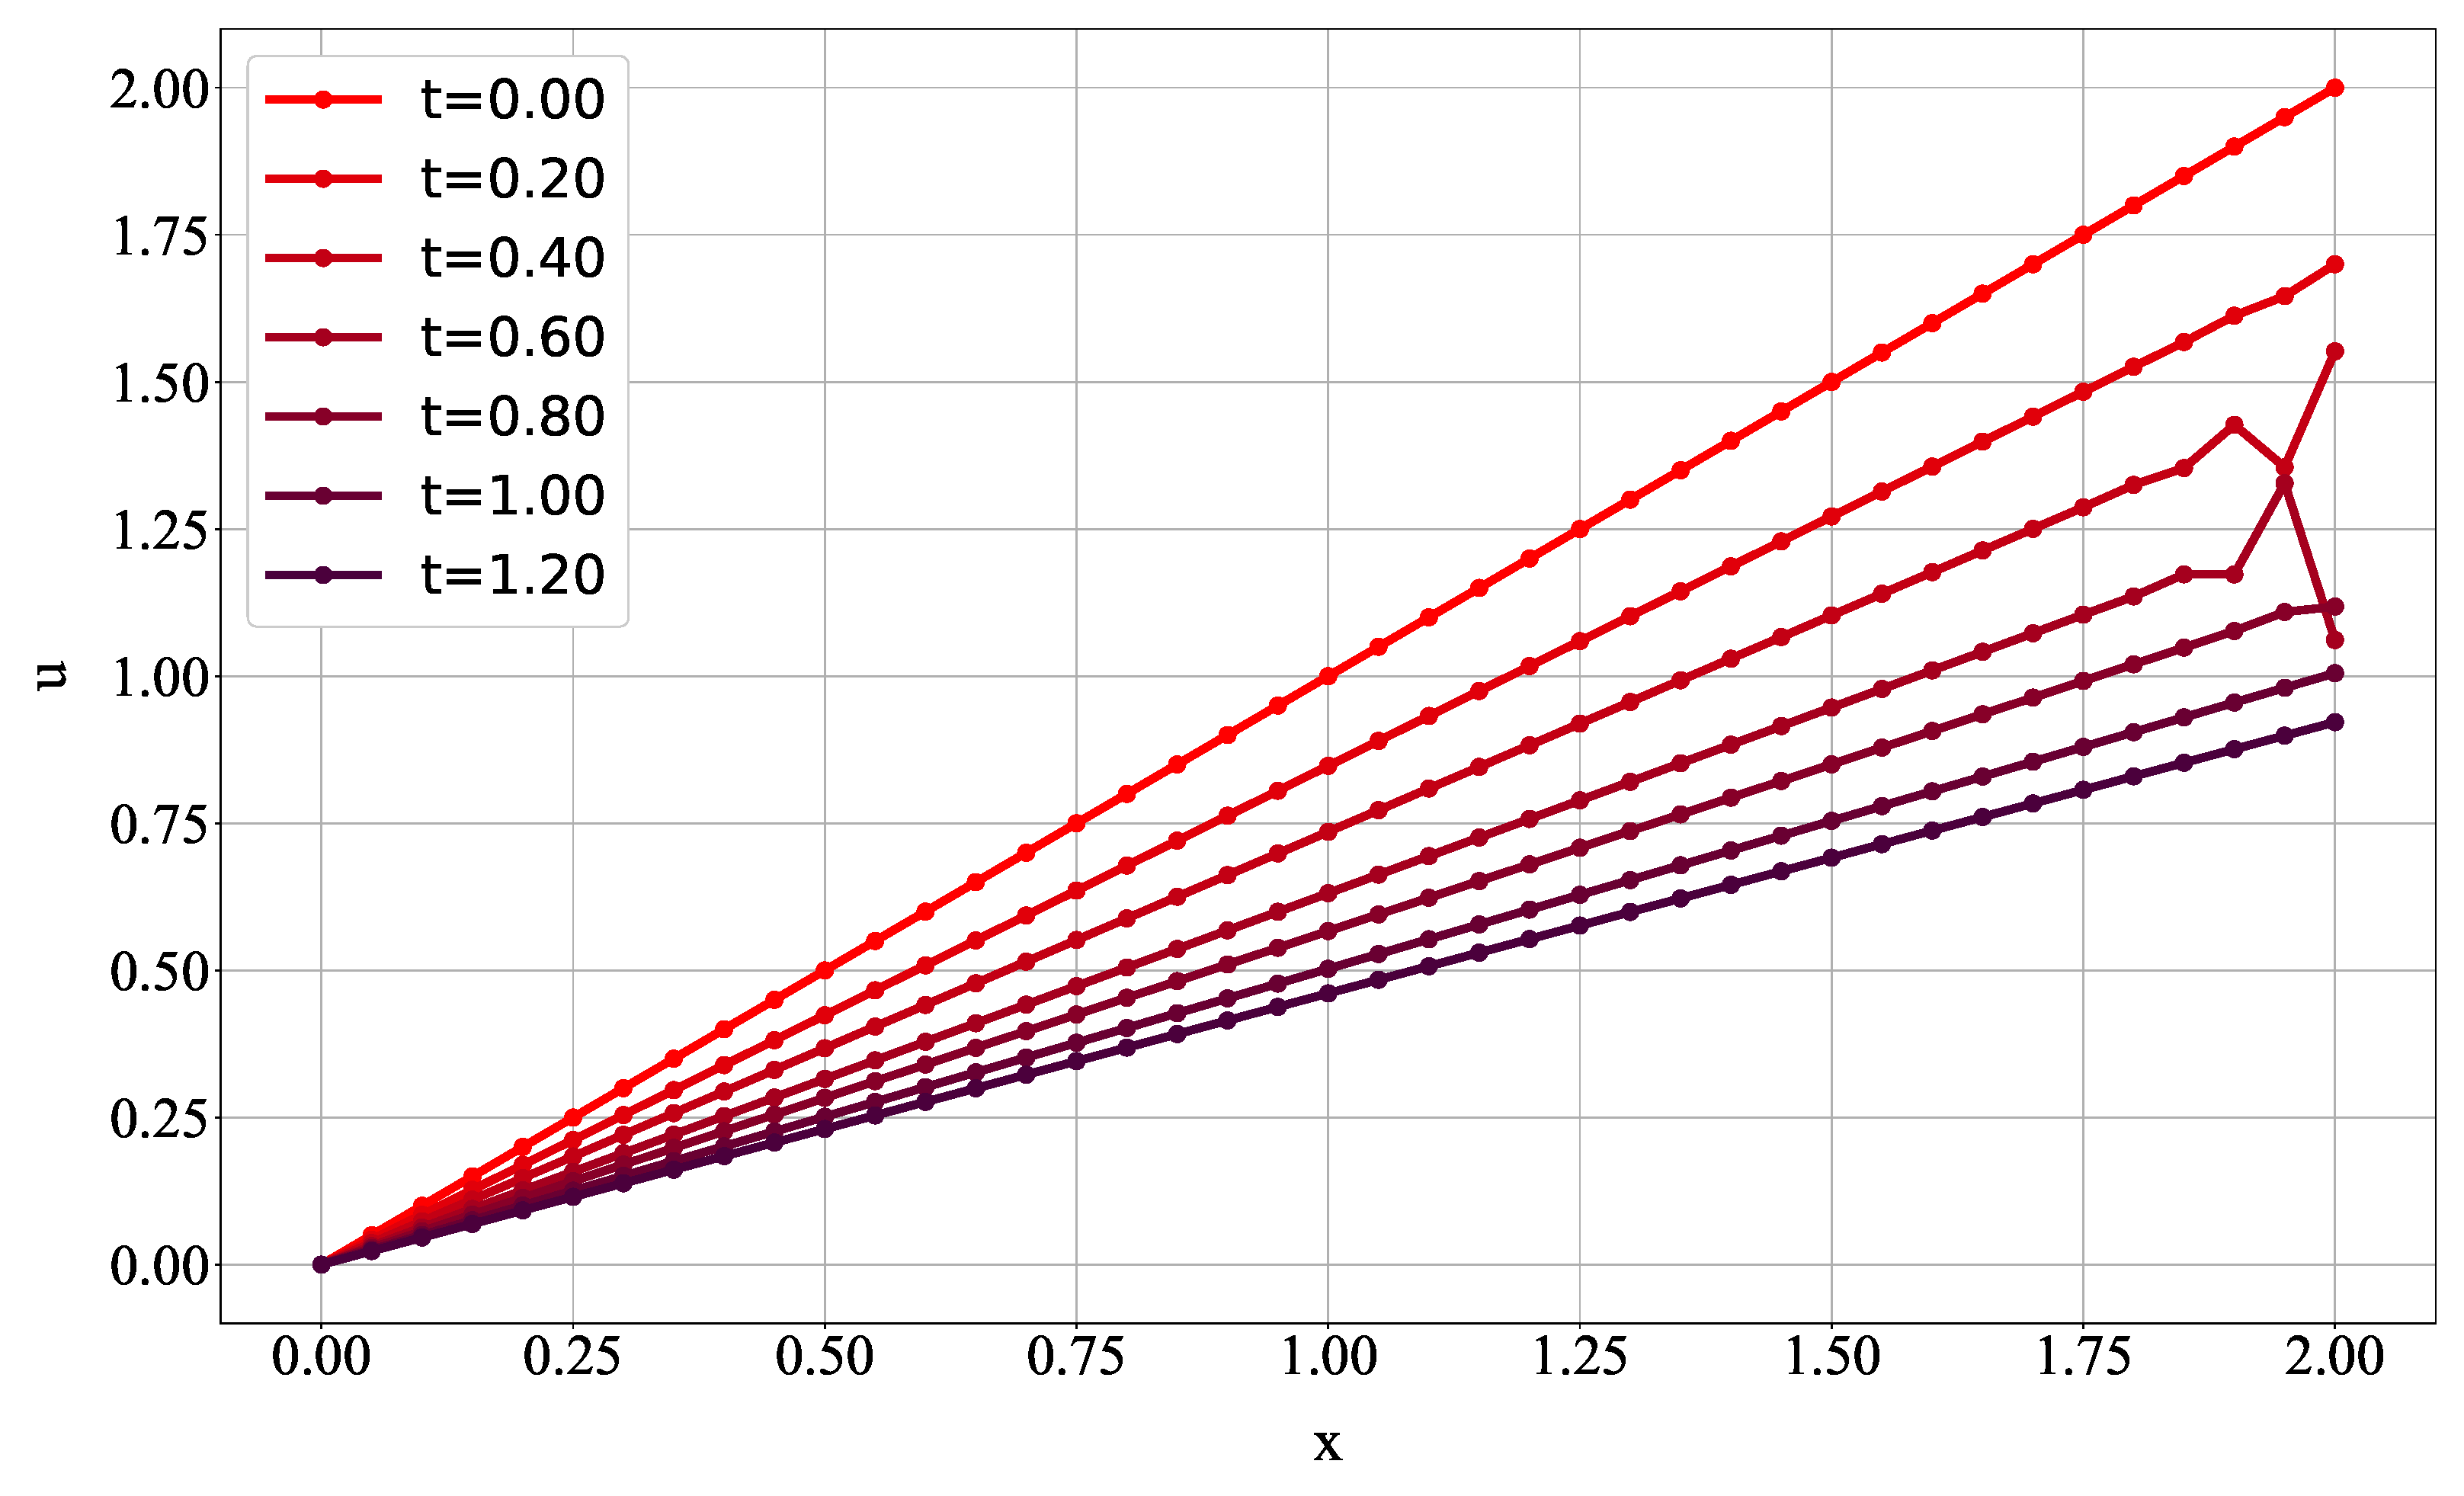
\includegraphics[width=0.425\linewidth]{4.lax-vendroff.cour09.f2050}} &
        \raisebox{-0.5\totalheight}{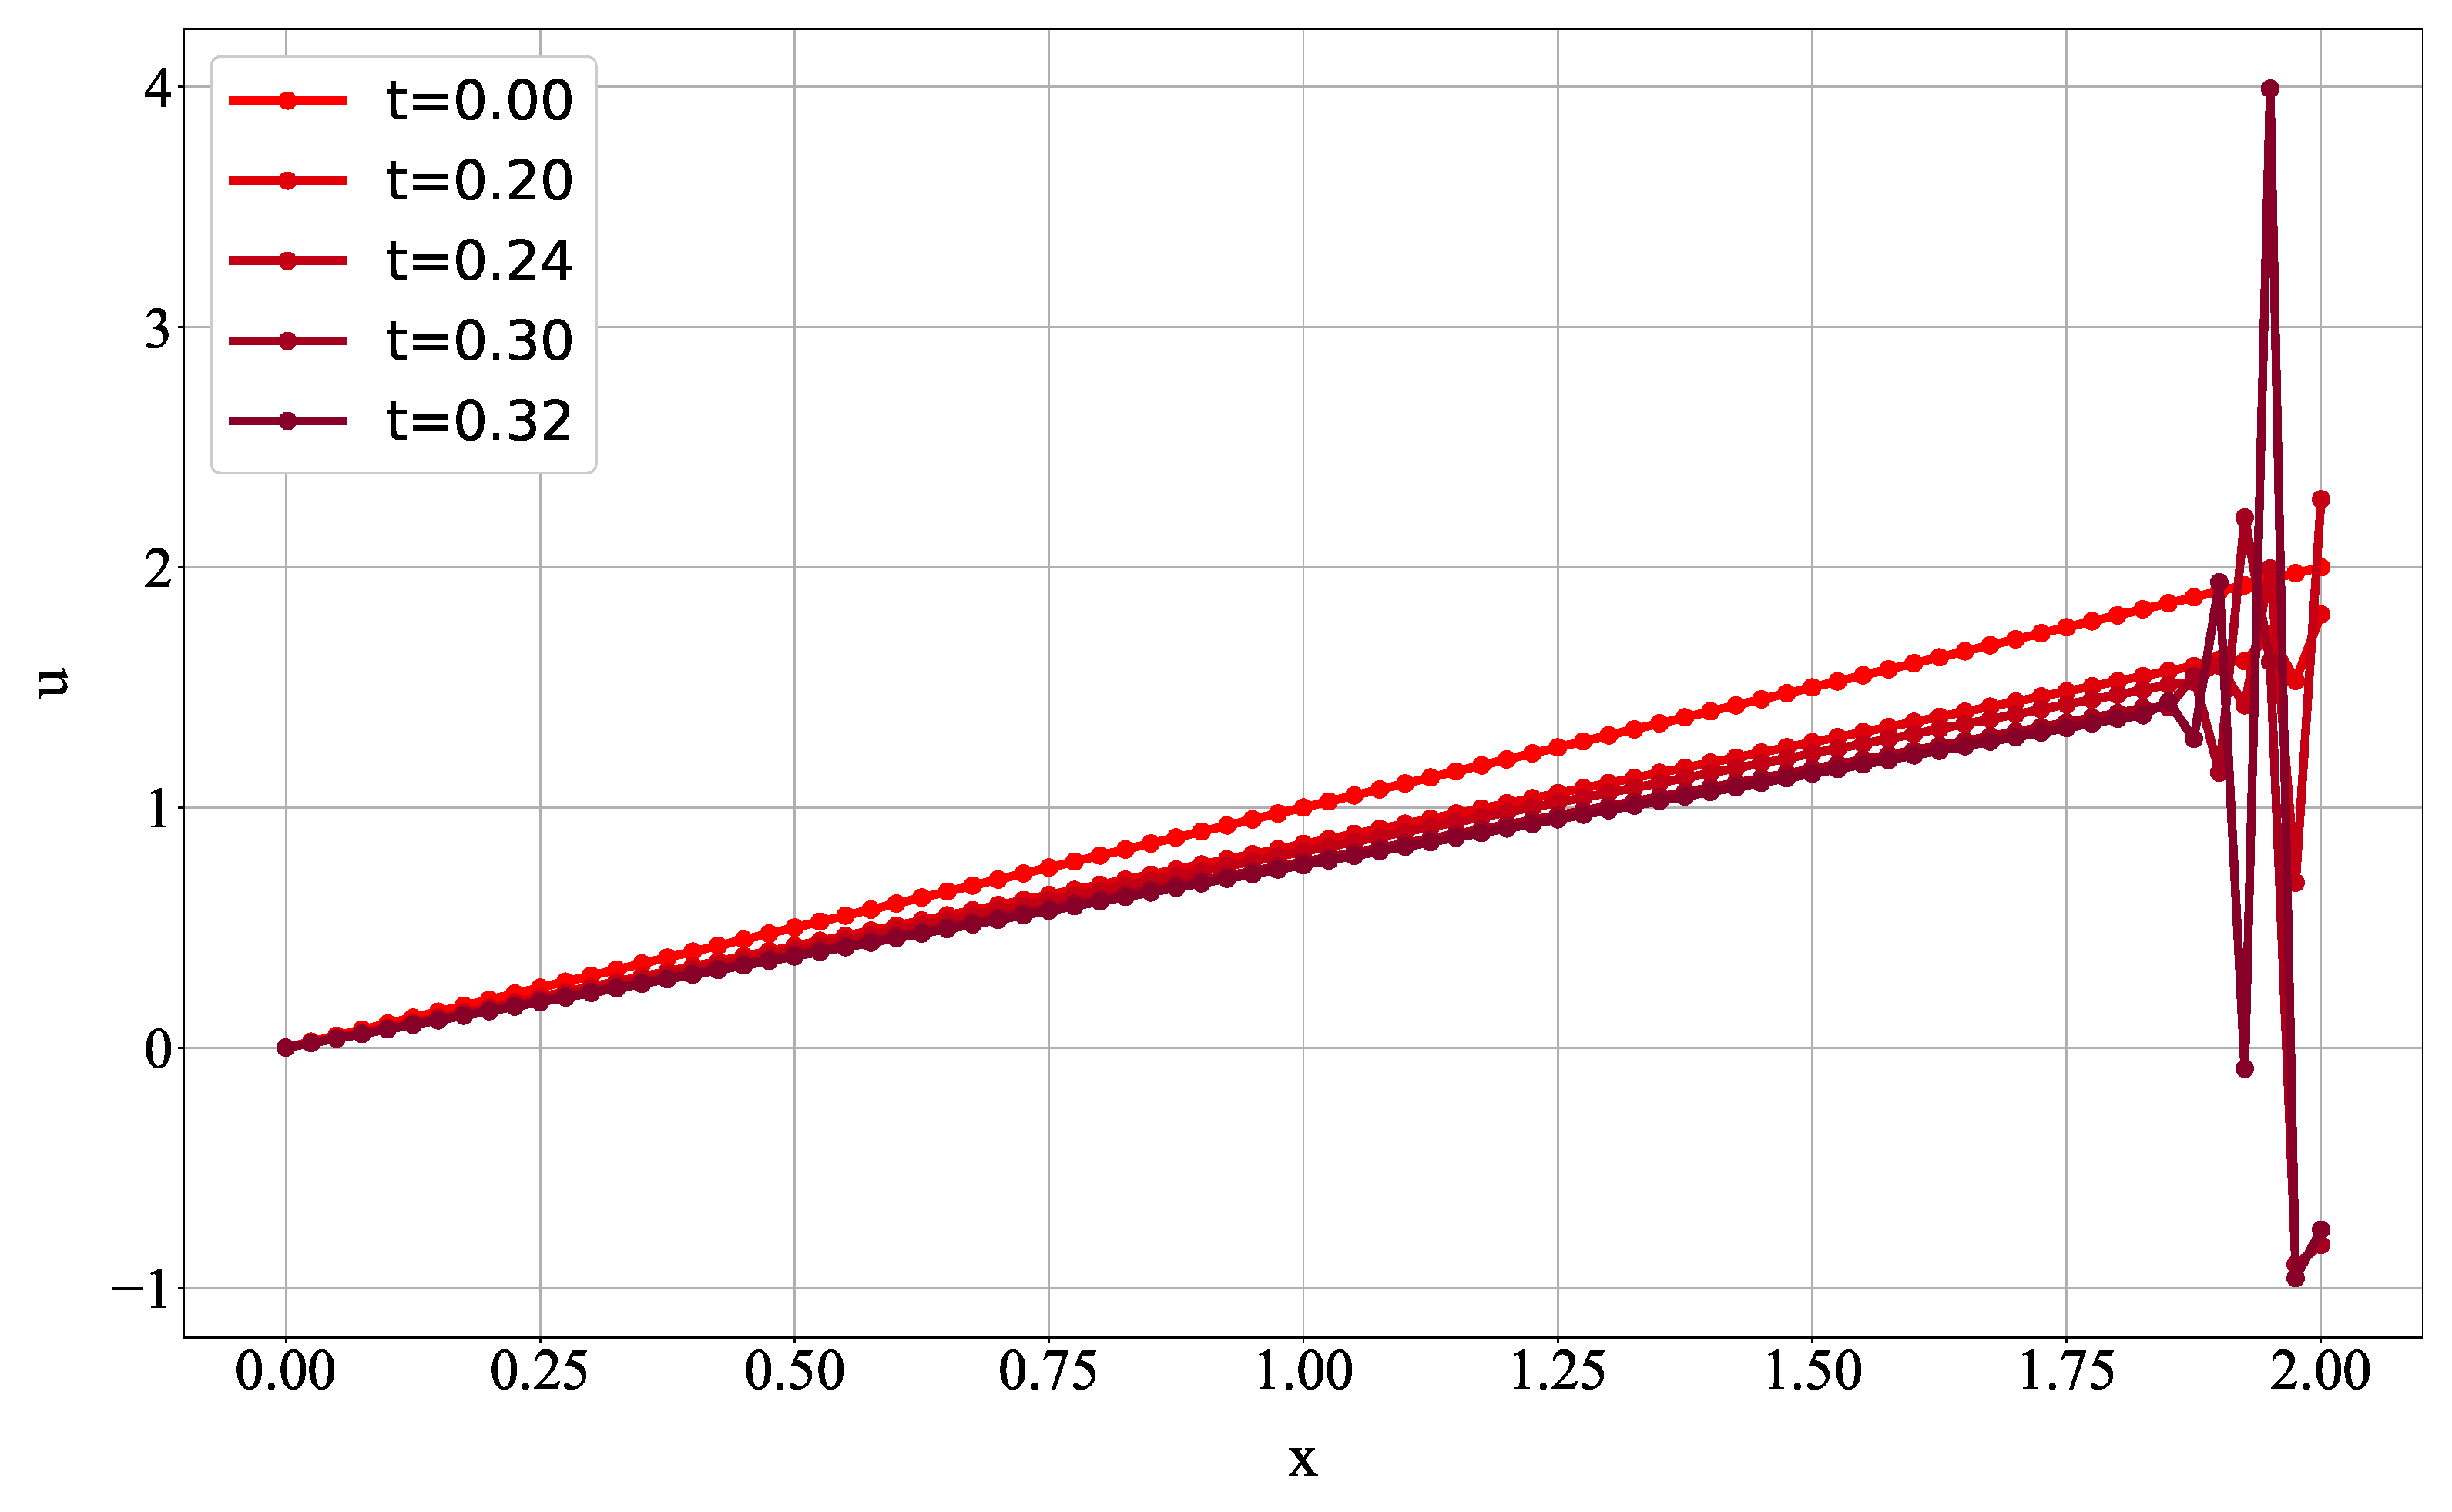
\includegraphics[width=0.425\linewidth]{4.lax-vendroff.cour09.f2025}}\\
      \bottomrule
    \end{tabular}
  \end{center}
  \end{table}
  
  \begin{table}[p]
  \caption{"`МакКормак"' (\ref{sec:maccormack})}
  \label{plot:maccormack}
  \begin{center}
    \begin{tabular}{c c c c}
      \toprule
      {$f$}                                       & $\sigma$ & $h_1$ & $h_2$\\
      \midrule
      \multirow{2}{*}{\vspace{\myvspaceOne}$f_1$} & $0.5$    & 
        \raisebox{-0.5\totalheight}{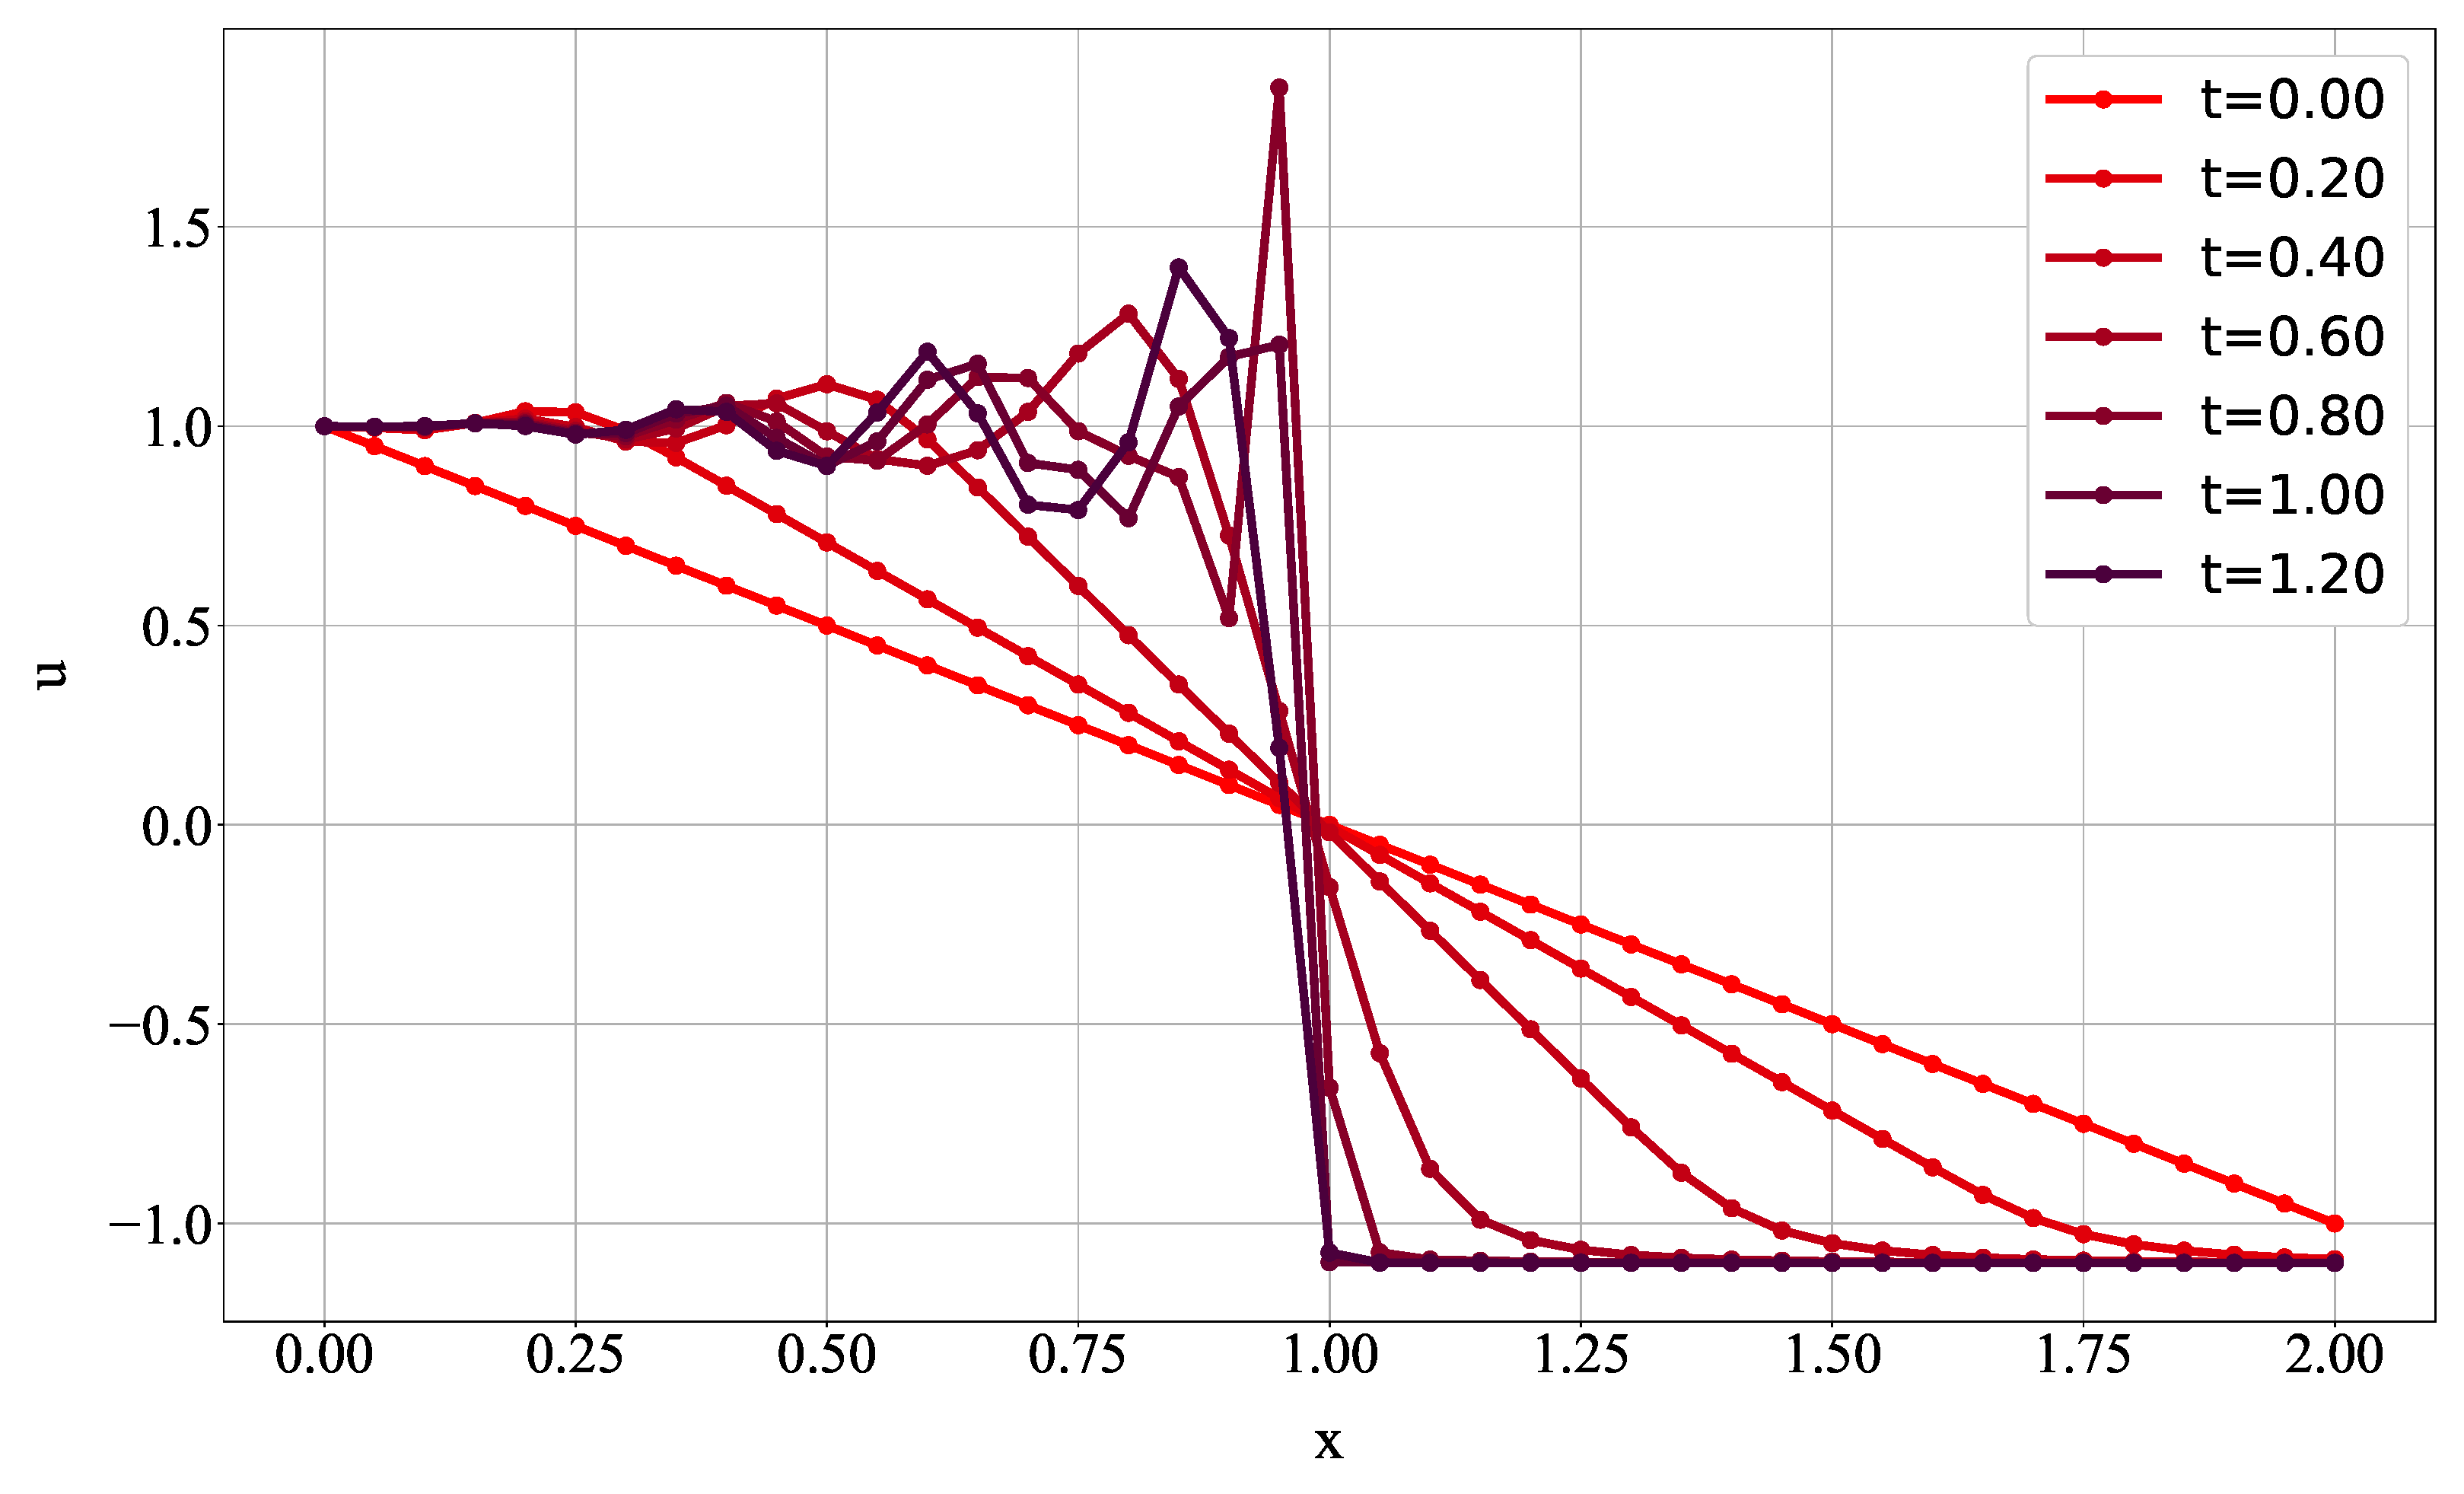
\includegraphics[width=0.425\linewidth]{5.maccormack.cour05.f1050}} &
        \raisebox{-0.5\totalheight}{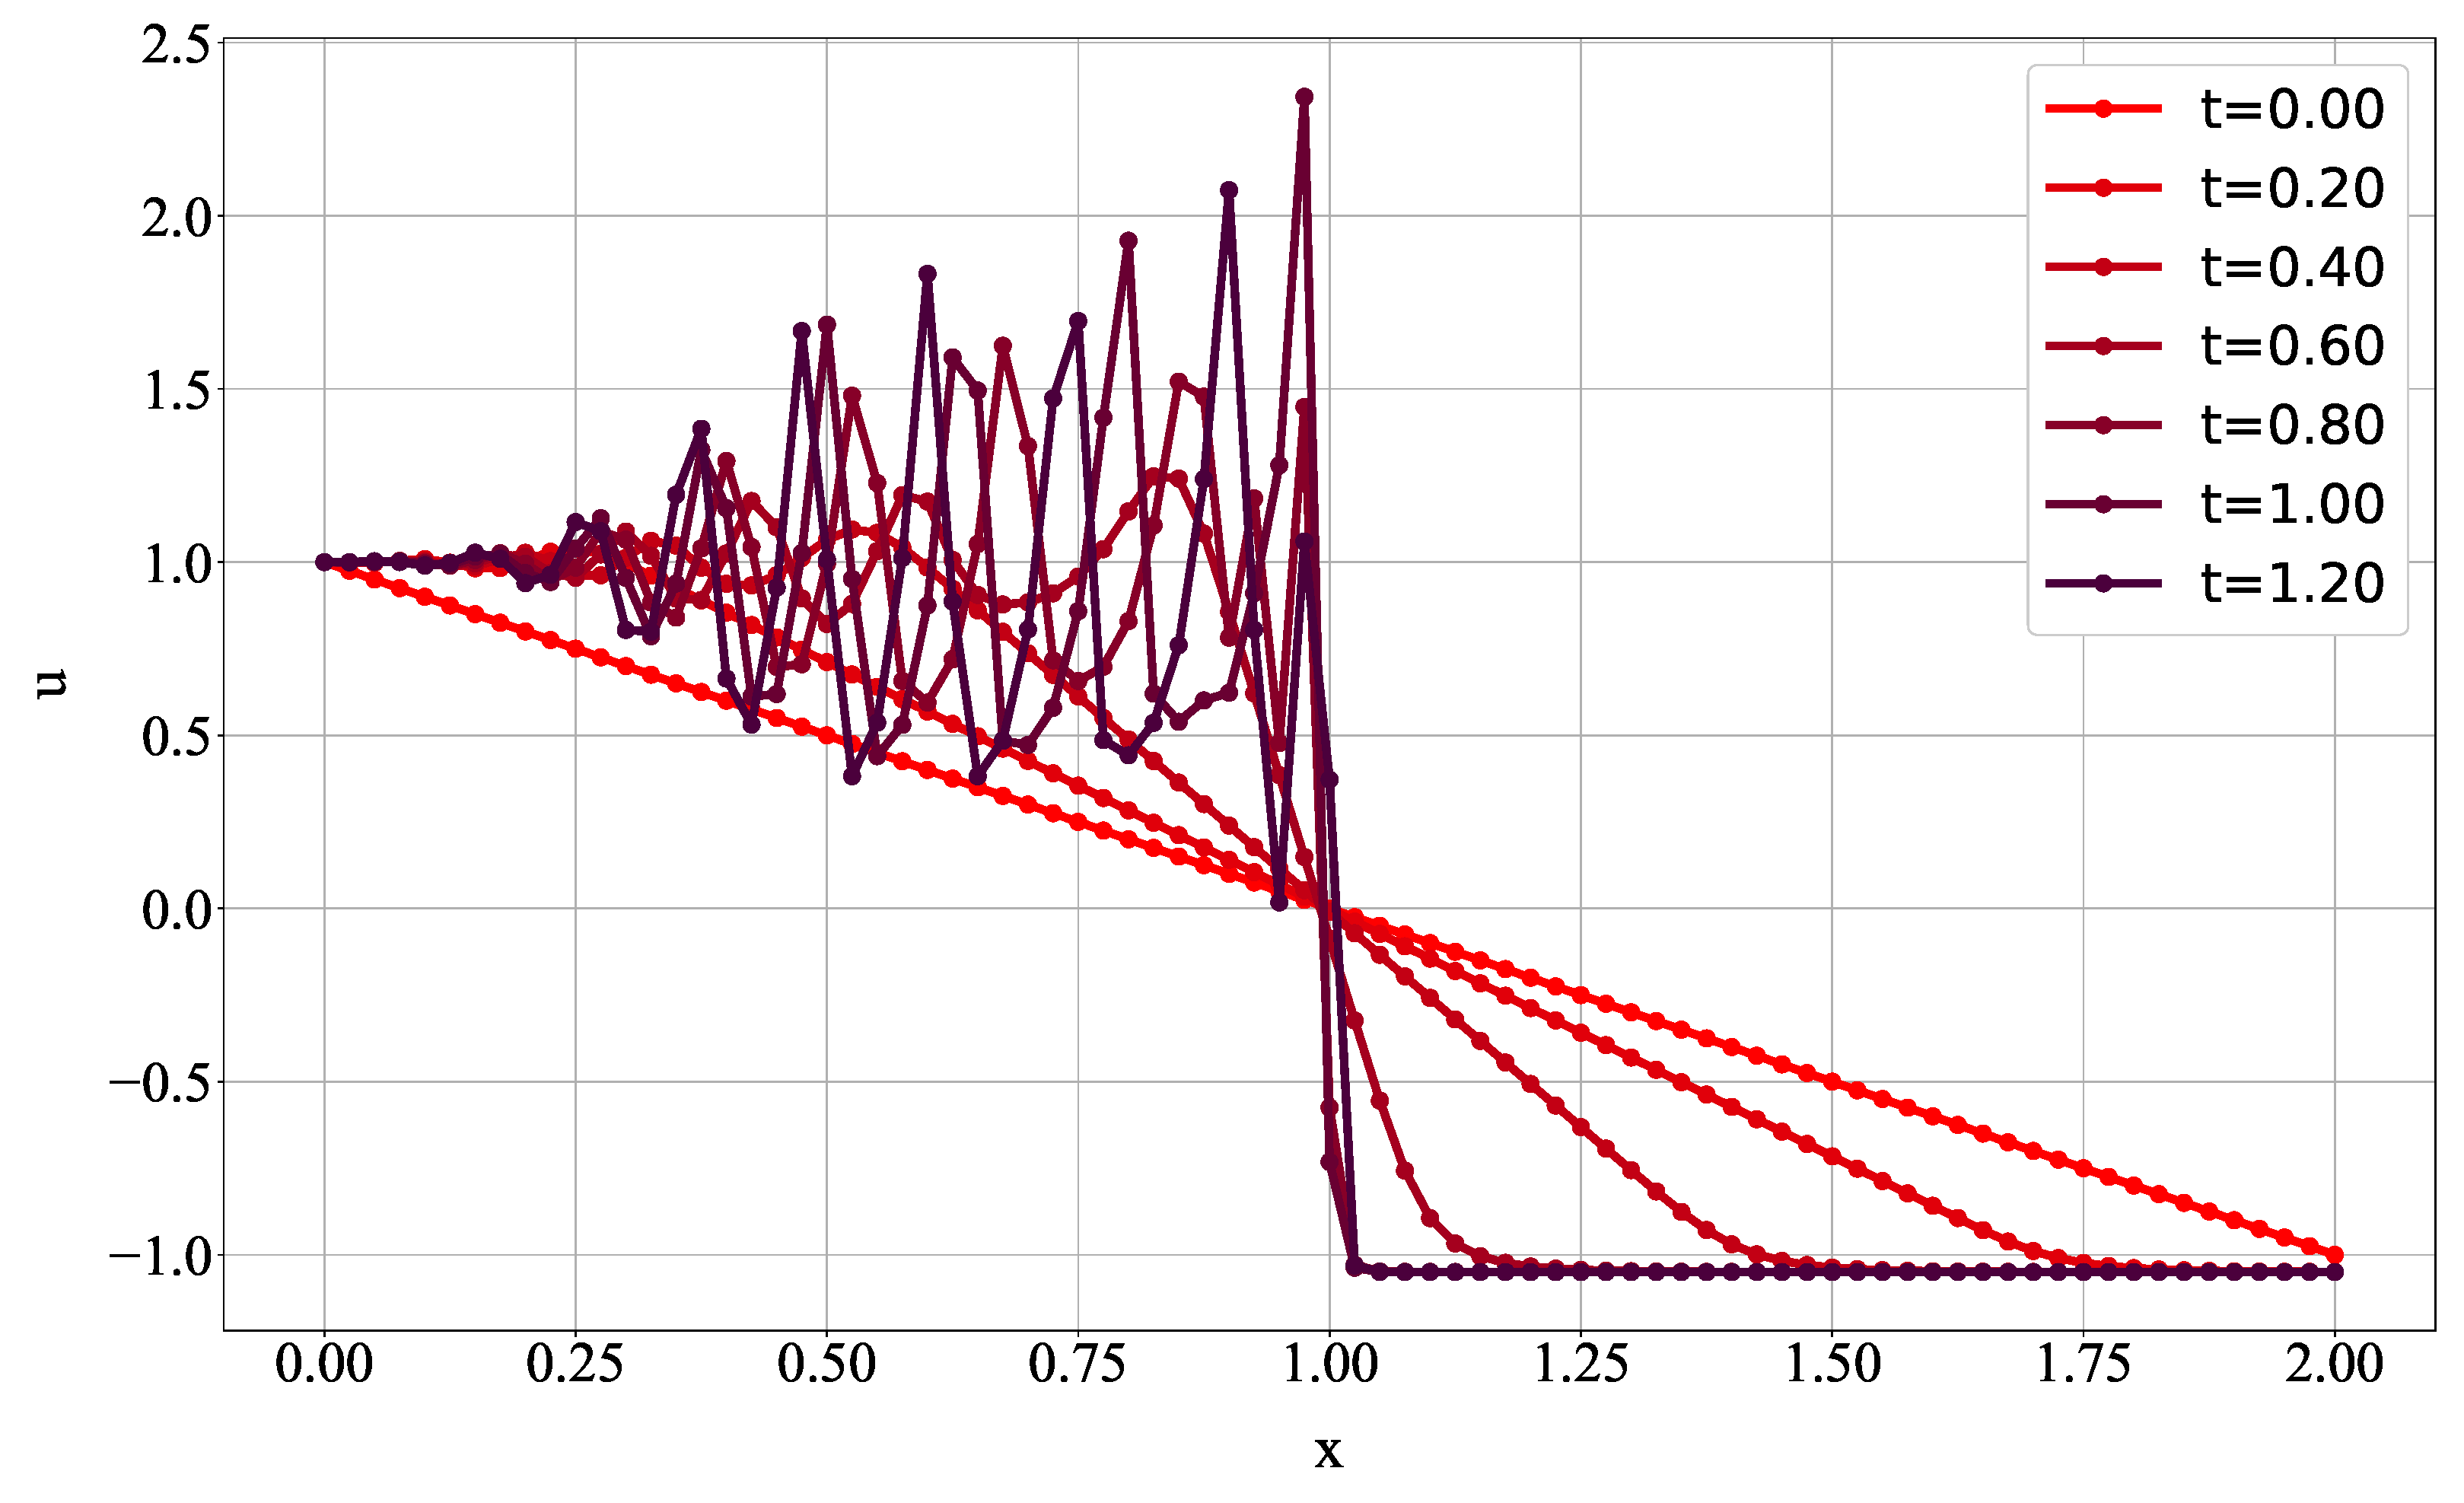
\includegraphics[width=0.425\linewidth]{5.maccormack.cour05.f1025}}\\
      %\cmidrule{3-4}
      {}                                          & $0.9$    &
        \raisebox{-0.5\totalheight}{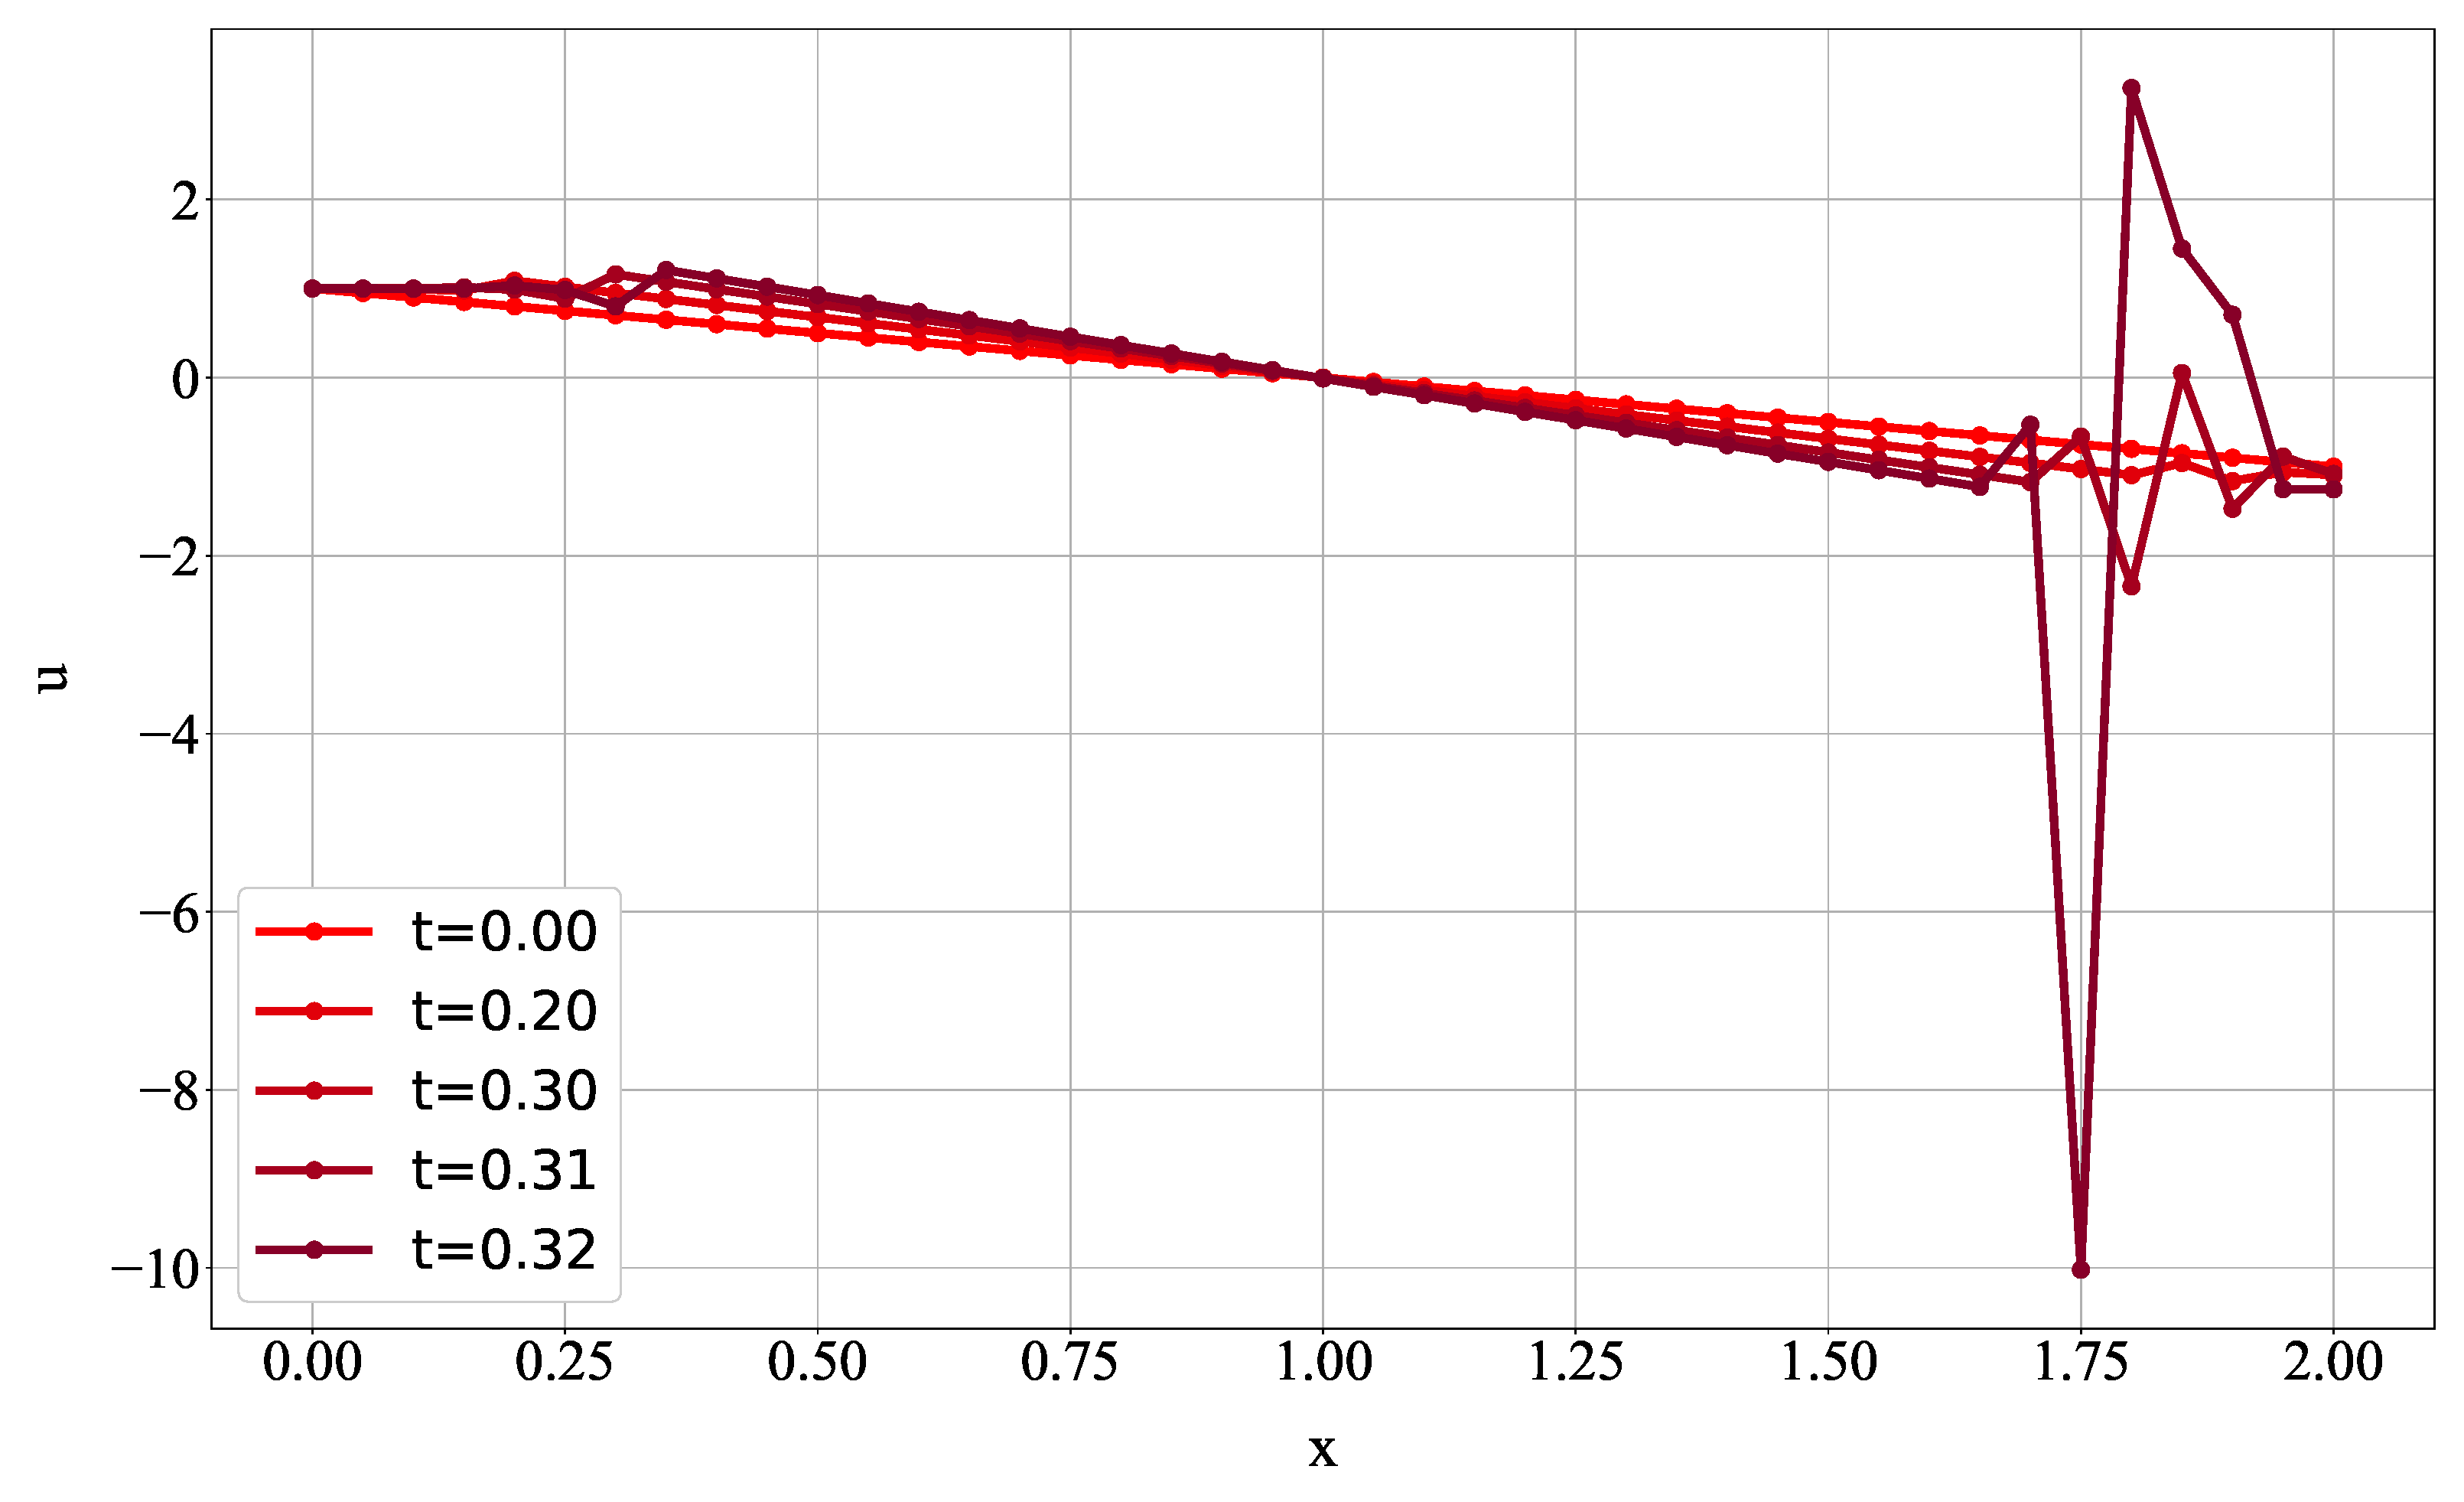
\includegraphics[width=0.425\linewidth]{5.maccormack.cour09.f1050}} & 
        \raisebox{-0.5\totalheight}{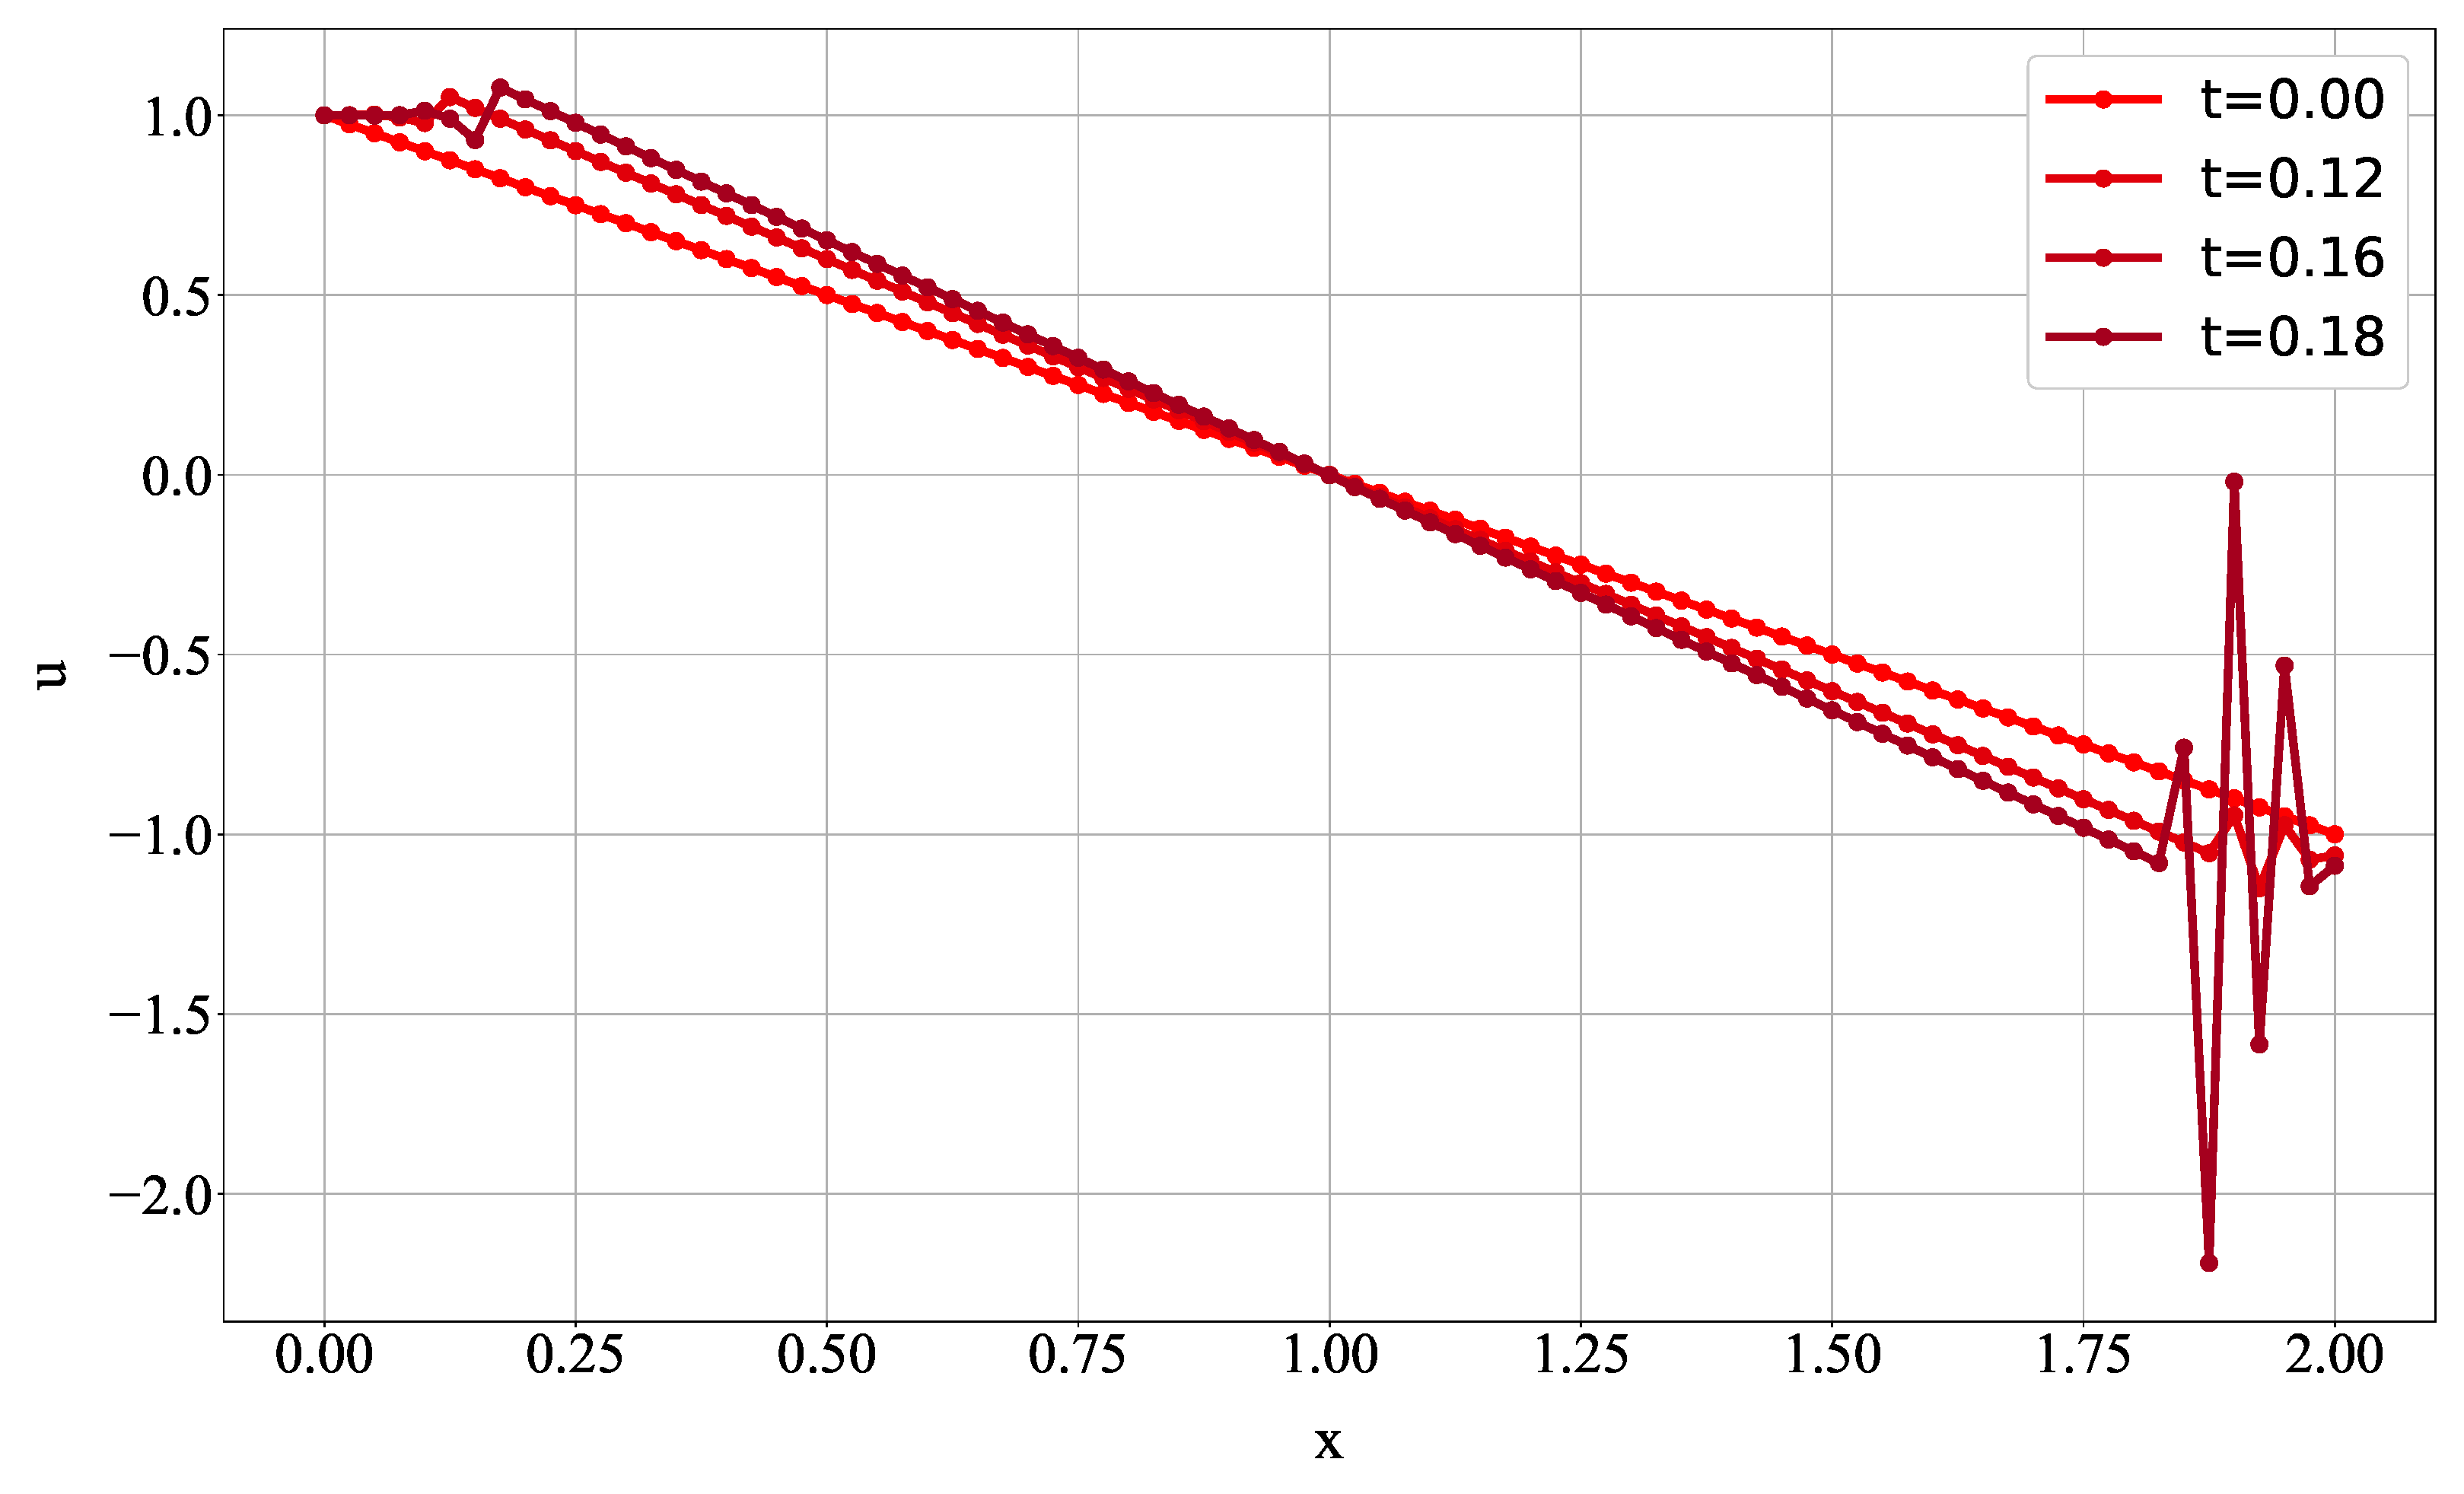
\includegraphics[width=0.425\linewidth]{5.maccormack.cour09.f1025}}\\
      \midrule
      \multirow{2}{*}{\vspace{\myvspaceOne}$f_2$} & $0.5$    &
        \raisebox{-0.5\totalheight}{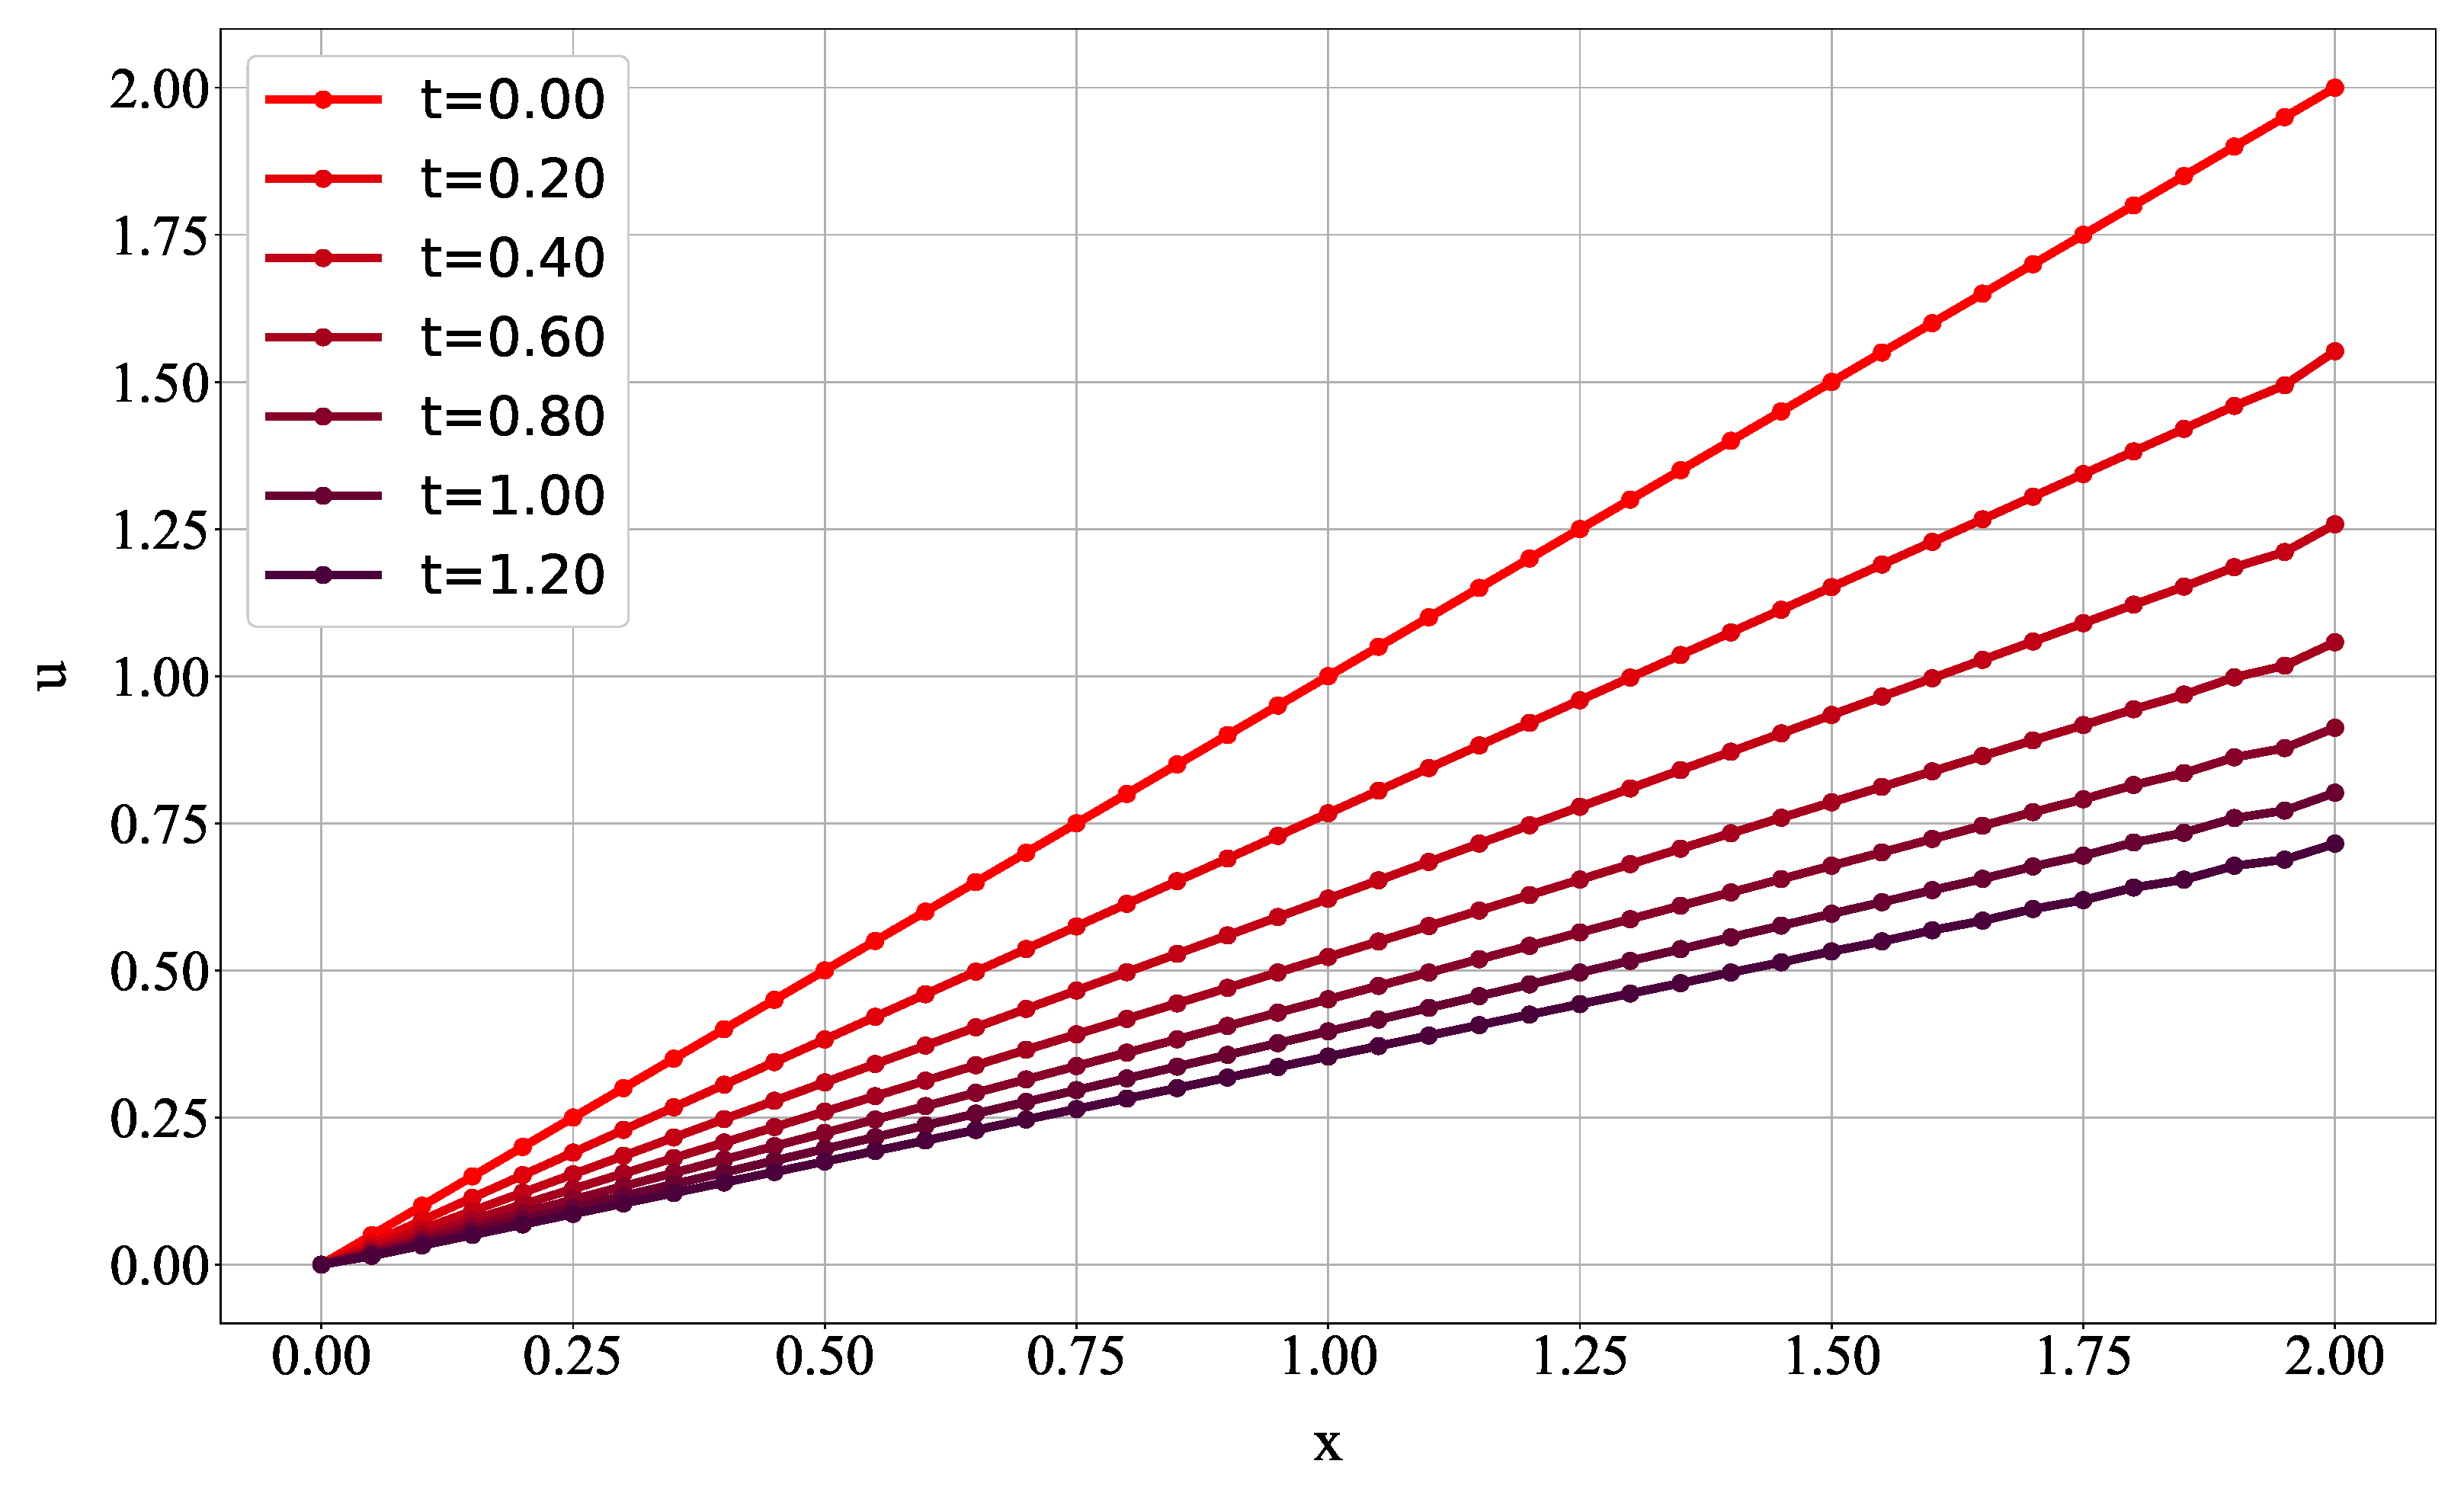
\includegraphics[width=0.425\linewidth]{5.maccormack.cour05.f2050}} &
        \raisebox{-0.5\totalheight}{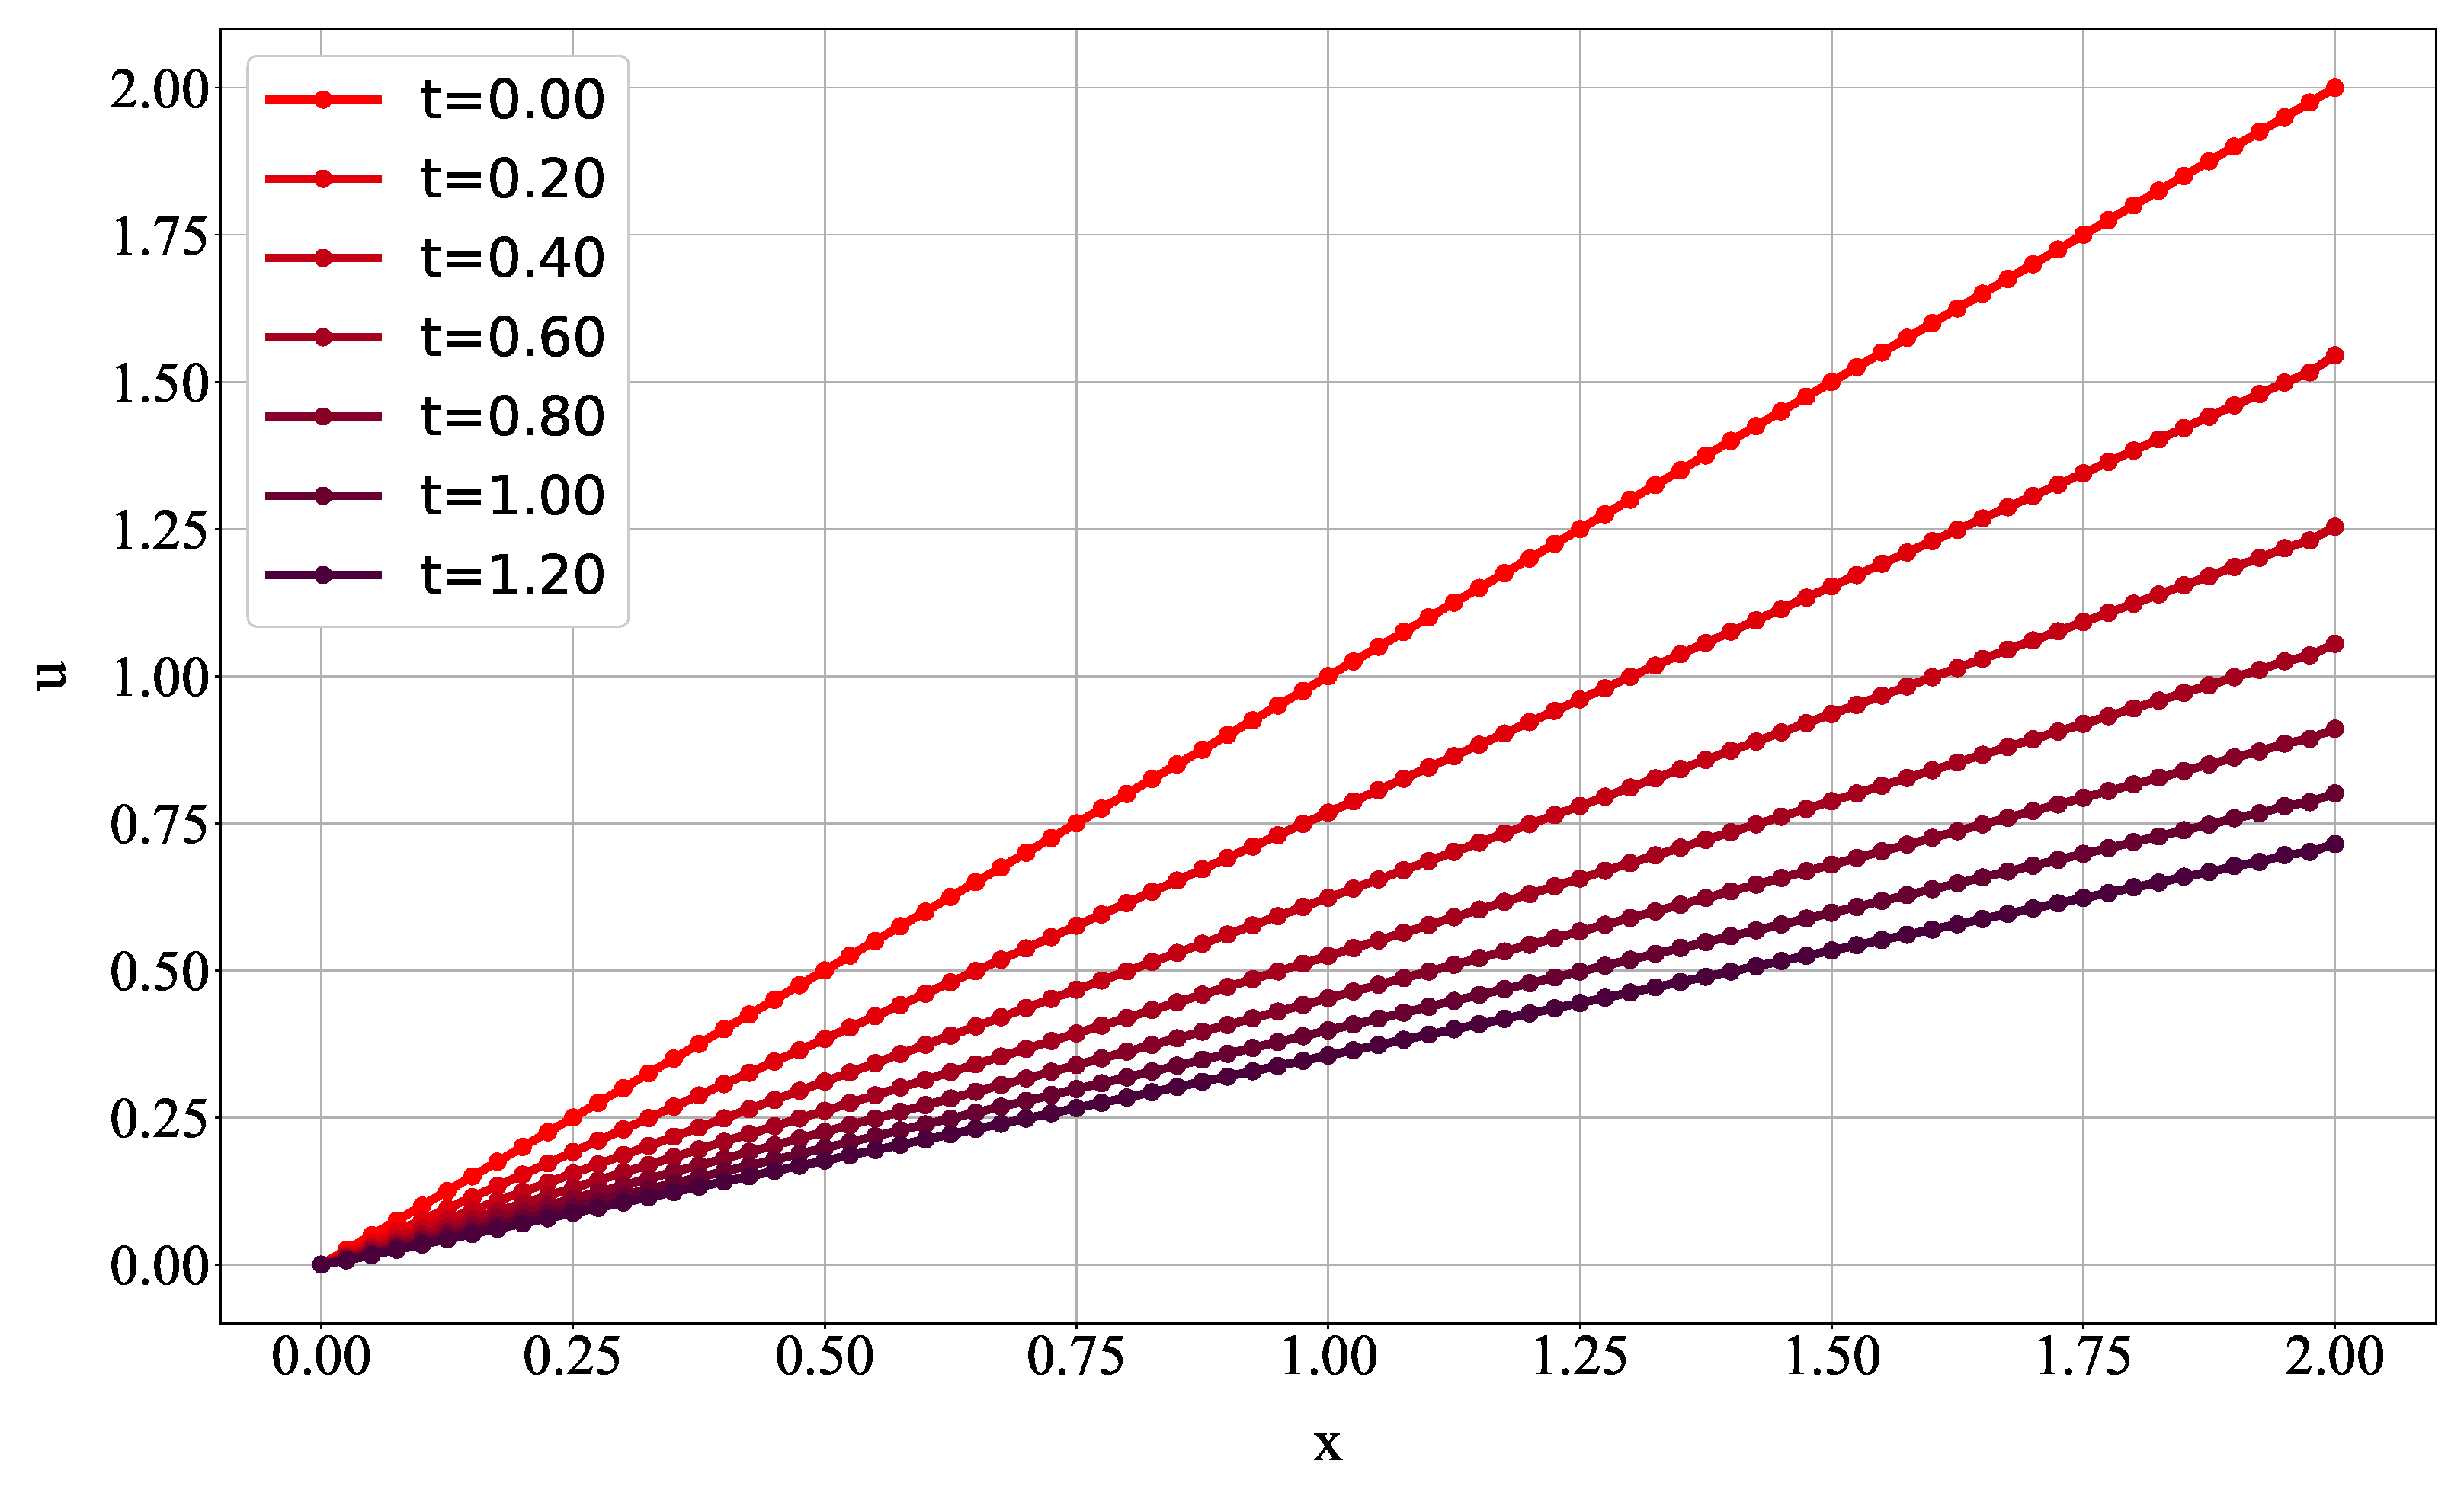
\includegraphics[width=0.425\linewidth]{5.maccormack.cour05.f2025}}\\
      %\cmidrule{3-4}
      {}                                          & $0.9$    &
        \raisebox{-0.5\totalheight}{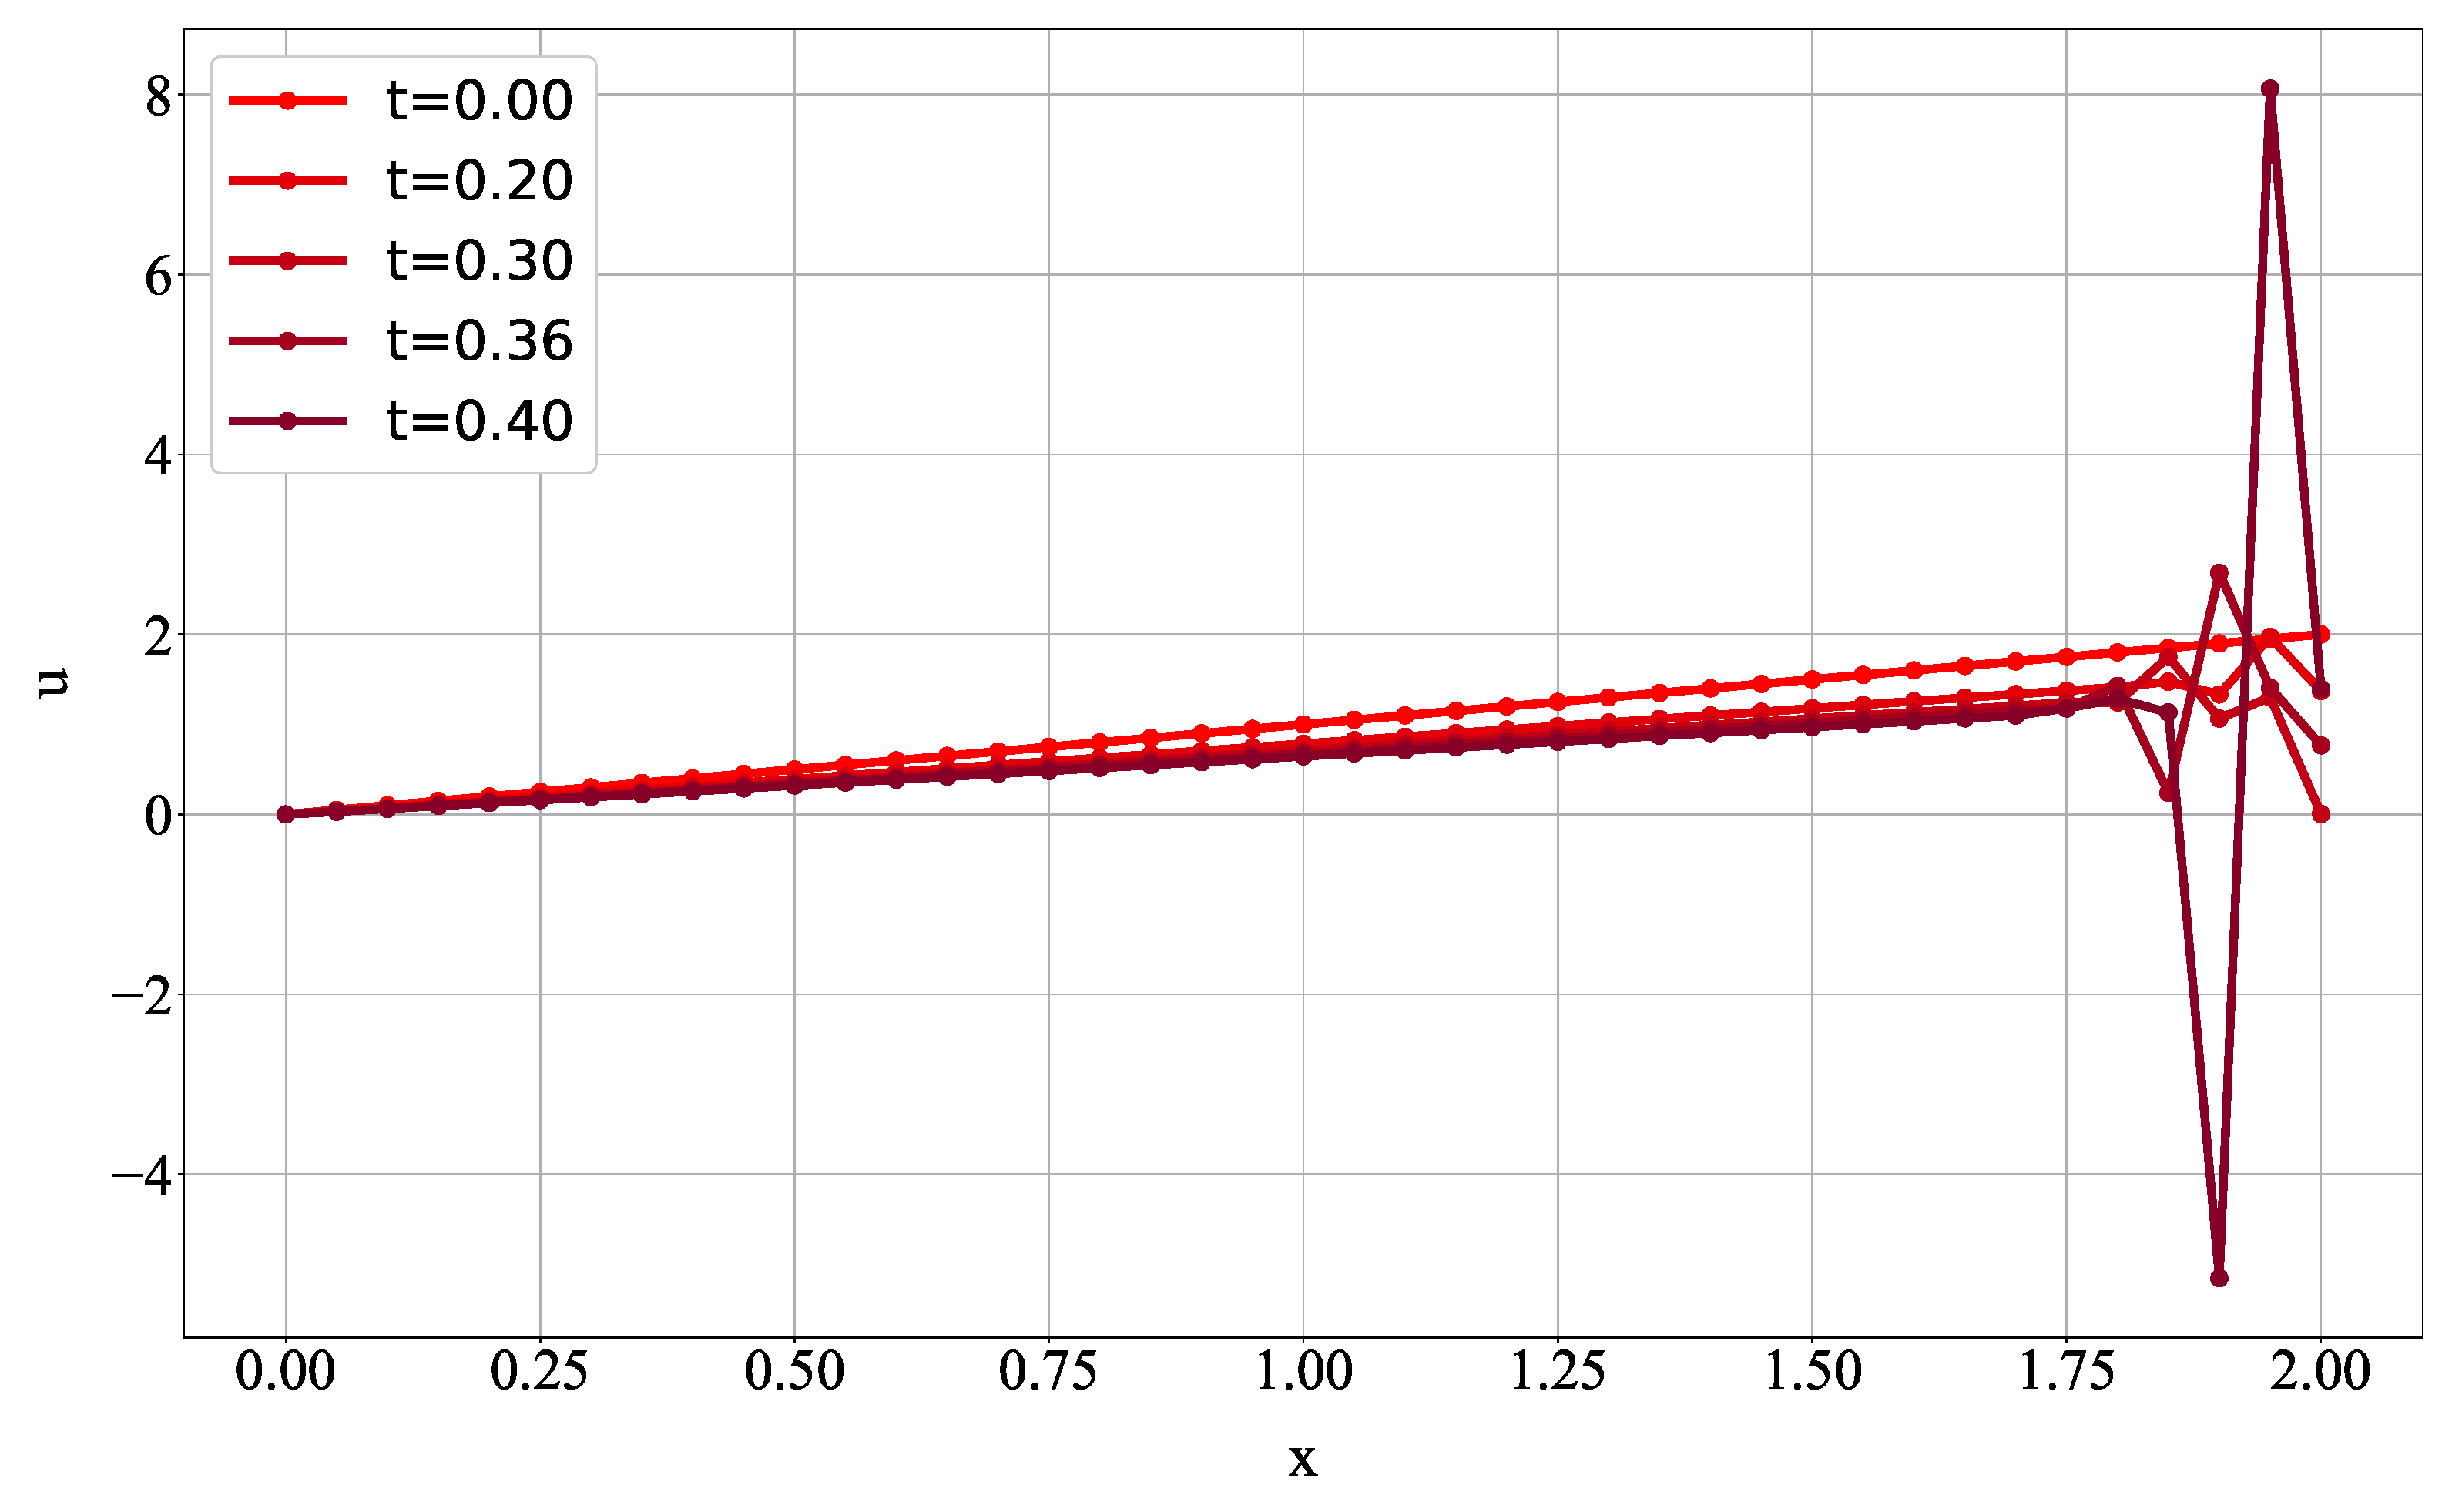
\includegraphics[width=0.425\linewidth]{5.maccormack.cour09.f2050}} &
        \raisebox{-0.5\totalheight}{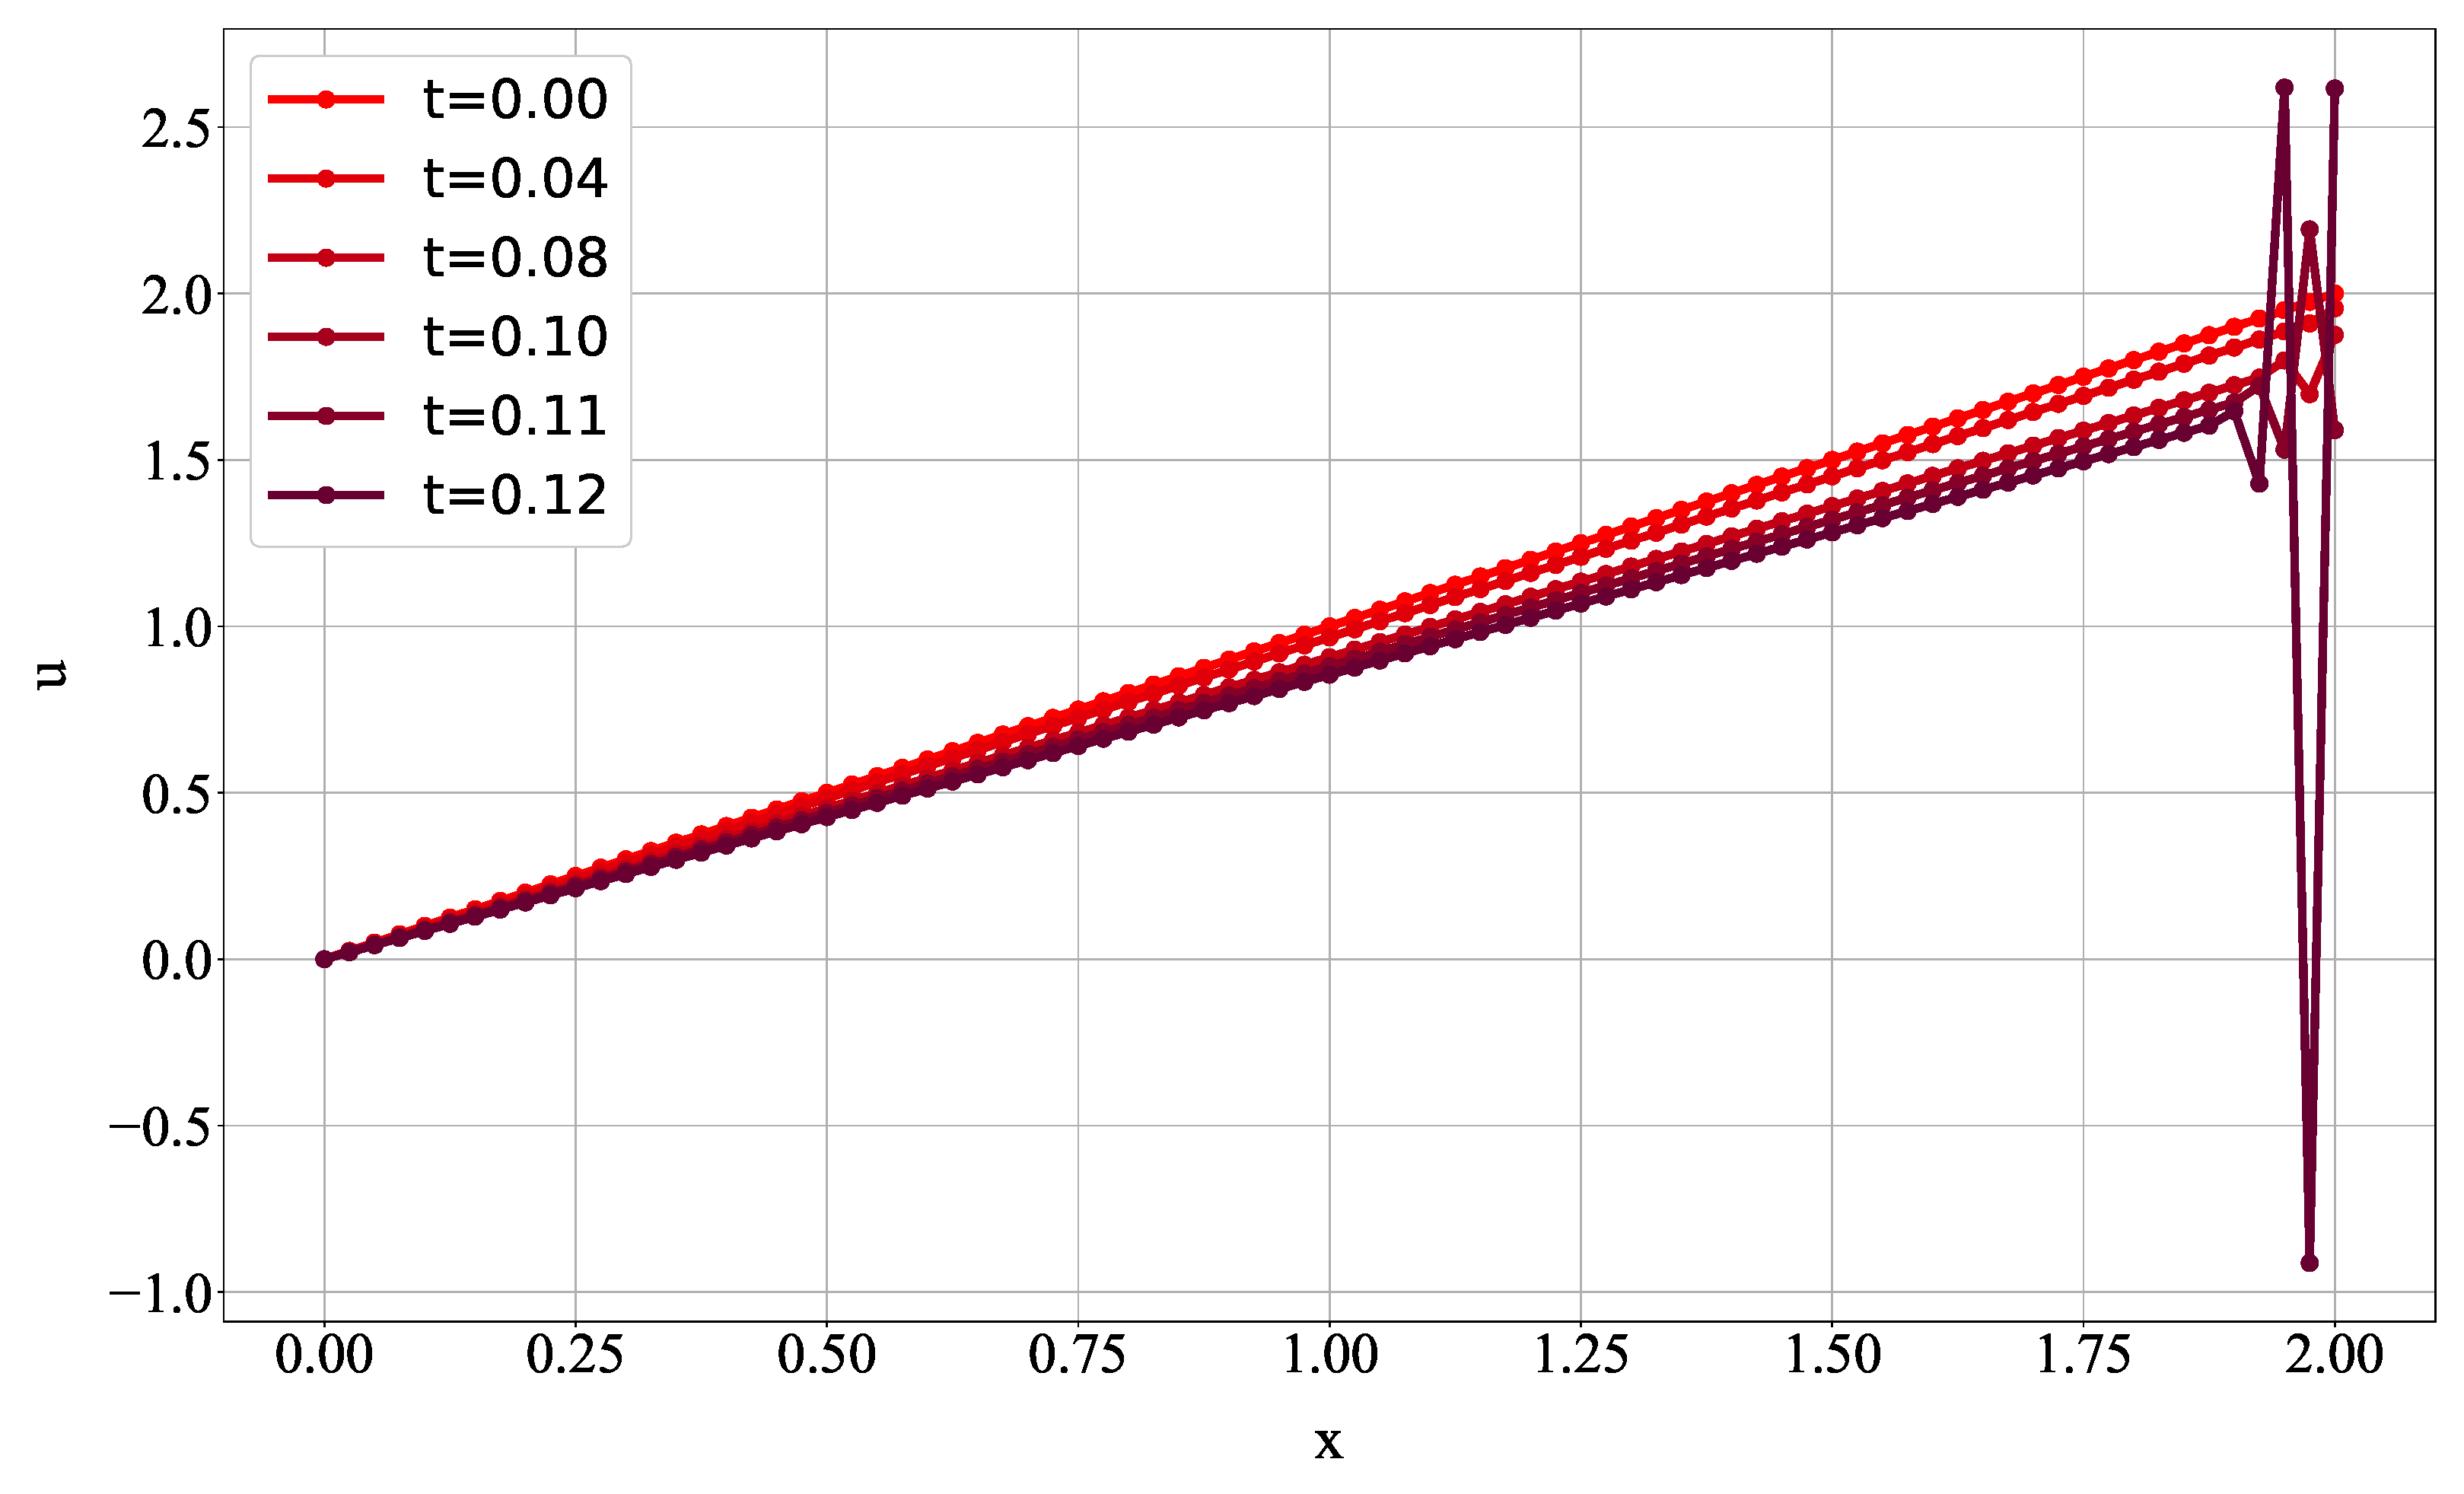
\includegraphics[width=0.425\linewidth]{5.maccormack.cour09.f2025}}\\
      \bottomrule
    \end{tabular}
  \end{center}
  \end{table}
\end{document}